% !TeX root = ../Book5.tex
% 纲要标题：# 第三编　Lie 代数、根系与最高权
% 纲要位置：工作记录/计划纲要.md，第 4081 行。

\BookPart{Lie 代数、根系与最高权}{b5:part:03}
\BookPartGuide
有限群的元素通过可逆矩阵作用，Lie 代数则以线性算子之间的括号为出发点。本编主要讨论有限维复 Lie 代数，最高权分类也限于有限维表示；改变基域、特征或维数范围时，将另行说明条件。

\ProseParagraphBreak
\chapref{b5:ch:11}建立括号、理想、表示及两种下降列。\chapref{b5:ch:12}用 Engel 定理\footnote{恩格尔（Friedrich Engel，1861-1941），德国数学家，与李合作奠定了 Lie 群理论的基础，并研究 Lie 代数的幂零性。}与 Lie 定理解释幂零性、可解性及同时三角化，\chapref{b5:ch:13}再以 Killing 型\footnote{基灵（Wilhelm Killing，1847-1923），德国数学家，开创了复单 Lie 代数的分类研究。}判断半单性，并分解为单理想。一般完全可约性将在\chapref{b5:ch:18}由 Casimir 方法\footnote{卡西米尔（Hendrik Brugt Gerhard Casimir，1909-2000），荷兰物理学家，研究量子理论与凝聚态物理；以其名字命名的不变量也用于 Lie 代数表示论。}证明。Levi 分解\footnote{列维（Eugenio Elia Levi，1883-1917），意大利数学家，证明了有限维 Lie 代数关于可解根的分解定理。}在\secref{b5:sec:1204}给出陈述和交换核的计算，一般存在性与共轭性的证明见\secref{b5:sec:2003}。

\ProseParagraphBreak
\chapref{b5:ch:14}单独研究 \(\mathfrak{sl}_2\)。升降算子确定不可约权链，Casimir 算子帮助证明有限维表示完全可约。\chapref{b5:ch:15}随后用有序单项式和 Jacobi 恒等式证明 PBW，把诱导表示及最高权关系放进泛包络代数中。

\ProseParagraphBreak
\chapref{b5:ch:16}先建立内在 Jordan 分解和 Cartan 子代数，再通过根空间中的 \(\mathfrak{sl}_2\) 三元组证明根弦、整数性和反射。\chapref{b5:ch:17}以这些数据研究 Weyl 群及全部有限约化结晶根系；\secref{b5:sec:1704}再以 Serre 展示\footnote{塞尔（Jean-Pierre Serre，1926-），法国数学家，在代数几何、代数数论与同调方法方面作出重要贡献。}证明相应复半单 Lie 代数的存在与唯一性。这一步完成的是 Lie 代数本身的分类。

\ProseParagraphBreak
\chapref{b5:ch:18}先证明完全可约性，再构造 Verma 模\footnote{维尔马（Daya-Nand Verma，1933-2012），印度数学家，研究半单 Lie 代数的最高权表示，尤其是后来以他命名的诱导模。}，并用支配整权分类\emph{给定}复半单 Lie 代数的有限维简单模。简单模的存在性由简单根方向的幂关系及权集的有限性证明。\chapref{b5:ch:19}随后把 Casimir 的权空间迹整理为 Freudenthal 递推\footnote{弗罗伊登塔尔（Hans Freudenthal，1905-1990），德裔荷兰数学家，研究 Lie 群与表示论，也对数学教育作出贡献。}，结合 Weyl 分母与反对称性，证明特征标公式及维数公式；第7章的 Schur 函数在最后给出 A 型的组合解释，BGG 消解\footnote{BGG 是伯恩斯坦（\OriginalName{Иосиф Наумович Бернштейн}，1945-）、伊斯拉埃尔·盖尔范德（\OriginalName{Израиль Моисеевич Гельфанд}，1913-2009）与谢尔盖·盖尔范德（\OriginalName{Сергей Израилевич Гельфанд}，1944-）三位数学家姓氏的首字母。伯恩斯坦是俄裔以色列数学家，两位盖尔范德是俄罗斯数学家；他们在 Lie 代数表示论中建立了相关消解。}留待后文介绍。

\ProseParagraphBreak
\chapref{b5:ch:10}与本编都出现 Dynkin 图和正根，但参数的对象不同：在 Dynkin 箭图情形，正根给出不可分解表示的维数向量；在这里，支配整权给出固定复半单 Lie 代数的有限维简单模。前一对应由反射函子建立。

\ProseParagraphBreak
计算中应始终看清归一化。本编的一般根内积由 Killing 型诱导，不统一把所有长根的平方长度改成二；分类所用的 Euclid 坐标\footnote{欧几里得（\OriginalName{Εὐκλείδης}，约公元前325-约公元前265），古希腊数学家，著有《几何原本》，系统整理了古典几何。}只作为整体相似的模型。第14—15章的 \(\mathfrak{sl}_2\) 算子 \(h^2+2h+4fe\) 是其 Killing Casimir 的八倍，进入一般公式时会明确换算。主要参考 Humphreys 的《Introduction to Lie Algebras and Representation Theory》\cite[Chapters II--VI]{Humphreys1972LieAlgebras}，所引页码采用1980年修订重印本；该版本的原版权年份为1972年。

% !TeX root = ../../Book5.tex
% 纲要标题：## 第11章　Lie 代数及其表示
% 纲要位置：工作记录/计划纲要.md，第 4083 行。

\chapter{Lie 代数及其表示}
\label{b5:ch:11}
\BookChapterNumber{b5:ch:11}

\begin{chapterabstract}
本章从矩阵交换子引入 Lie 括号，建立子代数、理想、商、导子和伴随表示。随后定义 Lie 代数的模，推导对偶、张量及同态空间上的作用，并以具体表示区分不可约、不可分解与完全可约。最后介绍导出列和下降中心列，明确可解、幂零、半单与单 Lie 代数的含义，说明复数域与正特征中的重要差别。
\end{chapterabstract}

\begin{learninggoals}
\begin{itemize}
\item 能检验交替性和 Jacobi 恒等式，认识矩阵交换子和保持双线性型的经典例子。
\item 区分子代数与理想，正确构造商并计算同态的核、像和交换化。
\item 计算中心、导子和伴随表示，说明伴随作用的核怎样遗失中心信息。
\item 推导对偶作用中的负号和张量作用的加法规则，并判断子空间是否不变。
\item 会计算两种结构列，并用例子辨别可解性、幂零性和半单性。
\end{itemize}
预备知识为有限维线性代数、矩阵乘法、双线性型和张量积，以及前两编的表示、子模和商模观念。这里不要求先学习 Lie 群、流形或 Haar 测度。除明确说明的一般域计算外，本编后续核心结构定理将采用有限维复 Lie 代数。
\end{learninggoals}

有限群表示把群元素送到可逆算子；Lie 代数表示则把 Lie 括号送到算子交换子。两者共享大量线性代数构造，作用公式却并不相同。小矩阵给出逐项核验这些公式的直接例子，同样的计算随后推广到抽象向量空间。Lie 代数和表示的基本定义及例子可参阅\cite[Section 2.9, pp.~22--25]{EtingofEtAl2011RepresentationTheory}；本章始终把交替条件单独写出，以兼顾特征二。

% 纲要范围：
%
% > 本编核心以有限维复 Lie 代数为统一默认对象；改变基域或特征时另行列出假设。无需先学 Lie 群、流形或 Haar 测度。
%

% !TeX root = ../../Book5.tex
% 纲要标题：### 11.1 定义与例子
% 纲要位置：工作记录/计划纲要.md，第 4087 行。

\section{定义与例子}
\label{b5:sec:1101}


% 纲要范围：
%
% * 反对称括号与 Jacobi 恒等式
% * 矩阵交换子及经典 Lie 代数
% * 结合代数到 Lie 代数的构造
%

矩阵乘法一般不交换。若只取两种乘法次序的差，就得到一个双线性运算；它不再满足结合律，却满足另一条控制三重运算的恒等式。Lie 代数把这种括号运算本身作为研究对象。定义不需要 Lie 群或微分流形，本编的主要结构定理则固定在有限维复数情形。

\subsection{反对称括号与 Jacobi 恒等式}
\label{b5:subsec:1101:01}

\begin{definition}\label{b5:def:lie-algebra}
设 \(k\) 为域，\(\mathfrak g\) 为 \(k\) 向量空间。给定 \(k\) 双线性映射
\[
[\ ,\ ]:\mathfrak g\times\mathfrak g\longrightarrow\mathfrak g
\]
使对任意 \(x,y,z\in\mathfrak g\) 都有
\[
[x,x]=0,\qquad
\bigl[x,[y,z]\bigr]+\bigl[y,[z,x]\bigr]+\bigl[z,[x,y]\bigr]=0,
\]
就称 \(\mathfrak g\) 为 \(k\) 上的\term[lie-daishu]{Lie 代数}[Lie algebra]，称第二个恒等式为\term[Jacobi-hengdengshi]{Jacobi 恒等式}[Jacobi identity]。运算 \([x,y]\) 称为 Lie 括号。
\end{definition}
第一条称为交替性。将 \(x+y\) 代入它，得到
\([x,y]=-[y,x]\)，即反对称性。特征不为二时，反对称性反过来推出交替性；特征二时却不能如此，所以一般域上的定义保留 \([x,x]=0\)。
\ProseParagraphBreak
给定一组基 \(x_1,\ldots,x_n\)，括号由
\([x_i,x_j]=\sum_\ell c_{ij}^{\ell}x_\ell\)
决定。这些结构常数必须满足交替条件与 Jacobi 的二次关系。给定基向量之间的括号后，还须检查三重括号的 Jacobi 恒等式。
\begin{example}\label{b5:exm:abelian-heisenberg-lie}
在任意向量空间上令全部括号为零，就得到交换 Lie 代数。另取基 \(x,y,z\)，规定 \([x,y]=z\)、\([x,z]=[y,z]=0\)，并按交替双线性延拓。每个括号都在 \(kz\)，而 \(z\) 与全部元素括号为零，所以所有三重括号均为零，Jacobi 恒等式成立。这是三维\term[Heisenberg-lie-daishu]{Heisenberg Lie 代数}[Heisenberg Lie algebra]。
\end{example}
Jacobi 恒等式也可写成
\[
\bigl[x,[y,z]\bigr]=\bigl[[x,y],z\bigr]+\bigl[y,[x,z]\bigr].
\]
它说明固定 \(x\) 后，“与 \(x\) 取括号”像求导一样作用于另一个括号。这个形式将在理想、导子和表示中反复出现。

\subsection{矩阵交换子及经典 Lie 代数}
\label{b5:subsec:1101:02}

\begin{proposition}\label{b5:prop:commutator-lie-algebra}
设 \(A\) 为域 \(k\) 上的结合代数，不要求交换。规定
\[
[x,y]=xy-yx.
\]
则 \(A\) 的底层向量空间成为 Lie 代数，记为 \(A^{-}\)。
\end{proposition}
\begin{proof}
双线性和 \([x,x]=0\) 直接成立。结合律使三项展开为
\[
\begin{aligned}
\bigl[x,[y,z]\bigr]&=xyz-xzy-yzx+zyx,\\
\bigl[y,[z,x]\bigr]&=yzx-yxz-zxy+xzy,\\
\bigl[z,[x,y]\bigr]&=zxy-zyx-xyz+yxz.
\end{aligned}
\]
相加后每个三重乘积出现两次，符号相反，所以和为零。这个证明不使用特征限制。
\end{proof}
特别地，\(\operatorname{End}_k(V)^{-}\) 记为
\(\mathfrak{gl}(V)\)；选基后写为 \(\mathfrak{gl}_n(k)\)。
满足 \(\operatorname{tr}X=0\) 的矩阵组成子空间 \(\mathfrak{sl}_n(k)\)，它对括号封闭，因为
\(\operatorname{tr}(XY)=\sum_{i,j}x_{ij}y_{ji}=\operatorname{tr}(YX)\)。
\symidx{\(\mathfrak{gl}(V),\mathfrak{sl}_n(k)\)：一般线性与特殊线性 Lie 代数}
\ProseParagraphBreak
对可逆对称矩阵 \(B\) 和标准交替矩阵
\(J=\begin{psmallmatrix}0&I_n\\-I_n&0\end{psmallmatrix}\)，还可定义
\[
\begin{aligned}
\mathfrak{so}(B)&=\{\,X\mid X^{\mathsf T}B+BX=0\,\},\\
\mathfrak{sp}_{2n}(k)&=\{\,X\mid X^{\mathsf T}J+JX=0\,\}.
\end{aligned}
\]
第一式讨论正交情形时，本编假设 \(\operatorname{char}k\ne2\)。这些条件的含义是：矩阵 \(X\) 满足
\(b(Xu,v)+b(u,Xv)=0\)，其中 \(b\) 为相应双线性型。
若 \(X,Y\) 都满足这个条件，两次使用它得到
\[
b(XYu,v)=b(u,YXv),\qquad b(YXu,v)=b(u,XYv),
\]
相减便证明 \([X,Y]\) 仍满足条件。因此这两个子空间都是 Lie 代数。
\symidx{\(\mathfrak{so}(B),\mathfrak{sp}_{2n}(k)\)：正交与辛 Lie 代数}
本编还会研究上三角矩阵 Lie 代数 \(\mathfrak b_n\) 与严格上三角矩阵 Lie 代数 \(\mathfrak n_n\)。它们都是矩阵乘法下的子代数，因而也对交换子封闭。矩阵群中要求可逆，矩阵 Lie 代数中则没有这个要求；零矩阵就在所有这些 Lie 代数中。

\subsection{结合代数到 Lie 代数的构造}
\label{b5:subsec:1101:03}

从 \(A\) 到 \(A^{-}\) 会忘掉部分结合乘法信息。例如一个交换代数的全部 Lie 括号都是零，单靠这个零括号不能恢复原来的多项式乘法或幂零元。
\begin{proposition}\label{b5:prop:associative-map-lie-map}
设 \(k\) 为域，\(A,B\) 为 \(k\) 上的结合代数，\(f:A\to B\) 为 \(k\) 代数同态。对任意 \(x,y\in A\)，其底层线性映射保持交换子：
\[
f\bigl([x,y]\bigr)=\bigl[f(x),f(y)\bigr].
\]
如果 \(A\) 有单位，给定一个幺性左 \(A\) 模便得到交换子 Lie 代数 \(A^{-}\) 的线性作用；但任意保持 Lie 括号的映射未必保持结合乘法或单位。
\end{proposition}
\begin{proof}
计算 \(f(xy-yx)=f(x)f(y)-f(y)f(x)\)。对模的作用同态 \(A\to\operatorname{End}_k(V)\) 应用此等式，就得到括号相容性。反向断言的失败已经可在交换代数中看见：例如 \(\mathbb C\to\mathbb C\)、\(z\mapsto2z\)，保持两个零括号，却不保持单位或乘法。
\end{proof}
因此“结合代数的表示”和“相应 Lie 代数的表示”不是同一类数据。\chapref{b5:ch:15}将构造泛包络代数，使一个给定 Lie 代数的全部表示恰好等同于某个结合代数的模；那是对 Lie 括号另作构造，不能简单使用本节原来的 \(A\)。

% !TeX root = ../../Book5.tex
% 纲要标题：### 11.2 子代数、理想与商
% 纲要位置：工作记录/计划纲要.md，第 4093 行。

\section{子代数、理想与商}
\label{b5:sec:1102}


% 纲要范围：
%
% * 同态及同构定理
% * 中心与导子
% * 伴随表示
%

Lie 代数的子对象和商仍须与括号相容。理想条件保证一个括号在取商后不依赖代表；伴随表示则把这种相容性写成线性算子的交换关系。这些构造是后面分解 Lie 代数的基础。

\subsection{同态及同构定理}
\label{b5:subsec:1102:01}

\begin{definition}\label{b5:def:lie-subalgebra-ideal}
设 \(\mathfrak g\) 为域 \(k\) 上的 Lie 代数。子空间 \(\mathfrak h\subseteq\mathfrak g\) 若满足 \([\mathfrak h,\mathfrak h]\subseteq\mathfrak h\)，就称为子代数；子空间 \(\mathfrak a\subseteq\mathfrak g\) 若满足 \([\mathfrak g,\mathfrak a]\subseteq\mathfrak a\)，就称为理想。这里 \([U,W]\) 表示所有 \([u,w]\)、\(u\in U,w\in W\) 的线性生成空间。
\end{definition}
\begin{definition}\label{b5:def:lie-homomorphism}
设 \(\mathfrak g,\mathfrak l\) 为同一域 \(k\) 上的 Lie 代数。一个 \(k\) 线性映射 \(f:\mathfrak g\to\mathfrak l\) 若满足
\(f\bigl([x,y]\bigr)=\bigl[f(x),f(y)\bigr]\) 对所有 \(x,y\in\mathfrak g\) 成立，就称为 Lie 代数同态；若它还是线性同构，就称为 Lie 代数同构。
\end{definition}
例如上三角矩阵在 \(\mathfrak{gl}_n(k)\) 中为子代数，严格上三角矩阵在上三角代数中为理想。后一空间通常不是整个 \(\mathfrak{gl}_n(k)\) 的理想：在二维中，
\([E_{21},E_{12}]=E_{22}-E_{11}\)
不再严格上三角。理想的环境不能从叙述中省去。
\begin{proposition}\label{b5:prop:lie-isomorphism}
设 \(\mathfrak g,\mathfrak l\) 为同一域 \(k\) 上的 Lie 代数，\(f:\mathfrak g\to\mathfrak l\) 为 Lie 代数同态。则 \(\ker f\) 为 \(\mathfrak g\) 的理想，\(\operatorname{im}f\) 为 \(\mathfrak l\) 的子代数，且
\[
\mathfrak g/\ker f\cong\operatorname{im}f.
\]
更一般地，对 \(\mathfrak g\) 的理想 \(\mathfrak a\)，商空间上的括号
\([x+\mathfrak a,y+\mathfrak a]=[x,y]+\mathfrak a\)
良定义；包含 \(\mathfrak a\) 的理想与商 Lie 代数的理想一一对应。
\end{proposition}
\begin{proof}
若 \(x\in\ker f\)，则 \(f\bigl([y,x]\bigr)=\bigl[f(y),0\bigr]=0\)，证明核为理想；像对括号封闭直接由同态等式得到。若更换两个商代表，括号的差为
\([a,y]+[x,b]+[a,b]\)，其中 \(a,b\in\mathfrak a\)，各项都在理想中，故良定义。双线性、交替性与 Jacobi 从原代数下降。映射 \(x+\ker f\mapsto f(x)\) 线性双射并保持括号，得到同构。最后，理想沿商映射取像或逆像时分别保持括号相容条件，两种操作互逆。
\end{proof}
同样的计算还给出第二、第三同构定理。例如若 \(\mathfrak h\) 为子代数、\(\mathfrak a\) 为理想，则
\(\mathfrak h/(\mathfrak h\cap\mathfrak a)\cong(\mathfrak h+\mathfrak a)/\mathfrak a\)；
若 \(\mathfrak a\subseteq\mathfrak b\) 为理想，则
\((\mathfrak g/\mathfrak a)/(\mathfrak b/\mathfrak a)\cong\mathfrak g/\mathfrak b\)。
这些映射分别由包含和复合商映射给出，核与像已由前一命题确定。

\subsection{中心与导子}
\label{b5:subsec:1102:02}

\begin{definition}\label{b5:def:lie-center-derivations}
设 \(\mathfrak g\) 为域 \(k\) 上的 Lie 代数。其中心为
\[
Z(\mathfrak g)=\bigl\{\,z\in\mathfrak g\mid[z,x]=0\;\text{对所有}\;x\in\mathfrak g\,\bigr\}.
\]
\(k\) 线性映射 \(D:\mathfrak g\to\mathfrak g\) 若对所有 \(x,y\in\mathfrak g\) 满足
\[
D\bigl([x,y]\bigr)=\bigl[D(x),y\bigr]+\bigl[x,D(y)\bigr],
\]
就称为 \(\mathfrak g\) 的\term[lie-daishu-daozi]{导子}[derivation of a Lie algebra]。全部导子的空间记为 \(\operatorname{Der}(\mathfrak g)\)。
\end{definition}
\symidx{\(Z(\mathfrak g),\operatorname{Der}(\mathfrak g)\)：Lie 代数的中心与导子代数}
中心是一个交换理想。对一个子空间 \(U\subseteq\mathfrak g\)，还分别定义
\[
C_{\mathfrak g}(U)=\bigl\{\,x\mid[x,U]=0\,\bigr\},\qquad
N_{\mathfrak g}(U)=\bigl\{\,x\mid[x,U]\subseteq U\,\bigr\},
\]
称为中心化子与正规化子。若 \(U\) 是子代数，Jacobi 恒等式说明这两者也是子代数。
\symidx{\(C_{\mathfrak g}(U),N_{\mathfrak g}(U)\)：Lie 代数中子空间的中心化子与正规化子}
\begin{proposition}\label{b5:prop:lie-derivations}
设 \(\mathfrak g\) 为域 \(k\) 上的 Lie 代数。导子空间 \(\operatorname{Der}(\mathfrak g)\) 在算子交换子下组成 Lie 代数。对每个 \(x\in\mathfrak g\)，映射
\[
\operatorname{ad}x:\mathfrak g\longrightarrow\mathfrak g,\qquad
y\longmapsto[x,y]
\]
为导子，并对每个 \(D\in\operatorname{Der}(\mathfrak g)\) 满足
\[
[D,\operatorname{ad}x]=\operatorname{ad}(D x).
\]
因此这些内导子的空间 \(\operatorname{ad}\mathfrak g\) 为 \(\operatorname{Der}(\mathfrak g)\) 的理想。
\end{proposition}
\symidx{\(\operatorname{ad}x\)：Lie 代数元素的伴随作用}
\begin{proof}
对导子 \(D,E\)，将 \(DE\bigl([x,y]\bigr)-ED\bigl([x,y]\bigr)\) 展开，混合项
\(\bigl[D(x),E(y)\bigr]\)、\(\bigl[E(x),D(y)\bigr]\) 成对消去，剩下
\(\bigl[[D,E]x,y\bigr]+\bigl[x,[D,E]y\bigr]\)，所以交换子仍为导子。Jacobi 的导子形式直接说明 \(\operatorname{ad}x\) 为导子。再对 \(y\) 计算
\(D\bigl([x,y]\bigr)-\bigl[x,D(y)\bigr]=[Dx,y]\)，得到最后的等式。
\end{proof}
导子未必都为内导子。例如一维交换 Lie 代数的全部内导子为零，每个线性自同态却都是导子。半单复 Lie 代数中的情况将不同，但不能把那个结论用于当前任意 Lie 代数。

\subsection{伴随表示}
\label{b5:subsec:1102:03}

\begin{proposition}\label{b5:prop:adjoint-representation}
设 \(\mathfrak g\) 为域 \(k\) 上的 Lie 代数。映射
\[
\operatorname{ad}:\mathfrak g\longrightarrow\mathfrak{gl}(\mathfrak g),
\qquad x\longmapsto\operatorname{ad}x
\]
是 Lie 代数同态，其核为 \(Z(\mathfrak g)\)。一个子空间 \(\mathfrak a\subseteq\mathfrak g\) 在所有 \(\operatorname{ad}x\) 下不变，当且仅当它是理想。
\end{proposition}
\begin{proof}
对 \(z\in\mathfrak g\)，Jacobi 恒等式给出
\[
[\operatorname{ad}x,\operatorname{ad}y](z)
=\bigl[x,[y,z]\bigr]-\bigl[y,[x,z]\bigr]
=\bigl[[x,y],z\bigr].
\]
故它保持括号。核与不变子空间两项结论分别就是中心和理想的定义。
\end{proof}
这称为\term[bansui-biaoshi]{伴随表示}[adjoint representation]。它把 Lie 代数的内部括号转成一组线性算子，因而可用特征值、迹与三角化研究结构。但它一般不忠实：三维 Heisenberg 代数中的 \(z\) 就全部作用为零，伴随表示看见的是模去中心后的代数。
\ProseParagraphBreak
例如二维代数取基 \(h,e\)，规定 \([h,e]=e\)。在这组基下，
\[
\operatorname{ad}h=\begin{pmatrix}0&0\\0&1\end{pmatrix},
\qquad
\operatorname{ad}e=\begin{pmatrix}0&0\\-1&0\end{pmatrix}.
\]
两矩阵的交换子等于第二个矩阵，与原来的关系一致。这个小例子以后将区分可解性与幂零性。

% !TeX root = ../../Book5.tex
% 纲要标题：### 11.3 表示与模
% 纲要位置：工作记录/计划纲要.md，第 4099 行。

\section{表示与模}
\label{b5:sec:1103}


% 纲要范围：
%
% * Lie 代数的线性作用
% * 对偶和张量表示
% * 不变子空间及完全可约性的提问
%

Lie 代数的表示仍然由线性算子组成，但相容条件针对的是括号。一个元素无需作用为可逆算子，也没有“先求群元素的逆”的步骤。对偶与张量作用中的符号应从这个条件重新推导，不能照搬群表示的公式。

\subsection{Lie 代数的线性作用}
\label{b5:subsec:1103:01}

\begin{definition}\label{b5:def:lie-representation}
设 \(\mathfrak g\) 为域 \(k\) 上的 Lie 代数，\(V\) 为 \(k\) 向量空间。一个 \(k\) 线性映射
\(\rho:\mathfrak g\to\mathfrak{gl}(V)\)
若满足
\[
\rho\bigl([x,y]\bigr)=\rho(x)\rho(y)-\rho(y)\rho(x)
\quad(x,y\in\mathfrak g),
\]
就称为 \(\mathfrak g\) 在 \(V\) 上的\term[lie-daishu-biaoshi]{表示}[representation of a Lie algebra]，也称 \(V\) 为左 \(\mathfrak g\) 模。简记 \(xv=\rho(x)v\)；此时相容条件为
\[
[x,y]v=x(yv)-y(xv).
\]
\end{definition}
设 \(\rho_V,\rho_W\) 分别为 \(\mathfrak g\) 在 \(V,W\) 上的表示。线性映射 \(T:V\to W\) 若满足
\[
T\rho_V(x)=\rho_W(x)T\quad(x\in\mathfrak g),
\]
即 \(T(xv)=xT(v)\)，就称为表示同态；两个表示同构要求这样的同态可逆。当 \(V=W\) 且两表示相同时，这一条件才表示 \(T\) 与全部作用算子对易。子表示是被全部作用算子保持的子空间，商表示由商空间上的诱导算子给出。若 \(\rho\) 单射，称表示忠实；若全部作用为零，称表示平凡。
\ProseParagraphBreak
\cref{b5:prop:adjoint-representation}给出了伴随表示。矩阵 Lie 代数作为 \(\mathfrak{gl}_n(k)\) 的子代数时，还在 \(k^n\) 上有自然表示。另一个简单例子是一维模：它由线性泛函 \(\lambda:\mathfrak g\to k\) 决定，作用为 \(xv=\lambda(x)v\)。表示条件恰好要求
\(\lambda\bigl([\mathfrak g,\mathfrak g]\bigr)=0\)，因为一维算子彼此交换。故一维模与交换化商 \(\mathfrak g/[\mathfrak g,\mathfrak g]\) 上的线性泛函对应。
\begin{proposition}\label{b5:prop:lie-invariant-subquotients}
设 \(\mathfrak g\) 为域 \(k\) 上的 Lie 代数，\(V,W\) 为左 \(\mathfrak g\) 模，\(f:V\to W\) 为表示同态。则核、像与余核均自然为左 \(\mathfrak g\) 模；一列左 \(\mathfrak g\) 模正合，当且仅当底层 \(k\) 向量空间列正合。
\end{proposition}
\begin{proof}
若 \(f(v)=0\)，则 \(f(xv)=xf(v)=0\)，故核不变。若 \(w=f(v)\)，则 \(xw=f(xv)\) 仍在像中。于是商上的作用不依赖代表，且表示等式从原空间下降。核、像和商都没有改变相应的向量空间运算，所以正合性也按底层空间检验。
\end{proof}

\subsection{对偶表示与张量表示}
\label{b5:subsec:1103:02}

若要求求值 \(V^*\otimes V\to k\)、\(\varphi\otimes v\mapsto\varphi(v)\) 是表示同态，而 \(k\) 上的作用平凡，那么必有
\[
0=x\cdot\varphi(v)=(x\varphi)(v)+\varphi(xv).
\]
这便迫使对偶作用带负号。张量作用的两项之和则可从一次项看出：在 \(\varepsilon^2=0\) 时，
\[
(I+\varepsilon\rho_V(x))v\otimes(I+\varepsilon\rho_W(x))w
=v\otimes w+\varepsilon(xv\otimes w+v\otimes xw).
\]
下面还须核验这些由相容性要求得到的公式确实满足 Lie 括号关系。

\begin{proposition}\label{b5:prop:lie-dual-tensor-hom}
设 \(\mathfrak g\) 为域 \(k\) 上的 Lie 代数，\(\rho_V,\rho_W\) 分别为它在 \(k\) 向量空间 \(V,W\) 上的表示。对 \(x\in\mathfrak g\)、\(v\in V\)、\(w\in W\)、\(\varphi\in V^*=\operatorname{Hom}_k(V,k)\) 及 \(T\in\operatorname{Hom}_k(V,W)\)，下列公式分别给出 \(V^*\)、\(V\otimes_k W\) 与 \(\operatorname{Hom}_k(V,W)\) 上的表示；其中 \(xv=\rho_V(x)v\)、\(xw=\rho_W(x)w\)：
\[
\begin{aligned}
(x\varphi)(v)&=-\varphi(xv),\\
x(v\otimes w)&=xv\otimes w+v\otimes xw,\\
xT&=\rho_W(x)T-T\rho_V(x).
\end{aligned}
\]
若 \(V\) 有限维，则自然同构 \(V^*\otimes W\cong\operatorname{Hom}_k(V,W)\) 与这些作用相容。
\end{proposition}
\begin{proof}
在对偶上，先后作用 \(x,y\) 给出
\[
\begin{aligned}
\bigl(x\cdot(y\cdot\varphi)\bigr)(v)&=\varphi\bigl(y(xv)\bigr),\\
\bigl(y\cdot(x\cdot\varphi)\bigr)(v)&=\varphi\bigl(x(yv)\bigr).
\end{aligned}
\]
由 \(V\) 上的表示关系，
\[
\begin{aligned}
\bigl(x\cdot(y\cdot\varphi)-y\cdot(x\cdot\varphi)\bigr)(v)
&=-\varphi\bigl([x,y]v\bigr)\\
&=\bigl([x,y]\cdot\varphi\bigr)(v),
\end{aligned}
\]
正好是对偶上的表示关系。在张量积上，算子为
\(\rho_V(x)\otimes I+I\otimes\rho_W(x)\)；
两个不同因子上的算子交换，计算交换子只留下两个因子的表示关系。对 Hom 展开两次作用，混合项相消，同样得到
\(\rho_W\bigl([x,y]\bigr)T-T\rho_V\bigl([x,y]\bigr)\)。
最后把 \(\varphi\otimes w\) 送到 \(v\mapsto\varphi(v)w\)，代入公式得到
\[
x\bigl(\varphi(v)w\bigr)-\varphi(xv)w
=\varphi(v)xw-\varphi(xv)w,
\]
这正是对偶与张量作用的像。有限维线性代数给出该映射为同构。
\end{proof}
尤其
\[
\operatorname{Hom}_{\mathfrak g}(V,W)
=\operatorname{Hom}_k(V,W)^{\mathfrak g},
\qquad
U^{\mathfrak g}=\{\,u\in U\mid xu=0\text{ 对所有 }x\in\mathfrak g\,\}.
\]
这里“不变”表示被所有 Lie 代数作用零化，与群表示中被所有群元素固定的说法不同。
\ProseParagraphBreak
在 \(V^{\otimes m}\) 上，\(x\) 的作用是分别在各因子作用后相加，并令 \(x1=0\)。将两个张量字拼接时，这些因子分为两组，因而在张量代数 \(T(V)\) 上有
\[
x(u\otimes w)=(xu)\otimes w+u\otimes(xw)
\quad(u,w\in T(V)).
\]
因此每个 \(x\) 在 \(T(V)\) 上作用为导子。对称代数的关系是由 \(v\otimes w-w\otimes v\) 生成的双边理想，而
\[
\begin{aligned}
x(v\otimes w-w\otimes v)
&=(xv\otimes w-w\otimes xv)\\
&\quad +(v\otimes xw-xw\otimes v)
\end{aligned}
\]
仍属于该理想。由导子性质，这个双边理想被作用保持。

外代数的关系理想由平方张量生成。对 \(v\otimes v\) 的作用为
\[
\begin{aligned}
x(v\otimes v)&=xv\otimes v+v\otimes xv\\
&=(xv+v)\otimes(xv+v)-xv\otimes xv-v\otimes v,
\end{aligned}
\]
所以该理想也被保持。因此对称幂、外幂及整个对称代数和外代数都得到诱导作用。在多项式代数上，这个作用满足 Leibniz 规则\footnote{莱布尼茨（Gottfried Wilhelm Leibniz，1646-1716），德国数学家、哲学家，独立创立微积分，并发展了微分记号和乘积求导法则。}，是导子，而不是代数自同构。

\subsection{不变子空间与完全可约性}
\label{b5:subsec:1103:03}

\begin{definition}\label{b5:def:lie-simple-semisimple-module}
设 \(\mathfrak g\) 为域 \(k\) 上的 Lie 代数，\(V\) 为左 \(\mathfrak g\) 模。若 \(V\ne0\) 且没有非零真子表示，就称 \(V\) 为不可约表示；若 \(V\) 是不可约子表示的直和，就称为完全可约表示。若 \(V\ne0\) 且不能分成两个非零子表示的直和，则称为不可分解表示。有限维不可约表示必不可分解，逆命题一般不成立。
\end{definition}
例如二维可解 Lie 代数 \([h,e]=e\) 可在 \(k^2\) 上作用为
\[
\rho(h)=\begin{pmatrix}1&0\\0&0\end{pmatrix},\qquad
\rho(e)=\begin{pmatrix}0&1\\0&0\end{pmatrix}.
\]
两矩阵的交换子等于 \(\rho(e)\)，所以确为表示。第一坐标轴不变，但任何补直线均含第二坐标非零的向量，而 \(\rho(e)\) 将它送到非零第一坐标向量，因而没有不变补。这个表示可约却不可分解。
\ProseParagraphBreak
Schur 引理对 Lie 代数表示仍成立：同态的核与像是子表示，所以不可约之间的非零同态可逆。若基域代数闭且表示有限维，自同态取一个特征值后减去相应标量，就由同一论证得到它原本就是标量。但要从自同态只有标量反推不可约，仍须有额外条件；上一例的两个作用矩阵的公共中心化子就只有标量，却不完全可约。
\ProseParagraphBreak
Lie 代数表示的分解取决于 Lie 代数本身的结构。本编将证明：半单复 Lie 代数的有限维表示完全可约，可解复 Lie 代数的有限维不可约表示只能一维。前一结论需要 Killing 型与 Casimir 方法，后一结论来自同时三角化；两者的假设与证明均不同。

% !TeX root = ../../Book5.tex
% 纲要标题：### 11.4 结构问题
% 纲要位置：工作记录/计划纲要.md，第 4105 行。

\section{结构问题}
\label{b5:sec:1104}


% 纲要范围：
%
% * 可解、幂零及半单的定义
% * 导出代数与导出列
% * 复 Lie 代数与一般正特征 Lie 代数的区别
%
% ---
%

最初的结构问题，是反复取括号以后会发生什么。导出列让两边同时来自上一步，下降中心列则始终允许一边来自整个代数。二者给出的有限终止条件不同；弄清这种区别，才能准确使用下一章的三角化定理。

\subsection{可解、幂零与半单 Lie 代数}
\label{b5:subsec:1104:01}

\begin{definition}\label{b5:def:lie-solvable-nilpotent}
设 \(\mathfrak g\) 为域 \(k\) 上 Lie 代数。定义导出列
\[
\mathfrak g^{(0)}=\mathfrak g,\qquad
\mathfrak g^{(r+1)}=\bigl[\mathfrak g^{(r)},\mathfrak g^{(r)}\bigr],
\]
以及下降中心列
\[
\gamma_1(\mathfrak g)=\mathfrak g,\qquad
\gamma_{r+1}(\mathfrak g)=\bigl[\mathfrak g,\gamma_r(\mathfrak g)\bigr].
\]
若存在整数 \(r\ge0\) 使 \(\mathfrak g^{(r)}=0\)，称 \(\mathfrak g\) \term[kejie-lie-daishu]{可解}[solvable]。此时记
\[
\ell(\mathfrak g)=\min\{r\ge0:\mathfrak g^{(r)}=0\},
\]
称它为 \(\mathfrak g\) 的\term[kejie-changdu]{可解长度}[derived length]。若存在整数 \(c\ge0\) 使 \(\gamma_{c+1}(\mathfrak g)=0\)，称 \(\mathfrak g\) \term[miling-lie-daishu]{幂零}[nilpotent]。此时最小的这种 \(c\) 记为 \(c(\mathfrak g)\)，称为 \(\mathfrak g\) 的幂零类。零 Lie 代数的可解长度与幂零类均为 \(0\)。
\end{definition}
\symidx{\(\mathfrak g^{(r)},\gamma_r(\mathfrak g)\)：Lie 代数的导出列与下降中心列}
\symidx{\(\ell(\mathfrak g),c(\mathfrak g)\)：Lie 代数的可解长度与幂零类}
\begin{definition}\label{b5:def:lie-semisimple-simple}
设 \(\mathfrak g\) 为域 \(k\) 上有限维 Lie 代数。若它没有非零可解理想，就称为\term[bandan-lie-daishu]{半单 Lie 代数}[semisimple Lie algebra]。若它非交换且只有零与自身两个理想，就称为\term[dan-lie-daishu]{单 Lie 代数}[simple Lie algebra]。
\end{definition}
这里把非交换性写入“单”的定义，因而一维交换 Lie 代数不称为单 Lie 代数。半单代数最终能否分解为单理想之和，还需要证明；在定义中先使用理想条件，避免把后面的分解定理预先假定下来。
\ProseParagraphBreak
三维 Heisenberg 代数满足
\(\gamma_2=kz,\gamma_3=0\)，所以幂零类为二。二维代数 \([h,e]=e\) 则满足
\[
\mathfrak g^{(1)}=ke,\quad \mathfrak g^{(2)}=0,\qquad
\gamma_r(\mathfrak g)=ke\quad(r\ge2).
\]
它可解但不幂零。这里的一维理想 \(ke\) 和一维商 \(\mathfrak g/ke\) 都是交换 Lie 代数，已经说明幂零性不能像可解性一样在任意扩张下保持。

\subsection{导出代数与导出列}
\label{b5:subsec:1104:02}

\begin{proposition}\label{b5:prop:lie-derived-ideal}
设 \(\mathfrak g\) 为域 \(k\) 上的 Lie 代数。\([\mathfrak g,\mathfrak g]\) 是理想，称为 \(\mathfrak g\) 的\term[daochu-daishu]{导出代数}[derived algebra]；商
\(\mathfrak g/[\mathfrak g,\mathfrak g]\)
交换；从 \(\mathfrak g\) 到任意交换 Lie 代数的同态都唯一通过这个商分解。
\end{proposition}
\begin{proof}
Jacobi 的导子形式说明
\(\bigl[z,[x,y]\bigr]=\bigl[[z,x],y\bigr]+\bigl[x,[z,y]\bigr]\)
仍在括号的线性生成空间中，所以它为理想。商中全部括号为零。到交换代数的同态把每个括号送到零，核包含该理想，商映射的泛性质即给出唯一分解。
\end{proof}
\begin{proposition}\label{b5:prop:lie-series-properties}
设 \(\mathfrak g\) 为域 \(k\) 上的 Lie 代数，记 \(\mathfrak g^{(r)}\) 为导出列的第 \(r\) 项，\(\gamma_r(\mathfrak g)\) 为下降中心列的第 \(r\) 项。两列的每一项都是理想；对整数 \(r,s\ge1\)，有
\[
\bigl[\gamma_r(\mathfrak g),\gamma_s(\mathfrak g)\bigr]
\subseteq\gamma_{r+s}(\mathfrak g),\qquad
\mathfrak g^{(r)}\subseteq\gamma_{2^r}(\mathfrak g).
\]
特别地，幂零蕴涵可解。子代数与商分别继承可解性及幂零性。
\end{proposition}
\begin{proof}
若 \(I,J\) 为 \(\mathfrak g\) 的理想，Jacobi 恒等式给出
\[
\bigl[\mathfrak g,[I,J]\bigr]
\subseteq\bigl[[\mathfrak g,I],J\bigr]+\bigl[I,[\mathfrak g,J]\bigr]
\subseteq[I,J],
\]
故 \([I,J]\) 仍为理想。从 \(\mathfrak g\) 自身是理想出发，分别按导出列和下降中心列的递推定义归纳，得到两列的每一项都是理想。

对第一个包含关系按 \(r\) 归纳，\(r=1\) 是定义；由 Jacobi，
\[
\bigl[[\mathfrak g,\gamma_r],\gamma_s\bigr]
\subseteq\bigl[\mathfrak g,[\gamma_r,\gamma_s]\bigr]
+\bigl[\gamma_r,[\mathfrak g,\gamma_s]\bigr]
\subseteq\gamma_{r+s+1}.
\]
第二项使用同一归纳假设对所有 \(s\) 成立。随后按导出次数归纳：
若 \(\mathfrak g^{(r)}\subseteq\gamma_{2^r}\)，两个这样的项取括号便落在 \(\gamma_{2^{r+1}}\)。若下降中心列终止，导出列因此也终止。
子代数的两种列逐项包含于原代数对应的列；满同态则将两种列逐项映满商中的相应列。故终止性质在这两种操作下保持。
\end{proof}
两种列的相邻商说明了它们不同的结构含义。导出列满足
\[
[\mathfrak g^{(r)},\mathfrak g^{(r)}]
=\mathfrak g^{(r+1)},
\]
所以 \(\mathfrak g^{(r)}/\mathfrak g^{(r+1)}\) 是交换 Lie 代数。下降中心列则满足 \([\mathfrak g,\gamma_r(\mathfrak g)]=\gamma_{r+1}(\mathfrak g)\)，因而
\[
\gamma_r(\mathfrak g)/\gamma_{r+1}(\mathfrak g)
\subseteq Z\bigl(\mathfrak g/\gamma_{r+1}(\mathfrak g)\bigr).
\]
后者不仅要求这一层内部括号为零，还要求它在相应商中与整个代数括号为零。这也解释了为什么仅由交换层组成的扩张可以可解而不幂零。

\begin{proposition}\label{b5:prop:lie-solvable-extension}
设 \(\mathfrak g\) 为域 \(k\) 上的 Lie 代数，\(\mathfrak a\) 为其理想。若 \(\mathfrak a\) 与 \(\mathfrak g/\mathfrak a\) 都可解，则 \(\mathfrak g\) 可解。若 \(\mathfrak a\subseteq Z(\mathfrak g)\)，且 \(\mathfrak g/\mathfrak a\) 幂零，则 \(\mathfrak g\) 幂零。
\end{proposition}
\begin{proof}
若商的第 \(r\) 个导出项为零，则 \(\mathfrak g^{(r)}\subseteq\mathfrak a\)。再取 \(s\) 次导出，落入 \(\mathfrak a^{(s)}\)，最终为零。对第二个结论，若商的第 \(c+1\) 个下降中心项为零，则
\(\gamma_{c+1}(\mathfrak g)\subseteq\mathfrak a\subseteq Z(\mathfrak g)\)，从而 \(\gamma_{c+2}(\mathfrak g)=0\)。
\end{proof}
\begin{proposition}\label{b5:prop:lie-simple-perfect}
设 \(\mathfrak g\) 为域 \(k\) 上的非交换有限维单 Lie 代数。则
\([\mathfrak g,\mathfrak g]=\mathfrak g\)、\(Z(\mathfrak g)=0\)，且 \(\mathfrak g\) 半单。域 \(k\) 上任意有限维半单 Lie 代数的中心也为零。
\end{proposition}
\begin{proof}
导出代数为非零理想，所以等于整个 \(\mathfrak g\)。其导出列不终止，故 \(\mathfrak g\) 不可解；唯一可能的非零理想因此不是可解理想。中心为理想，若等于整个代数便使代数交换，所以只能为零。一般半单代数的中心是交换理想，同样必须为零。
\end{proof}

\subsection{复数域与正特征的区别}
\label{b5:subsec:1104:03}

本编关于半单结构与有限维表示的核心定理以复数域为环境。特征零使某些整数系数可以相消，代数闭性使特征值存在；两种条件有不同用途。
\ProseParagraphBreak
例如在特征 \(p>0\) 时，\(\mathfrak{sl}_p(k)\) 包含非零标量矩阵 \(I_p\)，因为 \(\operatorname{tr}I_p=p=0\)。它张成一个中心交换理想，所以这个 Lie 代数不满足本节的半单定义。尤其在特征二的 \(\mathfrak{sl}_2(k)\) 中，取
\[
e=E_{12},\qquad f=E_{21},\qquad h=I_2,
\]
便有 \([e,f]=h\)、\([h,e]=[h,f]=0\)。它成为三维 Heisenberg 代数，而不是后面要研究的复 \(\mathfrak{sl}_2\)。
\ProseParagraphBreak
还要区分“代数幂零”与“在某个表示中每个算子幂零”。一个一维交换 Lie 代数本身幂零，却可让它的基向量在一维表示上作用为一，得到非幂零算子。Engel 定理将要求给定表示中的每个作用算子幂零；应用于伴随表示以后，才能得到 Lie 代数自身的幂零性判据。下一章会把这个转换写清楚。


\begin{chaptersummary}
Jacobi 恒等式使每个伴随算子都是导子，并保证伴随映射保持 Lie 括号。理想就是伴随表示的不变子空间，而中心是这个表示的核。同态保持 Lie 括号，理想条件使商空间上的括号良定，表示则把括号关系变为算子的交换关系。

\ProseParagraphBreak

对偶作用中的负号、张量作用中的两个加项以及 Hom 上的交换差，都必须与 Lie 括号逐项核对。一般 Lie 代数表示未必完全可约，甚至自同态只有标量也不能反推不可约；后面的结构定理会说明哪些附加条件能够改变这种情形。

\ProseParagraphBreak

导出列和下降中心列测量不同的性质。幂零蕴含可解，但两个交换代数的扩张未必幂零；中央扩张则保留幂零性。下一章将用同时三角化进一步研究这些条件，而半单性与单理想分解要由 Killing 型建立。正特征下的标量中心和特征二例子提醒我们，不能忽略定理中写明的基域。
\end{chaptersummary}

\BookExercises

\begin{exercise}\label{b5:ex:11-characteristic-two-alternating}
设 \(k\) 的特征为 \(2\)。在基为 \(x,z\) 的空间上定义双线性括号
\([x,x]=z\)，其余基向量括号全为零。证明此括号反对称且满足 Jacobi 恒等式，但不是 Lie 代数括号。
\end{exercise}
\begin{solution}
括号是对称的，而特征二时 \(-1=1\)，所以对称性同时意味着
\([u,v]=-[v,u]\)。每个括号都落在 \(kz\)，且 \(z\) 与所有元素的括号为零，因此所有三重括号均为零，Jacobi 成立。但
\([x,x]=z\ne0\)，违反交替性。这表明在一般域的定义中不能只写反对称性。
\end{solution}

\begin{exercise}\label{b5:ex:11-three-parameter-brackets}
在域 \(k\) 上取基 \(x,y,z\)，规定
\[
[x,y]=az,\qquad[y,z]=bx,\qquad[z,x]=cy,
\]
并交替双线性延拓，其中 \(a,b,c\in k\)。证明任意参数都给出 Lie 代数；若 \(abc\ne0\)，求其中心与导出代数。
\end{exercise}
\begin{solution}
Jacobi 表达式三线性，所以只需查基向量三元组。出现重复向量时，两项互为相反数而第三项为零；三个不同向量时，
\(\bigl[x,[y,z]\bigr]=[x,bx]=0\)，另两项也各自为零。因此 Jacobi 对全部参数成立。
若 \(abc\ne0\)，三条括号直接给出全部基向量，所以导出代数是整个代数。令 \(u=\alpha x+\beta y+\gamma z\) 为中心元，先由
\([u,x]=-\beta az+\gamma cy=0\) 得 \(\beta=\gamma=0\)，再由
\([u,y]=\alpha az=0\) 得 \(\alpha=0\)。故中心为零。
\end{solution}

\begin{exercise}\label{b5:ex:11-commutator-span}
设 \(n\ge2\)，\(k\) 为任意域。证明
\[
\bigl[\mathfrak{gl}_n(k),\mathfrak{gl}_n(k)\bigr]=\mathfrak{sl}_n(k).
\]
这里左端是全部交换子的线性生成空间，不要求每个迹零矩阵单独就是一个交换子。
\end{exercise}
\begin{solution}
交换子的迹为零，所以左端包含于右端。反向，非对角矩阵单位满足
\(E_{ij}=[E_{ii},E_{ij}]\)，对角差满足
\(E_{ii}-E_{jj}=[E_{ij},E_{ji}]\)。
这些矩阵张成所有迹零矩阵：非对角部分已处理；若对角元
\(a_1+\cdots+a_n=0\)，其对角矩阵等于
\(\sum_{i<n}a_i(E_{ii}-E_{nn})\)。故右端也包含于左端，任意特征均成立。
\end{solution}

\begin{exercise}\label{b5:ex:11-forgetting-associative}
证明复结合代数 \(\mathbb C\times\mathbb C\) 与
\(\mathbb C[\varepsilon]/(\varepsilon^2)\) 的底层 Lie 代数同构，而它们作为结合代数不同构。
\end{exercise}
\begin{solution}
两代数都交换且复维数为 \(2\)，所以底层 Lie 括号恒零，任意线性同构都是 Lie 同构。但第二个代数含非零幂零元 \(\varepsilon\)，第一个代数中若
\((a,b)^m=(0,0)\)，则 \(a=b=0\)，没有非零幂零元。结合代数同构保持幂零元，故不存在结合代数同构。
\end{solution}

\begin{exercise}\label{b5:ex:11-change-bilinear-matrix}
设 \(B\) 是域 \(k\) 上可逆矩阵，\(P\in\operatorname{GL}_n(k)\)，
\(B'=P^{\mathsf T}BP\)。证明
\[
X\longmapsto P^{-1}XP
\]
将满足 \(X^{\mathsf T}B+BX=0\) 的 Lie 代数同构到满足
\(Y^{\mathsf T}B'+B'Y=0\) 的 Lie 代数。
\end{exercise}
\begin{solution}
置 \(Y=P^{-1}XP\)，则
\[
Y^{\mathsf T}B'+B'Y
=P^{\mathsf T}(X^{\mathsf T}B+BX)P.
\]
所以条件在两边等价。共轭是线性可逆映射，并且
\([P^{-1}XP,P^{-1}ZP]=P^{-1}[X,Z]P\)，故为 Lie 代数同构。对称或交错性质也在这种换基下保持。
\end{solution}

\begin{exercise}\label{b5:ex:11-centralizer-normalizer}
在 \(\mathfrak{gl}_2(\mathbb C)\) 中求直线 \(\mathbb CE_{12}\) 的中心化子与正规化子，并计算二者的维数。
\end{exercise}
\begin{solution}
令 \(X=\begin{psmallmatrix}a&b\\c&d\end{psmallmatrix}\)，则
\[
[X,E_{12}]=\begin{pmatrix}-c&a-d\\0&c\end{pmatrix}.
\]
要使它为零，须 \(c=0,a=d\)，中心化子为
\(\{\begin{psmallmatrix}a&b\\0&a\end{psmallmatrix}\}\)，维数 \(2\)。
要使它属于 \(\mathbb CE_{12}\)，只须 \(c=0\)，正规化子为全部上三角矩阵，维数 \(3\)。中心化要求逐元素括号为零，正规化只要求保持整个子空间，因此这里二者不同。
\end{solution}

\begin{exercise}\label{b5:ex:11-heisenberg-ideals}
设 \(\mathfrak h\) 为域 \(k\) 上的三维 Heisenberg Lie 代数，
\([x,y]=z\)。列出其全部理想，区分一维子代数与一维理想。
\end{exercise}
\begin{solution}
零与整个代数是理想，中心直线 \(kz\) 也是理想。若理想含有
\(u=ax+by+cz\) 且 \((a,b)\ne(0,0)\)，则
\([x,u]=bz\)、\([y,u]=-az\)，至少一式非零，所以它必须包含 \(z\)。
因此任何非零理想都包含 \(kz\)。商 \(\mathfrak h/kz\) 交换，故其中每个子空间的逆像都是理想。全部理想便为零、\(kz\)、所有包含 \(kz\) 的二维平面以及 \(\mathfrak h\)。每条直线都是子代数，因为交替性使同一直线上的括号为零，但只有 \(kz\) 是非零一维理想。
\end{solution}

\begin{exercise}\label{b5:ex:11-center-quotient-increase}
对三维 Heisenberg 代数及中心理想 \(kz\)，比较
\(Z(\mathfrak h)/kz\) 与 \(Z(\mathfrak h/kz)\)。由此判断中心是否与取商交换。
\end{exercise}
\begin{solution}
中心为 \(kz\)，所以前一个空间为零。商由 \(x+kz,y+kz\) 张成且括号全零，因此后一个中心是整个二维商。两者不同。一般而言，某些括号在取商后变成零，可以产生新的中心元素；中心的像只保证包含于商的中心。
\end{solution}

\begin{exercise}\label{b5:ex:11-heisenberg-derivations}
在复三维 Heisenberg 代数 \([x,y]=z\) 中，求全部导子及内导子的维数。
\end{exercise}
\begin{solution}
写
\[
Dx=ax+by+cz,\qquad Dy=dx+ey+fz.
\]
导子条件强迫
\[
Dz=D[x,y]=[Dx,y]+[x,Dy]=(a+e)z.
\]
对 \([x,z]=[y,z]=0\) 的条件随此式自动成立，因为 \(Dz\) 仍在中心。反之任意 \(a,b,c,d,e,f\) 都给出导子，所以导子空间六维。内导子
\(\operatorname{ad}(px+qy+rz)\) 满足
\(x\mapsto-qz,y\mapsto pz,z\mapsto0\)，形成二维子空间；因此不是所有导子都为内导子。
\end{solution}

\begin{exercise}\label{b5:ex:11-derivation-preserves-series}
设 \(D\) 是 Lie 代数 \(\mathfrak g\) 的导子。证明 \(D\) 保持中心、每个导出项以及每个下降中心项。
\end{exercise}
\begin{solution}
若 \(z\in Z(\mathfrak g)\)，则对任意 \(x\)，
\([Dz,x]=D[z,x]-[z,Dx]=0\)，故 \(Dz\) 仍在中心。
如果 \(D\) 保持子空间 \(I,J\)，则
\(D[I,J]\subseteq[DI,J]+[I,DJ]\subseteq[I,J]\)。
从 \(D\mathfrak g\subseteq\mathfrak g\) 出发，对两种递归定义逐次应用，便得到导出列和下降中心列每一项都被保持。
\end{solution}

\begin{exercise}\label{b5:ex:11-natural-versus-adjoint}
将 Heisenberg 代数实现为
\(\operatorname{span}_k\{E_{12},E_{23},E_{13}\}\subseteq\mathfrak{gl}_3(k)\)。
比较自然表示与伴随表示的核，并判断伴随像是否交换。
\end{exercise}
\begin{solution}
自然表示是这个矩阵子代数的包含映射，核为零。伴随表示的核为中心
\(kE_{13}\)，所以伴随像同构于二维商
\(\mathfrak h/kE_{13}\)。商的括号为零，故伴随像交换。一个非交换 Lie 代数的伴随像可以交换，原因是原来全部非零括号都落在被核消去的中心中。
\end{solution}

\begin{exercise}\label{b5:ex:11-semidirect-module}
设 \(\mathfrak g\) 是域 \(k\) 上的 Lie 代数，\(M\) 是其左模。在
\(M\oplus\mathfrak g\) 上定义
\[
\bigl[(m,x),(n,y)\bigr]=\bigl(x n-y m,[x,y]\bigr).
\]
证明这是 Lie 代数，\(M\) 是交换理想，商同构于 \(\mathfrak g\)。何时标准两个分量成为理想直和？
\end{exercise}
\begin{solution}
双线性与交替性直接成立。Jacobi 和的第二分量为 \(\mathfrak g\) 的 Jacobi 和，故为零；第一分量按 \(m,n,\ell\) 分组，分别包含
\[
\bigl(xy-yx-[x,y]\bigr)\ell,\quad
\bigl(yz-zy-[y,z]\bigr)m,\quad
\bigl(zx-xz-[z,x]\bigr)n,
\]
各项由模的表示条件为零。\(M\oplus0\) 自身括号为零，与任意元素括号仍在其中，所以是交换理想；投影到第二分量是满同态且核为 \(M\)。
标准的 \(0\oplus\mathfrak g\) 总是子代数，但若它还是理想，则它与理想 \(M\) 的括号必须落在交集零中，所以所有 \(xm=0\)。反之作用平凡时两分量互相交换，便为理想直和。
\end{solution}

\begin{exercise}\label{b5:ex:11-dual-minus-sign}
在二维复代数 \([h,e]=e\) 的表示
\[
\rho(h)=\begin{pmatrix}1&0\\0&0\end{pmatrix},\qquad
\rho(e)=E_{12}
\]
中，直接检验只取转置而不加负号不能给出对偶表示；再检验正确的负转置公式。
\end{exercise}
\begin{solution}
只取转置时，\(h,e\) 分别作用为 \(H=\operatorname{diag}(1,0)\)、\(E_{21}\)，而
\([H,E_{21}]=-E_{21}\ne E_{21}\)，不满足 \([h,e]=e\)。
取负转置后，作用为 \(-H,-E_{21}\)，其交换子
\([-H,-E_{21}]=[H,E_{21}]=-E_{21}\)，恰等于 \(e\) 的新作用矩阵，满足表示条件。
\end{solution}

\begin{exercise}\label{b5:ex:11-canonical-tensor}
设 \(V\) 是有限维 \(\mathfrak g\)-模，\(v_i,v_i^*\) 为对偶基。证明
\(\sum_i v_i^*\otimes v_i\in V^*\otimes V\) 不依赖基且被 \(\mathfrak g\) 零化。另证明配对
\(V^*\otimes V\rightarrow k\)、\(\varphi\otimes v\mapsto\varphi(v)\)
是到平凡模的同态。
\end{exercise}
\begin{solution}
在自然同构 \(V^*\otimes V\cong\operatorname{End}_k(V)\) 下，该张量对应恒等算子，因而不依赖基。Hom 作用把恒等算子送到
\(\rho(x)I-I\rho(x)=0\)，故它不变。对配对则有
\[
(x\varphi)(v)+\varphi(xv)=-\varphi(xv)+\varphi(xv)=0,
\]
正好等于平凡模上 \(x\) 对标量的作用，所以配对是模同态。
\end{solution}

\begin{exercise}\label{b5:ex:11-top-exterior-character}
设 \(V\) 是 \(n\) 维 \(\mathfrak g\)-模。证明在一维模
\(\bigwedge^nV\) 上，元素 \(x\) 作用为 \(\operatorname{tr}\rho(x)\)。由此解释迹为什么零化所有 Lie 括号。
\end{exercise}
\begin{solution}
选基 \(v_1,\ldots,v_n\)，写
\(\rho(x)v_j=\sum_i a_{ij}v_i\)。在
\(v_1\wedge\cdots\wedge v_n\) 上逐个因子作用时，\(i\ne j\) 的项含重复基向量，均为零；剩下的系数为
\(\sum_j a_{jj}=\operatorname{tr}\rho(x)\)。
因为一维表示的作用矩阵交换，任何括号都作用为零，所以
\(\operatorname{tr}\rho\bigl([x,y]\bigr)=0\)。这也与矩阵交换子的迹计算一致。
\end{solution}

\begin{exercise}\label{b5:ex:11-tensor-trace}
设 \(V,W\) 是有限维 Lie 代数表示。证明张量表示满足
\[
\operatorname{tr}_{V\otimes W}\rho_{V\otimes W}(x)
=(\dim W)\operatorname{tr}_V\rho_V(x)
+(\dim V)\operatorname{tr}_W\rho_W(x).
\]
\end{exercise}
\begin{solution}
张量作用是
\(\rho_V(x)\otimes I_W+I_V\otimes\rho_W(x)\)。
在张量积基下，\(A\otimes I_W\) 的对角元把 \(A\) 的每个对角元重复
\(\dim W\) 次；另一项同理把 \(W\) 的对角元重复 \(\dim V\) 次。利用迹的线性性相加即得公式。这里是两个作用之和，而非群表示中两个矩阵的张量积。
\end{solution}

\begin{exercise}\label{b5:ex:11-jordan-endomorphisms}
令一维复交换 Lie 代数的基向量在 \(\mathbb C^2\) 上作用为
\(N=E_{12}\)。计算模自同态环，并证明这个表示可约而不可分解。
\end{exercise}
\begin{solution}
解 \(TN=NT\) 得
\[
\operatorname{End}_{\mathfrak g}(V)
=\left\{\begin{pmatrix}a&b\\0&a\end{pmatrix}\right\}
=\mathbb CI+\mathbb CN.
\]
第一坐标轴不变，所以表示可约。若存在非平凡直和分解，相应投影给出模自同态环中的非平凡幂等元。令
\((aI+bN)^2=aI+bN\)，得到 \(a^2=a\)、\(2ab=b\)。在复数域上 \(a=0\) 或 \(1\)，两种情形均迫使 \(b=0\)，所以只有 \(0,I\) 两个幂等元，不能分解。
\end{solution}

\begin{exercise}\label{b5:ex:11-tensor-hom-adjunction}
设 \(U,V,W\) 是同一域上的 \(\mathfrak g\)-模。验证自然对应
\[
\operatorname{Hom}_{\mathfrak g}(V\otimes W,U)
\cong
\operatorname{Hom}_{\mathfrak g}
\bigl(V,\operatorname{Hom}_k(W,U)\bigr),
\]
其中 Hom 空间采用正文的 Lie 代数作用。
\end{exercise}
\begin{solution}
底层线性对应把 \(f\) 送到 \(F(v)(w)=f(v\otimes w)\)。若 \(f\) 是模同态，则
\[
F(xv)(w)
=x f(v\otimes w)-f(v\otimes xw)
=\bigl(xF(v)\bigr)(w),
\]
所以 \(F\) 是模同态。反过来把这个等式移项，便得
\(x f(v\otimes w)=f(xv\otimes w+v\otimes xw)\)，所以 \(f\) 与张量作用相容。底层对应与逆对应互逆，且两方向都保留模同态条件，因而得到同构。
\end{solution}

\begin{exercise}\label{b5:ex:11-one-dimensional-operations}
设 \(\lambda,\mu:\mathfrak g\rightarrow k\) 都零化
\([\mathfrak g,\mathfrak g]\)，对应一维模 \(k_\lambda,k_\mu\)。求其张量积、对偶及 Hom 表示，并判断何时有非零模同态。
\end{exercise}
\begin{solution}
张量规则给出 \(k_\lambda\otimes k_\mu\cong k_{\lambda+\mu}\)；
对偶规则给出 \(k_\lambda^*\cong k_{-\lambda}\)；
Hom 规则给出
\(\operatorname{Hom}_k(k_\lambda,k_\mu)\cong k_{\mu-\lambda}\)。
模同态正是 Hom 中被全部作用零化的元素。因此当
\(\lambda=\mu\) 时 Hom 为一维，否则取使 \(\mu(x)-\lambda(x)\ne0\) 的 \(x\)，迫使不变元素为零。于是非零模同态存在当且仅当两泛函相等。
\end{solution}

\begin{exercise}\label{b5:ex:11-gln-one-dimensional}
设 \(n\ge2\)，\(k\) 是任意域。求 \(\mathfrak{gl}_n(k)\) 的全部一维表示；说明结论在 \(\operatorname{char}k\mid n\) 时仍成立。
\end{exercise}
\begin{solution}
一维作用泛函 \(\lambda\) 必零化所有交换子。非对角矩阵单位
\(E_{ij}=[E_{ii},E_{ij}]\) 与对角差
\(E_{ii}-E_{jj}=[E_{ij},E_{ji}]\) 张成迹零空间，所以 \(\lambda\) 零化
\(\mathfrak{sl}_n(k)\)。迹映射满射，因为 \(\operatorname{tr}E_{11}=1\)，核为迹零空间，因此 \(\lambda=c\operatorname{tr}\)，其中 \(c\in k\) 任意。反过来迹零化交换子，所以每个这样的泛函都给出表示。证明没有除以 \(n\)，故当特征整除 \(n\) 时仍成立。
\end{solution}

\begin{exercise}\label{b5:ex:11-triangular-three-series}
对复三阶上三角矩阵代数 \(\mathfrak b_3\)，计算导出列和下降中心列。再对严格上三角子代数 \(\mathfrak n_3\) 重复计算。
\end{exercise}
\begin{solution}
对 \(\mathfrak b_3\)，对角交换子为零，而与对角矩阵取括号可产生每个
\(E_{12},E_{23},E_{13}\)，所以
\[
\mathfrak b_3^{(1)}=\mathfrak n_3,\qquad
\mathfrak b_3^{(2)}=\mathbb CE_{13},\qquad
\mathfrak b_3^{(3)}=0.
\]
同时 \([\mathfrak b_3,\mathfrak n_3]=\mathfrak n_3\)，故
\(\gamma_r(\mathfrak b_3)=\mathfrak n_3\) 对所有 \(r\ge2\) 成立，它不幂零。
严格上三角情形唯一基本非零括号为
\([E_{12},E_{23}]=E_{13}\)，所以
\[
\mathfrak n_3^{(1)}=\mathbb CE_{13},\quad
\mathfrak n_3^{(2)}=0,\qquad
\gamma_2(\mathfrak n_3)=\mathbb CE_{13},\quad
\gamma_3(\mathfrak n_3)=0.
\]
因此 \(\mathfrak n_3\) 幂零类为二。
\end{solution}

\begin{exercise}\label{b5:ex:11-central-extension-class}
在四维复空间上取基 \(x,y,z,w\)，规定
\([x,y]=z\)、\([x,z]=w\)，其余基向量括号为零并交替延拓。
验证 Jacobi，计算中心与幂零类，并比较模去中心后的幂零类。
\end{exercise}
\begin{solution}
重复基向量的 Jacobi 自动相消；对互异三元组，唯一需要注意
\((x,y,z)\)，其三项为 \(0,[y,-w],[z,z]\)，均为零。含 \(w\) 的三元组也全部为零，故确为 Lie 代数。
若 \(u=ax+by+cz+dw\) 在中心，由
\([u,y]=az\) 得 \(a=0\)，再由
\([u,x]=-bz-cw\) 得 \(b=c=0\)，所以中心为 \(\mathbb Cw\)。
下降中心列为
\[
\gamma_2=\mathbb Cz+\mathbb Cw,\qquad
\gamma_3=\mathbb Cw,\qquad\gamma_4=0.
\]
故幂零类为三。模去中心后得到三维 Heisenberg 代数，幂零类为二，说明中央扩张可以使幂零类确实增加一。
\end{solution}

\begin{exercise}\label{b5:ex:11-direct-sum-series}
设 \(\mathfrak g,\mathfrak h\) 是有限维 Lie 代数。证明直和的导出列及下降中心列逐项为两个对应项的直和，并求可解长度和幂零类的关系。
\end{exercise}
\begin{solution}
直和括号逐分量计算，因此
\[
(\mathfrak g\oplus\mathfrak h)^{(r)}
=\mathfrak g^{(r)}\oplus\mathfrak h^{(r)},\qquad
\gamma_r(\mathfrak g\oplus\mathfrak h)
=\gamma_r(\mathfrak g)\oplus\gamma_r(\mathfrak h)
\]
由归纳得到。若两者都可解，直和导出列首次为零的次数就是两个次数的最大值；若都幂零，幂零类也是二者的最大值。反之，只要一个分量相应列不终止，直和也不终止。零代数可约定对应长度为零，不影响这些公式。
\end{solution}

\begin{exercise}\label{b5:ex:11-modular-central-complement}
设 \(k\) 的特征为 \(p>0\)。证明
\(\mathfrak{gl}_p(k)=\mathfrak{sl}_p(k)\oplus kE_{11}\)
是向量空间直和，且两个分量都是子代数；但不存在由中心直线构成的
\(\mathfrak{sl}_p(k)\) 的补。
\end{exercise}
\begin{solution}
迹在 \(E_{11}\) 上为 \(1\)，所以
\(X=\bigl(X-\operatorname{tr}(X)E_{11}\bigr)+\operatorname{tr}(X)E_{11}\)
给出所述直和，交集为零。迹零空间是理想，一维直线是子代数，因此这是子代数补；但不一定是理想直和。
与全部矩阵单位交换的矩阵只能为标量，所以
\(Z(\mathfrak{gl}_p)=kI_p\)。因为
\(\operatorname{tr}I_p=p=0\)，整个中心已经包含于
\(\mathfrak{sl}_p\)，任何中心直线都不能作为补。特征零中常用的
\(\mathfrak{gl}_n=\mathfrak{sl}_n\oplus kI\) 在这里失效。
\end{solution}

% !TeX root = ../../Book5.tex
% 纲要标题：## 第12章　幂零、可解与三角化
% 纲要位置：工作记录/计划纲要.md，第 4113 行。

\chapter{幂零、可解与三角化}
\label{b5:ch:12}
\BookChapterNumber{b5:ch:12}

\begin{chapterabstract}
本章从一族算子的共同零向量出发证明 Engel 定理，再以理想特征空间的稳定性证明 Lie 三角化定理。由此构造可解根与幂零根，说明它们在自同构和导子下的不变性，并得到半单商。最后以交换核扩张的具体计算解释 Levi 分解的存在障碍与共轭问题；一般 Levi--Malcev 定理先给出陈述，证明安排在\secref{b5:sec:2003}。
\end{chapterabstract}

\begin{learninggoals}
\begin{itemize}
\item 区分幂零 Lie 代数、幂零矩阵以及由幂零算子组成的表示。
\item 用正规化子和维数归纳证明 Engel 定理，并构造严格下降的完全旗标。
\item 证明 Lie 定理，指出代数闭性及特征零条件在证明中的具体位置。
\item 计算可解根、幂零根及半单商，区分商对象与内部子代数补。
\item 计算交换核扩张的余圈及截面修正，说明一般 Levi 分解还需哪些上同调消失结果。
\end{itemize}
预备知识为\chapref{b5:ch:11}的 Lie 代数、理想、表示、导出列和下降中心列，以及有限维线性代数的特征空间、商空间与迹。Engel 定理适用于任意域；其后的结构结论以复数域为主要环境。
\end{learninggoals}

“同时选择一组基”是本章反复出现的问题。对每个矩阵分别取 Jordan 标准形，通常得不到共同的不变子空间；Lie 括号关系却能够强迫这样的子空间存在。两种三角化定理也带来两种不同的结论：严格上三角对应作用的幂零性，一般上三角则允许一维特征标。Engel 与 Lie 定理的经典证明可参阅\cite[Sections 3.3 and 4.1, pp.~12--13, 15--16]{Humphreys1972LieAlgebras}。

% !TeX root = ../../Book5.tex
% 纲要标题：### 12.1 Engel 定理
% 纲要位置：工作记录/计划纲要.md，第 4115 行。

\section{Engel 定理}
\label{b5:sec:1201}

% 纲要范围：
%
% * 幂零算子构成的 Lie 代数
% * 公共零向量
% * Engel 定理及幂零性
%

一个矩阵幂零，只约束它自身的幂；一族矩阵能够在同一组基下写成严格上三角形，则同时约束它们的所有混合乘积。Engel 定理说明：若这族矩阵是一个 Lie 子代数，并且其中每个元素都幂零，前一个条件便足以推出后一个条件。Lie 括号封闭性在这里不可省略。

\subsection{幂零算子构成的 Lie 代数}
\label{b5:subsec:1201:01}

\begin{lemma}\label{b5:lem:ad-of-nilpotent-matrix}
设 \(V\) 是域 \(k\) 上的有限维向量空间，\(r\ge1\) 为整数，\(x\in\operatorname{End}_k(V)\) 且 \(x^r=0\)。则算子
\(\operatorname{ad}x:T\mapsto xT-Tx\) 在 \(\operatorname{End}_k(V)\) 上幂零，并且对每个整数 \(m\ge0\) 及 \(T\in\operatorname{End}_k(V)\)，有
\[
(\operatorname{ad}x)^m(T)
=\sum_{j=0}^{m}(-1)^j\binom mj x^{m-j}Tx^j,\qquad
(\operatorname{ad}x)^{2r-1}=0.
\]
\end{lemma}
\begin{proof}
左乘 \(x\) 与右乘 \(x\) 交换，二项式公式给出第一式。当 \(m=2r-1\) 时，每一项的两个指数中至少一个不小于 \(r\)，故每一项都为零。证明适用于任意特征。
\end{proof}

注意“每个元素幂零”要求全部线性组合都幂零。\(\mathfrak{sl}_2(\mathbb C)\) 中的 \(E_{12}\) 和 \(E_{21}\) 分别幂零，但它们的和平方为单位矩阵；只检查一组生成元并不够。

\subsection{公共零向量}
\label{b5:subsec:1201:02}

下面是\term[Engel-dingli]{Engel 定理}[Engel's theorem]的算子形式。

\begin{theorem}[Engel 定理的算子形式]\label{b5:thm:engel-common-zero}
设 \(V\ne0\) 是域 \(k\) 上的 \(n\) 维向量空间，\(L\subseteq\mathfrak{gl}(V)\) 是 Lie 子代数。若 \(L\) 的每个元素都是幂零算子，则存在 \(v\in V\setminus\{0\}\)，使 \(xv=0\) 对所有 \(x\in L\) 成立。进一步，存在完全旗标
\[
0=V_0\subset V_1\subset\cdots\subset V_n=V,\qquad
\dim V_i=i,\qquad LV_i\subseteq V_{i-1}.
\]
因此 \(L\) 中全部算子可同时严格上三角化。
\end{theorem}
\begin{proof}
先对 \(\dim L\) 归纳证明公共零向量的存在。零代数没有限制；以下设 \(L\ne0\)，并假定维数较小的算子 Lie 代数已经满足结论。取 \(L\) 的极大真子代数 \(M\)。对 \(m\in M\)，\cref{b5:lem:ad-of-nilpotent-matrix}说明 \(\operatorname{ad}m\) 在 \(L\)，从而在 \(L/M\) 上幂零。\(M\) 在 \(L/M\) 上作用的像维数至多为 \(\dim M<\dim L\)，故归纳假设给出非零陪集 \(x+M\)，满足 \([M,x]\subseteq M\)。于是正规化子
\[
N_L(M)=\bigl\{\,x\in L\mid[x,M]\subseteq M\,\bigr\}
\]
严格包含 \(M\)。Jacobi 恒等式保证这个正规化子是子代数；由极大性它等于 \(L\)，所以 \(M\) 是理想。

商 \(L/M\) 不含非零真子代数，而任意一维子空间都是 Lie 子代数，故 \(\dim L/M=1\)。取 \(x\notin M\)，有 \(L=M+kx\)。归纳假设又给出
\[
W=\{\,v\in V\mid Mv=0\,\}\ne0.
\]
若 \(w\in W\)、\(m\in M\)，则
\[
m(xw)=x(mw)+[m,x]w=0,
\]
故 \(xW\subseteq W\)。幂零算子 \(x|_W\) 在非零空间 \(W\) 上必有非零核；核中的任意非零向量都被 \(M\) 与 \(x\) 同时零化，因而被 \(L\) 零化。

取这样的 \(v_1\)，令 \(V_1=kv_1\)。\(L\) 在 \(V/V_1\) 上的每个诱导算子仍幂零。重复已经证明的公共零向量结论，逐次提升商空间中的一维子空间，便得所需旗标。选取与旗标相适应的基，矩阵即为严格上三角形。
\end{proof}

证明中的两个归纳作用不同：对 \(\dim L\) 的归纳解决“同时”的问题；随后对商空间的重复使用把一条公共零直线扩充为完全旗标。后一过程没有要求新的代数闭性条件。

\subsection{Engel 定理及幂零性}
\label{b5:subsec:1201:03}

Engel 定理的抽象形式把算子条件转回 Lie 代数自身。

\begin{theorem}[Engel 定理]\label{b5:thm:engel}
设 \(\mathfrak g\) 是域 \(k\) 上的有限维 Lie 代数。则 \(\mathfrak g\) 幂零，当且仅当对每个 \(x\in\mathfrak g\)，\(\operatorname{ad}_{\mathfrak g}x\) 都是幂零算子。
\end{theorem}
\begin{proof}
若下降中心列 \(\gamma_1\mathfrak g=\mathfrak g\)、
\(\gamma_{i+1}\mathfrak g=[\mathfrak g,\gamma_i\mathfrak g]\)
在 \(\gamma_{c+1}\mathfrak g\) 处为零，则
\((\operatorname{ad}x)^c(\mathfrak g)\subseteq\gamma_{c+1}\mathfrak g=0\)。

反之，对伴随像 \(L=\operatorname{ad}\mathfrak g\subseteq\mathfrak{gl}(\mathfrak g)\) 应用\cref{b5:thm:engel-common-zero}。若 \(n=\dim\mathfrak g\)，则任意 \(n\) 个伴随算子的乘积都沿该定理的旗标降到零。因此所有形如
\[
\Bigl[x_1,\bigl[x_2,\ldots,[x_n,y]\ldots\bigr]\Bigr]
\]
的括号都为零；这些元素生成 \(\gamma_{n+1}\mathfrak g\)，故 \(\mathfrak g\) 幂零。零代数的结论直接成立。
\end{proof}

\begin{corollary}\label{b5:cor:nilpotent-center}
任意域上非零有限维幂零 Lie 代数 \(\mathfrak g\) 的中心非零。
\end{corollary}
\begin{proof}
在 \(\mathfrak g\) 的伴随表示中，\cref{b5:thm:engel-common-zero}给出的公共零向量正是一个非零中心元素。
\end{proof}

这里的幂零条件针对伴随表示。一个一维交换 Lie 代数可以在一维空间上作用为单位算子，因而幂零 Lie 代数的任意表示并不必由幂零算子组成。这一点在下一节的三角化结论中会更加明显。

% !TeX root = ../../Book5.tex
% 纲要标题：### 12.2 Lie 定理
% 纲要位置：工作记录/计划纲要.md，第 4121 行。

\section{Lie 定理}
\label{b5:sec:1202}

% 纲要范围：
%
% * 可解复 Lie 代数的共同特征向量
% * 表示的同时上三角化
% * 特征零与代数闭假设的作用
%

严格上三角矩阵的对角线全为零，而一般上三角矩阵允许非零特征值。相应地，可解 Lie 代数的表示通常没有公共零向量，却在复数域上总有公共特征向量。证明需要先说明一个理想的特征空间何时被整个 Lie 代数保持。

\subsection{可解复 Lie 代数的共同特征向量}
\label{b5:subsec:1202:01}

\begin{lemma}[理想的特征空间]\label{b5:lem:ideal-weight-stable}
设 \(\mathfrak g\) 是有限维复 Lie 代数，\(V\) 为有限维复向量空间，\(\rho:\mathfrak g\rightarrow\mathfrak{gl}(V)\) 是表示，\(\mathfrak a\subseteq\mathfrak g\) 是理想，\(\lambda:\mathfrak a\rightarrow\mathbb C\) 是线性泛函。若
\[
V_\lambda=\bigl\{\,v\in V\mid \rho(a)v=\lambda(a)v
\text{ 对所有 }a\in\mathfrak a\,\bigr\}\ne0,
\]
则 \(\lambda\bigl([\mathfrak g,\mathfrak a]\bigr)=0\)，且 \(V_\lambda\) 是 \(\mathfrak g\)-子模。
\end{lemma}
\begin{proof}
省略作用符号 \(\rho\)。固定 \(x\in\mathfrak g\) 与非零 \(v\in V_\lambda\)。
一开始不能断定 \(xv\) 仍在 \(V_\lambda\)：对 \(a\in\mathfrak a\)，直接计算只给出
\[
(a-\lambda(a)I)xv=[a,x]v=\lambda([a,x])v,
\]
而右端是否为零正是待证之事。为避免提前假定特征空间不变，我们把 \(v,xv,x^2v,\ldots\) 放入同一个有限维循环空间，使这些误差始终落在较低次幂生成的部分，再用迹证明误差系数为零。设
\[
W=\operatorname{span}_{\mathbb C}\{v,xv,\ldots,x^{m-1}v\},
\]
其中 \(m\) 是首次出现线性相关时所取的维数，所以 \(W\) 被 \(x\) 保持。对 \(j\) 归纳，由
\[
a x^jv=x a x^{j-1}v+[a,x]x^{j-1}v,\qquad[a,x]\in\mathfrak a,
\]
得到
\[
a x^jv-\lambda(a)x^jv
\in\operatorname{span}_{\mathbb C}\{v,\ldots,x^{j-1}v\}.
\]
归纳时第二项对 \([a,x]\) 使用同一归纳断言，恰落在上述低次空间。因此 \(\mathfrak a\) 保持 \(W\)，每个 \(a\in\mathfrak a\) 在这组基下的对角元都是 \(\lambda(a)\)。特别地，
\[
m\cdot\lambda\bigl([a,x]\bigr)=\operatorname{tr}_W[a,x]=0.
\]
复数域上 \(m\ne0\)，故 \(\lambda\bigl([a,x]\bigr)=0\)。最后，对任意 \(w\in V_\lambda\) 有
\[
a(xw)=x(aw)+[a,x]w=\lambda(a)xw,
\]
所以 \(xw\in V_\lambda\)。
\end{proof}

\begin{theorem}[Lie 定理的特征向量形式]\label{b5:thm:lie-common-eigenvector}
设 \(\mathfrak g\) 是有限维可解复 Lie 代数，\(V\ne0\) 是有限维复表示。则 \(V\) 含有一维 \(\mathfrak g\)-子模，即存在 \(v\ne0\) 和线性泛函 \(\lambda:\mathfrak g\rightarrow\mathbb C\)，使 \(xv=\lambda(x)v\) 对所有 \(x\in\mathfrak g\) 成立。
\end{theorem}
\begin{proof}
对 \(\dim\mathfrak g\) 归纳。零代数时任取非零向量。非零可解代数满足 \([\mathfrak g,\mathfrak g]\ne\mathfrak g\)，否则导出列不能终止。取交换商
\(\mathfrak g/[\mathfrak g,\mathfrak g]\) 中一个余维一子空间，其逆像 \(\mathfrak a\) 是余维一理想。它仍可解，故归纳假设给出非零的 \(\mathfrak a\)-公共特征空间 \(V_\mu\)。由\cref{b5:lem:ideal-weight-stable}，这个空间被 \(\mathfrak g\) 保持。

取 \(x\in\mathfrak g\setminus\mathfrak a\)，则有向量空间直和分解 \(\mathfrak g=\mathfrak a\oplus\mathbb Cx\)。由于复数域代数闭，\(x|_{V_\mu}\) 有特征向量 \(v\ne0\)，记 \(xv=cv\)。定义线性泛函
\[
\lambda:\mathfrak g\longrightarrow\mathbb C,\qquad
\lambda(a+tx)=\mu(a)+tc
\quad(a\in\mathfrak a,\ t\in\mathbb C).
\]
由 \(v\in V_\mu\) 可得 \((a+tx)v=(\mu(a)+tc)v=\lambda(a+tx)v\)，故 \(v\) 是 \(\mathfrak g\) 的公共特征向量。
\end{proof}

\subsection{表示的同时上三角化}
\label{b5:subsec:1202:02}

\term[Lie-dingli]{Lie 定理}[Lie's theorem]通常表述为下面的形式。

\begin{theorem}[Lie 三角化定理]\label{b5:thm:lie-triangularization}
有限维可解复 Lie 代数 \(\mathfrak g\) 的任意有限维复表示 \(\rho:\mathfrak g\rightarrow\mathfrak{gl}(V)\) 都可同时上三角化。等价地，\(V\) 有一条每个相邻商都为一维的 \(\mathfrak g\)-子模旗标。
\end{theorem}
\begin{proof}
\cref{b5:thm:lie-common-eigenvector}给出一维子模 \(V_1\)。在 \(V/V_1\) 上再用同一定理，并提升所得旗标。对 \(\dim V\) 归纳即得完全旗标。选取与之适应的基后，全部作用矩阵均上三角。
\end{proof}

\begin{proposition}\label{b5:prop:solvable-derived-nilpotent}
设 \(\mathfrak g\) 是有限维可解复 Lie 代数，\(V\) 为有限维复向量空间，\(\rho:\mathfrak g\to\mathfrak{gl}(V)\) 是表示。则 \(\rho\bigl([\mathfrak g,\mathfrak g]\bigr)\) 中的每个算子幂零，而且
\[
\operatorname{tr}\bigl(\rho(x)\rho(y)\bigr)=0
\quad\bigl(x\in\mathfrak g,\ y\in[\mathfrak g,\mathfrak g]\bigr).
\]
此外，\([\mathfrak g,\mathfrak g]\) 本身是幂零 Lie 代数，\(\mathfrak g\) 的每个非零不可约有限维复表示都是一维的。
\end{proposition}
\begin{proof}
在\cref{b5:thm:lie-triangularization}给出的基下，上三角矩阵的交换子对角元全为零，所以 \(\rho(y)\) 严格上三角，\(\rho(x)\rho(y)\) 也严格上三角。前两个结论随之成立。取 \(\rho=\operatorname{ad}_{\mathfrak g}\)，再限制到不变子空间 \([\mathfrak g,\mathfrak g]\)，由\cref{b5:thm:engel}得到导出代数幂零。最后，不可约表示中的一维不变子空间只能是整个空间。
\end{proof}

三角化不等于对角化。令一维交换 Lie 代数的生成元作用为非零 Jordan 幂零块，就得到不可分解而非不可约的表示；它的完全旗标存在，但通常没有不变直和补。

\subsection{特征零与代数闭假设的作用}
\label{b5:subsec:1202:03}

\begin{example}\label{b5:exm:lie-real-failure}
实一维交换 Lie 代数 \(\mathbb Rx\) 在 \(\mathbb R^2\) 上作用为
\[
\rho(x)=\begin{pmatrix}0&-1\\1&0\end{pmatrix}.
\]
特征多项式 \(T^2+1\) 在 \(\mathbb R\) 中没有根，因此不存在实不变直线。复化后则分成特征值 \(i\)、\(-i\) 对应的两条直线。
\end{example}

\begin{example}\label{b5:exm:lie-positive-characteristic}
设 \(k\) 的特征为素数 \(p\)，\(V=k[t]/(t^p)\)。乘以 \(t\) 的算子记为 \(T\)，形式求导记为 \(D\)；因 \(D(t^p)=0\)，求导在商空间上良定义，且
\[
[D,T]=I,\qquad[D,I]=[T,I]=0.
\]
故 \(L=\operatorname{span}_k\{D,T,I\}\) 是可解 Lie 代数，甚至其导出代数 \(kI\) 位于中心。然而 \(D,T\) 不可能有公共特征向量：若 \(Dv=av\)、\(Tv=bv\)，则
\([D,T]v=(ab-ba)v=0\)，与 \([D,T]v=v\ne0\) 矛盾。
\end{example}

第二个例子还说明：幂零 Lie 代数的表示在正特征下也未必可三角化。这里的 \(I\) 不是幂零算子，因此不满足 Engel 定理的假设。Lie 定理的证明利用\cref{b5:lem:ideal-weight-stable}中的 \(m\cdot\lambda\bigl([a,x]\bigr)=0\Rightarrow\lambda\bigl([a,x]\bigr)=0\) 排除这种现象，而这一步需要特征零。

% !TeX root = ../../Book5.tex
% 纲要标题：### 12.3 根与结构
% 纲要位置：工作记录/计划纲要.md，第 4127 行。

\section{根与结构}
\label{b5:sec:1203}

% 纲要范围：
%
% * 可解根与幂零根
% * 根的特征性
% * 商去可解根后的半单对象
%

可解性和幂零性也可以用来研究 Lie 代数的理想。我们将证明最大可解理想和最大幂零理想都存在，并研究相应的商。本节的“根”指 radical，与后面 Cartan 子代数上的根泛函不同。

\subsection{可解根与幂零根}
\label{b5:subsec:1203:01}

\begin{proposition}\label{b5:prop:lie-radicals-exist}
有限维复 Lie 代数 \(\mathfrak g\) 有唯一的最大可解理想 \(\mathfrak r\)，也有唯一的最大幂零理想 \(\mathfrak n\)，并且 \(\mathfrak n\subseteq\mathfrak r\)。
\end{proposition}
\begin{proof}
若 \(I,J\) 都是可解理想，则
\((I+J)/I\cong J/(I\cap J)\) 可解。\cref{b5:prop:lie-solvable-extension}因而说明 \(I+J\) 可解。有限维性保证全部可解理想的和已经是其中有限多个的和，故这个和就是最大可解理想。

若 \(I\) 是幂零理想，\(x\in I\)，则 \(\operatorname{ad}x\) 首先把 \(\mathfrak g\) 送入 \(I\)，此后的迭代沿 \(I\) 的下降中心列继续下降。因此 \(\operatorname{ad}_{\mathfrak g}x\) 幂零。现在令 \(I,J\) 都幂零；它们可解，故 \(I+J\) 可解。对 \(I+J\) 在 \(\mathfrak g\) 上的伴随表示应用\cref{b5:thm:lie-triangularization}。在同一组上三角基下，来自 \(I\) 或 \(J\) 的矩阵由于幂零而对角元全为零，它们的和也严格上三角。于是每个 \(x\in I+J\) 的伴随算子幂零，\cref{b5:thm:engel}说明 \(I+J\) 幂零。再次利用有限维性取有限和，便得到最大幂零理想。幂零蕴含可解，所以它包含于 \(\mathfrak r\)。
\end{proof}

\begin{definition}\label{b5:def:lie-radicals}
有限维复 Lie 代数 \(\mathfrak g\) 的最大可解理想称为它的\term[kejie-gen]{可解根}[solvable radical]，记作 \(\operatorname{rad}\mathfrak g\)；最大幂零理想称为它的\term[mi-ling-gen]{幂零根}[nilradical]，记作 \(\operatorname{nilrad}\mathfrak g\)。
\symidx{\(\operatorname{rad}\mathfrak g\)}
\symidx{\(\operatorname{nilrad}\mathfrak g\)}
\end{definition}

\begin{example}\label{b5:exm:radical-upper-triangular}
设 \(\mathfrak b_n\) 是复上三角矩阵 Lie 代数，\(\mathfrak n_n\) 是严格上三角矩阵理想。则
\[
\operatorname{rad}\mathfrak b_n=\mathfrak b_n,\qquad
\operatorname{nilrad}\mathfrak b_n=\mathbb CI+\mathfrak n_n.
\]
第一个等式由 \([\mathfrak b_n,\mathfrak b_n]\subseteq\mathfrak n_n\) 和后者幂零得到。第二个等式右端确实幂零。若一个幂零理想含有对角元为 \(a_1,\ldots,a_n\) 的矩阵 \(x\)，则 \(\operatorname{ad}_{\mathfrak b_n}x\) 必幂零；在按对角线上方距离排列的基下，它在 \(E_{ij}\) 位置的对角元为 \(a_i-a_j\)。所以所有 \(a_i\) 相等，\(x\in\mathbb CI+\mathfrak n_n\)。
\end{example}

标量矩阵本身并不幂零，却属于这里的幂零根。幂零理想指它作为 Lie 代数的下降中心列终止，不能误解成它在某个给定矩阵实现中只含幂零矩阵。

\subsection{根的特征性}
\label{b5:subsec:1203:02}

\begin{proposition}\label{b5:prop:lie-radicals-characteristic}
设 \(\mathfrak g\) 是有限维复 Lie 代数。其可解根与幂零根均被每个 Lie 代数自同构保持，也被每个导子保持。
\end{proposition}
\begin{proof}
自同构把可解理想送到可解理想，把幂零理想送到幂零理想。最大性给出包含关系，对逆自同构再用一次便得相等。

对导子 \(D\)，考虑有限维复空间上的矩阵指数
\(e^{tD}=\sum_{m\ge0}t^mD^m/m!\)。矩阵级数绝对收敛；反复使用导子公式得到
\[
D^m[x,y]=\sum_{j=0}^{m}\binom mj[D^jx,D^{m-j}y],
\]
从而 \(e^{tD}[x,y]=[e^{tD}x,e^{tD}y]\)，其逆为 \(e^{-tD}\)。因此 \(e^{tD}\) 保持这两个根。若 \(R\) 表示其中任意一个，商映射 \(q:\mathfrak g\rightarrow\mathfrak g/R\) 对每个 \(x\in R\) 满足 \(q(e^{tD}x)=0\)。比较这个收敛幂级数的一次项，得到 \(q(Dx)=0\)，即 \(D(R)\subseteq R\)。
\end{proof}

通常把被所有自同构保持的理想称为\term[tezheng-lixiang]{特征理想}[characteristic ideal]。某些 Lie 代数文献直接用“被所有导子保持”作为该词的定义；上面的结果同时满足这两种要求，因此这里不会出现约定差异。

\begin{proposition}\label{b5:prop:radical-commutator-nilpotent}
设 \(\mathfrak g\) 是有限维复 Lie 代数，\(\mathfrak r=\operatorname{rad}\mathfrak g\)，\(\mathfrak n=\operatorname{nilrad}\mathfrak g\)。则
\[
[\mathfrak g,\mathfrak r]\subseteq\mathfrak n\subseteq\mathfrak r.
\]
\end{proposition}
\begin{proof}
对 \(\mathfrak r\) 在 \(V=\mathfrak g\) 上的伴随表示使用\cref{b5:thm:lie-common-eigenvector}，得到非零公共特征空间 \(V_\lambda\)。由于 \(\mathfrak r\) 是 \(\mathfrak g\) 的理想，\cref{b5:lem:ideal-weight-stable}说明 \(V_\lambda\) 被 \(\mathfrak g\) 保持，且 \(\lambda\bigl([\mathfrak g,\mathfrak r]\bigr)=0\)。对商 \(V/V_\lambda\) 重复这个过程，得到有限的 \(\mathfrak g\)-子模滤过，使 \(\mathfrak r\) 在每个相邻商上按某个线性泛函作标量作用，而 \([\mathfrak g,\mathfrak r]\) 在每个相邻商上作用为零。

所以每个 \(x\in[\mathfrak g,\mathfrak r]\) 的伴随算子沿此滤过严格下降，因而幂零。Jacobi 恒等式说明 \([\mathfrak g,\mathfrak r]\) 是理想，再用\cref{b5:thm:engel}及幂零根的最大性即可。
\end{proof}

\subsection{可解根的商与半单性}
\label{b5:subsec:1203:03}

\begin{proposition}\label{b5:prop:radical-quotient-semisimple}
设 \(\mathfrak g\) 是有限维复 Lie 代数，\(\mathfrak r=\operatorname{rad}\mathfrak g\)。则 \(\mathfrak g/\mathfrak r\) 半单。更一般地，对任意可解理想 \(I\)，有
\[
\operatorname{rad}(\mathfrak g/I)=\mathfrak r/I.
\]
\end{proposition}
\begin{proof}
因 \(I\subseteq\mathfrak r\)，右端是商中的可解理想。商中的任意可解理想 \(J/I\) 的逆像 \(J\) 是 \(\mathfrak g\) 的理想，且它是可解 Lie 代数 \(J/I\) 对可解理想 \(I\) 的扩张。由\cref{b5:prop:lie-solvable-extension}，\(J\) 可解，所以 \(J\subseteq\mathfrak r\)。这就证明等式。取 \(I=\mathfrak r\)，商中没有非零可解理想，正是半单性的定义。
\end{proof}

这条命题只构造了半单商，并未在 \(\mathfrak g\) 内构造同构于该商的子代数。向量空间上的补总能选择，但它未必对 Lie 括号封闭。下一节讨论的 Levi 分解正是解决这个额外问题。

% !TeX root = ../../Book5.tex
% 纲要标题：### 12.4* Levi 分解
% 纲要位置：工作记录/计划纲要.md，第 4133 行。

\OptionalSection{Levi 分解}{b5:sec:1204}

% 纲要范围：
%
% * 半单子代数与可解根的半直积分解
% * Levi 分解的结论及共轭性范围
% * 证明方法经第13–19章和 Lie 代数上同调，后续主要内容不依赖这一证明
%
% ---
%

本节说明一般有限维复 Lie 代数怎样由可解部分和半单部分组合而成。Levi 定理及一般共轭性先作前瞻陈述；其完整证明安排在\secref{b5:sec:2003}，使用半单表示论及 Lie 代数上同调中的消失定理。后面的 Killing 型、根系与最高权理论均不以这里尚未证明的分解为前提。

\subsection{半单子代数与可解根的半直积分解}
\label{b5:subsec:1204:01}

\begin{definition}\label{b5:def:levi-subalgebra}
设 \(\mathfrak g\) 是有限维复 Lie 代数，\(\mathfrak r=\operatorname{rad}\mathfrak g\)。若子代数 \(\mathfrak s\subseteq\mathfrak g\) 满足
\[
\mathfrak g=\mathfrak r\oplus\mathfrak s
\quad\text{作为向量空间},
\]
则 \(\mathfrak s\) 称为一个\term[Levi-zidaishu]{Levi 子代数}[Levi subalgebra]。此时商映射限制为
\(\mathfrak s\cong\mathfrak g/\mathfrak r\)，所以 \(\mathfrak s\) 自动半单。
\end{definition}

写元素为 \((a,x)\in\mathfrak r\oplus\mathfrak s\)，括号为
\[
\bigl[(a,x),(b,y)\bigr]
=\bigl([a,b]+[x,b]-[y,a],[x,y]\bigr).
\]
这里 \(\mathfrak s\) 通过导子作用于 \(\mathfrak r\)，一般并不与它交换。这样的分解写成
\(\mathfrak g=\mathfrak r\rtimes\mathfrak s\)，称为\term[Levi-fenjie]{Levi 分解}[Levi decomposition]。

\begin{example}\label{b5:exm:affine-levi}
设 \(n\ge2\)。仿射矩阵 Lie 代数
\[
\mathfrak a_n=
\left\{\,
\begin{pmatrix}A&v\\0&0\end{pmatrix}
\ \middle|\ A\in\mathfrak{gl}_n(\mathbb C),\
v\in\mathbb C^n
\,\right\}
\]
有一个候选可解理想，由 \(A=tI\) 的矩阵组成；它是
\(\mathbb C^n\rtimes\mathbb C I\)。候选补为 \(v=0\)、\(\operatorname{tr}A=0\) 的子代数 \(\mathfrak{sl}_n\)。在\cref{b5:prop:classical-simple}证明 \(\mathfrak{sl}_n\) 简单后，商的半单性说明候选理想确为可解根，从而这里确为 Levi 分解。这个例子中的存在性来自明确的矩阵构造，不需要一般存在定理。
\end{example}

\subsection{Levi 分解与共轭性范围}
\label{b5:subsec:1204:02}

一般结论称为\term[Levi-Malcev-dingli]{Levi--Malcev 定理}[Levi--Malcev theorem]。

\begin{theorem}[Levi--Malcev 定理，前瞻陈述]\label{b5:thm:levi-malcev-preview}
设 \(\mathfrak g\) 是有限维复 Lie 代数，\(\mathfrak r=\operatorname{rad}\mathfrak g\)。则 \(\mathfrak g\) 存在 Levi 子代数。任意两个 Levi 子代数都可由形如
\(\exp(\operatorname{ad}z)\)、\(z\in[\mathfrak g,\mathfrak r]\)
的内自同构的有限乘积互相变换。
\end{theorem}

这里准确限定了所用的共轭变换。\cref{b5:prop:radical-commutator-nilpotent}说明
\([\mathfrak g,\mathfrak r]\subseteq\operatorname{nilrad}\mathfrak g\)，所以每个这样的 \(\operatorname{ad}z\) 都幂零，指数实际是有限多项式。有限乘积这一表述足以说明 Levi 子代数在内部变换下的唯一性；它不是说两个补作为子空间必定相等，也不是说任意向量空间补都能变成子代数。

\ProseParagraphBreak

本节不证明上述一般存在性及一般共轭性。下面只把交换核时的障碍和修正写出，使读者知道后续理论必须解决什么；不能把这个特殊计算当作一般定理的证明。

\subsection{Levi 分解的上同调证明}
\label{b5:subsec:1204:03}

\begin{proposition}[交换核扩张的障碍]\label{b5:prop:levi-abelian-obstruction}
设
\[
0\longrightarrow M\longrightarrow\mathfrak e
\overset{\pi}{\longrightarrow}\mathfrak s\longrightarrow0
\]
是有限维复 Lie 代数的正合列，且 \([M,M]=0\)。取线性截面 \(s:\mathfrak s\rightarrow\mathfrak e\)，定义
\[
x\cdot m=\bigl[s(x),m\bigr],\qquad
c(x,y)=\bigl[s(x),s(y)\bigr]-s\bigl([x,y]\bigr).
\]
则前式给出与截面无关的 \(\mathfrak s\)-模结构，后式取值于 \(M\)，并满足
\[
\begin{aligned}
0={}&x\cdot c(y,z)-y\cdot c(x,z)+z\cdot c(x,y)\\
&-c\bigl([x,y],z\bigr)+c\bigl([x,z],y\bigr)-c\bigl([y,z],x\bigr).
\end{aligned}
\]
截面 \(s\) 是 Lie 同态当且仅当 \(c=0\)。若改用 \(s'=s+b\)，其中 \(b:\mathfrak s\rightarrow M\) 线性，则
\[
c'(x,y)=c(x,y)+x\cdot b(y)-y\cdot b(x)-b\bigl([x,y]\bigr).
\]
\end{proposition}
\begin{proof}
两截面的差取值于 \(M\)，而 \(M\) 交换，故作用不随截面改变。Jacobi 恒等式给出
\[
x\cdot(y\cdot m)-y\cdot(x\cdot m)
=\Bigl[\bigl[s(x),s(y)\bigr],m\Bigr]=\Bigl[s\bigl([x,y]\bigr),m\Bigr]=[x,y]\cdot m;
\]
差项 \(c(x,y)\in M\) 与 \(m\) 的括号为零。于是确有模结构。

把 \(\bigl[s(x),s(y)\bigr]=s\bigl([x,y]\bigr)+c(x,y)\) 代入三个提升元素的 Jacobi 恒等式。取值在 \(s(\mathfrak s)\) 的三项由 \(\mathfrak s\) 的 Jacobi 恒等式相消；剩余六项按反对称性整理，恰为陈述中的等式。最后直接展开
\(\bigl[s(x)+b(x),s(y)+b(y)\bigr]-(s+b)\bigl([x,y]\bigr)\)，并用 \([M,M]=0\)，便得截面变换公式。
\end{proof}

这个三变量恒等式说 \(c\) 是 Lie 代数上同调的 \(2\)-余圈，改换截面加上的是一个 \(2\)-余边。\cref{b5:thm:whitehead-second}将证明：有限维复半单 \(\mathfrak s\) 与有限维 \(\mathfrak s\)-模 \(M\) 满足
\(H^2(\mathfrak s,M)=0\)。取得这一消失结论后，就能选 \(b\) 把 \(c\) 消去，得到交换核扩张的分裂。一般存在性还需沿可解根中的交换理想逐步归纳，完整论证见\cref{b5:thm:levi-malcev}的存在性证明；当前的交换核计算只是其中一步。

\ProseParagraphBreak

共轭性对应另一个低阶问题。已分裂的交换核扩张中，两个补可写成 \(x\mapsto s(x)\) 与 \(x\mapsto s(x)+b(x)\)。后者封闭为子代数的条件是
\[
b\bigl([x,y]\bigr)=x\cdot b(y)-y\cdot b(x).
\]
\cref{b5:thm:whitehead-first}中的 \(H^1(\mathfrak s,M)=0\) 会给出 \(b(x)=x\cdot m\)。由于 \((\operatorname{ad}m)^2=0\)，有
\[
\exp(-\operatorname{ad}m)s(x)=s(x)+x\cdot m.
\]
因此这个特殊情形中的共轭变换可以直接看见。一般可解核的共轭性在\cref{b5:thm:levi-malcev}中沿同一个交换理想归纳证明；那里还说明如何将共轭元选在 \([\mathfrak g,\mathfrak r]\) 内，不能只凭当前的一次修正推出一般结论。


\begin{chaptersummary}
Engel 定理把逐个算子的幂零性提升为共同的严格下降旗标。它的关键是：真子代数的正规化子比自身大，这使极大真子代数成为余维一理想。Lie 定理则利用特征空间上的迹，证明理想的公共特征空间被整个 Lie 代数保持；代数闭性保证能再选一个特征向量，特征零保证迹计算中的维数可以约去。

\ProseParagraphBreak

可解根与幂零根是最大理想，不能分别理解成所有可解子代数的并或所有幂零矩阵的集合。对有限维复 Lie 代数，有
\([\mathfrak g,\operatorname{rad}\mathfrak g]\subseteq\operatorname{nilrad}\mathfrak g\)。
商去可解根得到半单 Lie 代数，但寻找内部的半单补仍是另一个问题。

\ProseParagraphBreak

Levi 分解把这个问题写成扩张的分裂。对交换核，截面的括号缺陷是一个 \(2\)-余圈，换截面改变一个 \(2\)-余边；补之间的差对应 \(1\)-余圈。一般存在性与共轭性还需要后续半单表示论和上同调消失结论，本章已经证明的三角化与根的结构不依赖这些前瞻结论。
\end{chaptersummary}

\BookExercises

\begin{exercise}\label{b5:ex:12-nilpotent-generators}
在 \(M_2(\mathbb C)\) 中取 \(A=E_{12}\)、\(B=E_{21}\)。计算 \(A+B\) 及 \([A,B]\) 的平方，并解释为什么“一组生成元都是幂零矩阵”不能替代 Engel 定理的假设。
\end{exercise}
\begin{solution}
有 \((A+B)^2=I\)，且 \([A,B]=\operatorname{diag}(1,-1)\)，故 \([A,B]^2=I\)。虽然 \(A^2=B^2=0\)，它们生成的 Lie 代数包含非幂零矩阵。Engel 定理要求 Lie 代数的每个元素都是幂零算子，包括线性组合和括号产生的元素。
\end{solution}

\begin{exercise}\label{b5:ex:12-strict-triangular-class}
设 \(\mathfrak n_n\) 是域 \(k\) 上的严格上三角矩阵 Lie 代数，\(n\ge2\)。证明其幂零类恰为 \(n-1\)。
\end{exercise}
\begin{solution}
记 \(F^r\) 为只在 \(j-i\ge r\) 处可能非零的矩阵空间。矩阵乘法给出
\([F^r,F^s]\subseteq F^{r+s}\)，所以
\(\gamma_r\mathfrak n_n\subseteq F^r\)，特别
\(\gamma_n\mathfrak n_n=0\)。另一方面，
\[
\Bigl[E_{12},\bigl[E_{23},\ldots,[E_{n-2,n-1},E_{n-1,n}]\ldots\bigr]\Bigr]=E_{1n}\ne0.
\]
当 \(n=2\) 时直接取 \(E_{12}\ne0\)。因此
\(\gamma_{n-1}\mathfrak n_n\ne0\)，幂零类恰为 \(n-1\)。
\end{solution}

\begin{exercise}\label{b5:ex:12-normalizer-nilpotent}
设 \(\mathfrak g\) 是有限维幂零 Lie 代数，\(\mathfrak h\subsetneq\mathfrak g\) 是子代数。证明 \(N_{\mathfrak g}(\mathfrak h)\) 严格包含 \(\mathfrak h\)，并推出极大真子代数是余维一理想。
\end{exercise}
\begin{solution}
\(\mathfrak h\) 通过伴随作用在非零空间 \(\mathfrak g/\mathfrak h\) 上作用；因 \(\mathfrak g\) 幂零，每个作用算子幂零。由\cref{b5:thm:engel-common-zero}有非零陪集 \(x+\mathfrak h\) 被 \(\mathfrak h\) 零化，故 \(x\notin\mathfrak h\) 且
\([x,\mathfrak h]\subseteq\mathfrak h\)，得到严格包含。若 \(\mathfrak h\) 极大，正规化子只能是 \(\mathfrak g\)，故它为理想。商若维数大于一，其中任意直线的逆像都是严格介于二者的子代数，矛盾。
\end{solution}

\begin{exercise}\label{b5:ex:12-central-intersection}
设 \(\mathfrak g\) 是任意域上的有限维幂零 Lie 代数，\(I\ne0\) 是理想。证明 \(I\cap Z(\mathfrak g)\ne0\)。这个断言对任意非零子代数是否成立？
\end{exercise}
\begin{solution}
伴随作用限制到 \(I\) 后仍逐元素幂零。\cref{b5:thm:engel-common-zero}给出非零 \(v\in I\)，满足 \([\mathfrak g,v]=0\)，故 \(v\in I\cap Z(\mathfrak g)\)。对子代数不成立：三维 Heisenberg 代数 \([x,y]=z\) 中，\(\mathbb Cx\) 是非零子代数，却与中心 \(\mathbb Cz\) 交为零。
\end{solution}

\begin{exercise}\label{b5:ex:12-solvable-characters}
设 \(\mathfrak g\) 是有限维可解复 Lie 代数。说明其不可约有限维表示由
\(\bigl(\mathfrak g/[\mathfrak g,\mathfrak g]\bigr)^*\) 中的线性泛函参数化。对 \([h,e]=e\) 的二维代数具体写出这些表示。
\end{exercise}
\begin{solution}
Lie 定理保证不可约表示只有一维。一维作用 \(x\mapsto\lambda(x)\) 是 Lie 表示，当且仅当
\(\lambda\bigl([x,y]\bigr)=0\)，因为标量交换子为零；这等价于 \(\lambda\) 经交换化商分解。一维表示之间的非零同构不会改变标量，故不同泛函给出不同类型。二维例子的导出代数为 \(\mathbb Ce\)，因此 \(h\) 可作用为任意 \(a\in\mathbb C\)，而 \(e\) 必作用为零。
\end{solution}

\begin{exercise}\label{b5:ex:12-two-dimensional-affine}
设复矩阵 \(H,E\in M_2(\mathbb C)\) 满足 \([H,E]=E\) 且 \(E\ne0\)。证明它们可同时换基为
\[
H=\begin{pmatrix}a&0\\0&a-1\end{pmatrix},\qquad
E=\begin{pmatrix}0&1\\0&0\end{pmatrix}.
\]
这个表示有不变直线的直和分解吗？
\end{exercise}
\begin{solution}
它们构成二维可解代数的表示，而 \(E\) 来自导出代数，由\cref{b5:prop:solvable-derived-nilpotent}幂零。非零二阶幂零矩阵可换基为 \(E_{12}\)。写一般 \(H\)，由 \([H,E_{12}]=E_{12}\) 比较四项，得到
\(H=\begin{psmallmatrix}a&b\\0&a-1\end{psmallmatrix}\)。
以 \(I+tE_{12}\) 共轭保持 \(E_{12}\)，并把 \(H\) 的右上角改为 \(b-t\)，取 \(t=b\) 即得所述形式。唯一被 \(E\) 保持且作为其特征空间的直线是 \(\mathbb Ce_1\)；任何一维不变子模必须被幂零 \(E\) 零化，因此也只能是这条直线。所以不存在两个不变直线的直和分解。
\end{solution}

\begin{exercise}\label{b5:ex:12-jordan-solvable}
令一维复交换 Lie 代数的生成元在 \(\mathbb C^3\) 上作用为一个大小 \(3\) 的 Jordan 块 \(J_3(a)\)。证明该表示不可分解，并写出它的完全不变旗标。
\end{exercise}
\begin{solution}
取标准上三角 Jordan 块，旗标为
\(0\subset\mathbb Ce_1\subset\mathbb Ce_1+\mathbb Ce_2\subset\mathbb C^3\)。
若表示分成两个非零不变直和项，则 \(J_3(a)-aI\) 在每个非零直和项上的限制都是幂零算子，因而每个限制都至少有一维核。全空间的核将至少二维，但 \(J_3(a)-aI\) 的核恰为 \(\mathbb Ce_1\)，矛盾。
\end{solution}

\begin{exercise}\label{b5:ex:12-small-positive-dimension}
设 \(k\) 代数闭，\(\operatorname{char}k=p>0\)，\(\mathfrak g\) 是有限维可解 \(k\)-Lie 代数，\(0<\dim V<p\)。证明 \(\mathfrak g\) 在 \(V\) 上的表示仍可同时上三角化。
\end{exercise}
\begin{solution}
重作\cref{b5:lem:ideal-weight-stable}的证明，其中出现的整数 \(m\) 满足
\(1\le m\le\dim V<p\)，所以在 \(k\) 中非零，仍能从
\(m\cdot\lambda\bigl([a,x]\bigr)=0\) 推出 \(\lambda\bigl([a,x]\bigr)=0\)。
其余步骤仅使用代数闭性、理想与维数归纳，都对 \(k\) 有效。对 \(\mathfrak g\) 的维数归纳先得到共同特征向量，再对表示空间的商归纳；各商的维数仍小于 \(p\)，故得到完整旗标。此题是对经典小维数变式的展开，参见\cite[Section 4, Exercise 2, p.~20]{Humphreys1972LieAlgebras}。
\end{solution}

\begin{exercise}\label{b5:ex:12-positive-heisenberg-simple}
在\cref{b5:exm:lie-positive-characteristic}的 \(k[t]/(t^p)\) 上，证明由 \(D,T\) 给出的表示不可约。
\end{exercise}
\begin{solution}
设 \(0\ne W\subseteq V\) 同时被 \(D,T\) 保持，取非零多项式
\(f=a_rt^r+\cdots+a_0\in W\)，其中 \(r<p\)、\(a_r\ne0\)。则
\(D^rf=r!a_r\ne0\)，故 \(1\in W\)。反复应用 \(T\) 得
\(1,t,\ldots,t^{p-1}\in W\)，所以 \(W=V\)。这是可解 Lie 代数在正特征下出现高维不可约表示的具体例子。
\end{solution}

\begin{exercise}\label{b5:ex:12-real-rotation}
实一维交换 Lie 代数在 \(\mathbb R^2\) 上由旋转矩阵
\(\begin{psmallmatrix}0&-1\\1&0\end{psmallmatrix}\) 作用。证明实表示不可约，而其复化可约；写出复化的两个特征向量。
\end{exercise}
\begin{solution}
实二维空间若有非零真子模，只能是一条实不变直线，从而给出实特征值，但特征多项式为 \(T^2+1\)，不可能。复化后
\((1,-i)^{\mathsf T}\) 与 \((1,i)^{\mathsf T}\) 分别对应 \(i\)、\(-i\)，两条特征直线的直和为整个复化空间。
\end{solution}

\begin{exercise}\label{b5:ex:12-traceless-triangular-radicals}
令 \(\mathfrak b_n^0\) 为复迹零上三角矩阵代数，\(n\ge2\)。计算其可解根、幂零根和中心，并与 \(\mathfrak b_n\) 比较。
\end{exercise}
\begin{solution}
\(\mathfrak b_n^0\) 可解，所以可解根是自身。若 \(x\) 属于幂零理想，则 \(\operatorname{ad}x\) 幂零，沿与正文相同的矩阵单位滤过可得其对角元两两相等。迹零且特征零迫使这些对角元全为零。因此幂零根为 \(\mathfrak n_n\)。中心元先与全部迹零对角矩阵交换，迫使其为对角矩阵，再与所有 \(E_{ij}\) 交换，迫使其为标量；迹零使其为零。相比之下，\(\mathfrak b_n\) 的中心为 \(\mathbb CI\)，幂零根为 \(\mathbb CI+\mathfrak n_n\)。
\end{solution}

\begin{exercise}\label{b5:ex:12-almost-abelian-radicals}
设 \(V\) 是非零有限维复空间，\(A\in\operatorname{End}(V)\)，在
\(\mathfrak g=\mathbb Ch\oplus V\) 上规定 \([h,v]=Av\)、\([V,V]=0\)。
计算可解根与幂零根，区分 \(A\) 幂零和 \(A\) 非幂零两种情形。
\end{exercise}
\begin{solution}
导出代数为 \(AV\subseteq V\)，第二导出代数为零，故可解根总是整个 \(\mathfrak g\)。下降中心列从第二项起为
\(\gamma_m\mathfrak g=A^{m-1}V\)，故 \(A\) 幂零时 \(\mathfrak g\) 幂零，幂零根也是自身。若 \(A\) 非幂零，则它在复数域上至少有一个非零特征值。对 \(x=ah+v\)，\(\operatorname{ad}x|_V=aA\)；若 \(a\ne0\)，这不是幂零算子，故 \(x\) 不能属于任何幂零理想。另一方面 \(V\) 是交换理想，所以幂零根恰为 \(V\)。
\end{solution}

\begin{exercise}\label{b5:ex:12-nilradical-quotient}
给出一个有限维复 Lie 代数 \(\mathfrak g\) 及理想 \(I\)，使
\[
\text{\(\operatorname{nilrad}\mathfrak g\) 在 \(\mathfrak g/I\) 中的像}
\ \ne\operatorname{nilrad}(\mathfrak g/I).
\]
\end{exercise}
\begin{solution}
取 \([h,e]=e\) 的二维代数及 \(I=\mathbb Ce\)。由伴随作用，幂零根恰为 \(\mathbb Ce\)，在商中的像为零。但商是一维交换代数，幂零根是整个非零商。商去理想可以消去阻碍幂零性的作用，因此不能照搬可解理想商中的可解根公式。
\end{solution}

\begin{exercise}\label{b5:ex:12-center-nilradical}
设 \(\mathfrak g\) 是有限维复 Lie 代数，证明
\(Z(\mathfrak g)\subseteq\operatorname{nilrad}\mathfrak g\)。
再说明可解根为零与幂零根为零等价。
\end{exercise}
\begin{solution}
中心是交换理想，所以包含于最大幂零理想。若可解根为零，幂零根当然为零。反之，若可解根 \(R\ne0\)，它的导出列最后一个非零项是非零交换理想，因此包含于幂零根，矛盾。这里的最后一个导出项也是 \(\mathfrak g\) 的理想，因为导子保持括号生成的每个导出项。
\end{solution}

\begin{exercise}\label{b5:ex:12-derivation-affine}
对 \([h,e]=e\) 的二维复代数求出全部导子，直接检查它们保持幂零根，并判断是否全为内导子。
\end{exercise}
\begin{solution}
写 \(D(h)=ah+be\)、\(D(e)=ch+de\)。导子等式给出
\[
ch+de=D\bigl([h,e]\bigr)=\bigl[D(h),e\bigr]+\bigl[h,D(e)\bigr]=(a+d)e.
\]
因此 \(c=a=0\)，而 \(b,d\) 任意。它们确实保持幂零根 \(\mathbb Ce\)。又
\(\operatorname{ad}(dh-be)(h)=be\)、
\(\operatorname{ad}(dh-be)(e)=de\)，所以每个导子都为内导子。这个可解例子也提醒：内导子全体等于导子全体，并不单独推出半单性。
\end{solution}

\begin{exercise}\label{b5:ex:12-radical-homomorphisms}
设 \(f:\mathfrak g\rightarrow\mathfrak h\) 是有限维复 Lie 代数同态。证明 \(f(\operatorname{rad}\mathfrak g)\) 包含于
\(\operatorname{rad}\bigl(f(\mathfrak g)\bigr)\)。若 \(f\) 不满射，它一定包含于 \(\operatorname{rad}\mathfrak h\) 吗？
\end{exercise}
\begin{solution}
像 \(f(\operatorname{rad}\mathfrak g)\) 是 \(f(\mathfrak g)\) 的可解理想，所以包含于后者的可解根。非满射时不能把像代数换成整个余域：取迹零上三角代数嵌入 \(\mathfrak{sl}_2(\mathbb C)\)。前者可解且非零，而后者为单 Lie 代数，这可以在此直接检验。伴随算子 \(\operatorname{ad}h\) 在 \(e,h,f\) 上分别有特征值 \(2,0,-2\)；对非零理想中的非零元素，用这三个特征值的插值多项式投影，即可得到其中至少一个基向量。再以
\([e,f]=h,[h,e]=2e,[h,f]=-2f\) 取括号，便得到全部三个基向量。所以没有非零真理想；由\cref{b5:prop:lie-simple-perfect}，它半单，其可解根为零。
\end{solution}

\begin{optionalexercise}\label{b5:ex:12-abelian-extension-heisenberg}
令 \(\mathfrak e\) 为 \([x,y]=z\) 的三维复 Heisenberg 代数，核 \(M=\mathbb Cz\)，商 \(\mathfrak s=\mathfrak e/M\)。对线性截面计算\cref{b5:prop:levi-abelian-obstruction}中的 \(c\)，证明这个扩张不分裂，并说明为什么不与 Levi 定理矛盾。
\end{optionalexercise}
\begin{solution}
取 \(s(\bar x)=x,s(\bar y)=y\)，则 \(c(\bar x,\bar y)=z\ne0\)。核为中心，商交换，所以作用为零，而任意截面修正 \(b\) 的余边
\(x\cdot b(y)-y\cdot b(x)-b\bigl([x,y]\bigr)\) 都为零。因此没有截面能够消去 \(c\)，扩张不分裂。商 \(\mathfrak s\) 是非零交换代数，不是半单代数，故 Whitehead 消失及 Levi 分裂结论都不适用于这里。
\end{solution}

\begin{optionalexercise}\label{b5:ex:12-complement-graphs}
设 \(\mathfrak s\) 是复 Lie 代数，\(M\) 是其有限维模，令
\(\mathfrak e=M\rtimes\mathfrak s\)，其中 \(M\) 的括号为零。证明线性映射 \(b:\mathfrak s\rightarrow M\) 的图是子代数，当且仅当
\(b\bigl([x,y]\bigr)=x\cdot b(y)-y\cdot b(x)\)。若 \(b(x)=x\cdot m\)，写出把标准补送到这个图的内自同构。
\end{optionalexercise}
\begin{solution}
图中两元素的括号为
\[
\Bigl[\bigl(b(x),x\bigr),\bigl(b(y),y\bigr)\Bigr]
=\bigl(x\cdot b(y)-y\cdot b(x),[x,y]\bigr).
\]
它属于图，当且仅当前一分量为 \(b\bigl([x,y]\bigr)\)。若 \(b(x)=x\cdot m\)，则
\[
\exp\bigl(-\operatorname{ad}(m,0)\bigr)(0,x)
=(0,x)-\bigl[(m,0),(0,x)\bigr]=(x\cdot m,x).
\]
因为 \(\operatorname{ad}(m,0)\) 把全空间送入交换理想 \(M\) 并在 \(M\) 上为零，它的平方为零，指数没有更高项。
\end{solution}

\begin{optionalexercise}\label{b5:ex:12-exp-nilpotent-derivation}
设 \(D\) 是有限维复 Lie 代数上的幂零导子。证明有限和 \(\exp D\) 是 Lie 代数自同构，并说明这里并不需要 \(D\) 是内导子。
\end{optionalexercise}
\begin{solution}
设 \(D^r=0\)。反复用导子等式得
\[
D^m[x,y]=\sum_{j=0}^{m}\binom mj[D^jx,D^{m-j}y].
\]
把等式乘以 \(1/m!\) 并对全部 \(m\) 求和；两侧只有有限多个非零项，故可重新排列，得到
\[
\exp D\bigl([x,y]\bigr)=\bigl[\exp D(x),\exp D(y)\bigr].
\]
两个关于同一算子的有限指数满足 \(\exp D\,\exp(-D)=I\)，所以它是自同构。证明只使用导子恒等式和幂零性，没有使用 \(D=\operatorname{ad}z\)。
\end{solution}

% !TeX root = ../../Book5.tex
% 纲要标题：## 第13章　Killing 型与半单 Lie 代数
% 纲要位置：工作记录/计划纲要.md，第 4141 行。

\chapter{Killing 型与半单 Lie 代数}
\label{b5:ch:13}
\BookChapterNumber{b5:ch:13}

\begin{chapterabstract}
本章证明 Cartan 的可解性与半单性判据，由 Killing 型的非退化性分解单理想，并在经典矩阵 Lie 代数中检验这些结构。
\end{chapterabstract}

\begin{learninggoals}
\begin{itemize}
\item 能从迹的循环性证明不变性，区分 Killing 型与其他表示迹型。
\item 用谱插值将 Cartan 判据中的迹条件变为幂零性。
\item 能用正交补分解半单 Lie 代数的理想，并解释具体单理想的唯一性。
\item 计算经典矩阵 Lie 代数的维数和中心，证明其单性范围并解释低维例外。
\item 区分 Lie 代数同构与相应 Lie 群同构，不把有限中心或覆盖问题混入线性层面的结论。
\end{itemize}
预备知识是\chapref{b5:ch:11}的伴随表示和理想、\chapref{b5:ch:12}的 Engel 与 Lie 定理，以及线性代数的广义特征空间、双线性型和外幂。
\end{learninggoals}

在 \(\mathfrak{sl}_2(\mathbb C)\) 中，取 \(e=E_{12}\)、\(f=E_{21}\)、\(h=E_{11}-E_{22}\)。伴随作用的迹配对 \(\kappa(x,y)=\operatorname{tr}(\operatorname{ad}x\operatorname{ad}y)\) 给出 \(\kappa(h,h)=8\)、\(\kappa(e,f)=4\)，所以 Killing 型非退化。若只取上三角子代数 \(\langle h,e\rangle\)，其 Killing 型却在 \(e\) 方向退化。迹型如何检出可解理想，非退化性又为什么足以迫使整个 Lie 代数半单？本章从这些矩阵计算进入 Cartan 判据，随后以正交补构造半单代数的单理想分解。有关经典证明可对照\cite[Sections 4.3, 5.1--5.2, pp.~19--23]{Humphreys1972LieAlgebras}。

% !TeX root = ../../Book5.tex
% 纲要标题：### 13.1 不变双线性型
% 纲要位置：工作记录/计划纲要.md，第 4143 行。

\section{不变双线性型}
\label{b5:sec:1301}

% 纲要范围：
%
% * Killing 型
% * 不变性及根空间正交的动机
% * 单 Lie 代数上的形式
%

上一章用上三角矩阵识别可解性。本章通过伴随算子的乘积取迹，构造一个双线性型。Cartan 判据将证明，在有限维复 Lie 代数中，这个型非退化恰好等价于 Lie 代数半单。

\subsection{Killing 型}
\label{b5:subsec:1301:01}

\begin{definition}\label{b5:def:killing-form}
设 \(\mathfrak g\) 是域 \(k\) 上的有限维 Lie 代数。映射
\[
\kappa_{\mathfrak g}(x,y)
=\operatorname{tr}_{\mathfrak g}
\left(\operatorname{ad}x\circ\operatorname{ad}y\right),
\qquad x,y\in\mathfrak g,
\]
称为 \(\mathfrak g\) 的\term[Killing-xing]{Killing 型}[Killing form]。更一般地，若 \(V\) 是有限维 \(k\) 向量空间，表示
\(\rho:\mathfrak g\rightarrow\mathfrak{gl}(V)\) 给出\term[ji-xing]{迹型}[trace form]
\(\beta_\rho(x,y)=\operatorname{tr}_V\bigl(\rho(x)\rho(y)\bigr)\)。
\symidx{\(\kappa_{\mathfrak g}\)}
\end{definition}

\begin{example}\label{b5:exm:killing-sln}
对 \(X,Y\in\mathfrak{sl}_n(\mathbb C)\)，
\begin{equation}\label{b5:eq:killing-sln}
\kappa_{\mathfrak{sl}_n}(X,Y)=2n\operatorname{tr}(XY).
\end{equation}
为核验系数，在 \(M_n(\mathbb C)\) 上记 \(L_X(T)=XT\)、\(R_Y(T)=TY\)。矩阵单位基给出
\[
\operatorname{tr}(L_A)=\operatorname{tr}(R_A)=n\operatorname{tr}A,
\qquad
\operatorname{tr}(L_XR_Y)=\operatorname{tr}X\,\operatorname{tr}Y.
\]
最后一式中 \(E_{ij}\) 的自身系数为 \(X_{ii}Y_{jj}\)，求和即可。展开
\((L_X-R_X)(L_Y-R_Y)\)，得
\[
\kappa_{\mathfrak{gl}_n}(X,Y)
=2n\operatorname{tr}(XY)-2\operatorname{tr}X\,\operatorname{tr}Y.
\]
又因 \(\mathfrak{gl}_n=\mathfrak{sl}_n\oplus\mathbb CI\)，伴随作用在标量直线上为零，便得到\eqref{b5:eq:killing-sln}。特别在 \(n=2\) 时，对标准的 \(e=E_{12}\)、\(f=E_{21}\)、\(h=E_{11}-E_{22}\)，有
\[
\kappa(h,h)=8,\qquad \kappa(e,f)=4,\qquad
\kappa(e,e)=\kappa(f,f)=\kappa(h,e)=\kappa(h,f)=0.
\]
\end{example}

\subsection{不变性与根空间正交}
\label{b5:subsec:1301:02}

\begin{definition}\label{b5:def:invariant-bilinear-lie}
设 \(\mathfrak g\) 是域 \(k\) 上的 Lie 代数，\(B:\mathfrak g\times\mathfrak g\rightarrow k\) 是双线性型。若
\[
B\bigl([x,y],z\bigr)=B\bigl(x,[y,z]\bigr)\qquad(x,y,z\in\mathfrak g),
\]
则 \(B\) 称为一个\term[bubian-shuangxianxing-xing]{不变双线性型}[invariant bilinear form]。
\end{definition}

\begin{proposition}\label{b5:prop:invariant-trace-form}
设 \(\mathfrak g\) 为域 \(k\) 上的有限维 Lie 代数。它的每个有限维表示的迹型均为对称不变双线性型，因此其 Killing 型对称且不变。对任意对称不变双线性型 \(B:\mathfrak g\times\mathfrak g\to k\) 和理想 \(I\subseteq\mathfrak g\)，正交补
\[
I^\perp=\bigl\{\,x\in\mathfrak g\mid B(x,I)=0\,\bigr\}
\]
也是理想；特别地，型的根 \(\mathfrak g^\perp\) 是理想。
\end{proposition}
\begin{proof}
矩阵迹满足 \(\operatorname{tr}(AB)=\operatorname{tr}(BA)\)，并且
\[
\operatorname{tr}\bigl([A,B]C\bigr)=\operatorname{tr}\bigl(A[B,C]\bigr).
\]
对表示矩阵代入即得对称性与不变性。若 \(u\in I^\perp\)、\(x\in\mathfrak g\)、\(y\in I\)，则
\[
B\bigl([x,u],y\bigr)=-B\bigl(u,[x,y]\bigr)=0
\]
因为 \([x,y]\in I\)。于是 \([x,u]\in I^\perp\)。
\end{proof}

\begin{proposition}\label{b5:prop:weight-orthogonality-invariant}
设 \(\mathfrak g\) 是域 \(k\) 上的 Lie 代数，\(B:\mathfrak g\times\mathfrak g\to k\) 是对称不变双线性型，\(\mathfrak h\subseteq\mathfrak g\) 是子代数，\(\alpha,\beta\in\operatorname{Hom}_k(\mathfrak h,k)\)，\(x,y\in\mathfrak g\)。若
\[
[h,x]=\alpha(h)x,\qquad[h,y]=\beta(h)y
\quad(h\in\mathfrak h)
\]
且 \(\alpha+\beta\ne0\)，则 \(B(x,y)=0\)。
\end{proposition}
\begin{proof}
不变性给出
\[
0=B\bigl([h,x],y\bigr)+B\bigl(x,[h,y]\bigr)
=\bigl(\alpha(h)+\beta(h)\bigr)B(x,y).
\]
取使 \(\alpha(h)+\beta(h)\ne0\) 的 \(h\)，即可除去该非零标量。
\end{proof}

后面的根空间正交关系将用到这条关于共同特征向量的命题。

\begin{lemma}\label{b5:lem:killing-restriction-ideal}
设 \(\mathfrak g\) 是域 \(k\) 上的有限维 Lie 代数，\(I\) 是理想。对 \(x,y\in I\)，有
\[
\kappa_{\mathfrak g}(x,y)=\kappa_I(x,y).
\]
\end{lemma}
\begin{proof}
伴随算子 \(\operatorname{ad}x\) 把 \(\mathfrak g\) 送入 \(I\)，在 \(\mathfrak g/I\) 上诱导零作用。将 \(I\) 的基扩充为 \(\mathfrak g\) 的基，算子乘积的矩阵呈分块上三角形，商块为零，故其全空间迹等于限制到 \(I\) 的迹。
\end{proof}

\subsection{单 Lie 代数上的形式}
\label{b5:subsec:1301:03}

\begin{proposition}\label{b5:prop:simple-invariant-form-unique}
设 \(\mathfrak g\) 是非零有限维复单 Lie 代数。则每个非零对称不变双线性型均非退化；这种型所成空间的维数至多为一。
\end{proposition}
\begin{proof}
由\cref{b5:prop:invariant-trace-form}，一个不变型的根是理想。非零型的根不可能是整个 \(\mathfrak g\)，单性便迫使其根为零。

固定一个非零型 \(B_0\)。对另一个型 \(B\)，非退化性唯一确定线性算子 \(T\)，满足 \(B(x,y)=B_0(Tx,y)\)。两个型的不变性说明
\[
B_0\bigl(T[a,x],y\bigr)=B_0\bigl([a,Tx],y\bigr)
\]
对所有 \(y\) 成立，因而 \(T\) 与全部 \(\operatorname{ad}a\) 交换。复数域上 \(T\) 有特征值 \(c\)，非零空间 \(\ker(T-cI)\) 是伴随子模，即 \(\mathfrak g\) 的理想。因此它等于 \(\mathfrak g\)，\(T=cI\)，于是 \(B=cB_0\)。
\end{proof}

这时还不能仅凭此命题宣称 Killing 型非零：它只说明“若已有一个非零不变型，则唯一到标量”。下一节的判据将保证复单 Lie 代数确实具有非退化 Killing 型，从而把“至多一维”加强为“恰好一维”。

% !TeX root = ../../Book5.tex
% 纲要标题：### 13.2 Cartan 判据
% 纲要位置：工作记录/计划纲要.md，第 4149 行。

\section{Cartan 判据}
\label{b5:sec:1302}

% 纲要范围：
%
% * 可解性的迹判据
% * 半单性的非退化判据
% * 与 Engel 定理的关系
%

迹型给出的二次条件足以判别可解性。不过，复数特征值的平方可能相消，不能从 \(\operatorname{tr}(x^2)=0\) 直接推出 \(x=0\)。证明中将另构造一个算子，把所用的迹写成特征值绝对值平方之和。

\subsection{可解性的迹判据}
\label{b5:subsec:1302:01}

\begin{lemma}[谱插值]\label{b5:lem:cartan-spectral-interpolation}
设 \(V\) 为有限维复向量空间，\(x\in\operatorname{End}_{\mathbb C}(V)\)，\(V_\lambda\) 表示 \(x\) 对应于特征值 \(\lambda\) 的广义特征空间。按这些空间写 \(x=S+N\)，其中 \(S\) 在 \(V_\lambda\) 上为 \(\lambda I\)，\(N\) 幂零。令 \(S^\#\) 在 \(V_\lambda\) 上为 \(\overline\lambda I\)。则存在复多项式 \(p\)，满足 \(p(0)=0\)，并且
\[
\operatorname{ad}S^\#=p(\operatorname{ad}x)
\quad\text{在 }\operatorname{End}_{\mathbb C}(V)\text{ 上}.
\]
\end{lemma}
\begin{proof}
在 \(\operatorname{Hom}(V_\mu,V_\lambda)\) 上，
\(\operatorname{ad}x=(\lambda-\mu)I+\operatorname{ad}N\)，其中后项幂零；而 \(\operatorname{ad}S^\#\) 是标量 \(\overline{\lambda-\mu}\)。取一个对所有这些子空间都足够大的整数 \(r\)。对有限多个不同的差值 \(\delta=\lambda-\mu\)，多项式中国剩余定理给出
\[
p(t)\equiv\overline\delta\pmod{(t-\delta)^r}.
\]
当 \(\delta=0\) 时，这要求 \(p(t)\equiv0\pmod{t^r}\)，特别有 \(p(0)=0\)。代入每个子空间上的算子即可；这些 Hom 空间的直和就是全部自同态空间。
\end{proof}

\term[Cartan-kejie-panju]{Cartan 可解性判据}[Cartan's solvability criterion]如下。

\begin{theorem}[Cartan 可解性判据]\label{b5:thm:cartan-solvability}
设 \(L\subseteq\mathfrak{gl}(V)\) 是有限维复向量空间 \(V\) 上的 Lie 子代数。则 \(L\) 可解，当且仅当
\[
\operatorname{tr}(xy)=0
\quad\bigl(x\in[L,L],\ y\in L\bigr).
\]
因而有限维复 Lie 代数 \(\mathfrak g\) 可解，当且仅当
\(\kappa_{\mathfrak g}\bigl([\mathfrak g,\mathfrak g],\mathfrak g\bigr)=0\)。
\end{theorem}
\begin{proof}
若 \(L\) 可解，\cref{b5:prop:solvable-derived-nilpotent}已经证明迹条件。

反之，固定 \(x\in[L,L]\)，采用\cref{b5:lem:cartan-spectral-interpolation}的 \(S^\#\)。因为 \(\operatorname{ad}x\) 把 \(L\) 送入理想 \([L,L]\)，而 \(p\) 没有常数项，所以
\[
[S^\#,L]=p(\operatorname{ad}x)(L)\subseteq[L,L].
\]
把 \(x\) 写成有限和 \(\sum_j[a_j,b_j]\)，其中 \(a_j,b_j\in L\)。迹的循环性和假设给出
\[
\operatorname{tr}(S^\#x)
=\sum_j\operatorname{tr}\bigl([S^\#,a_j]b_j\bigr)=0.
\]
另一方面，在 \(x\) 的 Jordan 基下，
\[
\operatorname{tr}(S^\#x)
=\sum_\lambda(\dim V_\lambda)|\lambda|^2.
\]
每一项均非负，故每个特征值都为零，\(x\) 幂零。于是 \([L,L]\) 中的每个矩阵都是幂零算子。\cref{b5:thm:engel-common-zero}使其同时严格上三角化，故它是幂零 Lie 代数，特别可解；所以 \(L\) 可解。

最后，对抽象 Lie 代数取 \(L=\operatorname{ad}\mathfrak g\)，矩阵迹条件正好是陈述中的 Killing 型条件。若该条件成立，已经证明 \(L\) 可解，而
\(\mathfrak g/Z(\mathfrak g)\cong L\)。中心交换，由\cref{b5:prop:lie-solvable-extension}，\(\mathfrak g\) 可解。逆向对伴随表示使用已证的必要性。
\end{proof}

\subsection{半单性的非退化判据}
\label{b5:subsec:1302:02}

\term[Cartan-bandan-panju]{Cartan 半单性判据}[Cartan's semisimplicity criterion]给出一个更简洁的检验。

\begin{theorem}[Killing 型的非退化判据]\label{b5:thm:killing-semisimple}
有限维复 Lie 代数 \(\mathfrak g\) 半单，当且仅当其 Killing 型非退化。
\end{theorem}
\begin{proof}
设 \(\mathfrak g\) 半单，令 \(R=\mathfrak g^\perp\) 为 Killing 型的根。\cref{b5:prop:invariant-trace-form}说明 \(R\) 是理想。\cref{b5:lem:killing-restriction-ideal}给出 \(\kappa_R=\kappa_{\mathfrak g}|_{R\times R}=0\)，故\cref{b5:thm:cartan-solvability}说明 \(R\) 可解。半单性迫使 \(R=0\)。

反之，设 Killing 型非退化。若有非零可解理想 \(I\)，其导出列的最后一个非零项 \(A\) 是非零交换理想：各导出项均为 \(\mathfrak g\) 的理想，且 \([A,A]=0\)。对 \(a\in A\)、\(x\in\mathfrak g\)，算子 \(T=\operatorname{ad}a\operatorname{ad}x\) 把 \(\mathfrak g\) 送入 \(A\)，又把 \(A\) 送到零，所以 \(T^2=0\)。于是 \(\kappa_{\mathfrak g}(a,x)=\operatorname{tr}T=0\)。这使 \(A\) 包含于型的根，与非退化性矛盾。因此不存在非零可解理想。
\end{proof}

\begin{corollary}\label{b5:cor:simple-killing-forms}
非零有限维复单 Lie 代数 \(\mathfrak g\) 的对称不变双线性型均为 Killing 型的标量倍数，且 Killing 型非退化。
\end{corollary}
\begin{proof}
单 Lie 代数半单，所以\cref{b5:thm:killing-semisimple}保证 Killing 型非退化；再用\cref{b5:prop:simple-invariant-form-unique}。
\end{proof}

\begin{proposition}\label{b5:prop:faithful-trace-nondegenerate}
设 \(\mathfrak g\) 是有限维复半单 Lie 代数，\(\rho:\mathfrak g\rightarrow\mathfrak{gl}(V)\) 是忠实有限维表示。则 \(\beta_\rho(x,y)=\operatorname{tr}\bigl(\rho(x)\rho(y)\bigr)\) 非退化。
\end{proposition}
\begin{proof}
型的根 \(R\) 是理想，且 \(\operatorname{tr}\bigl(\rho(x)\rho(y)\bigr)=0\) 对全部 \(x,y\in R\) 成立。对矩阵代数 \(\rho(R)\) 用\cref{b5:thm:cartan-solvability}，得 \(\rho(R)\) 可解。忠实性给出 \(R\cong\rho(R)\)，故 \(R\) 是可解理想，只能为零。
\end{proof}

\subsection{与 Engel 定理的关系}
\label{b5:subsec:1302:03}

证明的顺序值得区分。Engel 定理先由共同零向量识别幂零性；Lie 定理随后给出可解表示的上三角形；Cartan 判据再通过谱插值把迹条件还原为 Engel 定理的假设。半单性判据用的是这条已经建立的证明链，并未调用半单 Lie 代数表示的完全可约性。

\begin{example}\label{b5:exm:killing-affine-two}
设 \(\mathfrak g=\mathbb Ch+\mathbb Ce\)，\([h,e]=e\)。相对于 \(h,e\)，
\[
\operatorname{ad}h=\begin{pmatrix}0&0\\0&1\end{pmatrix},
\qquad
\operatorname{ad}e=\begin{pmatrix}0&0\\-1&0\end{pmatrix},
\qquad
[\kappa]_{h,e}=\begin{pmatrix}1&0\\0&0\end{pmatrix}.
\]
它可解而 Killing 型不恒为零；正确条件是
\(\kappa\bigl([\mathfrak g,\mathfrak g],\mathfrak g\bigr)=0\)，这里
\([\mathfrak g,\mathfrak g]=\mathbb Ce\) 恰好等于型的根。
\end{example}

特征零假设同样不可漏写。以特征 \(3\) 的域为例，
\(\mathfrak{sl}_2\) 仍简单：\(\operatorname{ad}h\) 在 \(e,h,f\) 上的三个特征值互不相同，任意非零理想可投影出一个基向量，再用三条标准括号得到全部基。但若特征为 \(2\)，这些步骤与 Killing 型公式都会退化，\(\mathfrak{sl}_2\) 不再半单。因此本章判据的适用范围始终是有限维复 Lie 代数，不能只看相同的矩阵记号就推广。

% !TeX root = ../../Book5.tex
% 纲要标题：### 13.3 半单分解
% 纲要位置：工作记录/计划纲要.md，第 4155 行。

\section{半单分解}
\label{b5:sec:1303}

% 纲要范围：
%
% * 半单 Lie 代数分解为单理想
% * 理想与正交补
% * 分解的唯一性
%

一般表示中的不变子空间未必有不变补。伴随表示在半单情形却有一个特别直接的补：用 Killing 型取正交补。这是半单结构分解的来源，而非任意表示完全可约性的预先使用。

\subsection{半单 Lie 代数分解为单理想}
\label{b5:subsec:1303:01}

\begin{theorem}[半单 Lie 代数的理想分解]\label{b5:thm:semisimple-ideal-decomposition}
设 \(\mathfrak g\) 是有限维复半单 Lie 代数。则存在单理想
\(\mathfrak g_1,\ldots,\mathfrak g_r\)，使
\[
\mathfrak g=\mathfrak g_1\oplus\cdots\oplus\mathfrak g_r,
\qquad[\mathfrak g_i,\mathfrak g_j]=0\quad(i\ne j).
\]
此外，\(\mathfrak g\) 的每个理想都是其中若干 \(\mathfrak g_i\) 的直和。这些单理想作为 \(\mathfrak g\) 的子空间由 \(\mathfrak g\) 唯一确定，只允许改变排列顺序。
\end{theorem}
\begin{proof}
先取任意理想 \(I\)。由\cref{b5:prop:invariant-trace-form}，\(I^\perp\) 是理想，所以 \(J=I\cap I^\perp\) 也是理想。对 \(x,y\in J\)，有 \(\kappa_{\mathfrak g}(x,y)=0\)，再由\cref{b5:lem:killing-restriction-ideal}得到 \(\kappa_J=0\)。Cartan 可解性判据说明 \(J\) 可解，半单性迫使 \(J=0\)。由于整个 Killing 型非退化，
\(\dim I^\perp=\dim\mathfrak g-\dim I\)，故
\[
\mathfrak g=I\oplus I^\perp.
\]
两个理想的括号同时属于二者，因而为零。

如果 \(\mathfrak g\ne0\)，选一个极小非零理想 \(I\)。若 \(K\) 是 \(I\) 的 Lie 理想，则 \([I,K]\subseteq K\)，而 \([I^\perp,K]=0\)。由 \(\mathfrak g=I\oplus I^\perp\) 得 \([\mathfrak g,K]\subseteq K\)，所以 \(K\) 也是 \(\mathfrak g\) 的理想。极小性说明 \(I\) 没有非零真理想；它不能交换，否则会是可解理想。因此 \(I\) 为单 Lie 代数。对补 \(I^\perp\) 继续此过程，维数严格减小，有限步便得到所述分解。

设 \(J\) 是任意理想，\(x=x_1+\cdots+x_r\in J\)。若 \(x_i\ne0\)，单 Lie 代数 \(\mathfrak g_i\) 的中心为零，所以
\([\mathfrak g_i,x_i]\ne0\)。又因为不同分量交换，
\[
[\mathfrak g_i,x]=[\mathfrak g_i,x_i]\subseteq J\cap\mathfrak g_i.
\]
交集是 \(\mathfrak g_i\) 的理想，故单性迫使 \(\mathfrak g_i\subseteq J\)。于是 \(x\) 的每个非零分量都属于已包含于 \(J\) 的单理想，从而 \(J\) 就是这些理想的直和。特别地，极小非零理想恰好是所列的 \(\mathfrak g_i\)，唯一性也随之成立。
\end{proof}

\subsection{理想与正交补}
\label{b5:subsec:1303:02}

\begin{corollary}\label{b5:cor:semisimple-ideal-complement}
设 \(\mathfrak g\) 是有限维复半单 Lie 代数，\(I\) 是理想。则
\[
\mathfrak g=I\oplus I^\perp,\qquad
I^\perp=Z_{\mathfrak g}(I),\qquad
\mathfrak g/I\cong I^\perp.
\]
这里正交补取自 Killing 型，中心化子为
\(Z_{\mathfrak g}(I)=\bigl\{\,x\mid[x,I]=0\,\bigr\}\)。
而且 \(I\) 与 \(\mathfrak g/I\) 都半单。
\end{corollary}
\begin{proof}
由\cref{b5:thm:semisimple-ideal-decomposition}，\(I\) 是部分单理想的和，其余分量组成 \(I^\perp\)。后者显然中心化 \(I\)；若一个元素在 \(I\) 分量上的投影也中心化 \(I\)，该投影属于 \(Z(I)=0\)，所以中心化子没有更多元素。商映射在 \(I^\perp\) 上单射且满射，给出同构。两者都由单理想直和组成，故半单。
\end{proof}

\begin{corollary}\label{b5:cor:semisimple-perfect}
有限维复半单 Lie 代数 \(\mathfrak g\) 满足
\[
[\mathfrak g,\mathfrak g]=\mathfrak g,\qquad Z(\mathfrak g)=0.
\]
因此其一维表示全为平凡表示。
\end{corollary}
\begin{proof}
每个非交换单理想的导出代数是非零理想，因而等于自身；中心是可解理想，因而为零。对\cref{b5:thm:semisimple-ideal-decomposition}中的直和逐项应用即可。一维表示的像交换，必零化导出代数，故零化整个 \(\mathfrak g\)。
\end{proof}

这个正交补只针对理想。一般子代数 \(\mathfrak h\) 的正交补不一定是理想，\(\kappa|_{\mathfrak h}\) 也不一定非退化；例如 \(\mathfrak{sl}_2\) 中的一维子代数 \(\mathbb Ce\) 就是各向同性的。

\subsection{分解的唯一性}
\label{b5:subsec:1303:03}

\begin{example}\label{b5:exm:diagonal-simple-not-ideal}
设 \(\mathfrak s\) 是非零复单 Lie 代数。对角子代数
\[
\Delta\mathfrak s=\bigl\{\,(x,x)\mid x\in\mathfrak s\,\bigr\}
\subseteq\mathfrak s\oplus\mathfrak s
\]
同构于 \(\mathfrak s\)，但不是理想。取 \([a,x]\ne0\)，则
\[
\bigl[(a,0),(x,x)\bigr]=\bigl([a,x],0\bigr)\notin\Delta\mathfrak s.
\]
所以单子代数可以很多，而理想分解中的单理想仍只有两个。
\end{example}

分解唯一性说的是具体理想的集合唯一，比仅仅列出抽象同构类型更强。自同构可以置换同构的单理想，但不可能把一个单理想送到上述对角子代数，因为自同构保持理想性。这也说明分解中出现重数时仍没有连续选择补空间的自由。

% !TeX root = ../../Book5.tex
% 纲要标题：### 13.4 经典例子
% 纲要位置：工作记录/计划纲要.md，第 4161 行。

\section{经典例子}
\label{b5:sec:1304}

% 纲要范围：
%
% * sl_n、so_n 与 sp_2n
% * 维数、中心与单性的范围
% * 小秩同构及例外情形
%
% ---
%

经典矩阵 Lie 代数把上述判据变成可以直接计算的例子。维数、中心和单性可以由矩阵单位、型及伴随作用直接证明。后面的根系将解释这些计算为什么分成四个系列。

\subsection{\texorpdfstring{\(\mathfrak{sl}_n\)、\(\mathfrak{so}_n\) 与 \(\mathfrak{sp}_{2n}\)}{sln、son 与 sp2n}}
\label{b5:subsec:1304:01}

对复向量空间，非退化对称型可选基写成单位矩阵，非退化交错型可写成标准辛矩阵。因此采用下列矩阵实现：
\[
\begin{aligned}
\mathfrak{sl}_n(\mathbb C)&=\bigl\{\,X\in M_n(\mathbb C)\mid\operatorname{tr}X=0\,\bigr\},\\
\mathfrak{so}_n(\mathbb C)&=\bigl\{\,X\in M_n(\mathbb C)\mid X^{\mathsf T}+X=0\,\bigr\},\\
\mathfrak{sp}_{2n}(\mathbb C)&=\bigl\{\,X\in M_{2n}(\mathbb C)\mid
X^{\mathsf T}J+JX=0\,\bigr\},\qquad
J=\begin{pmatrix}0&I_n\\-I_n&0\end{pmatrix}.
\end{aligned}
\]
换用另一个非退化型，只会得到由换基共轭而同构的 Lie 代数。

\begin{proposition}\label{b5:prop:classical-dimensions}
对整数 \(n\ge1\)，复经典 Lie 代数 \(\mathfrak{sl}_n(\mathbb C)\)、\(\mathfrak{so}_n(\mathbb C)\)、\(\mathfrak{sp}_{2n}(\mathbb C)\) 的维数为
\[
\dim\mathfrak{sl}_n=n^2-1,\qquad
\dim\mathfrak{so}_n=\frac{n(n-1)}2,\qquad
\dim\mathfrak{sp}_{2n}=n(2n+1).
\]
相对于标准辛型，\(\mathfrak{sp}_{2n}(\mathbb C)\) 恰好由如下分块矩阵构成，其中 \(A,B,C\in M_n(\mathbb C)\)：
\[
X=\begin{pmatrix}A&B\\C&-A^{\mathsf T}\end{pmatrix},
\qquad B=B^{\mathsf T},\quad C=C^{\mathsf T}.
\]
\end{proposition}
\begin{proof}
迹零是 \(M_n\) 上一个非零线性条件，所以第一式成立。反对称矩阵的对角元为零，每对 \(i<j\) 留一个自由参数，得到第二式。把四个矩阵块代入 \(X^{\mathsf T}J+JX=0\)，便得陈述中的块条件；自由参数数目为
\(n^2+2\cdot n(n+1)/2=n(2n+1)\)。
\end{proof}

\subsection{维数、中心与单性的范围}
\label{b5:subsec:1304:02}

\begin{lemma}[提取共同权分量]\label{b5:lem:classical-weight-projection}
设复向量空间 \(W\) 上的有限族算子 \(H_1,\ldots,H_r\) 交换且可同时对角化。若子空间 \(U\subseteq W\) 被它们保持，则每个 \(u\in U\) 的各个共同特征空间分量仍属于 \(U\)。
\end{lemma}
\begin{proof}
共同特征值元组只有有限多个。可选系数 \(c_i\)，使不同元组在
\(H=\sum_i c_iH_i\) 下具有不同特征值：需要排除的只是有限多个真超平面。对每个特征值 \(\lambda\)，Lagrange 插值多项式
\[
P_\lambda(t)=\prod_{\mu\ne\lambda}\frac{t-\mu}{\lambda-\mu}
\]
给出相应投影 \(P_\lambda(H)\)。子空间 \(U\) 被 \(H\) 及其多项式保持，故被这些投影保持。
\end{proof}

\begin{proposition}\label{b5:prop:classical-simple}
在复数域上，\(\mathfrak{sl}_n\) 对 \(n\ge2\) 为单 Lie 代数，
\(\mathfrak{sp}_{2n}\) 对 \(n\ge1\) 为单 Lie 代数，
\(\mathfrak{so}_n\) 对 \(n=3\) 或 \(n\ge5\) 为单 Lie 代数。因此这些范围内的中心均为零。
\end{proposition}
\begin{proof}
先考虑特殊线性 Lie 代数。
令 \(\mathfrak h\) 为迹零对角矩阵空间。对 \(H=\operatorname{diag}(t_1,\ldots,t_n)\)，有
\[
[H,E_{ij}]=(t_i-t_j)E_{ij}.
\]
这些非零权彼此不同，零权空间为 \(\mathfrak h\)。给定非零理想 \(I\)，\cref{b5:lem:classical-weight-projection}说明：若 \(I\) 的元素有非零非对角分量，则某个 \(E_{ij}\in I\)；否则 \(I\) 含有非零迹零对角矩阵 \(H\)，其对角元不能全相等，故 \([H,E_{ij}]\ne0\) 也使 \(E_{ij}\in I\)。

由 \([E_{ij},E_{ji}]=E_{ii}-E_{jj}\) 得到 \(H_{ij}\in I\)。再与 \(E_{ji}\) 括号便得 \(E_{ji}\in I\)。对 \(k\ne i,j\)，与 \(H_{ij}\) 括号先给出 \(E_{ik},E_{ki},E_{jk},E_{kj}\in I\)；随后
\([E_{ki},E_{i\ell}]=E_{k\ell}\) 给出其余非对角单位。全部迹零对角矩阵由 \([E_{ij},E_{ji}]\) 生成，所以 \(I=\mathfrak{sl}_n\)。当 \(n=2\) 时没有额外的 \(k\)，前三个矩阵已经构成一组基。

再考虑辛 Lie 代数。
用 \(\bar i=n+i\) 表示后半部指标，记
\[
\begin{aligned}
H_i&=E_{ii}-E_{\bar i\bar i},&
A_{ij}&=E_{ij}-E_{\bar j\bar i}\quad(i\ne j),\\
B_{ii}&=E_{i\bar i},&
C_{ii}&=E_{\bar i i},\\
B_{ij}&=E_{i\bar j}+E_{j\bar i},&
C_{ij}&=E_{\bar i j}+E_{\bar j i}\quad(i<j).
\end{aligned}
\]
这些矩阵构成一组基。相对于 \(H=\sum_i t_iH_i\) 的伴随作用，它们的权分别是
\(0,t_i-t_j,2t_i,-2t_i,t_i+t_j,-t_i-t_j\)，所有非零权空间均为一维。若非零理想 \(I\) 没有对角分量，投影引理先给出其中一个非零权向量。它与相反权向量的括号分别为
\[
[A_{ij},A_{ji}]=H_i-H_j,\quad
[B_{ij},C_{ij}]=H_i+H_j,\quad
[B_{ii},C_{ii}]=H_i,
\]
所以无论如何，\(I\) 总含有一个非零对角元 \(H=\sum_i t_iH_i\)。

选择 \(t_i\ne0\)，由 \([H,B_{ii}]=2t_iB_{ii}\)、
\([H,C_{ii}]=-2t_iC_{ii}\) 得 \(B_{ii},C_{ii},H_i\in I\)。
对 \(j\ne i\)，与 \(H_i\) 括号得到 \(A_{ij},A_{ji}\in I\)，再得到 \(H_i-H_j\)，故所有 \(H_j\) 均在 \(I\) 中。每个非零权至少在某个 \(H_j\) 上非零，与这个 \(H_j\) 括号便把相应基向量收入 \(I\)。所以 \(I=\mathfrak{sp}_{2n}\)。

最后考虑正交 Lie 代数。
记 \(F_{ij}=E_{ij}-E_{ji}\)，其中 \(i<j\)。考虑有限群
\[
D=\left\{\,\operatorname{diag}(\varepsilon_1,\ldots,\varepsilon_n)
\mid\varepsilon_i=\pm1,\ \prod_i\varepsilon_i=1\,\right\}.
\]
共轭作用将 \(F_{ij}\) 乘以 \(\varepsilon_i\varepsilon_j\)。每个 \(D\) 的元素都是若干“同时翻转两个坐标符号”的矩阵之积，后者等于 \(\exp(\pi F_{ij})\)。一个 Lie 理想被 \(\operatorname{ad}F_{ij}\) 保持，因而被其指数保持；恒等式
\[
\exp(\operatorname{ad}A)(X)=e^AXe^{-A}
\]
可由左右乘算子的交换性及指数级数相乘得到。因此任何理想都被 \(D\) 共轭保持。

对 \(n=3\) 或 \(n\ge5\)，不同二元集合 \(\{i,j\}\) 给出不同特征标 \(\varepsilon_i\varepsilon_j\)。事实上，两个这样的特征标相同，只可能是两集合相同，或它们的对称差为全部指标；后一个可能性恰好发生于 \(n=4\) 的互补二元集合。若 \(X=\sum_{i<j}x_{ij}F_{ij}\)，则平均算子给出
\[
\frac1{|D|}\sum_{d=\operatorname{diag}(\varepsilon)\in D}
\varepsilon_i\varepsilon_j\,dXd^{-1}=x_{ij}F_{ij}.
\]
不相同的两个特征标相乘为非平凡特征标，其和为零：取它取值为 \(-1\) 的群元素平移求和即可。于是某个非零 \(x_{ij}\) 保证理想含有 \(F_{ij}\)。再用
\[
[F_{ij},F_{jk}]=F_{ik}\quad(i,j,k\text{ 互异})
\]
以及反对称记号 \(F_{ji}=-F_{ij}\)，先得到涉及 \(i\) 或 \(j\) 的全部基向量，再得到其余的 \(F_{k\ell}\)。所以非零理想等于 \(\mathfrak{so}_n\)。三类代数均非交换；其中心作为交换理想只能为零。
\end{proof}

上述正交 Lie 代数的证明在 \(n=4\) 时不能分离互补二元集合；下面将看到，\(\mathfrak{so}_4\) 恰好分解为两个单理想，中心仍为零。\(\mathfrak{so}_2\) 是一维交换代数，中心是自身；\(\mathfrak{so}_1=\mathfrak{sl}_1=0\)。

\subsection{小秩同构与例外情形}
\label{b5:subsec:1304:03}

\begin{proposition}[小维数同构]\label{b5:prop:classical-low-rank-isomorphisms}
复数域上有 Lie 代数同构
\[
\mathfrak{sp}_2\cong\mathfrak{sl}_2\cong\mathfrak{so}_3,\qquad
\mathfrak{so}_4\cong\mathfrak{sl}_2\oplus\mathfrak{sl}_2,
\qquad
\mathfrak{sp}_4\cong\mathfrak{so}_5,\qquad
\mathfrak{sl}_4\cong\mathfrak{so}_6.
\]
\end{proposition}
\begin{proof}
二维辛矩阵的块条件恰好是迹零，故 \(\mathfrak{sp}_2=\mathfrak{sl}_2\) 在标准基下直接相等。\(\mathfrak{sl}_2\) 的伴随表示保持非退化对称 Killing 型；其核是零中心。因此它给出单射
\(\mathfrak{sl}_2\rightarrow\mathfrak{so}(\mathfrak{sl}_2,\kappa)\)，两边维数均为 \(3\)，便得到与 \(\mathfrak{so}_3\) 的同构。

设 \(U,W\) 都是带非退化交错型的二维复空间。两个交错型的张量积是 \(U\otimes W\) 上的非退化对称型，且
\[
(A,B)\longmapsto A\otimes I+I\otimes B
\]
把 \(\mathfrak{sl}(U)\oplus\mathfrak{sl}(W)\) 映入相应的四维正交代数。若像为零，对第二因子取部分迹得 \(2A=0\)，对第一因子取部分迹得 \(2B=0\)，所以映射单射。两边维数为 \(6\)，故得到 \(\mathfrak{so}_4\) 的分解。

在四维复空间 \(V\) 上选定非零体积元 \(\operatorname{vol}\in\bigwedge^4V\)，以
\[
B(u,v)\operatorname{vol}=u\wedge v,\qquad u,v\in\bigwedge\nolimits^2V
\]
定义六维空间上的对称型。互补指标的楔积基两两配对，说明它非退化。迹零算子在最高外幂上作用为零，所以 \(\mathfrak{sl}(V)\) 保持 \(B\)。这个表示非零，例如
\(\operatorname{diag}(1,0,-1,0)\) 在 \(e_1\wedge e_2\) 上非零。由\cref{b5:prop:classical-simple}，单 Lie 代数 \(\mathfrak{sl}_4\) 的非零表示核为零，故得到单射 \(\mathfrak{sl}_4\rightarrow\mathfrak{so}_6\)。两边均为 \(15\) 维，因而同构。

最后令四维 \(V\) 带辛型，并取辛基 \(e_1,e_2,f_1,f_2\)。在上述六维空间中，逆辛型对应的二向量
\(\Omega=e_1\wedge f_1+e_2\wedge f_2\) 被 \(\mathfrak{sp}_4\) 零化。这个事实也可直接把辛矩阵块代入外幂作用检验。因 \(\Omega\wedge\Omega\ne0\)，直线 \(\mathbb C\Omega\) 对 \(B\) 非退化，其正交补 \(W=\Omega^\perp\) 是五维非退化不变子空间。作用于 \(W\) 的表示非零：\(e_1\wedge e_2\in W\)，而 \(H_1\) 在其上作用为 \(1\)。辛代数的单性使这表示单射；源与 \(\mathfrak{so}(W,B|_W)\) 均为 \(10\) 维，所以得到最后一个同构。
\end{proof}

这些同构是 Lie 代数层面的同构。相应矩阵群还可能相差有限中心或覆盖，不能把本命题直接改写成同名群的同构。后续讨论自旋群和代数群时，会进一步区分这两种结论。


\begin{chaptersummary}
迹型的不变性来自矩阵迹的循环性。Cartan 可解性判据进一步说明，当导出代数与整个代数在迹型下正交时，导出代数的每个算子都幂零。证明中引入共轭特征值构造，排除了复数平方相消的可能，再由 Engel 定理完成推导。

\ProseParagraphBreak

Killing 型非退化与半单性等价。理想的正交补因此成为可计算的理想直和补，所有单分量以及所有理想都被确定。这个分解针对伴随表示，不能在未证明 Weyl 定理之前推广成任意表示的完全可约性。

\ProseParagraphBreak

经典矩阵族的单性已由矩阵作用直接证明：特殊线性与辛情形用对角伴随作用提取权分量，正交情形用偶数次符号翻转提取反对称矩阵单位。\(\mathfrak{so}_4\) 的例外对应两个单理想，其他小维数同构则由伴随表示、张量积和外幂构造实现。根系理论将把这些矩阵现象组织成统一的分类语言。
\end{chaptersummary}

\BookExercises

\begin{exercise}\label{b5:ex:13-killing-basis}
在 \(\mathfrak{sl}_2(\mathbb C)\) 中，求 Killing 型相对于 \(h,e+f,e-f\) 的矩阵。由此判断 \(\mathbb C(e+f)\) 和 \(\mathbb Ce\) 上的限制是否退化。
\end{exercise}
\begin{solution}
由 \(\kappa(h,h)=8\)、\(\kappa(e,f)=4\)，新基下的矩阵为
\(\operatorname{diag}(8,8,-8)\)，所有不同基向量的配对为零。因此
\(\mathbb C(e+f)\) 上的限制非退化，而
\(\kappa(e,e)=0\) 使 \(\mathbb Ce\) 上的限制恒零。这不与全空间非退化矛盾：非退化双线性型可以含有各向同性向量。
\end{solution}

\begin{exercise}\label{b5:ex:13-gln-killing-radical}
对 \(n\ge2\)，计算 \(\mathfrak{gl}_n(\mathbb C)\) 的 Killing 型的根，并将其与该代数的中心比较。
\end{exercise}
\begin{solution}
正文给出
\(\kappa(X,Y)=2n\operatorname{tr}(XY)-2\operatorname{tr}X\,\operatorname{tr}Y\)。
标量矩阵显然与全部矩阵正交。写
\(X=X_0+\operatorname{tr}(X)I/n\)，其中 \(\operatorname{tr}X_0=0\)。若 \(X\) 在型的根中，则
\(\operatorname{tr}(X_0Y)=0\) 对所有迹零 \(Y\) 成立。依次取 \(Y=E_{ji}\) 消去 \(X_0\) 的非对角元，再取 \(Y=E_{ii}-E_{jj}\) 说明对角元相等；迹零使其全零。因此根恰为 \(\mathbb CI\)，等于中心。
\end{solution}

\begin{exercise}\label{b5:ex:13-heisenberg-killing}
计算三维复 Heisenberg Lie 代数 \([x,y]=z\) 的全部伴随矩阵及 Killing 型。再证明任意有限维幂零 Lie 代数的 Killing 型恒零。
\end{exercise}
\begin{solution}
在基 \(x,y,z\) 下，\(\operatorname{ad}x=E_{32}\)、
\(\operatorname{ad}y=-E_{31}\)、\(\operatorname{ad}z=0\)；任意两个的乘积为零，所以 Killing 型恒零。一般地，伴随表示由幂零算子组成，Engel 定理给出共同的严格上三角基；两个这种矩阵的乘积仍严格上三角，迹为零。因此全部 Killing 配对都为零。
\end{solution}

\begin{exercise}\label{b5:ex:13-dual-trace}
设 \(\rho\) 是有限维复 Lie 代数 \(\mathfrak g\) 的有限维表示，\(\rho^\vee\) 是对偶表示。证明两者给出的迹型相同。
\end{exercise}
\begin{solution}
在对偶基下，\(\rho^\vee(x)=-\rho(x)^{\mathsf T}\)。因此
\[
\operatorname{tr}\bigl(\rho^\vee(x)\rho^\vee(y)\bigr)
=\operatorname{tr}\bigl(\rho(x)^{\mathsf T}\rho(y)^{\mathsf T}\bigr)
=\operatorname{tr}\bigl(\rho(y)\rho(x)\bigr)
=\operatorname{tr}\bigl(\rho(x)\rho(y)\bigr).
\]
负号成对抵消，而转置把乘法次序反转，最后用迹的循环性。
\end{solution}

\begin{exercise}\label{b5:ex:13-sl2-invariant-direct}
不使用不变型唯一性命题，直接由标准括号计算
\(\mathfrak{sl}_2(\mathbb C)\) 上全部对称不变双线性型。
\end{exercise}
\begin{solution}
对 \([h,e]=2e\)、\([h,f]=-2f\) 使用不变性，得到
\(B(e,e)=B(f,f)=B(h,e)=B(h,f)=0\)。例如
\(B\bigl([h,e],e\bigr)=B\bigl(h,[e,e]\bigr)=0\)，所以 \(2B(e,e)=0\)；
\(B\bigl([h,h],e\bigr)=B\bigl(h,[h,e]\bigr)\) 给出 \(B(h,e)=0\)。
再由
\[
B(h,h)=B\bigl([e,f],h\bigr)=B\bigl(e,[f,h]\bigr)=2B(e,f)
\]
可知只剩一个自由参数 \(c=B(e,f)\)。矩阵为
\(\begin{psmallmatrix}2c&0&0\\0&0&c\\0&c&0\end{psmallmatrix}\)，这里基的次序为 \(h,e,f\)。这些矩阵直接代入三条基括号均满足不变性，故恰为全部解，即 \((c/4)\kappa\)。
\end{solution}

\begin{exercise}\label{b5:ex:13-subalgebra-killing}
取 \(\mathfrak h=\mathbb Ch\subseteq\mathfrak{sl}_2(\mathbb C)\)。比较
\(\kappa_{\mathfrak h}\) 与 \(\kappa_{\mathfrak{sl}_2}|_{\mathfrak h}\)，指出理想限制引理中哪个条件不能删去。
\end{exercise}
\begin{solution}
\(\mathfrak h\) 交换，所以自身伴随表示为零，\(\kappa_{\mathfrak h}=0\)。但
\(\kappa_{\mathfrak{sl}_2}(h,h)=8\)，环境 Killing 型的限制非零。这里 \(\mathfrak h\) 不是理想，因为 \([e,h]=-2e\notin\mathfrak h\)。因此
\cref{b5:lem:killing-restriction-ideal}的“理想”不能换成“子代数”。
\end{solution}

\begin{exercise}\label{b5:ex:13-polarized-trace}
设 \(L\subseteq\mathfrak{gl}(V)\) 是有限维复矩阵 Lie 代数，并且
\(\operatorname{tr}(x^2)=0\) 对全部 \(x\in L\) 成立。证明 \(L\) 可解。另给出单个非幂零矩阵 \(x\) 满足 \(\operatorname{tr}(x^2)=0\) 的例子。
\end{exercise}
\begin{solution}
将 \(x+y\) 代入并相减，得
\(0=\operatorname{tr}(xy+yx)=2\operatorname{tr}(xy)\)。
因此迹型在全部 \(L\times L\) 上为零，特别满足 Cartan 可解性判据，故 \(L\) 可解。单个矩阵
\(x=\operatorname{diag}(1,i)\) 满足 \(\operatorname{tr}(x^2)=1+i^2=0\)，但并不幂零。后一事实说明证明必须利用整个 Lie 代数的迹条件，不能对单个 \(x^2\) 的迹作错误推断。
\end{solution}

\begin{exercise}\label{b5:ex:13-zero-killing-not-nilpotent}
在复空间 \(\mathbb Ch\oplus\mathbb Cx\oplus\mathbb Cy\) 上规定
\([h,x]=x\)、\([h,y]=iy\)、\([x,y]=0\)。
证明 Killing 型恒零，但代数不幂零。
\end{exercise}
\begin{solution}
伴随矩阵为
\[
\operatorname{ad}h=\operatorname{diag}(0,1,i),\quad
\operatorname{ad}x=-E_{21},\quad
\operatorname{ad}y=-iE_{31}.
\]
后两矩阵与任一伴随矩阵相乘的迹为零，而
\(\operatorname{tr}\bigl((\operatorname{ad}h)^2\bigr)=1+i^2=0\)，故 Killing 型恒零。另一方面
\((\operatorname{ad}h)^m x=x\ne0\) 对所有 \(m\) 成立，所以它不幂零。Cartan 判据只推出可解性；本例导出代数为交换理想 \(\mathbb Cx+\mathbb Cy\)，确实可解。
\end{solution}

\begin{exercise}\label{b5:ex:13-two-dimensional-killing}
证明每个二维复 Lie 代数的 Killing 型都退化。
\end{exercise}
\begin{solution}
交换情形的 Killing 型为零。非交换时，取基 \(u,v\) 并令
\(e=[u,v]=au+bv\ne0\)。有
\([u,e]=be\)、\([v,e]=-ae\)。可取 \(h=\alpha u+\beta v\) 使
\(\alpha b-\beta a=1\)，于是 \([h,e]=e\)，且 \(h,e\) 线性无关。故代数同构于正文的二维仿射例子，Killing 矩阵为
\(\operatorname{diag}(1,0)\)，仍退化。
\end{solution}

\begin{exercise}\label{b5:ex:13-trace-nonfaithful}
设 \(\mathfrak g\) 是有限维复半单 Lie 代数，\(\rho\) 是任意有限维表示。证明其迹型的根恰为 \(\ker\rho\)。
\end{exercise}
\begin{solution}
记 \(K=\ker\rho\)。商 \(\mathfrak g/K\) 由\cref{b5:cor:semisimple-ideal-complement}仍半单，且 \(\rho\) 在商上诱导忠实表示。其迹型由\cref{b5:prop:faithful-trace-nondegenerate}非退化。原迹型是此非退化型沿商映射的拉回，故其根正好是 \(K\)。特别地，平凡表示的迹型恒零；半单性本身不能代替忠实性。
\end{solution}

\begin{exercise}\label{b5:ex:13-count-ideals}
设 \(\mathfrak g=\bigoplus_{i=1}^r\mathfrak g_i\) 是有限维复半单 Lie 代数的单理想分解。证明它恰有 \(2^r\) 个理想，并确定每个商的单分量。
\end{exercise}
\begin{solution}
\cref{b5:thm:semisimple-ideal-decomposition}把每个理想唯一写成
\(I_S=\bigoplus_{i\in S}\mathfrak g_i\)，其中
\(S\subseteq\{1,\ldots,r\}\)。不同子集给出不同子空间，故理想数为 \(2^r\)。
商映射在其余分量的直和上为同构，所以
\(\mathfrak g/I_S\cong\bigoplus_{i\notin S}\mathfrak g_i\)。
\end{solution}

\begin{exercise}\label{b5:ex:13-automorphisms-components}
设 \(\mathfrak s\) 是非零有限维复单 Lie 代数。证明
\[
\operatorname{Aut}(\mathfrak s^{\oplus r})
\cong\operatorname{Aut}(\mathfrak s)^r\rtimes S_r,
\]
其中 \(S_r\) 置换各因子。
\end{exercise}
\begin{solution}
自同构必置换极小非零理想，而这些理想恰为 \(r\) 个坐标因子，因此给出到 \(S_r\) 的同态。每个坐标置换确实是自同构，提供该同态的分裂。核中的自同构逐个保持每个坐标理想，其限制是 \(r\) 个独立的 \(\mathfrak s\) 自同构；反之这些自同构逐坐标作用便给出核的所有元素。共轭作用正是置换这 \(r\) 个自同构，因此为所述半直积。
\end{solution}

\begin{exercise}\label{b5:ex:13-all-invariant-forms-semisimple}
设 \(\mathfrak g=\bigoplus_i\mathfrak g_i\) 是有限维复半单 Lie 代数。求出所有对称不变双线性型，并判断何时非退化。
\end{exercise}
\begin{solution}
若 \(i\ne j\)，每个 \(x\in\mathfrak g_i\) 都是该理想中括号的和，因为它完美。对 \(x=[a,b]\)、\(y\in\mathfrak g_j\)，不变性给出
\(B(x,y)=B\bigl(a,[b,y]\bigr)=0\)。所以不同单分量互相正交。
每个分量上的限制由\cref{b5:cor:simple-killing-forms}为
\(c_i\kappa_{\mathfrak g_i}\)。故全部型恰为
\[
B=\bigoplus_i c_i\kappa_{\mathfrak g_i},\qquad c_i\in\mathbb C.
\]
各单因子的 Killing 型非退化，因此 \(B\) 非退化当且仅当每个 \(c_i\ne0\)；若某些 \(c_i=0\)，其根就是对应单分量之和。
\end{solution}

\begin{exercise}\label{b5:ex:13-diagonal-perpendicular}
在 \(\mathfrak s\oplus\mathfrak s\) 中，\(\mathfrak s\) 是非零复单 Lie 代数。计算对角子代数的中心化子与 Killing 正交补，判断这个正交补是否为子代数。
\end{exercise}
\begin{solution}
若 \((a,b)\) 中心化全部 \((x,x)\)，则
\([a,x]=[b,x]=0\) 对所有 \(x\) 成立，故 \(a=b=0\)。中心化子为零。
另一方面，直和 Killing 型给出
\[
\kappa\bigl((a,b),(x,x)\bigr)=\kappa_{\mathfrak s}(a+b,x),
\]
所以正交补为 \(\bigl\{\,(a,-a)\mid a\in\mathfrak s\,\bigr\}\)。
取 \([a,b]\ne0\)，则两反对角元素的括号为
\(\bigl([a,b],[a,b]\bigr)\)，不在反对角空间中。因此这个正交补不是子代数，更不是理想。
\end{solution}

\begin{exercise}\label{b5:ex:13-sln-center-elementary}
不使用单性，直接证明 \(n\ge2\) 时 \(\mathfrak{sl}_n(\mathbb C)\) 的中心为零。指出在特征 \(p\mid n\) 时哪一步会失效。
\end{exercise}
\begin{solution}
若 \(X\) 与全部迹零对角矩阵交换，则 \(X\) 的非对角元为零，因为对每对 \(i\ne j\) 可选一组迹零对角元使第 \(i,j\) 项不同。再与所有 \(E_{ij}\) 交换，便迫使所有对角元相等，即 \(X=cI\)。在复数域上 \(\operatorname{tr}X=nc=0\) 给出 \(c=0\)。
若特征 \(p\mid n\)，标量矩阵 \(I\) 已满足迹零，故非零中心出现；最后除以 \(n\) 的步骤失效。在小特征下前面的对角分离也可能需要调整，但这个标量反例本身已经足够。
\end{solution}

\begin{exercise}\label{b5:ex:13-sl3-centralizer}
求 \(\mathfrak{sl}_3(\mathbb C)\) 中 \(E_{12}\) 的中心化子及其维数，并说明它为什么不是整个 Lie 代数的理想。
\end{exercise}
\begin{solution}
令 \(X=(x_{ij})\)。条件 \(XE_{12}=E_{12}X\) 给出
\(x_{21}=x_{23}=x_{31}=0\)、\(x_{11}=x_{22}\)，结合迹零，
\[
X=\begin{pmatrix}a&b&c\\0&a&0\\0&d&-2a\end{pmatrix}.
\]
故中心化子四维。它含有 \(E_{12}\)，但
\([E_{21},E_{12}]=E_{22}-E_{11}\) 不中心化 \(E_{12}\)，所以不是理想。这里的中心化子针对一个元素，并不适用半单理想的正交补结论。
\end{solution}

\begin{exercise}\label{b5:ex:13-sp4-basis}
对 \(\mathfrak{sp}_4(\mathbb C)\)，列出正文基 \(H_i,A_{ij},B_{ij},C_{ij}\) 的全部十个元素及其对
\(H=t_1H_1+t_2H_2\) 的权。
\end{exercise}
\begin{solution}
零权基为 \(H_1,H_2\)。其余为
\[
\begin{array}{c|cccccccc}
\text{向量}&A_{12}&A_{21}&B_{11}&B_{22}&C_{11}&C_{22}&B_{12}&C_{12}\\
\hline
\text{权}&t_1-t_2&t_2-t_1&2t_1&2t_2&-2t_1&-2t_2&t_1+t_2&-t_1-t_2
\end{array}
\]
其中 \(\bar1=3,\bar2=4\)，例如
\(A_{12}=E_{12}-E_{43}\)、\(B_{12}=E_{14}+E_{23}\)、
\(C_{12}=E_{32}+E_{41}\)。其余单指标元素由正文公式直接写出。这十个元素分别占据 \(A\) 块的四个自由位置及两个对称块各三个自由位置，因而线性无关且张成全部代数。
\end{solution}

\begin{exercise}\label{b5:ex:13-so4-explicit}
在 \(\mathfrak{so}_4(\mathbb C)\) 中令
\[
\begin{array}{lll}
a_1=F_{12}+F_{34},&a_2=F_{13}-F_{24},&a_3=F_{14}+F_{23},\\
b_1=F_{12}-F_{34},&b_2=F_{13}+F_{24},&b_3=F_{14}-F_{23}.
\end{array}
\]
验证它们分别生成两个三维理想，并直接写出直和分解。
\end{exercise}
\begin{solution}
由矩阵单位的乘法，可得
\[
[a_1,a_2]=-2a_3,\quad[a_2,a_3]=-2a_1,\quad[a_3,a_1]=-2a_2,
\]
\[
[b_1,b_2]=2b_3,\quad[b_2,b_3]=2b_1,\quad[b_3,b_1]=2b_2,
\qquad[a_i,b_j]=0\quad(1\le i,j\le3).
\]
例如第一式的四项分别为
\(-F_{23},-F_{14},-F_{14},-F_{23}\)；交叉括号中的矩阵单位系数则两两相消。这六个向量由三对可逆的和差变换从 \(F_{ij}\) 得到，所以构成一组基。于是
\[
\mathfrak{so}_4=
\operatorname{span}\{a_1,a_2,a_3\}
\oplus\operatorname{span}\{b_1,b_2,b_3\}
\]
是互相交换的理想直和；各三维代数由缩放基与 \(\mathfrak{so}_3\) 同构，故为单 Lie 代数。
\end{solution}

\begin{exercise}\label{b5:ex:13-even-sign-exception}
解释正文正交单性证明中，\(D\) 在 \(F_{12}\) 与 \(F_{34}\) 上的特征标为何在四维时相同，而在 \(n\ge5\) 时不同。
\end{exercise}
\begin{solution}
四维时 \(\varepsilon_1\varepsilon_2\varepsilon_3\varepsilon_4=1\)，所以
\(\varepsilon_1\varepsilon_2=\varepsilon_3\varepsilon_4\)，平均投影只能提取二者的二维共同特征空间，不能单独分离两个基向量。若 \(n\ge5\)，取
\(\varepsilon_1=\varepsilon_5=-1\)，其余为 \(1\)，则行列式仍为 \(1\)，而两特征标的值分别为 \(-1\)、\(1\)，故不同。这说明额外一个坐标怎样破坏四维中的成对重合。
\end{solution}

\begin{exercise}\label{b5:ex:13-primitive-wedge-five}
在证明 \(\mathfrak{sp}_4\cong\mathfrak{so}_5\) 的记号下，写出五维空间 \(W=\Omega^\perp\) 的一组基，并求
\(H=t_1H_1+t_2H_2\) 在这组基上的特征值。
\end{exercise}
\begin{solution}
可取
\[
e_1\wedge e_2,\quad e_1\wedge f_2,\quad
f_1\wedge e_2,\quad f_1\wedge f_2,\quad
e_1\wedge f_1-e_2\wedge f_2.
\]
前四项与 \(\Omega\) 楔积为零，最后一项也因两个二向量彼此交换而与其楔积为零。五项线性无关，且 \(\dim W=5\)，故为基。相应特征值为
\[
t_1+t_2,\quad t_1-t_2,\quad -t_1+t_2,\quad -t_1-t_2,\quad0.
\]
这些值直接来自外幂作用
\(H(u\wedge v)=Hu\wedge v+u\wedge Hv\)。
\end{solution}

\begin{exercise}\label{b5:ex:13-exterior-trace-index}
设 \(V=\mathbb C^4\)，\(\rho\) 是 \(\mathfrak{sl}(V)\) 在 \(\bigwedge^2V\) 上的表示。证明
\[
\operatorname{tr}_{\wedge^2V}\bigl(\rho(X)\rho(Y)\bigr)
=2\operatorname{tr}_V(XY)\qquad(X,Y\in\mathfrak{sl}_4).
\]
\end{exercise}
\begin{solution}
两侧都是 \(\mathfrak{sl}_4\) 上的对称不变型，单性与
\cref{b5:cor:simple-killing-forms}说明它们相差一个标量。因此只须用一对非零配对确定标量。取
\(X=Y=\operatorname{diag}(1,-1,0,0)\)。在六个楔积基上，\(\rho(X)\) 的特征值为
\(0,1,1,-1,-1,0\)，平方和为 \(4\)，而 \(\operatorname{tr}_V(X^2)=2\)。比例为 \(2\)，得到结论。这里比较的是自然表示和外幂表示的迹型，不能省去这个比例而说两个迹型完全相同。
\end{solution}

% !TeX root = ../../Book5.tex
% 纲要标题：## 第14章　sl_2 及其表示
% 纲要位置：工作记录/计划纲要.md，第 4169 行。

\chapter{\texorpdfstring{\(\mathfrak{sl}_2\)}{sl₂} 及其表示}
\label{b5:ch:14}
\BookChapterNumber{b5:ch:14}

\begin{chapterabstract}
本章从三个标准生成元的交换关系出发，建立 \(\mathfrak{sl}_2(\mathbb C)\) 的有限维表示理论。升降公式给出每个非负整数最高权对应的不可约模；一个显式 Casimir 算子再把不同类型分开，并帮助证明同一类型的扩张也分裂，由此独立得到完全可约性。随后用权重数计算 Clebsch--Gordan 分解，讨论不变双线性型、Casimir 投影及矩阵中的三元组构造，为根弦和一般最高权理论准备具体工具。
\end{chapterabstract}

\begin{learninggoals}
\begin{itemize}
\item 从三个交换关系推导升降公式，并识别有限权链。
\item 能在标准基及齐次多项式模型之间换算，确定最高权、维数和不变配对。
\item 用 Casimir 算子和升降公式分裂扩张，再由完全可约性得到权算子的可对角化。
\item 能由权重数或 Casimir 谱恢复不可约重数，计算张量积及其对称、交替部分。
\item 能从幂零矩阵的 Jordan 链构造三元组，并说明该构造的适用范围。
\end{itemize}
预备知识为 Lie 代数表示、有限维线性代数、广义特征空间分解及张量积。
本章不依赖一般半单 Lie 代数的根系或 Weyl 完全可约定理。
\end{learninggoals}

最小的非交换半单 Lie 代数已经包含表示论的许多基本现象。一个向量沿下降方向产生整条权链，链上系数由交换关系决定；有限维性则迫使链的端点具有整数位置。先把这个例子证明清楚，随后在较大代数中找到同样的三元组时，就能直接使用这里的计算。

% !TeX root = ../../Book5.tex
% 纲要标题：### 14.1 sl_2 的结构
% 纲要位置：工作记录/计划纲要.md，第 4171 行。

\section{\texorpdfstring{\(\mathfrak{sl}_2\)}{sl₂} 的结构}
\label{b5:sec:1401}


% 纲要范围：
%
% * 标准基与交换关系
% * Cartan 子代数的例子
% * 升降算子
%

在最小的非交换半单例子中，三个算子就能展示最高权、升降与完全可约的关系。本章固定复数域，直接从三个交换关系推导全部有限维表示；后面的根系理论正是反复把较大的代数限制到这样的三元组上。

\subsection{标准基与交换关系}
\label{b5:subsec:1401:01}

在 \(\mathfrak{sl}_2(\mathbb C)\) 中取
\[
e=\begin{pmatrix}0&1\\0&0\end{pmatrix},\qquad
f=\begin{pmatrix}0&0\\1&0\end{pmatrix},\qquad
h=\begin{pmatrix}1&0\\0&-1\end{pmatrix}.
\]
它们构成一组基，直接相乘得到
\[
[h,e]=2e,\qquad [h,f]=-2f,\qquad [e,f]=h.
\]
因此在一个向量空间上给出 \(\mathfrak{sl}_2\) 表示，等价于给出满足这三条关系的算子 \(E,F,H\)。为使公式容易阅读，以下仍将作用算子写为 \(e,f,h\)；乘积 \(ef\) 指先作用 \(f\) 再作用 \(e\)，括号仍为交换子。
\begin{proposition}\label{b5:prop:sl2-simple}
复 Lie 代数 \(\mathfrak{sl}_2(\mathbb C)\) 是单 Lie 代数。记矩阵单位为 \(E_{ij}\)，取基 \(e=E_{12}\)、\(f=E_{21}\)、\(h=E_{11}-E_{22}\)。其 Killing 型满足
\[
\kappa(h,h)=8,\qquad \kappa(e,f)=\kappa(f,e)=4,
\]
其余基向量配对为零。
\end{proposition}
\begin{proof}
任一理想在 \(\operatorname{ad}h\) 下不变；该算子的三个特征值为 \(2,0,-2\)，对应直线分别是 \(\mathbb Ce,\mathbb Ch,\mathbb Cf\)。对一个非零理想中的元素，用这三个特征值的插值多项式作投影，可在理想中取得某个非零基向量。若取得 \(e\) 或 \(f\)，与另一基向量括号就得到 \(h\)，再得到全部三者；若先取得 \(h\)，则与 \(e,f\) 括号直接得到三者。因此理想只能为全部代数。
计算 Killing 型时，\(\operatorname{ad}h\) 的平方迹为 \(2^2+(-2)^2=8\)。算子 \((\operatorname{ad}e)(\operatorname{ad}f)\) 在 \(e,h,f\) 上的对角系数为 \(2,2,0\)，迹为四；反向积有同样的迹。两个同号根向量或 \(h\) 与 \(e,f\) 的乘积没有非零对角系数，故其余配对为零。
\end{proof}

\subsection{Cartan 子代数的例子}
\label{b5:subsec:1401:02}

令 \(\mathfrak h=\mathbb Ch\)。它是由对角矩阵组成的交换子代数，并给出伴随作用下的分解
\[
\mathfrak{sl}_2=\mathbb Cf\oplus\mathfrak h\oplus\mathbb Ce.
\]
对线性泛函 \(\alpha\in\mathfrak h^*\)、\(\alpha(h)=2\)，三项分别具有特征值函数 \(-\alpha,0,\alpha\)。\chapref{b5:ch:16}将从这样的分解建立 Cartan 子代数与根的一般定义；这个例子已显示其中的具体性质。
\ProseParagraphBreak
与 \(h\) 对易的矩阵在 \(\mathfrak{sl}_2\) 中恰为 \(\mathfrak h\)。若
\(x=ae+bf+ch\) 满足 \([x,\mathfrak h]\subseteq\mathfrak h\)，则
\([x,h]=-2ae+2bf\) 迫使 \(a=b=0\)。所以 \(\mathfrak h\) 的中心化子和正规化子都等于自身；它的伴随算子又能同时对角化。这些性质是它作为 Cartan 子代数的具体表现，而不只是矩阵恰好为对角形。
\ProseParagraphBreak
选基的可逆对角矩阵会缩放 \(e,f\)，但不会改变关系的本质。例如取 \(a\ne0\)，令 \(e'=ae\)、\(f'=a^{-1}f\)、\(h'=h\)，仍满足相同三式。根向量的归一化可以变动；后面比较 Killing 对偶基和 Casimir 算子时，会把相应常数写出。

\subsection{升降算子}
\label{b5:subsec:1401:03}

\begin{definition}\label{b5:def:sl2-weight-space}
设 \(V\) 为复 Lie 代数 \(\mathfrak{sl}_2(\mathbb C)\) 的左模，记 \(h=\operatorname{diag}(1,-1)\)。对 \(\lambda\in\mathbb C\)，子空间
\[
V_\lambda=\{\,v\in V\mid hv=\lambda v\,\}
\]
称为关于 \(h\) 的权空间；若它非零，称 \(\lambda\) 为一个权。有限维时，再记 \(V_{[\lambda]}\) 为 \(h\) 的广义特征空间。
\end{definition}
\symidx{\(V_\lambda,V_{[\lambda]}\)：\(\mathfrak{sl}_2\) 模的权空间与广义权空间}
由交换关系，
\[
eV_\lambda\subseteq V_{\lambda+2},\qquad
fV_\lambda\subseteq V_{\lambda-2}.
\]
因此称 \(e,f\) 为升算子与降算子。同样的包含也对广义特征空间成立，因为
\[
\bigl(h-(\lambda+2)I\bigr)^Ne=e(h-\lambda I)^N,\qquad
\bigl(h-(\lambda-2)I\bigr)^Nf=f(h-\lambda I)^N.
\]
此时尚不能假定 \(h\) 已经对角化，但线性算子的广义特征空间分解总可以使用。
\begin{lemma}\label{b5:lem:sl2-highest-vector-exists}
设 \(V\) 为非零有限维复 \(\mathfrak{sl}_2(\mathbb C)\) 模。记矩阵单位为 \(E_{ij}\)，取基 \(e=E_{12}\)、\(f=E_{21}\)、\(h=E_{11}-E_{22}\)。则存在 \(v\in V\setminus\{0\}\) 和 \(\lambda\in\mathbb C\)，使
\[
hv=\lambda v,\qquad ev=0.
\]
而且在每个有限维模上，算子 \(e,f\) 都幂零。
\end{lemma}
\begin{proof}
在 \(h\) 的有限个特征值中，选实部最大的 \(\lambda\)。此时 \(\lambda+2\) 不是特征值，所以 \(eV_{[\lambda]}=0\)。在这个非零广义特征空间中取一个非零特征向量，即得所求 \(v\)。
对幂零性，\(e^N\) 将 \(V_{[\mu]}\) 映入 \(V_{[\mu+2N]}\)。特征值集合有限，取充分大的同一个 \(N\)，所有这些目标都为零。因此 \(e^N=0\)。对 \(f\) 用 \(\mu-2N\) 同理。
\end{proof}
这个论证同时解释了复数域与有限维性的作用：需要存在特征值，并需要权不能无限地向同一方向延伸。无限维最高权模中，降算子通常就不幂零。

% !TeX root = ../../Book5.tex
% 纲要标题：### 14.2 最高权模
% 纲要位置：工作记录/计划纲要.md，第 4177 行。

\section{最高权模}
\label{b5:sec:1402}


% 纲要范围：
%
% * 最高权向量
% * 有限维不可约模的构造
% * 维数与权链
%

从一个被升算子零化的向量开始，反复作用降算子，便得到一条权链。交换关系确定链上所有系数；链必须终止这一有限维条件，又迫使最高权成为非负整数。

\subsection{最高权向量}
\label{b5:subsec:1402:01}

\begin{definition}\label{b5:def:sl2-highest-vector}
设 \(V\) 为复 \(\mathfrak{sl}_2(\mathbb C)\) 模。记矩阵单位为 \(E_{ij}\)，取基 \(e=E_{12}\)、\(f=E_{21}\)、\(h=E_{11}-E_{22}\)。若 \(v\in V\setminus\{0\}\)、\(\lambda\in\mathbb C\) 满足 \(ev=0\)、\(hv=\lambda v\)，就称 \(v\) 为最高权为 \(\lambda\) 的\term[zuigaquan-xiangliang-sl2]{最高权向量}[highest weight vector]。由 \(v,fv,f^2v,\ldots\) 生成的子空间将在下面证明为子模，称为它生成的最高权模。
\end{definition}
\begin{lemma}\label{b5:lem:sl2-ladder}
设 \(V\) 为复 \(\mathfrak{sl}_2(\mathbb C)\) 模。记矩阵单位为 \(E_{ij}\)，取基 \(e=E_{12}\)、\(f=E_{21}\)、\(h=E_{11}-E_{22}\)。对整数 \(j\ge1\)，这些基元素在 \(V\) 上的作用算子满足
\[
[e,f^j]=j f^{j-1}(h-j+1).
\]
因此若 \(v\in V\setminus\{0\}\) 满足 \(ev=0\)、\(hv=\lambda v\)，其中 \(\lambda\in\mathbb C\)，则
\[
h f^jv=(\lambda-2j)f^jv,\qquad
e f^jv=j(\lambda-j+1)f^{j-1}v.
\]
\end{lemma}
\begin{proof}
\(j=1\) 是 \([e,f]=h\)。若公式对 \(j\) 成立，则
\[
[e,f^{j+1}]=[e,f^j]f+f^j[e,f]
=j f^{j-1}(h-j+1)f+f^jh.
\]
利用 \(hf=f(h-2)\)，右边为
\((j+1)f^j(h-j)\)，完成归纳。权公式由 \([h,f]=-2f\) 同样归纳得到；将交换子公式用于 \(ev=0\) 即得升算子的作用。
\end{proof}
\begin{proposition}\label{b5:prop:sl2-finite-string}
设 \(V\) 为有限维复 \(\mathfrak{sl}_2(\mathbb C)\) 模。记矩阵单位为 \(E_{ij}\)，取基 \(e=E_{12}\)、\(f=E_{21}\)、\(h=E_{11}-E_{22}\)。设 \(v\in V\setminus\{0\}\)、\(\lambda\in\mathbb C\) 满足 \(ev=0\)、\(hv=\lambda v\)。则 \(\lambda=m\) 为非负整数，且
\(v,fv,\ldots,f^mv\)
线性无关、\(f^{m+1}v=0\)。它们生成一个维数 \(m+1\) 的子模。
\end{proposition}
\begin{proof}
由\cref{b5:lem:sl2-highest-vector-exists}中关于降算子的结论，存在最大的 \(m\ge0\) 使 \(f^mv\ne0\)。这些非零向量的权两两不同，所以线性无关。把\cref{b5:lem:sl2-ladder}用于 \(j=m+1\)，得到
\(0=(m+1)(\lambda-m)f^mv\)。
特征零使 \(m+1\ne0\)，所以 \(\lambda=m\)。升降公式说明该线性生成空间在 \(e,f,h\) 下均不变，故为子模。
\end{proof}

\subsection{有限维不可约模的构造}
\label{b5:subsec:1402:02}

\begin{proposition}\label{b5:prop:sl2-model}
对每个整数 \(m\ge0\)，令 \(L_m\) 为具有基 \(v_0,\ldots,v_m\) 的复向量空间。记 \(E_{ij}\) 为矩阵单位，取 \(\mathfrak{sl}_2(\mathbb C)\) 的基 \(e=E_{12}\)、\(f=E_{21}\)、\(h=E_{11}-E_{22}\)，规定
\[
hv_i=(m-2i)v_i,\qquad
fv_i=v_{i+1},\qquad
ev_i=i(m-i+1)v_{i-1},
\]
其中 \(v_{-1}=v_{m+1}=0\)。这些公式给出一个不可约 \(\mathfrak{sl}_2\) 模。
\end{proposition}
\begin{proof}
代入可得 \([h,e]v_i=2ev_i\)、\([h,f]v_i=-2fv_i\)。又
\[
(ef-fe)v_i
=\bigl((i+1)(m-i)-i(m-i+1)\bigr)v_i
=(m-2i)v_i,
\]
端点处也同样成立，故三条交换关系全部满足。
若非零子模包含某个非零向量，利用 \(h\) 的互异特征值作多项式投影，便包含某个 \(v_i\)。系数 \(j(m-j+1)\) 对 \(1\le j\le m\) 都非零，所以反复作用 \(e\) 得到 \(v_0\)，再作用 \(f\) 得到全部基向量。子模因此是整个 \(L_m\)。
\end{proof}
这个模型也可以写成二元齐次多项式。令
\[
e=x\frac{\partial}{\partial y},\qquad
f=y\frac{\partial}{\partial x},\qquad
h=x\frac{\partial}{\partial x}-y\frac{\partial}{\partial y}.
\]
它们保持全次数为 \(m\) 的空间；在基
\[
v_i=\frac{m!}{(m-i)!}\,x^{m-i}y^i,\qquad 0\le i\le m,
\]
上正好给出上述公式。这一归一化使降算子的系数为一。若直接使用单项式基，则升降系数分别是 \(i\) 与 \(m-i\)，描述的表示相同。

\subsection{维数与权链}
\label{b5:subsec:1402:03}

\(L_m\) 的权为
\[
m,m-2,\ldots,-m,
\]
每个权空间一维。因此 \(L_0\) 是平凡模，\(L_1\) 是自然二维模，\(L_2\) 同构于伴随模：取最高向量 \(e\)，沿 \(\operatorname{ad}f\) 下降得到 \(e,-h,-2f\)，其作用与模型一致。
\ProseParagraphBreak
每个 \(L_m\) 有最高权和最低权，且两端互为相反数。维数不是最高权本身，而是最高权加一。两个不同的非负整数给出不同构表示，既可由维数看出，也可由最高权看出。
\begin{proposition}\label{b5:prop:sl2-dual}
设 \(m\ge0\) 为整数，\(L_m\) 为\cref{b5:prop:sl2-model}给出的 \((m+1)\) 维复 \(\mathfrak{sl}_2(\mathbb C)\) 模，\(v_0,\ldots,v_m\) 为该模型的基。则 \(L_m^*\cong L_m\)。记矩阵单位为 \(E_{ij}\)，取标准基 \(e=E_{12}\)、\(f=E_{21}\)、\(h=E_{11}-E_{22}\)。若在 \(L_m\) 上定义双线性型
\[
B(v_i,v_j)=0\quad(i+j\ne m),\qquad
B(v_i,v_{m-i})=(-1)^i,
\]
则 \(B\) 非退化并对 \(h\) 和 \(f\) 的作用不变；它对 \(e\) 也不变。其对称性为
\(B(w,v)=(-1)^m\cdot B(v,w)\)。
\end{proposition}
\begin{proof}
矩阵只有反对角线上的非零元，所以非退化。\(h\) 不变性由两项权之和为零得到。对 \(f\)，可能非零的等式
\(B(fv_i,v_j)+B(v_i,fv_j)=0\)
只在 \(i+j=m-1\) 时出现，两系数为 \((-1)^{i+1}\) 与 \((-1)^i\)，和为零。对 \(e\)，只需检查 \(i+j=m+1\)；此时两个作用系数
\(i(m-i+1)\) 与 \(j(m-j+1)\) 相等，相应符号相反，所以和仍为零。交换反对角线的两个位置使符号乘 \((-1)^m\)，得到最后结论。不变性使 \(v\mapsto B(v,-)\) 是到对偶表示的同态，非退化性使它为同构。
\end{proof}
所以奇数 \(m\) 的模型带有非退化交替型，偶数 \(m\) 的模型带有非退化对称型。这个性质将把低维 \(\mathfrak{sl}_2\) 表示与辛、正交 Lie 代数联系起来；此处的判断来自显式配对，而非仅凭维数猜测。

% !TeX root = ../../Book5.tex
% 纲要标题：### 14.3 有限维表示
% 纲要位置：工作记录/计划纲要.md，第 4183 行。

\section{有限维表示}
\label{b5:sec:1403}


% 纲要范围：
%
% * 不可约分类
% * 完全可约性
% * 张量积的 Clebsch–Gordan 分解
% * \(\mathfrak{sl}_2\) 的完全可约性采用升降算子与相应 Casimir 型算子的独立证明；不引用第18.1节尚未证明的一般 Weyl 定理
%

最高权链已经给出了候选的不可约表示，但一般有限维模中还可能存在不分裂的扩张。本节先完成不可约分类，再用三个作用矩阵构造 Casimir 算子，排除这些扩张。

\subsection{不可约分类}
\label{b5:subsec:1403:01}

\begin{theorem}\label{b5:thm:sl2-classification}
对每个整数 \(m\ge0\)，记 \(L_m\) 为\cref{b5:prop:sl2-model}给出的 \((m+1)\) 维标准最高权模型。每个有限维不可约复 \(\mathfrak{sl}_2(\mathbb C)\) 模都恰好同构于一个 \(L_m\)。其最高权为 \(m\)，维数为 \(m+1\)。
\end{theorem}
\begin{proof}
由\cref{b5:lem:sl2-highest-vector-exists}选最高权向量。由\cref{b5:prop:sl2-finite-string}，它生成一个与某个 \(L_m\) 同构的非零子模；不可约性使这个子模为整个表示。\cref{b5:prop:sl2-model}已经逐个构造并证明 \(L_m\) 不可约，而不同的 \(m\) 给出不同维数，所以类型唯一。
\end{proof}
这个结论也确定了任何有限维表示的简单合成因子。仅凭合成因子，还不能断言原模是它们的直和；上一编的模特征例子已经说明这种推断可能失败。下面用 \(\mathfrak{sl}_2\) 的额外关系证明，在当前复数情形它确实成立。

\subsection{完全可约性}
\label{b5:subsec:1403:02}

为了构造与全部作用交换的算子，可先试取 \(D=ah^2+bh+cfe\)。由于 \([h,fe]=0\)，它自动与 \(h\) 交换；利用 \(eh=he-2e\) 得到
\[
[e,D]=(c-4a)he+(4a-2b)e.
\]
选择 \(c=4a\)、\(b=2a\) 便消去这两项，再取 \(a=1\)，就得到下面的算子。证明还将检验它与 \(f\) 交换，所以这不是仅凭最高向量上的作用猜出的公式。

\begin{lemma}\label{b5:lem:sl2-casimir-operator}
设 \(V\) 为复 \(\mathfrak{sl}_2(\mathbb C)\) 模。记矩阵单位为 \(E_{ij}\)，取基 \(e=E_{12}\)、\(f=E_{21}\)、\(h=E_{11}-E_{22}\)。则 \(V\) 上的算子
\[
C=h^2+2h+4fe
\]
与 \(e,f,h\) 都交换。对整数 \(m\ge0\)，在最高权为 \(m\) 的标准模型 \(L_m\) 上，它为标量 \(m(m+2)\)。
\end{lemma}
\begin{proof}
由 \([h,fe]=0\)，得 \([h,C]=0\)。其余两式直接计算为
\[
\begin{aligned}
[e,C]&=-2(eh+he)-4e+4he=2[h,e]-4e=0,\\
[f,C]&=2(fh+hf)+4f-4fh=2[h,f]+4f=0.
\end{aligned}
\]
在最高向量上，\(fev_0=0\)、\(hv_0=mv_0\)，故 \(Cv_0=m(m+2)v_0\)。\(C\) 与 \(f\) 交换，而所有 \(v_i=f^iv_0\)，所以这个标量作用遍及整个 \(L_m\)。
\end{proof}
\begin{theorem}\label{b5:thm:sl2-complete-reducibility}
每个有限维复 \(\mathfrak{sl}_2(\mathbb C)\) 模完全可约。特别地，标准 Cartan 元 \(h=\operatorname{diag}(1,-1)\) 在任意这种表示上可对角化，关于 \(h\) 的全部权为整数。
\end{theorem}
\begin{proof}
零模完全可约。以下按 \(\dim V\) 归纳。若 \(V\) 简单，已由\cref{b5:thm:sl2-classification}分类。否则取极大真子模 \(U\)，使 \(V/U\cong L_m\)；归纳假设使 \(U\) 为若干 \(L_n\) 的直和。
因为 \(C\) 与作用交换，它的广义特征空间都是子模。除特征值 \(c=m(m+2)\) 对应的一项外，其余各项映到 \(V/U\) 都为零，故已经包含在半单模 \(U\) 中。只需考虑广义 \(c\) 空间；它仍映满 \(L_m\)。非负整数中，等式 \(n(n+2)=m(m+2)\) 只在 \(n=m\) 时成立，所以该项的核为 \(L_m\) 的若干份直和。以下把此项仍记为 \(V\)，把其核仍记为 \(U\)。
现在 \(h\) 在 \(U\) 与 \(V/U\) 上的特征值都属于
\(m,m-2,\ldots,-m\)。取 \(U\) 的一组基并扩充成 \(V\) 的基，\(h\) 的矩阵为块上三角形，因此
\[
[h]_V=\begin{pmatrix}[h]_U&*\\0&[h]_{V/U}\end{pmatrix},
\qquad
\det(TI-h|_V)=\det(TI-h|_U)\det(TI-h|_{V/U}).
\]
所以 \(h\) 在 \(V\) 上也只有这些特征值，但暂不假定它可对角化。

记商映射为 \(q:V\to V/U\)，取商中的最高权向量 \(\bar v\)。任取提升 \(v'\)，按 \(h\) 的广义特征空间分解写成 \(v'=\sum_\lambda v'_\lambda\)。因为 \(qh=hq\)，\(q(v'_\lambda)\) 落在商的广义 \(\lambda\) 特征空间中；而 \(q(v')=\bar v\) 属于商的 \(m\) 特征空间。由这些空间的直和分解，\(q(v'_m)=\bar v\)，其余分量的像均为零。因此可取 \(v=v'_m\) 为所需提升。升降关系给出
\(ev=0\)、\(f^{m+1}v=0\)，因为相应目标广义特征空间不存在。又令
\(a=(h-m)v\)，则 \(a\in U\)；\(U\) 上的 \(h\) 已可对角化，所以事实上 \(a\in U_m\)。
如果 \(U\cong L_m^{\oplus r}\)，在 \(U_m\) 的一组基后添上 \(v\)，\(h\) 在最高广义权空间中的矩阵就是
\[
\begin{pmatrix}mI_r&a\\0&m\end{pmatrix},
\]
其中右上角以 \(a\) 的坐标列表示。非零的 \(a\) 正是可能阻碍对角化的 Jordan 误差；给 \(v\) 加上 \(U_m\) 中的向量也不能改变它。因此还必须用升降关系将这个误差消去。
由\cref{b5:lem:sl2-ladder}的算子等式，
\[
0=ef^{m+1}v=(m+1)f^m(h-m)v=(m+1)f^m a.
\]
在 \(U\cong L_m^{\oplus r}\) 中，\(f^m:U_m\to U_{-m}\) 是同构，包括 \(m=0\) 的情形。因此 \(a=0\)，即 \(v\) 是最高权向量。它生成一个 \(L_m\) 子模，且到 \(V/U\) 的映射在最高向量上非零，因而为同构。这个子模与 \(U\) 交为零并映满商，得到 \(V=U\oplus L_m\)。加回其他 \(C\) 广义特征空间即完成归纳。
最后，所有 \(L_m\) 上的 \(h\) 都在所给基上对角化且权为整数，直和也有这些性质。
\end{proof}
这一证明分别使用了最高权链、Casimir 的不同标量以及同一最高权的扩张计算。它没有先假定一般 Weyl 定理，也没有把 \(h\) 的可对角化放进表示的定义。

\subsection{张量积的 Clebsch–Gordan 分解}
\label{b5:subsec:1403:03}

这里的分解以 Clebsch 和 Gordan 命名。\footnote{克莱布施（Rudolf Friedrich Alfred Clebsch，1833-1872）与戈尔丹（Paul Gordan，1837-1912）都是德国数学家，研究不变量理论及代数形式；克莱布施还研究几何与数学物理。}
对有限维复 \(\mathfrak{sl}_2\) 模 \(V\)，定义有限 Laurent 多项式\footnote{洛朗（Pierre Alphonse Laurent，1813-1854），法国数学家、工程师，提出复函数的 Laurent 级数展开。}
\[
\chi_V(z)=\sum_{r\in\mathbb Z}(\dim V_r)z^r.
\]
由张量作用 \(h(v\otimes w)=hv\otimes w+v\otimes hw\)，有
\(\chi_{V\otimes W}=\chi_V\chi_W\)，直和则对应相加。
\begin{theorem}[Clebsch--Gordan]\label{b5:thm:sl2-clebsch-gordan}
对每个非负整数 \(r\)，记 \(L_r\) 为最高权 \(r\)、维数 \(r+1\) 的标准复 \(\mathfrak{sl}_2(\mathbb C)\) 模。则对非负整数 \(m,n\)，有模分解
\[
L_m\otimes L_n\cong
\bigoplus_{j=0}^{\min(m,n)}L_{m+n-2j}.
\]
\end{theorem}
\begin{proof}
由完全可约性，只须确定不可约直和项的重数。已知
\(\chi_{L_m}=z^m+z^{m-2}+\cdots+z^{-m}\)。
可交换 \(m,n\)，故假设 \(m\ge n\)。乘积中 \(z^{m+n-2r}\) 的系数为满足
\(a+b=r\)、\(0\le a\le m\)、\(0\le b\le n\) 的整数对数，即
\[
\min(n,r)-\max(0,r-m)+1
\quad(0\le r\le m+n).
\]
候选和 \(\sum_{j=0}^{n}\chi_{L_{m+n-2j}}\) 的同次系数为满足
\(0\le j\le n\)、\(j\le r\le m+n-j\) 的整数 \(j\) 数，即
\(\min(n,r,m+n-r)+1\)。
若 \(r\le m\)，两式都为 \(\min(n,r)+1\)；若 \(r>m\)，两式都为 \(m+n-r+1\)。所以这两个 Laurent 多项式相同。
上述 Laurent 多项式 \(\chi_{L_a}\) 线性无关：在任何非零有限线性组合中，最大的 \(a\) 所给最高项 \(z^a\) 无法抵消。因此所列重数就是完全可约分解的重数。
\end{proof}
例如 \(L_1\otimes L_1=L_2\oplus L_0\)，分别对应自然二维模的对称平方与外平方；又有
\(L_2\otimes L_2=L_4\oplus L_2\oplus L_0\)。
后一式可直接按权重数算出：\(L_2\otimes L_2\) 在权 \(4,2,0,-2,-4\) 上的重数依次为 \(1,2,3,2,1\)，也就是
\[
\chi_{L_2\otimes L_2}=z^4+2z^2+3+2z^{-2}+z^{-4}.
\]
最高权 \(4\) 出现一次，先减去 \(\chi_{L_4}=z^4+z^2+1+z^{-2}+z^{-4}\)，剩下 \(z^2+2+z^{-2}\)。它的最高权 \(2\) 又出现一次，减去 \(\chi_{L_2}=z^2+1+z^{-2}\)，只剩 \(1=\chi_{L_0}\)。所以三种直和项的重数确实都为一，最后才核验维数 \(9=5+3+1\)。仅有维数和正确还不足以确定分解。

\subsection{Casimir 算子的谱与分解}
\label{b5:subsec:1403:04}

完全可约之后，Casimir 算子还给出一种内在的分块方式。设 \(V\) 中出现的不可约类型的最高权组成有限集合 \(S\)。对 \(m\in S\)，定义
\[
P_m=\prod_{\substack{n\in S\\n\ne m}}
\frac{C-n(n+2)I}{m(m+2)-n(n+2)}.
\]
每个分母非零，且空乘积取恒等。该多项式在 \(C\) 的特征值 \(m(m+2)\) 处为一，在其余特征值处为零，所以 \(P_m\) 恰好投到所有 \(L_m\) 直和项组成的等型分量。由于 \(P_m\) 是固定算子 \(C\) 的多项式，这个投影与所选的不可约直和分解无关。
\ProseParagraphBreak
重数还可直接从权空间维数读出：
\[
[V:L_m]=\dim V_m-\dim V_{m+2}\qquad(m\ge0).
\]
因为 \(L_n\) 含有权 \(m\)，当且仅当 \(n\ge m\) 且二者同奇偶；两项相减只留下 \(n=m\)。在有限维空间中，这给出一个从算子 \(h\) 的谱到不可约重数的计算步骤。
\ProseParagraphBreak
本章的 \(C=h^2+2h+4fe\) 与 Killing 对偶基所给的 Casimir 算子相差一个常数因子。由\cref{b5:prop:sl2-simple}，基 \(h,e,f\) 的 Killing 对偶基为 \(h/8,f/4,e/4\)。将两组基对应的作用算子依次复合再求和，得到 Killing 归一化的 Casimir 算子
\[
\frac{h^2}{8}+\frac{ef+fe}{4}
=\frac{h^2+2h+4fe}{8}.
\]
这里的乘积表示作用算子的复合；上述算子在 \(L_m\) 上的标量是 \(m(m+2)/8\)，即本章算子 \(C\) 的八分之一。后面使用 Killing 型构造 Casimir 时保留这一归一化；本章为了使升降公式清楚，使用的是分母已清掉的算子 \(C\)。

% !TeX root = ../../Book5.tex
% 纲要标题：### 14.4 结构应用
% 纲要位置：工作记录/计划纲要.md，第 4190 行。

\section{结构应用}
\label{b5:sec:1404}


% 纲要范围：
%
% * sl_2 三元组
% * 根弦的原型
% * 为一般根系和最高权理论提供模型
%
% ---
%

三元组关系使 \(\mathfrak{sl}_2\) 可以嵌入较大的 Lie 代数，也使较大的表示在限制以后分成已经熟悉的权链。本节据此证明权链的整数性与反射对称性，为后面的根弦论证作准备。

\subsection{\texorpdfstring{\(\mathfrak{sl}_2\) 三元组}{sl2 三元组}}
\label{b5:subsec:1404:01}

\begin{definition}\label{b5:def:sl2-triple}
设 \(\mathfrak g\) 为复 Lie 代数，\(x,y,h_0\in\mathfrak g\)。若它们满足
\[
[h_0,x]=2x,\qquad [h_0,y]=-2y,\qquad[x,y]=h_0
\]
则称它们为一个 \(\mathfrak{sl}_2\) 三元组。记矩阵单位为 \(E_{ij}\)，取 \(\mathfrak{sl}_2(\mathbb C)\) 的标准基 \(e=E_{12}\)、\(f=E_{21}\)、\(h=E_{11}-E_{22}\)。若三者不全为零，则由
\(e\mapsto x,f\mapsto y,h\mapsto h_0\)
给出的同态是单射，其像同构于 \(\mathfrak{sl}_2\)。
\end{definition}
最后一句来自\cref{b5:prop:sl2-simple}：同态的核为理想，而非零同态的核不能是整个单 Lie 代数。若 \(h_0=0\)，前两条关系又迫使 \(x=y=0\)，所以非零三元组的各个标准方向确实都存在。
\begin{proposition}\label{b5:prop:nilpotent-matrix-sl2-triple}
设 \(V\) 为有限维复向量空间，\(E\in\operatorname{End}_{\mathbb C}(V)\) 为幂零算子。则存在 \(F,H\in\operatorname{End}_{\mathbb C}(V)\)，使 \([H,E]=2E\)、\([H,F]=-2F\)、\([E,F]=H\)。
\end{proposition}
\begin{proof}
对 \(E\) 取 Jordan 链，先处理长度 \(m+1\) 的一条，写成基 \(v_0,\ldots,v_m\)，使 \(Ev_i=v_{i-1}\)，其中 \(v_{-1}=0\)。定义
\[
Hv_i=(m-2i)v_i,\qquad
Fv_i=(i+1)(m-i)v_{i+1},
\]
并令 \(v_{m+1}=0\)。代入可得 \([H,E]=2E\)、\([H,F]=-2F\)，以及
\[
[E,F]v_i=\bigl((i+1)(m-i)-i(m-i+1)\bigr)v_i=Hv_i.
\]
在全部 Jordan 链上取这些算子的直和，便得到所求 \(F,H\)。
\end{proof}
这里构造的是 \(\mathfrak{gl}(V)\) 中的三元组。如果 \(E\) 原本属于一个指定的真子代数，还须另外证明能否把 \(F,H\) 也选在该子代数中；本命题没有自动给出这个更强结论。

\subsection{根弦的原型}
\label{b5:subsec:1404:02}

\begin{proposition}\label{b5:prop:sl2-single-string}
设 \(W\ne0\) 为有限维复 \(\mathfrak{sl}_2(\mathbb C)\) 模，\(d\in\mathbb C\) 为标准 Cartan 元 \(h=\operatorname{diag}(1,-1)\) 在 \(W\) 上的一个权。若全部权都在 \(d+2\mathbb Z\) 中，且每个权空间至多一维，则 \(W\) 不可约。存在非负整数 \(p,q\)，使权恰为
\[
d-2p,d-2p+2,\ldots,d+2q,\qquad d=p-q.
\]
对每个权 \(r\)，相反的权 \(-r\) 以相同重数出现。
\end{proposition}
\begin{proof}
按\cref{b5:thm:sl2-complete-reducibility}分成 \(L_m\)。所有出现的 \(m\) 都与整数权 \(d\) 同奇偶。如果有两个直和项，那么偶数情形它们都含权零，奇数情形它们都含权一，均与权空间至多一维矛盾。因此只出现一个 \(L_m\)。其权无间断地从 \(m\) 降到 \(-m\)；以其中的 \(d\) 为原点记录两端，得到
\(d+2q=m\)、\(d-2p=-m\)，相加便是 \(d=p-q\)。对称性也由同一权链得到。
\end{proof}
如果每个权空间可以有更高维数，单一奇偶性就不再保证不可约，例如 \(L_2\oplus L_0\) 在权零处有二维空间。后面由根空间证明根弦是一条连续链时，必须先证明根空间一维，再应用这里的论证。

\subsection{根系与最高权理论的模型}
\label{b5:subsec:1404:03}

设 \(\mathfrak g\) 为有限维复 Lie 代数，并在其中给定一个非零 \(\mathfrak{sl}_2\) 三元组。通过伴随作用，把整个 \(\mathfrak g\) 看成该 \(\mathfrak{sl}_2\) 的有限维模。于是 \(\operatorname{ad}h_0\) 可对角化，全部特征值为整数，\(\operatorname{ad}x\)、\(\operatorname{ad}y\) 则幂零。这里不要求整个 \(\mathfrak g\) 已经半单；使用的是限制到三元组后的表示定理。
\ProseParagraphBreak
这个结论为一般结构论提供了三件可用的事实：升降只把权移动固定的步长，有限链的端点受整数控制，而且链在反射 \(r\mapsto-r\) 下对称。在更大的半单 Lie 代数中，每一对相反根将产生一个这样的三元组；多个三元组的相容关系才进一步形成根系。至于不可约表示怎样由一组最高权整数共同决定，则需要后面的泛包络代数与三角分解。


\begin{chaptersummary}
\(\mathfrak{sl}_2\) 的每个有限维不可约复表示由一个非负整数 \(m\) 决定，其权为
\(m,m-2,\ldots,-m\)，维数为 \(m+1\)。同一个模既可用升降链描述，也可实现为二元齐次多项式。显式不变型说明每个不可约模自对偶，并区分了对称型与交替型。

\ProseParagraphBreak

不可约表示的分类之后，还须证明完全可约性。Casimir 算子先把不同最高权的广义特征分量分开；在相同最高权的扩张中，升降公式使最高向量的提升仍是普通特征向量，从而构造补模。由此才得到权算子的可对角化及权的整数性。

\ProseParagraphBreak

完全可约性使权重数成为有效的计算资料，Clebsch--Gordan 分解及 Casimir 多项式投影都是它的应用。限制到三元组以后，任何有限维表示都分成这些权链；这将解释一般根系中的整数、连续根弦和反射。矩阵三元组的构造则提醒我们，存在于全矩阵代数中的补充算子未必自动属于事先指定的真子代数。
\end{chaptersummary}

\BookExercises

\begin{exercise}\label{b5:ex:14-three-matrices}
在 \(\mathbb C^3\) 的基 \(v_0,v_1,v_2\) 下，取
\[
H=\operatorname{diag}(2,0,-2),\quad
F=\begin{pmatrix}0&0&0\\1&0&0\\0&1&0\end{pmatrix},\quad
E=\begin{pmatrix}0&2&0\\0&0&2\\0&0&0\end{pmatrix}.
\]
验证三条交换关系，并给出到二次齐次多项式模型的显式同构。
\end{exercise}
\begin{solution}
由矩阵作用，\(Hv_i=(2-2i)v_i\)、\(Fv_i=v_{i+1}\)、
\(Ev_i=i(3-i)v_{i-1}\)，逐基代入得
\([H,E]=2E,[H,F]=-2F,[E,F]=H\)。
取 \(v_0\mapsto x^2,v_1\mapsto2xy,v_2\mapsto2y^2\)，则
\(y\partial_x\) 顺次送前一基向量到后一基向量，
\(x\partial_y\) 的两项系数均为 \(2\)，故与全部三个算子交织。
\end{solution}

\begin{exercise}\label{b5:ex:14-weight-multiplicities}
一个有限维复 \(\mathfrak{sl}_2\) 模的非零权空间只有
\[
\dim V_{\pm4}=1,\qquad
\dim V_{\pm2}=3,\qquad
\dim V_0=4.
\]
求它的不可约分解、维数及 \(\ker e\) 的维数。
\end{exercise}
\begin{solution}
用 \([V:L_m]=\dim V_m-\dim V_{m+2}\)，得到
\[
V\cong L_4\oplus L_2^{\oplus2}\oplus L_0.
\]
维数为 \(5+2\cdot3+1=12\)，也等于全部权重数之和。
每个不可约直和项中 \(\ker e\) 由一个最高向量张成，所以
\(\dim\ker e=1+2+1=4\)。
\end{solution}

\begin{exercise}\label{b5:ex:14-impossible-weights}
判断是否存在有限维复 \(\mathfrak{sl}_2\) 模，其 \(h\) 特征值仅为
\(2,-2\)，各重数为 \(1\)。再给出一个全部权重数关于零对称、但仍不可能出现的四维候选谱。
\end{exercise}
\begin{solution}
第一种谱若存在，最高权 \(2\) 迫使出现一个 \(L_2\)，而 \(L_2\) 含有零权，矛盾。
四维例子可取 \(4,1,-1,-4\)，各重数为 \(1\)。
最高权 \(4\) 迫使出现五维模 \(L_4\)，已超过总维数；同时还缺少权 \(2,0,-2\)。
因此对称性只是必要条件，不能代替连续权链及非负重数条件。
\end{solution}

\begin{exercise}\label{b5:ex:14-tensor-highest}
在模型基下，显式找出 \(L_2\otimes L_1\) 中最高权为 \(3\) 和 \(1\) 的向量，并写出最高权 \(1\) 子模的两项权链。
\end{exercise}
\begin{solution}
记两因子的基为 \(v_0,v_1,v_2\) 及 \(w_0,w_1\)。
\(v_0\otimes w_0\) 被 \(e\) 零化，权为 \(3\)。
在权 \(1\) 空间中，
\[
u=v_1\otimes w_0-2v_0\otimes w_1
\]
满足 \(eu=2v_0\otimes w_0-2v_0\otimes w_0=0\)。
再有
\[
fu=v_2\otimes w_0-v_1\otimes w_1,\qquad f^2u=0.
\]
所以这两项生成 \(L_1\)，其余由最高权 \(3\) 向量生成 \(L_3\)；
两者最高权不同，且维数和为 \(4+2=6\)，故得到整个张量积。
\end{solution}

\begin{exercise}\label{b5:ex:14-tensor-invariant}
在 \(L_2\otimes L_2\) 中构造非零不变向量，并找出最高权 \(2\) 的向量。判断它们在交换两因子的映射下分别具有何种符号。
\end{exercise}
\begin{solution}
不变向量可取
\[
u=v_0\otimes v_2-v_1\otimes v_1+v_2\otimes v_0.
\]
其权为零；\(e\) 作用后两种权 \(2\) 张量的系数分别为 \(2-2=0\)，
\(f\) 作用后的两种系数也互相抵消，所以 \(u\) 不变。
最高权 \(2\) 向量可取
\(w=v_1\otimes v_0-v_0\otimes v_1\)，其 \(e\) 像为零。
交换两因子固定 \(u\)，把 \(w\) 送到 \(-w\)。
因此 \(L_0\) 在对称部分，\(L_2\) 在交替部分。
\end{solution}

\begin{exercise}\label{b5:ex:14-symmetric-exterior}
对 \(m\geq0\)，证明
\[
\operatorname{Sym}^2L_m\cong
\bigoplus_{0\leq j\leq\lfloor m/2\rfloor}L_{2m-4j},
\qquad
\bigwedge^2L_m\cong
\bigoplus_{0\leq j\leq\lfloor(m-1)/2\rfloor}L_{2m-2-4j},
\]
其中空和为零。
\end{exercise}
\begin{solution}
Clebsch--Gordan 分解给出各出现一次的 \(L_{2m-2a}\)，\(0\leq a\leq m\)。
交换因子的映射 \(\tau\) 与作用交换，所以在每个不可约直和项上为标量 \(\pm1\)。
其最高向量形如
\(u_a=\sum_{i=0}^a c_i v_i\otimes v_{a-i}\)。
条件 \(eu_a=0\) 给出
\[
c_{i+1}(i+1)(m-i)
+c_i(a-i)(m-a+i+1)=0.
\]
取 \(c_0\ne0\)，所有系数由递推确定且非零；把比值相乘，分子与分母的连续乘积相消，得 \(c_a=(-1)^a c_0\)。
\(\tau u_a\) 的首项系数为 \(c_a\)，故 \(\tau\) 在该项上的标量为 \((-1)^a\)。
偶数 \(a\) 留在对称平方，奇数 \(a\) 留在外平方，重写指标即得两式。
\end{solution}

\begin{exercise}\label{b5:ex:14-small-exterior}
求 \(\operatorname{Sym}^2L_3\)、\(\bigwedge^2L_3\) 及
\(\bigwedge^3L_3\) 的不可约分解。
\end{exercise}
\begin{solution}
前两项由上一题得到 \(L_6\oplus L_2\) 和 \(L_4\oplus L_0\)。
\(L_3\) 的权为 \(3,1,-1,-3\)，三重外积的四个权分别为
\(3,1,-1,-3\)，各一次。由完全可约性及最高权逐项相减，
\(\bigwedge^3L_3\cong L_3\)。
维数分别为 \(10,6,4\)，与对称、外幂的线性代数维数相符。
\end{solution}

\begin{exercise}\label{b5:ex:14-endomorphism-module}
对自然共轭作用
\((x\cdot T)(v)=xT(v)-T(xv)\)，求
\(\operatorname{End}(L_m)\) 的不可约分解，并指出其迹零子模。
\end{exercise}
\begin{solution}
有 \(\operatorname{End}(L_m)\cong L_m\otimes L_m^*\cong L_m\otimes L_m\)，故
\[
\operatorname{End}(L_m)\cong L_{2m}\oplus L_{2m-2}\oplus\cdots\oplus L_0.
\]
唯一的平凡直和项由恒等算子张成。迹是到平凡模的同态，在所有非平凡简单模上为零，而恒等算子的迹为 \(m+1\ne0\)。
所以迹零子模恰为除 \(L_0\) 外的全部项；\(m=0\) 时它为零。
\end{solution}

\begin{exercise}\label{b5:ex:14-hom-invariants}
求 \(\operatorname{Hom}(L_m,L_n)\) 在上述 Hom 作用下的不变子空间，并说明
\(L_m\otimes L_n\) 中平凡模出现的条件与重数。
\end{exercise}
\begin{solution}
不变条件为 \(xT=Tx\) 对全部 \(x\) 成立，即 \(T\) 为模同态。
不同最高权的不可约模之间同态为零，同一不可约模的自同态为标量，所以维数为
\(\delta_{mn}\)。再用 \(L_m^*\cong L_m\)，这也等于张量积中平凡模的重数。
因此恰在 \(m=n\) 时出现一次。
\end{solution}

\begin{exercise}\label{b5:ex:14-faithfulness}
设 \(V\) 为有限维复 \(\mathfrak{sl}_2\) 模。证明其表示忠实，当且仅当它含有至少一个非平凡不可约直和项。
\end{exercise}
\begin{solution}
若全部直和项都是 \(L_0\)，作用为零，不忠实。
若某个 \(L_m\) 满足 \(m>0\)，则 \(h\) 在其最高向量上按非零标量 \(m\) 作用，所以表示非零。
其核为 \(\mathfrak{sl}_2\) 的理想，而这个 Lie 代数是单的，非零表示的核只能为零。
这里的忠实性是 Lie 代数表示的性质，不直接回答某个 Lie 群表示的核。
\end{solution}

\begin{exercise}\label{b5:ex:14-jordan-blocks}
设幂零算子 \(E\) 的 Jordan 块大小为 \(4,2,1\)。
依正文方法构造三元组后，列出 \(H\) 的全部特征值，求
\(\operatorname{rank}E\) 及 \(\operatorname{rank}E^2\)。
\end{exercise}
\begin{solution}
三条 Jordan 链分别成为 \(L_3,L_1,L_0\)，故
\(H\) 的权为 \(3,1,-1,-3;1,-1;0\)。
大小为 \(a\) 的幂零块的 \(k\) 次幂秩为 \(\max(a-k,0)\)，因此
\(\operatorname{rank}E=3+1=4\)，
\(\operatorname{rank}E^2=2\)。
总维数为 \(7\)，每条权链的权和为零。
\end{solution}

\begin{exercise}\label{b5:ex:14-jordan-tensor-sum}
设 \(J_a,J_b\) 为大小分别为 \(a,b\geq1\) 的幂零单 Jordan 块。
证明
\(J_a\otimes I_b+I_a\otimes J_b\)
的 Jordan 块大小依次为
\[
a+b-1,\ a+b-3,\ldots,\lvert a-b\rvert+1.
\]
\end{exercise}
\begin{solution}
把两个 Jordan 块分别补成 \(L_{a-1},L_{b-1}\) 上的上升算子。
张量积中的上升算子正是题中的矩阵和。
Clebsch--Gordan 分解给出
\[
L_{a-1}\otimes L_{b-1}
=\bigoplus_{j=0}^{\min(a,b)-1}L_{a+b-2-2j}.
\]
每个 \(L_s\) 上的上升算子只有一个大小为 \(s+1\) 的 Jordan 块，因为沿整条权链的非端点系数均非零。于是得到所列块大小。
\end{solution}

\begin{exercise}\label{b5:ex:14-jordan-ranks}
对上一题的 \(a=3,b=4\)，求矩阵和的核维数、秩以及平方的秩。
若把第一个加数乘以任意非零复数 \(c\)，答案是否改变？
\end{exercise}
\begin{solution}
Jordan 块大小为 \(6,4,2\)，故核维数为 \(3\)，秩为
\(5+3+1=9\)，平方的秩为 \(4+2+0=6\)。
\(cJ_3\) 与 \(J_3\) 通过对 Jordan 链逐级缩放同构，因此
\(cJ_3\otimes I+I\otimes J_4\) 与原矩阵和共轭，答案不变。
\end{solution}

\begin{exercise}\label{b5:ex:14-casimir-projections}
设 \(V\) 的不可约类型只有 \(L_0,L_2,L_3\)，每类均出现。
用 \(C=h^2+2h+4fe\) 显式写出三个等型投影，并说明投影的迹给出什么。
\end{exercise}
\begin{solution}
三个特征值为 \(0,8,15\)，所以
\[
P_0=\frac{(C-8I)(C-15I)}{120},\quad
P_2=-\frac{C(C-15I)}{56},\quad
P_3=\frac{C(C-8I)}{105}.
\]
它们在各个特征值上的取值为相应的零或一，故互相正交、和为恒等。
投影的迹等于像的维数；把三个投影的迹分别除以 \(1,3,4\)，便得到三个类型的重数。
\end{solution}

\begin{exercise}\label{b5:ex:14-tensor-casimir}
证明张量积上的 Casimir 算子为
\[
C_{V\otimes W}=C_V\otimes I+I\otimes C_W
+2h\otimes h+4(f\otimes e+e\otimes f).
\]
对 \(L_1\otimes L_1\)，证明它等于 \(4(I+\tau)\)，其中 \(\tau\) 交换两因子。
\end{exercise}
\begin{solution}
将 \(h\) 换成 \(h\otimes I+I\otimes h\)，
\(e,f\) 作同样替换，展开 \(h^2+2h+4fe\) 即得公式。
在 \(L_1\otimes L_1=L_2\oplus L_0\) 上，Casimir 分别为 \(8,0\)，
而 \(\tau\) 在对称部分 \(L_2\) 为 \(1\)，在交替部分 \(L_0\) 为 \(-1\)。
两算子在整个直和分解上作用一致，所以相等。
\end{solution}

\begin{exercise}\label{b5:ex:14-polynomial-pairing}
在全次数为 \(m\) 的二元齐次多项式模型中，把不变双线性型归一为
\(B(x^m,y^m)=1\)。求
\(B(x^{m-i}y^i,x^iy^{m-i})\)，并说明其他单项式何时可有非零配对。
\end{exercise}
\begin{solution}
\(h\) 不变性迫使两个权之和为零，所以只有指数 \(i,j\) 满足 \(i+j=m\) 时可能非零。
由 \(v_i=m!x^{m-i}y^i/(m-i)!\) 及正文的
\(B(v_i,v_{m-i})=(-1)^i\)，转换到单项式后再按首末配对归一，得到
\[
B(x^{m-i}y^i,x^iy^{m-i})
=\frac{(-1)^i}{\binom mi}.
\]
直接代入 \(f=y\partial_x\) 也得到相邻系数递推
\((m-i)B_{i+1}+(i+1)B_i=0\)，与这个答案相同。
\end{solution}

\begin{exercise}\label{b5:ex:14-orthogonal-symplectic}
利用 \(L_2,L_3\) 上的不变型，分别构造
\(\mathfrak{sl}_2\to\mathfrak{so}_3\) 和
\(\mathfrak{sl}_2\to\mathfrak{sp}_4\) 的单射，并判断其中哪个是同构。
\end{exercise}
\begin{solution}
\(L_2\) 上的非退化型对称，\(L_3\) 上的非退化型交替。
不变性
\(B(xv,w)+B(v,xw)=0\)
说明作用矩阵分别落在保持该型的正交、辛 Lie 代数中。
两个表示均非平凡，由单性可知同态都单射。
\(\dim\mathfrak{so}_3=3=\dim\mathfrak{sl}_2\)，故第一个为同构；
\(\dim\mathfrak{sp}_4=10\)，故第二个是严格包含。
\end{solution}

\begin{exercise}\label{b5:ex:14-polynomial-contraction}
设 \(m,n\geq1\)。对次数为 \(m,n\) 的齐次多项式 \(P,Q\)，定义
\[
\Omega(P,Q)=\frac{\partial P}{\partial x}\frac{\partial Q}{\partial y}
-\frac{\partial P}{\partial y}\frac{\partial Q}{\partial x}.
\]
证明它诱导满的 \(\mathfrak{sl}_2\) 同态
\(L_m\otimes L_n\to L_{m+n-2}\)，并描述其核的不可约类型。
\end{exercise}
\begin{solution}
输出的全次数为 \(m+n-2\)。对 \(h=x\partial_x-y\partial_y\)，两项都各有一个降低权的偏导数和一个升高权的偏导数，所以
\(h\Omega(P,Q)=\Omega(hP,Q)+\Omega(P,hQ)\)。
对 \(e=x\partial_y\)，利用
\([e,\partial_x]=-\partial_y,[e,\partial_y]=0\)，额外的两个
\(\partial_yP\,\partial_yQ\) 项符号相反而抵消，得到同样的导子相容式。
对 \(f=y\partial_x\)，交换 \(x,y\) 后同理成立。
又 \(\Omega(x^m,y^n)=mnx^{m-1}y^{n-1}\ne0\)，所以像是目标不可约模中的非零子模，即为整个目标。
Clebsch--Gordan 分解中目标类型只出现一次，因此核为除
\(L_{m+n-2}\) 以外的全部直和项。
\end{solution}

\begin{exercise}\label{b5:ex:14-trace-form}
在 \(L_m\) 中计算 \(\operatorname{tr}(h^2)\) 和
\(\operatorname{tr}(ef)\)，并求迹型
\(B_m(x,y)=\operatorname{tr}_{L_m}(xy)\)
与 \(\mathfrak{sl}_2\) 的 Killing 型之间的比例。
\end{exercise}
\begin{solution}
权求和给出
\[
\operatorname{tr}(h^2)
=\sum_{i=0}^m(m-2i)^2
=\frac{m(m+1)(m+2)}3.
\]
而 \(efv_i=(i+1)(m-i)v_i\)，故
\(\operatorname{tr}(ef)=m(m+1)(m+2)/6\)。
其余基本配对除 \(fe\) 外均为零；与
\(\kappa(h,h)=8,\kappa(e,f)=4\) 比较，得到
\[
B_m=\frac{m(m+1)(m+2)}{24}\,\kappa.
\]
\(m=0\) 时两项计算都为零，符合平凡表示。
\end{solution}

\begin{exercise}\label{b5:ex:14-principal-sl3}
在 \(\mathfrak{sl}_3\) 中取
\[
E=E_{12}+E_{23},\qquad
F=2E_{21}+2E_{32},\qquad
H=\operatorname{diag}(2,0,-2).
\]
验证它们构成三元组；把 \(\mathfrak{sl}_3\) 限制为这个三元组的伴随模，
求不可约分解和 \(E\) 在 \(\mathfrak{sl}_3\) 中的中心化子。
\end{exercise}
\begin{solution}
基本矩阵括号给出三条标准关系。自然三维模为 \(L_2\)，故
\(\operatorname{End}(\mathbb C^3)=L_4\oplus L_2\oplus L_0\)；
去掉标量矩阵，得到
\(\mathfrak{sl}_3=L_4\oplus L_2\)。
也可直接看见两个最高向量：\(E_{13}\) 权为 \(4\)，而 \(E\) 权为 \(2\)，它们都与 \(E\) 交换。
每个不可约直和项的上升算子核一维，所以中心化子为
\(\mathbb CE+\mathbb CE_{13}\)，维数为 \(2\)。
\end{solution}

\begin{exercise}\label{b5:ex:14-tensor-invariant-count}
求自然二维模 \(L_1\) 的 \(n\) 次张量幂中平凡模的重数。
\end{exercise}
\begin{solution}
若 \(n\) 为奇数，全部权都是奇数，没有零权，所以平凡模重数为零。
若 \(n=2r\)，权 \(0\) 的重数为 \(\binom{2r}{r}\)，权 \(2\) 的重数为
\(\binom{2r}{r-1}\)。两者相减便得到
\[
[L_1^{\otimes2r}:L_0]
=\binom{2r}{r}-\binom{2r}{r-1}
=\frac1{r+1}\binom{2r}{r}.
\]
公式也涵盖 \(r=0\)，零次张量幂为一维平凡模。
\end{solution}

\begin{exercise}\label{b5:ex:14-string-hypotheses}
构造一个可约的有限维复 \(\mathfrak{sl}_2\) 模，使每个权空间都一维。
再构造一个全部权同奇偶、但仍可约的例子。说明单链判据中两个假设各有什么作用。
\end{exercise}
\begin{solution}
\(L_2\oplus L_1\) 的权为 \(2,1,0,-1,-2\)，各重数为 \(1\)，但它分成两个非零子模；其权不在同一集合 \(d+2\mathbb Z\) 中。
\(L_2\oplus L_0\) 的权全为偶数，但零权空间二维，也可约。
同奇偶使两个不可约直和项必在权 \(0\) 或权 \(1\) 相遇；
一维性再排除这种相遇，两者须共同使用。
\end{solution}

\begin{exercise}\label{b5:ex:14-nilpotent-ranks-determine-module}
设 \(V,W\) 为有限维复 \(\mathfrak{sl}_2\) 模，且对所有整数 \(j\geq0\) 有
\(\operatorname{rank}(e^j|_V)=\operatorname{rank}(e^j|_W)\)。
证明 \(V\cong W\)，并给出从这些秩恢复各不可约重数的公式。
\end{exercise}
\begin{solution}
在 \(L_m\) 上，\(e\) 为大小 \(m+1\) 的单 Jordan 块。
令 \(r_j=\operatorname{rank}e^j\)，则 \(r_{j-1}-r_j\) 等于大小至少为 \(j\) 的 Jordan 块数。
所以大小恰为 \(m+1\) 的块数，即 \(L_m\) 的重数，为
\[
r_m-2r_{m+1}+r_{m+2}.
\]
所有这些二阶差分由题设相同，故两个模的不可约重数逐一相同。
\end{solution}

% !TeX root = ../../Book5.tex
% 纲要标题：## 第15章　泛包络代数与 PBW 定理
% 纲要位置：工作记录/计划纲要.md，第 4198 行。
\chapter{泛包络代数与 PBW 定理}
\label{b5:ch:15}
\BookChapterNumber{b5:ch:15}

\begin{chapterabstract}
本章构造 Lie 代数的泛包络代数，证明 PBW 定理及有序单项式基，随后研究伴随分次和 \(\mathfrak{sl}_2\) 的 Verma 模。
\end{chapterabstract}

\begin{learninggoals}
\begin{itemize}
\item 用泛性质构造包络代数同态，区分商代数、商模与左理想关系。
\item 分别证明 PBW 重排的终止性、重叠相容性与有序单项式的线性无关性。
\item 运用滤过和主符号计算维数、判断零因子，并进行具体有序单项式计算。
\item 用右自由性证明诱导的正合性，理解 Verma 模为何非零且通常无限维。
\end{itemize}
\end{learninggoals}

在 \(\mathfrak{sl}_2\) 中，生成元 \(e,f,h\) 满足 \(ef-fe=h\)。因此一个含 \(ef\) 的乘积可改写成含 \(fe\) 的乘积，却会多出一项次数更低的 \(h\)。若继续重排更长的字，可能有几条不同的重排次序；它们必须给出相同结果，才谈得上由有序单项式构成基。把 Lie 括号译成结合代数中的交换关系后，这个问题便成为泛包络代数的核心。PBW 定理不仅说每个元素能重排，还要证明重排后的表达不会暗含新的线性关系。

\ProseParagraphBreak
本章需要张量代数、滤过与伴随分次的基本定义，以及已经介绍的 Lie 代数表示和 \(\mathfrak{sl}_2\) 算子关系。PBW 主定理允许任意底域；只有对称化公式以及后面的复最高权例子另有特征零条件。

\ProseParagraphBreak
有序基与包络代数的经典证明可参阅 Humphreys\cite[Sections 17.3--17.4, pp. 91--94]{Humphreys1972LieAlgebras}。本章通过相邻重排及 Jacobi 恒等式处理重叠，直接证明 PBW 定理，再在所得基上计算 \(\mathfrak{sl}_2\) 的 Verma 模。这些构造也将用于后面的最高权分类。

% !TeX root = ../../Book5.tex
% 纲要标题：### 15.1 泛包络代数
% 纲要位置：工作记录/计划纲要.md，第 4200 行。

\section{泛包络代数}
\label{b5:sec:1501}


% 纲要范围：
%
% * 张量代数按 Lie 括号关系取商
% * 泛包络代数的泛性质
% * Lie 代数模与包络代数模
%

一个 Lie 代数表示只要求括号相容，而作用算子及其乘积属于自同态结合代数。泛包络代数以 Lie 代数为生成元，以 Lie 括号为乘法关系，使这些乘积可以在同一个代数中计算。取商构造之后，还须证明原 Lie 代数到泛包络代数的自然映射是单射；这将由 PBW 定理得到。

\subsection{张量代数按 Lie 括号关系取商}
\label{b5:subsec:1501:01}

设 \(\mathfrak g\) 为域 \(k\) 上 Lie 代数。张量代数
\[
T(\mathfrak g)=\bigoplus_{r\ge0}\mathfrak g^{\otimes r},
\qquad \mathfrak g^{\otimes0}=k,
\]
以张量拼接为乘法，是由向量空间 \(\mathfrak g\) 自由生成的含幺结合代数。给定线性映射 \(\mathfrak g\to A\)，把纯张量送到各因子像的乘积，就唯一得到一个含幺代数同态 \(T(\mathfrak g)\to A\)。
\begin{definition}\label{b5:def:universal-enveloping}
设 \(\mathfrak g\) 为域 \(k\) 上的 Lie 代数，记 \(T(\mathfrak g)\) 为其底层 \(k\) 向量空间的张量代数。令 \(I\) 为 \(T(\mathfrak g)\) 中由
\[
x\otimes y-y\otimes x-[x,y]\qquad(x,y\in\mathfrak g)
\]
生成的双边理想，其中 \([x,y]\) 看作次数一的张量。代数
\[
U(\mathfrak g)=T(\mathfrak g)/I
\]
称为 \(\mathfrak g\) 的\term[fanbaoluo-daishu]{泛包络代数}[universal enveloping algebra]。次数一部分的自然映射记为
\(\iota:\mathfrak g\to U(\mathfrak g)\)。
\end{definition}
\symidx{\(U(\mathfrak g)\)：Lie 代数的泛包络代数}
由关系立即得到
\(\iota\bigl([x,y]\bigr)=\iota(x)\iota(y)-\iota(y)\iota(x)\)，
所以 \(\iota\) 是到 \(U(\mathfrak g)^{-}\) 的 Lie 代数同态，其单射性将在 PBW 定理中证明。将全部正次数张量送到零的增广映射零化 \(I\)，故 \(U(\mathfrak g)\to k\) 保持单位，特别地，\(U(\mathfrak g)\) 的单位非零。
\ProseParagraphBreak
关系含有次数二与次数一的两部分，所以商一般不是由张量次数直接得到的分次代数。不过，“次数不超过 \(r\)”的子空间仍能传到商中，下一节将用这个滤过研究它。

\subsection{泛包络代数的泛性质}
\label{b5:subsec:1501:02}

\begin{theorem}\label{b5:thm:enveloping-universal}
设 \(\mathfrak g\) 为域 \(k\) 上的 Lie 代数，\(A\) 为含幺结合 \(k\) 代数，\(A^{-}\) 为其交换子 Lie 代数，\(\iota:\mathfrak g\to U(\mathfrak g)\) 为泛包络代数的自然映射。对每个 Lie 代数同态 \(\phi:\mathfrak g\to A^{-}\)，存在唯一含幺 \(k\) 代数同态
\(\widetilde\phi:U(\mathfrak g)\to A\)，使
\(\widetilde\phi\iota=\phi\)。
也就是说，下图在底层 \(k\) 向量空间上交换，虚线额外要求为含幺代数同态，并在这一要求下唯一：
\[
\begin{tikzcd}[column sep=large,row sep=large]
\mathfrak g\arrow[r,"\iota"]\arrow[dr,"\phi"']
&U(\mathfrak g)\arrow[d,dashed,"\widetilde\phi"]\\
&A
\end{tikzcd}
\]
\end{theorem}
\begin{proof}
先由张量代数的自由性延拓 \(\phi\)。因为 \(\phi\) 保持括号，每个关系元的像为
\(\phi(x)\phi(y)-\phi(y)\phi(x)-\phi\bigl([x,y]\bigr)=0\)。
所以延拓零化双边理想 \(I\)，下降到商。\(U(\mathfrak g)\) 由单位和 \(\iota(\mathfrak g)\) 生成，因此这些生成元上的值唯一决定代数同态。
\end{proof}
这就是泛包络代数的泛性质。它也使构造对同态自然：Lie 代数同态
\(f:\mathfrak g\to\mathfrak l\)
唯一诱导 \(U(f):U(\mathfrak g)\to U(\mathfrak l)\)，复合与恒等都因唯一性而保持。是否把单射映成单射，不能仅从泛性质推出；PBW 将另外给出这一结论。
\begin{proposition}\label{b5:prop:enveloping-quotient}
设 \(\mathfrak g\) 为域 \(k\) 上的 Lie 代数，\(\mathfrak a\subseteq\mathfrak g\) 为理想，\(\iota:\mathfrak g\to U(\mathfrak g)\) 为泛包络代数的自然映射。令 \(J\) 为 \(U(\mathfrak g)\) 中由 \(\iota(\mathfrak a)\) 生成的双边理想，则
\[
U(\mathfrak g/\mathfrak a)\cong U(\mathfrak g)/J.
\]
\end{proposition}
\begin{proof}
映射 \(\mathfrak g\to U(\mathfrak g)/J\) 零化 \(\mathfrak a\)，故通过商 Lie 代数分解，再由泛性质延拓为左边到右边的同态。反过来，商映射 \(\mathfrak g\to\mathfrak g/\mathfrak a\) 诱导的包络代数同态零化 \(J\)，得到右边到左边的同态。两复合都在单位及来自 \(\mathfrak g\) 的生成元上为恒等，所以互逆。
\end{proof}
若 \(\mathfrak g\) 交换，定义中的关系只是让两个生成元交换，因而
\(U(\mathfrak g)=\operatorname{Sym}(\mathfrak g)\)。
特别地，一维交换 Lie 代数的包络代数是 \(k[t]\)，其表示可以由任意线性算子给出，不存在类似有限循环群关系 \(T^n=I\) 的限制。

\subsection{Lie 代数模与包络代数模}
\label{b5:subsec:1501:03}

\begin{theorem}\label{b5:thm:lie-enveloping-modules}
设 \(\mathfrak g\) 为域 \(k\) 上的 Lie 代数，\(\iota:\mathfrak g\to U(\mathfrak g)\) 为泛包络代数的自然映射。左 \(\mathfrak g\) 模与幺性左 \(U(\mathfrak g)\) 模给出同一个范畴：在相同 \(k\) 向量空间上，作用通过 \(\iota\) 限制或按泛性质唯一延拓；同态、子模、商模与正合列均保持。
\end{theorem}
\begin{proof}
一个 Lie 代数表示 \(\rho:\mathfrak g\to\mathfrak{gl}(V)\) 是到结合代数
\(\operatorname{End}_k(V)\) 的交换子 Lie 代数的同态，故由\cref{b5:thm:enveloping-universal}唯一延拓为 \(U(\mathfrak g)\) 的含幺作用。反向限制显然恢复表示条件，唯一性使两种过程互逆。
一个线性映射若与全部 \(\rho(x)\) 交换，就与它们的有限乘积及线性组合交换，即与整个包络代数作用交换。所以两种同态相同，子空间的不变性也相同，核、商及正合性因而不变。
\end{proof}
这并不把 Lie 代数中的单个元素与包络代数中的任意元素混为一谈。例如在 \(\mathfrak{sl}_2\) 模上，\(ef\)、\(h^2\) 或它们的和都是自然的算子，但一般不是某个 Lie 代数元素的作用。上一章的 Casimir 算子正需要这种乘积；现在可以把它看成一个与具体表示无关的代数元素。

% !TeX root = ../../Book5.tex
% 纲要标题：### 15.2 滤过与 PBW
% 纲要位置：工作记录/计划纲要.md，第 4206 行。

\section{滤过与 PBW}
\label{b5:sec:1502}


% 纲要范围：
%
% * 标准滤过
% * Poincaré–Birkhoff–Witt 定理
% * 伴随分次与对称代数
% * 正文选择有序单项式与滤过的独立 PBW 证明，所需重排引理就地建立；第二卷第20.6节的 Diamond 引理仅提供另一证明，不是必需的选读内容
%

张量次数在关系中可以下降，却不会上升。把这种现象写成滤过后，原来的非交换乘法在最高次上变成交换乘法。PBW 定理进一步断言：在最高次上，除了交换关系以外没有新的关系。

\subsection{标准滤过}
\label{b5:subsec:1502:01}

令 \(F_dU(\mathfrak g)\) 为长度不超过 \(d\) 的张量在商中的像，\(d\ge0\)，并令 \(F_{-1}=0\)。则
\[
F_0=k,\qquad F_dF_e\subseteq F_{d+e},\qquad
U(\mathfrak g)=\bigcup_{d\ge0}F_d.
\]
这称为标准滤过。伴随分次代数为
\[
\operatorname{gr}U(\mathfrak g)
=\bigoplus_{d\ge0}F_d/F_{d-1}.
\]
由基本关系 \(\iota(x)\iota(y)-\iota(y)\iota(x)=\iota\bigl([x,y]\bigr)\in F_1\)，两个次数一的主符号交换。更一般地，利用
\([ab,c]=a[b,c]+[a,c]b\) 逐次展开，可得
\[
[F_d,F_e]\subseteq F_{d+e-1}.
\]
因此伴随分次代数交换，次数一的符号给出满同态
\[
\operatorname{Sym}(\mathfrak g)\longrightarrow\operatorname{gr}U(\mathfrak g).
\]
满射只说明最高次的生成性；它是否单射，正是下面要证明的内容。

\subsection{Poincaré–Birkhoff–Witt 定理}
\label{b5:subsec:1502:02}

这个定理以庞加莱、伯克霍夫与维特命名。\footnote{庞加莱（Henri Poincaré，1854-1912）是法国数学家，研究拓扑、动力系统及数学物理；加勒特·伯克霍夫（Garrett Birkhoff，1911-1996）与维特（Ernst Witt，1911-1991）分别是美国和德国数学家，研究代数结构。}
\begin{theorem}[Poincaré--Birkhoff--Witt]\label{b5:thm:pbw}
设 \(\mathfrak g\) 为任意域 \(k\) 上的 Lie 代数，并选定一组带全序的基 \((x_i)_{i\in I}\)，其中 \(I\) 为全序指标集。记 \(\iota:\mathfrak g\to U(\mathfrak g)\) 为自然映射，并按乘积长度给 \(U(\mathfrak g)\) 取张量次数滤过。在 \(U(\mathfrak g)\) 中，单位与全部有序单项式
\[
\iota(x_{i_1})\cdots\iota(x_{i_r}),
\qquad r\ge1,\quad i_1\le\cdots\le i_r,
\]
构成一组 \(k\) 基。因此自然映射
\(\operatorname{Sym}(\mathfrak g)\to\operatorname{gr}U(\mathfrak g)\)
是分次代数同构，\(\iota:\mathfrak g\to U(\mathfrak g)\) 单射。
\end{theorem}
\begin{proof}
在张量代数的字上，遇到逆序的相邻因子 \(x_jx_i\)、\(j>i\)，便使用重排
\[
x_jx_i\ \longmapsto\ x_ix_j+[x_j,x_i],
\]
把右端括号按所选基展开。对一个字，先比较长度，再比较逆序对数。交换项保持长度而减少一个逆序对，括号项长度减少一；因此每条重写分支都终止。原字长度固定，较短字的逆序数也有统一上界，每次括号又只有有限个基系数，所以整个重写只有有限项。
下面证明结果与选择哪一对先重排无关。对长度及逆序数作归纳。两次重排若发生在不相交的位置，分别展开两处会给出相同的四组项；归纳假设保证其余较小项继续重排的结果相同。唯一的重叠情形是三个相邻基元 \(x_kx_jx_i\)、\(k>j>i\)。先处理左边再继续交换，得到
\[
x_ix_jx_k+[x_j,x_i]x_k+x_j[x_k,x_i]+[x_k,x_j]x_i;
\]
先处理右边，则得到
\[
x_ix_jx_k+x_i[x_k,x_j]+[x_k,x_i]x_j+x_k[x_j,x_i].
\]
两式之差都是长度二的项。在归纳中，任意两个线性生成元 \(u,v\) 已满足
\(\operatorname{NF}(uv-vu)=\operatorname{NF}\bigl([u,v]\bigr)\)：先对基元检查所选次序，再双线性延拓即可。因此这个差的正规式等于
\[
\operatorname{NF}\Bigl(
\bigl[[x_j,x_i],x_k\bigr]+\bigl[x_j,[x_k,x_i]\bigr]+\bigl[[x_k,x_j],x_i\bigr]
\Bigr)=0
\]
其中括号内的和由 Jacobi 恒等式为零。若前后还有其他因子，同样的差只含比原字短一的项，故在相同归纳范围内。这证明所有重写选择相容，给出到有序字空间的线性正规式映射 \(\operatorname{NF}\)。
每次重排之差都属于定义理想 \(I\)，所以任意字与其正规式模 \(I\) 相同。反过来，对于任意字 \(u,v\) 及基元 \(x_i,x_j\)，
\[
\operatorname{NF}\Bigl(u\bigl(x_jx_i-x_ix_j-[x_j,x_i]\bigr)v\Bigr)=0,
\]
因为中间的一次重排与随后正规化相容。由双线性及理想生成性，\(I\subseteq\ker\operatorname{NF}\)。有序字被 \(\operatorname{NF}\) 原样保留，所以任何属于 \(I\) 的有序字线性组合都只能是零。这同时证明它们在商中生成并线性无关。
按长度分组，长度恰为 \(d\) 的这些基元给出 \(F_d/F_{d-1}\) 的基，与对称代数的单项式基对应，故自然满射为同构。长度一的基元因此仍线性无关，得到 \(\iota\) 单射。
\end{proof}
这称为 PBW 定理。证明只使用交替性、Jacobi 及重排，没有除以整数，所以不需要特征零。以下在不会混淆时省去 \(\iota\)，把 \(\mathfrak g\) 作为 \(U(\mathfrak g)\) 的线性子空间。

\subsection{伴随分次与对称代数}
\label{b5:subsec:1502:03}

\begin{corollary}\label{b5:cor:pbw-dimension-domain}
设 \(\mathfrak g\) 为域 \(k\) 上的 \(n\) 维 Lie 代数，\(F_dU(\mathfrak g)\) 为其泛包络代数中由长度不超过整数 \(d\ge0\) 的乘积生成的 \(k\) 子空间，其中长度零的乘积是单位。则
\[
\dim F_dU(\mathfrak g)=\binom{n+d}{n}\qquad(d\ge0),
\]
且 \(U(\mathfrak g)\) 没有零因子。若 \(\mathfrak g\ne0\)，则 \(U(\mathfrak g)\) 无限维。
\end{corollary}
\begin{proof}
PBW 基把问题化为计算 \(n\) 个变量中全次数不超过 \(d\) 的单项式数；加一个记录剩余次数的变量后，用非负整数解计数得到 \(\binom{n+d}{n}\)。\(n=0\) 时两侧均为一。
若 \(u,v\ne0\)，取它们在标准滤过中的最高次主符号。由 PBW，伴随分次是多项式整环，两个非零主符号的乘积不为零，所以 \(uv\ne0\)。若 \(n\ge1\)，某个基元的任意不同次幂都是 PBW 基元，故代数无限维。
\end{proof}
\begin{proposition}\label{b5:prop:pbw-symmetrization}
设 \(k\) 为特征零域，\(\mathfrak g\) 为 \(k\) 上的 Lie 代数，\(\operatorname{Sym}(\mathfrak g)\) 为其对称代数。对整数 \(r\ge0\) 及 \(x_1,\ldots,x_r\in\mathfrak g\)，在右端通过自然映射把各 \(x_i\) 看作 \(U(\mathfrak g)\) 中的元素，则对称化公式
\[
\operatorname{sym}(x_1\cdots x_r)
=\frac1{r!}\sum_{\sigma\in S_r}x_{\sigma(1)}\cdots x_{\sigma(r)}
\]
给出 \(\operatorname{Sym}(\mathfrak g)\to U(\mathfrak g)\) 的滤过向量空间同构。它与伴随作用相容，但一般不是代数同构。
\end{proposition}
\begin{proof}
右端对 \(x_1,\ldots,x_r\) 对称且多线性，故由对称幂的泛性质良定义。其最高次符号等于 \(x_1\cdots x_r\)，所以诱导的分次映射为恒等。对每个有限次数按滤过归纳，先匹配最高次，再处理较低次，即得满射；非零核元的最高次不可能映为零，故单射。
伴随作用在张量乘积上按导子规则逐项作用，并与排列因子交换，所以对称化保持作用。若它是代数同态，则应将 \(xy=yx\) 送成 \(xy=yx\) 于 \(U(\mathfrak g)\)；PBW 的单射性会迫使原括号全部为零。因此在非交换 Lie 代数上它不是代数同态。
\end{proof}

\subsection{有序单项式与重排引理}
\label{b5:subsec:1502:04}

PBW 的重排证明分为三步：每次操作降低复杂度，故过程终止；Jacobi 恒等式使三重重叠相容，故正规式不依赖重排次序；正规式原样保留有序字，从而得到线性无关性。单凭重排能写出有序字的线性组合，还只能证明生成性。
\ProseParagraphBreak
例如对三个逆序元 \(x_k,x_j,x_i\)，两种重排留下的二次差分别包含
\([x_j,x_i]x_k-x_k[x_j,x_i]\) 等项。这里必须把这些差继续化为括号，才能使用 Jacobi。若把原关系改为任意二次与一次项的组合而不检查这一步，可能会产生额外低次关系，使原来的生成元也线性相关。
\ProseParagraphBreak
第二卷的非交换重写与 Diamond 引理提供了另一种组织重叠检查的方法。对于以有序生成元表示的具体元素，依次重排即可得到 PBW 系数。

% !TeX root = ../../Book5.tex
% 纲要标题：### 15.3 具体计算
% 纲要位置：工作记录/计划纲要.md，第 4213 行。

\section{具体计算}
\label{b5:sec:1503}


% 纲要范围：
%
% * 有序单项式
% * sl_2 的包络代数
% * Casimir 元的例子
%

有序单项式基使元素的坐标和乘积都可以直接计算。先固定次序，再按交换关系重排，并保留每次交换产生的低次项；漏掉括号项会改变元素。伴随导子也与这种重排相容，后面将用这一性质证明最高权商模上的局部幂零性。

\subsection{有序单项式}
\label{b5:subsec:1503:01}

设 \(\mathfrak g\) 有有序基 \(x_1<\cdots<x_n\)。PBW 使每个元素唯一写成有限和
\[
u=\sum_{a_1,\ldots,a_n\ge0}
c_{a_1,\ldots,a_n}x_1^{a_1}\cdots x_n^{a_n}.
\]
相邻逆序替换是求这些系数的算法；最高次数的部分按交换多项式相乘，而低次数由 Lie 括号补正。特别地，PBW 是向量空间基定理，不表示这些 \(x_i\) 在 \(U(\mathfrak g)\) 中已经交换。
\begin{proposition}\label{b5:prop:enveloping-adjoint-nilpotence}
设 \(\mathfrak g\) 为域 \(k\) 上的 Lie 代数，\(x\in\mathfrak g\)，并假设 \(\operatorname{ad}x\) 在 \(\mathfrak g\) 上局部幂零，即对每个 \(y\in\mathfrak g\)，都存在整数 \(a\ge1\) 使 \((\operatorname{ad}x)^a y=0\)。则 \(\operatorname{ad}x\) 在泛包络代数 \(U(\mathfrak g)\) 上的导子延拓也局部幂零。在此假设下，若左 \(\mathfrak g\) 模 \(V\) 由向量 \(v\in V\) 生成，且 \(x^b v=0\) 对某个整数 \(b\ge1\) 成立，则 \(x\) 在整个 \(V\) 上局部幂零。
\end{proposition}
\begin{proof}
记 \(D(u)=xu-ux\)。它是结合代数的导子，且在 \(\mathfrak g\) 上就是给定的伴随作用。对一个乘积 \(y_1\cdots y_r\)，选 \(a_i\ge1\) 使 \(D^{a_i}y_i=0\)。反复使用 Leibniz 规则，\(D^N\) 的每项是在各因子上分别作用 \(j_i\) 次、且 \(\sum_i j_i=N\) 的乘积。若 \(N>\sum_i(a_i-1)\)，至少一个 \(j_i\ge a_i\)，该项为零。线性组合只有有限项，故 \(D\) 在每个包络代数元素上局部幂零。
再由 \(xu=D(u)+ux\)，对 \(N\) 归纳得到
\[
x^Nu=\sum_{j=0}^N\binom NjD^j(u)x^{N-j}.
\]
若 \(D^a(u)=0\)、\(x^bv=0\)，取 \(N\ge a+b-1\)，每项或有 \(j\ge a\)，或有 \(N-j\ge b\)，于是 \(x^Nuv=0\)。\(V\) 中元素为有限个 \(uv\) 的线性组合，取各个界的最大值即可。
\end{proof}
这个证明不要求一个统一的幂同时零化整个包络代数；指数可以依赖具体元素。后面构造有限维最高权模时，先在最高向量上加幂关系，再借本命题将局部幂零性传到它生成的整个模。

\subsection{\texorpdfstring{\(\mathfrak{sl}_2\) 的包络代数}{sl2 的包络代数}}
\label{b5:subsec:1503:02}

对 \(\mathfrak{sl}_2(\mathbb C)\)，选择次序 \(f<h<e\)。则
\[
\{\,f^a h^b e^c\mid a,b,c\ge0\,\}
\]
为 \(U(\mathfrak{sl}_2)\) 的基。三个基本重排为
\[
ef=fe+h,\qquad eh=(h-2)e,\qquad hf=f(h-2).
\]
例如
\[
efh=f(h-2)e+h^2,\qquad
e^2f=fe^2+2(h-1)e.
\]
第二式由 \(e(ef)=e(fe+h)\) 展开，再把 \(eh\) 按规则重排得到。
\ProseParagraphBreak
\cref{b5:lem:sl2-ladder}的算子恒等式同样是包络代数中的恒等式：
\[
ef^r=f^re+r f^{r-1}(h-r+1)\qquad(r\ge1).
\]
它的原证明只用了三个交换关系，故可以在当前结合代数里原样进行。以 \(r=2\) 继续计算，可得
\[
\begin{aligned}
e^2f^2
&=e\bigl(f^2e+2f(h-1)\bigr)\\
&=f^2e^2+2f(h-1)e+2(fe+h)(h-1)\\
&=f^2e^2+4f(h-2)e+2h(h-1).
\end{aligned}
\]
末式已是所选次序下的表达。这里的低次项在具体表示上可能与高次项相消，但在包络代数本身并没有消失。

\subsection{Casimir 元的例子}
\label{b5:subsec:1503:03}

\begin{proposition}\label{b5:prop:sl2-casimir-central}
记 \(\mathfrak{sl}_2=\mathfrak{sl}_2(\mathbb C)\)，\(E_{ij}\) 为矩阵单位，取标准基 \(e=E_{12}\)、\(f=E_{21}\)、\(h=E_{11}-E_{22}\)，并通过自然映射把它们看作泛包络代数的元素。在 \(U(\mathfrak{sl}_2)\) 中，元素
\[
C=h^2+2h+4fe=h^2-2h+4ef
\]
属于中心。对任意复 \(\mathfrak{sl}_2\) 模 \(V\)，若 \(v\in V\setminus\{0\}\)、\(\lambda\in\mathbb C\) 满足 \(ev=0\)、\(hv=\lambda v\)，则 \(C\) 在 \(v\) 上作用为 \(\lambda(\lambda+2)\)；如果整个模由 \(v\) 生成，同一个标量作用遍及整个模。
\end{proposition}
\begin{proof}
两个表达式由 \(ef-fe=h\) 相等。\cref{b5:lem:sl2-casimir-operator}中的交换子计算只用这三条关系，因此在包络代数中仍给出
\([e,C]=[f,C]=[h,C]=0\)。这三个元素生成整个结合代数，所以 \(C\) 中央。最高向量 \(v\) 满足 \(ev=0\)、\(hv=\lambda v\)，代入第一式即得标量；对任意 \(u\)，中央性使
\(C(uv)=uCv=\lambda(\lambda+2)uv\)。
\end{proof}
PBW 还说明 \(C\) 不是一个标量元素：它的最高次主符号为
\(h^2+4fe\)，在交换多项式环中非零。一个中央元素在每个特定不可约模上可以成为标量，不等于它在代数里本来就是标量。
\ProseParagraphBreak
若按 Killing 型取对偶基，则对应的 Casimir 元是 \(C/8\)，见上一章末的归一化计算。选择哪一种写法并不改变中央性，但会改变其特征值常数。本编一般半单代数的公式将采用 Killing 归一化。

% !TeX root = ../../Book5.tex
% 纲要标题：### 15.4 诱导模初步
% 纲要位置：工作记录/计划纲要.md，第 4219 行。

\section{诱导模初步}
\label{b5:sec:1504}


% 纲要范围：
%
% * 子代数上的扩张标量
% * 三角分解的预告
% * 诱导模与 Verma 模
%
% ---
%

子代数的表示可以借扩张标量诱导为较大 Lie 代数的表示。与有限群的诱导不同，这样构造出的模通常无限维。PBW 给出所需的自由右模基，由此可构造最高权模，并证明其最高权向量非零。

\subsection{子代数上的扩张标量}
\label{b5:subsec:1504:01}

\begin{theorem}\label{b5:thm:lie-induction-adjunction}
设 \(\mathfrak h\subseteq\mathfrak g\) 为域 \(k\) 上 Lie 代数的子代数。自然映射
\(U(\mathfrak h)\to U(\mathfrak g)\) 单射，且 \(U(\mathfrak g)\) 是自由右 \(U(\mathfrak h)\) 模。对左 \(\mathfrak h\) 模 \(M\)，定义
\[
\operatorname{Ind}_{\mathfrak h}^{\mathfrak g}M
=U(\mathfrak g)\otimes_{U(\mathfrak h)}M,
\]
其中 \(\mathfrak g\) 通过第一因子左乘作用。对任意左 \(\mathfrak g\) 模 \(V\)，记 \(V|_{\mathfrak h}\) 为限制到 \(\mathfrak h\) 的模，则有自然同构
\[
\operatorname{Hom}_{\mathfrak g}
\left(\operatorname{Ind}_{\mathfrak h}^{\mathfrak g}M,V\right)
\cong
\operatorname{Hom}_{\mathfrak h}(M,V|_{\mathfrak h}).
\]
诱导函子保持正合列，且 \(M\to\operatorname{Ind}_{\mathfrak h}^{\mathfrak g}M\)、\(m\mapsto1\otimes m\) 单射。
\end{theorem}
\begin{proof}
把 \(\mathfrak h\) 的基扩为 \(\mathfrak g\) 的基，排序时令补充基元在前，子代数的基元在后。PBW 先说明子代数的有序单项式在大代数中仍独立，所以自然映射单射；又说明每个大代数基元唯一写成一个补充基元有序单项式乘以一个 \(U(\mathfrak h)\) 基元。这正给出自由右模基，其中包括空单项式一。
伴随同构把 \(F\) 送到 \(m\mapsto F(1\otimes m)\)。反向把 \(\mathfrak h\) 同态 \(T\) 送到 \(u\otimes m\mapsto u\cdot T(m)\)；\(T\) 与 \(U(\mathfrak h)\) 作用相容，保证公式对张量关系良定义。两者直接互逆并自然。
右自由性使诱导的底层向量空间为若干份 \(M\) 的直和，故保持正合性；空单项式对应的直和分量正好给出所列单射。
\end{proof}
例如从零子代数的平凡一维模诱导得到 \(U(\mathfrak g)\) 本身。只要 \(\mathfrak g\ne0\)，它就无限维。诱导的泛性质先构造所有可能的作用，有限维性往往要靠随后取商和加入额外关系获得。

\subsection{三角分解的动机}
\label{b5:subsec:1504:02}

\begin{proposition}\label{b5:prop:pbw-triangular-factorization}
设域 \(k\) 上的 Lie 代数 \(\mathfrak g\) 作为向量空间分解为
\[
\mathfrak g=\mathfrak n^-\oplus\mathfrak h\oplus\mathfrak n^+,
\]
其中三项都是子代数。则乘法给出向量空间同构
\[
U(\mathfrak n^-)\otimes_kU(\mathfrak h)\otimes_kU(\mathfrak n^+)
\longrightarrow U(\mathfrak g).
\]
若另有 \(\mathfrak b=\mathfrak h\oplus\mathfrak n^+\) 为子代数，则
\(U(\mathfrak g)\cong U(\mathfrak n^-)\otimes_kU(\mathfrak b)\)
作为右 \(U(\mathfrak b)\) 模相容。
\end{proposition}
\begin{proof}
分别取三项的有序基，并按负、零、正的次序合并。PBW 给出的有序字恰好是三段有序字的乘积，因此乘法把左边的张量积基双射到右边的基。若后两项合成子代数，按同一分组即可得到右模陈述。
\end{proof}
这个同构一般不是结合代数同构，因为三段之间的元素未必交换。它的作用是把自由方向和将要规定作用的方向分开。若 \(\mathfrak h\) 交换、\([\mathfrak h,\mathfrak n^+]\subseteq\mathfrak n^+\)，则 \(\mathfrak n^+\) 是 \(\mathfrak b\) 的理想，且由 \(\mathfrak h\) 交换及 \(\mathfrak n^+\) 为子代数得到
\[
[\mathfrak b,\mathfrak b]\subseteq\mathfrak n^+.
\]
将任意线性泛函 \(\lambda:\mathfrak h\to k\) 延伸到 \(\mathfrak b\)，使它在 \(\mathfrak n^+\) 上为零，就零化了 \([\mathfrak b,\mathfrak b]\)，因而给出 \(\mathfrak b\) 的一维模：\(\mathfrak h\) 按 \(\lambda\) 作用，\(\mathfrak n^+\) 按零作用。诱导以后，底层向量空间便是 \(U(\mathfrak n^-)\)。
\ProseParagraphBreak
在 \(\mathfrak{sl}_2\) 中可取
\(\mathfrak n^-=\mathbb Cf\)、\(\mathfrak h=\mathbb Ch\)、\(\mathfrak n^+=\mathbb Ce\)。
这正是次序 \(f<h<e\) 的来源。一般半单 Lie 代数中的三项，将在根分解中由负根、Cartan 子代数和正根构成；本命题只用给定的子空间分解，没有预先假定那套结构存在。

\subsection{诱导模与 Verma 模}
\label{b5:subsec:1504:03}

\begin{definition}\label{b5:def:sl2-verma}
设 \(\lambda\in\mathbb C\)，记 \(\mathfrak{sl}_2=\mathfrak{sl}_2(\mathbb C)\)，\(E_{ij}\) 为矩阵单位，\(e=E_{12}\)、\(h=E_{11}-E_{22}\)，令 \(\mathfrak b=\mathbb Ch\oplus\mathbb Ce\)。在一维复空间 \(\mathbb C_\lambda\) 上规定 \(h\) 作用为 \(\lambda\)、\(e\) 作用为零，得到一个左 \(\mathfrak b\) 模。诱导模
\[
M(\lambda)=U(\mathfrak{sl}_2)\otimes_{U(\mathfrak b)}\mathbb C_\lambda
\]
称为 \(\mathfrak{sl}_2\) 的最高权为 \(\lambda\) 的\term[Verma-mo]{Verma 模}[Verma module]。
\end{definition}
由 PBW 三角分解，\(M(\lambda)\) 有基
\(v_j=f^j\otimes1\)、\(j\ge0\)，并满足
\[
\begin{aligned}
hv_j&=(\lambda-2j)v_j,\qquad fv_j=v_{j+1}\qquad(j\ge0),\\
ev_0&=0,\qquad ev_j=j(\lambda-j+1)v_{j-1}\qquad(j\ge1).
\end{aligned}
\]
这些式子与有限模型相同，但这里没有预先规定 \(v_{m+1}=0\)。特别地，最高向量 \(v_0\) 非零；这由 PBW 证明，而不是诱导记号本身的形式性质。

\ProseParagraphBreak

诱导时的一维关系只规定生成元 \(v_0=1\otimes1\) 满足 \(ev_0=0\)、\(hv_0=\lambda v_0\)，并没有规定 \(e\) 在整个诱导模上为零。例如
\[
e(fv_0)=[e,f]v_0+f(ev_0)=\lambda v_0.
\]
也可把此模写成左模商
\[
M(\lambda)\cong
U(\mathfrak{sl}_2)\big/
\bigl(U(\mathfrak{sl}_2)e+U(\mathfrak{sl}_2)(h-\lambda)\bigr).
\]
分母是生成元关系产生的左理想，商中只保留左作用，不是结合代数的商。具体地，映射 \(u\mapsto uv_0\) 零化这一左理想；按 \(f<h<e\) 的 PBW 次序，含正次 \(e\) 的项被消去，而 \(f^a h^b\) 模该理想等于 \(\lambda^b f^a\)。因此商由 \(f^a\) 的类生成，它们的像是已经证明独立的 \(v_a\)，这同时证明上述同构。

\ProseParagraphBreak

取 \(\lambda=2\)，前几个权及升降系数可直接画成
\[
\begin{tikzcd}[column sep=2.4em]
\substack{v_0\\2}\arrow[r,shift left=1.2ex,"f"]
&\substack{v_1\\0}\arrow[l,shift left=1.2ex,"e:2"]\arrow[r,shift left=1.2ex,"f"]
&\substack{v_2\\-2}\arrow[l,shift left=1.2ex,"e:2"]\arrow[r,shift left=1.2ex,"f"]
&\substack{v_3\\-4}\arrow[l,shift left=1.2ex,"e:0"]\arrow[r,shift left=1.2ex,"f"]
&\substack{v_4\\-6}\arrow[l,shift left=1.2ex,"e:-4"]\arrow[r,"f"]
&\cdots
\end{tikzcd}
\]
每支 \(f\) 箭的系数都是 \(1\)，\(e:c\) 表示升算子的系数为 \(c\)。尤其 \(fv_2=v_3\ne0\)，但 \(ev_3=0\)。所以前三个权的线性生成空间不是子模；尾部 \(\operatorname{span}\{v_3,v_4,\ldots\}\) 才是子模。将尾部取商，才使从权 \(-2\) 继续下降的箭变为零，得到有限维的 \(L_2\)。下面证明这一尾部是唯一的非零真子模。

\begin{theorem}\label{b5:thm:sl2-verma-submodules}
设 \(\lambda\in\mathbb C\)，\(M(\lambda)\) 为复 \(\mathfrak{sl}_2(\mathbb C)\) 的最高权为 \(\lambda\) 的 Verma 模，\(v_\lambda\) 为其标准最高权生成元，记 \(v_j=f^jv_\lambda\)，其中 \(f=E_{21}\)、\(E_{21}\) 为矩阵单位。若 \(\lambda\notin\mathbb Z_{\ge0}\)，则 \(M(\lambda)\) 简单。若 \(\lambda=m\in\mathbb Z_{\ge0}\)，则它唯一的非零真子模为
\[
N_m=\operatorname{span}_{\mathbb C}\{v_{m+1},v_{m+2},\ldots\}
\cong M(-m-2),
\]
且 \(M(m)/N_m\cong L_m\)，其中 \(L_m\) 为最高权 \(m\)、维数 \(m+1\) 的不可约复 \(\mathfrak{sl}_2\) 模。列
\(0\to N_m\to M(m)\to L_m\to0\) 不分裂。
\end{theorem}
\begin{proof}
任一非零子模中的非零向量只有有限多个权分量，而 \(h\) 的权两两不同。对这一有限集合使用插值多项式，便使子模包含某个 \(v_j\)。如果 \(\lambda\) 不是非负整数，所有升算子系数 \(r(\lambda-r+1)\)、\(r\ge1\) 都非零，所以能升到 \(v_0\)，再用 \(f\) 生成全部模，证明简单。
若 \(\lambda=m\)，则 \(ev_{m+1}=0\)，所列尾部空间稳定。记 \(M(-m-2)\) 的标准最高权生成元为 \(w_0\)，其 PBW 基为 \(w_r=f^rw_0\)、\(r\ge0\)。线性映射
\[
M(-m-2)\longrightarrow N_m,\qquad
w_r\longmapsto v_{m+1+r}
\]
把一组基双射到另一组基；代入上述作用公式可知，它与 \(e,f,h\) 的作用均相容，所以是模同构。由第一种情形，\(M(-m-2)\) 简单。任何真子模不能包含 \(v_j\)、\(j\le m\)，否则可升到 \(v_0\)；若它非零，就包含某个 \(j\ge m+1\) 的 \(v_j\)，再升到 \(v_{m+1}\)，因而包含整个 \(N_m\)。而商的前 \(m+1\) 个基向量给出 \(L_m\)，故没有其他非零真子模。
最后，\(f\) 在 \(M(m)\) 上单射，在 \(L_m\) 上满足 \(f^{m+1}=0\)。若存在模同态截面，其像 \(S\) 是与 \(L_m\) 同构的非零有限维子模。由于 \(f\) 在整个 \(M(m)\) 上单射，限制 \(f|_S\) 也单射；由于截面与作用相容，又有 \((f|_S)^{m+1}=0\)。这与非零空间上的幂零算子不可能单射矛盾。因此列不分裂。
\end{proof}
这个例子也说明有限维条件的重要性：有限维复 \(\mathfrak{sl}_2\) 模完全可约，并不意味着所有包络代数模都完全可约。后面的一般最高权构造会采用相同方法，先建立非零的诱导模，再证明何时其简单商有限维。


\begin{chaptersummary}
包络代数的定义只加入 \(xy-yx=[x,y]\) 所要求的关系。泛性质把 Lie 代数作用唯一延拓为结合代数作用，但不能单独保证原生成元仍然独立。PBW 定理通过重排的终止性、Jacobi 控制的相容性及正规式的独立性，才完成这一点。

\ProseParagraphBreak
标准滤过使包络代数的最高次乘法成为交换乘法；伴随分次与对称代数同构，而包络代数本身一般仍不交换。主符号可用于增长与零因子判断，对称化则在特征零时给出一个与伴随作用相容的向量空间同构。

\ProseParagraphBreak
子代数的包络代数嵌入较大的包络代数，PBW 进一步给出自由右模基，所以扩张标量是正合的。诱导模通常无限维，\(\mathfrak{sl}_2\) 的 Verma 模就是由一条无限下降链构成的。加入额外幂关系后可得到有限维简单商；\chapref{b5:ch:18}将把这种构造推广到一般复半单 Lie 代数。

\ProseParagraphBreak
群代数 \(kG\) 中的群元素 \(g\) 在张量积两因子上同时作用，包络代数 \(U(\mathfrak g)\) 中的 \(x\in\mathfrak g\) 则按 \(x(v\otimes w)=xv\otimes w+v\otimes xw\) 作用。\chapref{b5:ch:21}将用余乘法 \(\Delta(g)=g\otimes g\) 和 \(\Delta(x)=x\otimes1+1\otimes x\) 同时描述这两条规则。
\end{chaptersummary}

\BookExercises

\begin{exercise}\label{b5:ex:15-affine-enveloping}
设 Lie 代数 \(\mathfrak g\) 有基 \(e,h\)，满足 \([h,e]=e\)，底域任意。
写出 \(U(\mathfrak g)\) 的生成关系与 PBW 基，并证明
\(he^m=e^m(h+m)\)。
\end{exercise}
\begin{solution}
生成关系为 \(he-eh=e\)。取 \(e<h\)，PBW 基为 \(e^ah^b\)、\(a,b\ge0\)。
由 \(he=e(h+1)\)，对 \(m\) 归纳：
\(he^{m+1}=e^m(h+m)e=e^{m+1}(h+m+1)\)。
整数 \(m\) 在底域中取其像，所以公式也适用于正特征。
\end{solution}

\begin{exercise}\label{b5:ex:15-heisenberg-order}
设 \([x,y]=z\)、\([x,z]=[y,z]=0\)。在 \(x<y<z\) 的 PBW 次序中求 \(y^2x^2\)。
\end{exercise}
\begin{solution}
先由 \(yx=xy-z\) 得 \(yx^2=x^2y-2xz\)。
再左乘 \(y\)，利用 \(z\) 中央：
\[
y^2x^2=(x^2y-2xz)y-2(xy-z)z
=x^2y^2-4xyz+2z^2.
\]
该式保留了重排产生的一次、二次括号贡献。
\end{solution}

\begin{exercise}\label{b5:ex:15-one-dimensional-characters}
证明 \(U(\mathfrak g)\to k\) 的含幺代数同态，与零化
\([\mathfrak g,\mathfrak g]\) 的线性泛函 \(\mathfrak g\to k\) 一一对应。
对 \(\mathfrak{sl}_2(\mathbb C)\) 写出全部这样的同态。
\end{exercise}
\begin{solution}
目标结合代数交换，所以限制到 \(\mathfrak g\) 后必须将括号送到零；
反过来，这样的泛函是到交换 Lie 代数 \(k\) 的 Lie 代数同态，由泛性质唯一延拓。
\(\mathfrak{sl}_2=[\mathfrak{sl}_2,\mathfrak{sl}_2]\)，所以泛函只能为零，
包络代数同态只有增广映射。
\end{solution}

\begin{exercise}\label{b5:ex:15-enveloping-abelianization}
令 \(J\) 为 \(U(\mathfrak g)\) 中由全部交换子 \(uv-vu\) 生成的双边理想。
证明
\[
U(\mathfrak g)/J\cong\operatorname{Sym}\bigl(\mathfrak g/[\mathfrak g,\mathfrak g]\bigr).
\]
\end{exercise}
\begin{solution}
商代数交换，其中 \([x,y]=xy-yx=0\)，故来自
\(\mathfrak g\) 的映射通过其交换化。对称代数的泛性质给出右侧到左侧的同态。
反过来，\(\mathfrak g\to\mathfrak g/[\mathfrak g,\mathfrak g]\)
再到其对称代数的映射保持 Lie 括号，延拓到 \(U(\mathfrak g)\) 后零化所有结合交换子。
两复合在生成元及单位上为恒等，所以互逆。
\end{solution}

\begin{exercise}\label{b5:ex:15-direct-sum-enveloping}
证明
\(U(\mathfrak g\oplus\mathfrak l)\cong U(\mathfrak g)\otimes_kU(\mathfrak l)\)。
说明为什么直和中两因子的括号为零恰是所需条件。
\end{exercise}
\begin{solution}
把 \(x\in\mathfrak g\) 送到 \(x\otimes1\)，把 \(y\in\mathfrak l\) 送到
\(1\otimes y\)，两类像交换，故定义 Lie 代数同态并延拓为包络代数同态。
反向，两份包络代数在 \(U(\mathfrak g\oplus\mathfrak l)\) 中的像互相交换，
所以乘法给出张量积到它的同态。两复合在两份生成元及单位上为恒等。
若两因子的括号不为零，张量积中的像却总交换，就会丢掉该括号信息。
\end{solution}

\begin{exercise}\label{b5:ex:15-faithful-lie-not-enveloping}
设非零有限维 Lie 代数 \(\mathfrak g\) 有一个非零有限维表示 \(V\)。
证明延拓 \(U(\mathfrak g)\to\operatorname{End}_k(V)\) 不可能单射。
用 \(\mathfrak{sl}_2\) 自然模说明这不妨碍 Lie 代数作用忠实。
\end{exercise}
\begin{solution}
PBW 使 \(U(\mathfrak g)\) 无限维，而目标有限维，所以线性映射有非零核。
自然模中的 \(\mathfrak{sl}_2\) 矩阵表示显然忠实，但 \(e^2\) 在该模上作用为零；
PBW 又说明 \(e^2\ne0\) 于包络代数。因此两个忠实性问题不同。
\end{solution}

\begin{exercise}\label{b5:ex:15-augmentation-cotangent}
令 \(\epsilon:U(\mathfrak g)\to k\) 为增广，\(I=\ker\epsilon\)。
证明 \(I/I^2\cong\mathfrak g/[\mathfrak g,\mathfrak g]\)。
\end{exercise}
\begin{solution}
\(I\) 由正长度单项式生成，模 \(I^2\) 后只有长度一的生成元可能留下。
因 \([x,y]=xy-yx\in I^2\)，得到满射
\(\mathfrak g/[\mathfrak g,\mathfrak g]\to I/I^2\)。
反向考虑平方零代数 \(k\oplus\mathfrak g/[\mathfrak g,\mathfrak g]\)，
第二项的任意两个元素乘积为零。
映射 \(x\mapsto(0,\bar x)\) 保持 Lie 括号，延拓到包络代数后将 \(I^2\) 送到零，
从而给出所需逆映射。两边都由来自 \(x\) 的类生成，所以确实互逆。
\end{solution}

\begin{exercise}\label{b5:ex:15-perfect-augmentation}
若 \(\mathfrak g\ne0\) 且 \([\mathfrak g,\mathfrak g]=\mathfrak g\)，
证明增广理想 \(I\) 满足 \(I=I^2\ne0\)，并说明 \(I\)-进滤过不分离。
这是否与 PBW 矛盾？
\end{exercise}
\begin{solution}
每个生成元 \(x\) 是括号的线性组合，而每个括号在 \(U(\mathfrak g)\) 中属于 \(I^2\)，
所以 \(I\subseteq I^2\)，反向包含显然。PBW 保证某个非零 \(x\) 在 \(I\) 中仍非零。
因此 \(I^n=I\) 对所有 \(n\ge1\) 成立，交集为 \(I\ne0\)，不分离。
PBW 使用的是按单项式长度的递增标准滤过，不是这个递减的增广理想滤过，所以没有矛盾。
\end{solution}

\begin{exercise}\label{b5:ex:15-filtered-poisson}
设 \(\mathfrak g\) 有限维。对主符号定义
\[
\bigl\{\sigma_r(u),\sigma_s(v)\bigr\}=\sigma_{r+s-1}\bigl([u,v]\bigr).
\]
证明它在 \(\operatorname{gr}U(\mathfrak g)\) 上良定，满足反对称性、Jacobi 和两变量的 Leibniz 法则，并求它在次数一上的取值。
\end{exercise}
\begin{solution}
若改变 \(u\) 的代表元，差在 \(F_{r-1}\)，与 \(v\) 的交换子就在 \(F_{r+s-2}\)，
故目标主符号不变；另一变量同理。
结合交换子满足反对称、Jacobi 及 \([u,vw]=[u,v]w+v[u,w]\)，
逐式取所需最高次数符号便得到对应恒等式。
次数一的 \(x,y\) 给出 \(\{x,y\}=[x,y]_{\mathfrak g}\)，并按导子规则延拓到对称代数。
这定义了次数降低一的 Poisson 括号\footnote{泊松（Siméon-Denis Poisson，1781-1840），法国数学家、物理学家，研究分析、概率及力学；力学中的泊松括号以他命名。}，虽伴随分次乘法交换，原 Lie 括号的信息仍保留在此运算中。
\end{solution}

\begin{exercise}\label{b5:ex:15-pbw-hilbert}
求 \(\dim F_dU(\mathfrak{sl}_2)\) 及
\(\dim F_d/F_{d-1}\)，并写出伴随分次的 Hilbert 级数。
\end{exercise}
\begin{solution}
有序单项式为 \(f^ah^be^c\)，所以
\[
\dim F_d=\binom{d+3}{3},\qquad
\dim F_d/F_{d-1}=\binom{d+2}{2}.
\]
三个指数独立给出生成函数
\(\sum_{d\ge0}\binom{d+2}{2}t^d=(1-t)^{-3}\)。
\end{solution}

\begin{exercise}\label{b5:ex:15-symmetrization-cubic}
设底域特征零。将 \(\operatorname{sym}(x^2y)\) 写成
\(x^2y\) 与含 Lie 括号的较低次项之和。
\end{exercise}
\begin{solution}
六次排列中每个不同词出现两次，所以
\(\operatorname{sym}(x^2y)=(x^2y+xyx+yx^2)/3\)。
令 \(z=[x,y]\)，则 \(xyx=x^2y-xz\)，
\(yx^2=x^2y-xz-zx\)。
因此
\[
\operatorname{sym}(x^2y)
=x^2y-x[x,y]+\frac13\bigl[x,[x,y]\bigr].
\]
最高次仍是交换单项式 \(x^2y\)，其余项分别降低到次数二和次数一。
\end{solution}

\begin{exercise}\label{b5:ex:15-positive-characteristic-average}
在特征二的一维交换 Lie 代数中，说明未除以阶乘的二次“对称化和”
\(x^2\mapsto xx+xx\) 为什么不能代替正文的对称化同构。
\end{exercise}
\begin{solution}
该和等于 \(2x^2=0\)，而 \(x^2\) 在对称代数与包络代数中都非零。
所以未归一化的平均在次数二已经不是单射。
这里 PBW 仍成立，失败的是依赖除以 \(2!\) 的特定对称化公式。
\end{solution}

\begin{exercise}\label{b5:ex:15-sl2-order-e2f3}
在 \(\mathfrak{sl}_2\) 的 PBW 次序 \(f<h<e\) 中求 \(e^2f^3\)。
\end{exercise}
\begin{solution}
先用 \(ef^3=f^3e+3f^2(h-2)\)，再用 \(ef^2=f^2e+2f(h-1)\)：
\[
\begin{aligned}
e^2f^3
&=f^3e^2+3f^2(h-2)e
+3\bigl(f^2e+2f(h-1)\bigr)(h-2)\\
&=f^3e^2+6f^2(h-3)e+6f(h-1)(h-2).
\end{aligned}
\]
其中 \(e(h-2)=(h-4)e\)，不能在这一步把 \(e\) 与 \(h\) 当作交换。
\end{solution}

\begin{exercise}\label{b5:ex:15-casimir-transcendence}
在 \(U\bigl(\mathfrak{sl}_2(\mathbb C)\bigr)\) 中令 \(C=h^2+2h+4fe\)。
证明任意非零多项式 \(p(t)\in\mathbb C[t]\) 都满足 \(p(C)\ne0\)。
\end{exercise}
\begin{solution}
若 \(p\) 的次数为 \(r\)、首项系数为 \(a\ne0\)，则 \(p(C)\) 的最高次主符号为
\(a(h^2+4fe)^r\)，次数 \(2r\)。
PBW 将它置于多项式整环 \(\mathbb C[f,h,e]\)，该元素非零。
因此 \(p(C)\) 不可能为零，得到一个多项式代数 \(\mathbb C[C]\) 嵌入中心。
\end{solution}

\begin{exercise}\label{b5:ex:15-enveloping-antiautomorphism}
证明存在唯一反自同构 \(S:U(\mathfrak g)\to U(\mathfrak g)\)，满足
\(S(x)=-x\) 对 \(x\in\mathfrak g\) 成立，且 \(S^2=1\)。
\end{exercise}
\begin{solution}
将目标看成反代数。在反代数中，
\([-x,-y]_{\mathrm{op}}=yx-xy=-[x,y]\)，
所以 \(x\mapsto-x\) 是 Lie 代数同态，由泛性质延拓为到反代数的代数同态，
也就是反同态 \(S\)。它满足 \(S(x_1\cdots x_r)=(-1)^r x_r\cdots x_1\)。
两次作用在生成元及单位上为恒等，故 \(S^2=1\)，因此可逆。
\end{solution}

\begin{exercise}\label{b5:ex:15-enveloping-diagonal}
证明赋值 \(x\mapsto x\otimes1+1\otimes x\) 唯一延拓为代数同态
\(\Delta:U(\mathfrak g)\to U(\mathfrak g)\otimes U(\mathfrak g)\)，
并证明 \((\Delta\otimes1)\Delta=(1\otimes\Delta)\Delta\)。
说明它怎样产生张量模作用。
\end{exercise}
\begin{solution}
不同张量因子的元素交换，所以两像的括号为
\([x,y]\otimes1+1\otimes[x,y]\)，与指定赋值相容。
泛性质给出唯一延拓。两个到三重张量积的同态都将 \(x\) 送到
\(x\otimes1\otimes1+1\otimes x\otimes1+1\otimes1\otimes x\)，
因而在全部生成元上相等，也就在整个代数上相等。
把两个模的作用张量后与 \(\Delta\) 复合，便得到
\(x(v\otimes w)=xv\otimes w+v\otimes xw\)。
\end{solution}

\begin{exercise}\label{b5:ex:15-strict-induction-infinite}
设 \(\mathfrak h\subsetneq\mathfrak g\) 为域上 Lie 代数，\(M\ne0\) 为 \(\mathfrak h\) 模。
证明 \(\operatorname{Ind}_{\mathfrak h}^{\mathfrak g}M\) 必无限维，即使 \(M\) 一维也如此。
\end{exercise}
\begin{solution}
把子代数基扩成大代数基，补充基元至少有一个 \(x\)。
PBW 右自由模基包含互不相同的 \(1,x,x^2,\ldots\)。
张量 \(M\) 后，它们给出无穷多份非零的 \(M\) 直和，
所以诱导模无限维。这个结论与底域特征无关。
\end{solution}

\begin{exercise}\label{b5:ex:15-induction-transitivity}
设 \(\mathfrak a\subseteq\mathfrak h\subseteq\mathfrak g\) 为子代数，
\(M\) 为 \(\mathfrak a\) 模。构造并验证诱导的传递同构。
\end{exercise}
\begin{solution}
同构为
\[
U(\mathfrak g)\otimes_{U(\mathfrak h)}
\bigl(U(\mathfrak h)\otimes_{U(\mathfrak a)}M\bigr)
\longrightarrow U(\mathfrak g)\otimes_{U(\mathfrak a)}M,
\quad u\otimes(v\otimes m)\longmapsto uv\otimes m.
\]
两层平衡关系均由结合律保持，所以良定。
逆为 \(u\otimes m\mapsto u\otimes(1\otimes m)\)，
其平衡性来自 \(a\otimes m=1\otimes am\) 于内层张量积。
两个复合利用外层平衡关系化为恒等，且都保持左 \(\mathfrak g\) 作用。
\end{solution}

\begin{exercise}\label{b5:ex:15-induced-cyclic-relations}
设 \(\chi:\mathfrak h\to k\) 零化 \([\mathfrak h,\mathfrak h]\)，
\(\mathbb k_\chi\) 为相应一维模。
证明诱导模同构于 \(U(\mathfrak g)\) 模掉由
\(x-\chi(x)\)、\(x\in\mathfrak h\)，生成的左理想。
\end{exercise}
\begin{solution}
映射 \(u\mapsto u\otimes1\) 满射到诱导模，且
\(u\bigl(x-\chi(x)\bigr)\) 被送到零，故通过所述左理想商。
反过来，把 \(u\otimes a\) 送到 \(a[u]\)；
因为商中 \([ux]=\chi(x)[u]\)，所以此式满足张量平衡关系。
两方向互逆。关系只须允许左乘任意包络代数元素，不是要求它们生成双边理想。
\end{solution}

\begin{exercise}\label{b5:ex:15-verma-faithfulness}
对任意 \(\lambda\in\mathbb C\)，证明 \(\mathfrak{sl}_2\) 在 \(M(\lambda)\) 上的作用忠实，
但其包络代数作用不忠实。
\end{exercise}
\begin{solution}
Lie 代数作用的核为 \(\mathfrak{sl}_2\) 的理想。
\(f\) 在 PBW 基上向后移动，作用非零，所以核不是整个 Lie 代数；
单性迫使核为零。
但中央元素 \(C-\lambda(\lambda+2)\) 作用为零，
它在包络代数中非零，因为主符号仍为 \(h^2+4fe\)。
因此包络代数作用不忠实。
\end{solution}

\begin{exercise}\label{b5:ex:15-verma-left-not-two-sided}
在 \(M(1)\) 中取最高向量 \(v\)，令
\(I=\bigl\{u\in U(\mathfrak{sl}_2)\mid uv=0\bigr\}\)。
证明 \(I\) 是左理想但不是右理想。
\end{exercise}
\begin{solution}
若 \(uv=0\)，则 \((au)v=a(uv)=0\)，故它是左理想。
\(e\in I\)，但 \(efv=hv=v\ne0\)，所以 \(ef\notin I\)。
因此 \(I\) 不封闭于右乘 \(f\)，不是右理想，更不是双边理想。
\end{solution}

\begin{exercise}\label{b5:ex:15-induction-not-simple}
给出一个正合诱导函子把简单模送到非简单模的例子，说明“保持正合”与“保持简单”不同。
\end{exercise}
\begin{solution}
取 \(\mathfrak b=\mathbb Ch\oplus\mathbb Ce\subseteq\mathfrak{sl}_2\)，
并取一维平凡 \(\mathfrak b\) 模。诱导得到 \(M(0)\)，它包含非零真子模
\(M(-2)\)，故不简单。
诱导的正合性由 PBW 右自由性保证，与其是否产生新的子模没有矛盾。
\end{solution}

\begin{exercise}\label{b5:ex:15-failed-jacobi-presentation}
在一个结合代数展示中取生成元 \(x,y,z\)，加关系
\(xy-yx=x,\ yz-zy=y,\ zx-xz=z\)。
证明所得含幺代数只有 \(k\)，并说明为什么不能对这个关系表引用 PBW。
\end{exercise}
\begin{solution}
结合交换子恒满足 Jacobi。
代入所给三式，得到
\(\bigl[x,[y,z]\bigr]+\bigl[y,[z,x]\bigr]+\bigl[z,[x,y]\bigr]=x+y+z=0\)。
所以 \(z=-x-y\)，再代入 \(yz-zy=y\) 得 \(x=y\)。
第一式于是给出 \(0=x\)，继而 \(y=z=0\)，所以商代数为 \(k\)。
原来的三维反对称括号表不满足 Jacobi，根本不是 Lie 代数。
这个例子展示了三重重叠未经检查时怎样产生额外一次关系。
\end{solution}

\begin{exercise}\label{b5:ex:15-adjoint-nilpotence-degree}
设 \(x\in\mathfrak g\)，并假定 \((\operatorname{ad}x)^a=0\) 在整个 \(\mathfrak g\) 上成立。
证明对每个 \(r\ge1\)，\((\operatorname{ad}x)^{r(a-1)+1}\) 零化 \(F_rU(\mathfrak g)\)。
若 \(x^bv=0\)，给出零化 \(F_rU(\mathfrak g)v\) 的一个统一幂。
\end{exercise}
\begin{solution}
对长度至多 \(r\) 的单项式反复用导子法则。
若总作用次数为 \(r(a-1)+1\)，至少有一个因子被作用 \(a\) 次，故每项为零；
常数项也被导子零化。
再用
\(x^Nu=\sum_j\binom Nj(\operatorname{ad}x)^j(u)x^{N-j}\)。
取 \(N=r(a-1)+b\)，则每项或者 \(j\ge r(a-1)+1\)，或者 \(N-j\ge b\)，
作用于 \(v\) 都为零。这个界对整个有界滤过部分统一，但一般不能与 \(r\) 无关。
\end{solution}

% !TeX root = ../../Book5.tex
% 纲要标题：## 第16章　Cartan 子代数与根分解
% 纲要位置：工作记录/计划纲要.md，第 4227 行。

\chapter{Cartan 子代数与根分解}
\label{b5:ch:16}
\BookChapterNumber{b5:ch:16}

\begin{chapterabstract}
本章把复半单 Lie 代数的伴随表示分解为同时特征空间。先用 Killing 型证明导子的内性及内在 Jordan 分解，再建立 Cartan 子代数的存在、自中心化与共轭。相反根空间的配对产生根 \(\mathfrak{sl}_2\) 子代数，由此证明根空间一维、根弦连续以及反射的整数性。最后从 Killing 型得到实正定内积，抽出根系公理、简单根基和三角分解。
\end{chapterabstract}

\begin{learninggoals}
\begin{itemize}
\item 区分元素在伴随表示中的半单性、幂零性及一般矩阵表示中的外观。
\item 用 Cartan 子代数的同时权分解，在矩阵 Lie 代数中计算根与根空间。
\item 用根 \(\mathfrak{sl}_2\) 的升降作用证明根弦性质，并计算具体根弦。
\item 证明 Killing 对偶型在根的实线性生成空间上正定。
\item 能选取简单根，写出正负根及三角分解，并由简单根向量生成其余根空间。
\end{itemize}
预备知识为 Engel 定理、Lie 定理、Killing 型的半单判别，以及有限维 \(\mathfrak{sl}_2(\mathbb C)\) 模的分类与完全可约性。Cartan 共轭证明所需的多项式开像引理在本章用有限代数和行列式论证建立。
\end{learninggoals}

矩阵对角化把线性算子的研究化为特征值和特征空间。对半单 Lie 代数，需要同时对角化一族彼此交换的伴随算子，还须证明这样的族足够大，因此要寻找 Cartan 子代数。它的非零权在 Lie 括号与 Killing 型的约束下形成有限根系，使 Lie 代数的结构可以用根的几何关系来研究。

% !TeX root = ../../Book5.tex
% 纲要标题：### 16.1 Cartan 子代数
% 纲要位置：工作记录/计划纲要.md，第 4229 行。

\section{Cartan 子代数}
\label{b5:sec:1601}

本节先把同时对角化所需的子代数建立起来。全节的基域为复数，Killing 型记为 \(B=\kappa_{\mathfrak g}\)；“半单元素”指伴随算子可对角化，不是把元素本身当作一个已经选定的矩阵。

% 纲要要点已在下文展开。

% 纲要细目（保留原定写作范围）：
%
% * 半单 Lie 代数中的 Cartan 子代数
% * 同时对角化与正则元素
% * 存在性及共轭性的准确陈述
% * 在使用半单元素和极大环面子代数之前，就地建立所需的 Jordan 分解及中心化子引理；存在性、根分解与共轭性分别列出证明任务，不由尚未建立的分类倒推
%

\subsection{半单 Lie 代数中的 Cartan 子代数}
\label{b5:subsec:1601:01}

\begin{definition}\label{b5:def:toral-cartan}
设 \(\mathfrak g\) 为有限维复半单 Lie 代数。若 \(x\in\mathfrak g\) 的伴随算子 \(\operatorname{ad}x\) 可对角化，则称 \(x\) 为半单元素；若该算子幂零，则称 \(x\) 为幂零元素。若交换子代数 \(\mathfrak t\subseteq\mathfrak g\) 的每个元素都半单，称 \(\mathfrak t\) 为\term{环面子代数}[toral subalgebra]。若环面子代数 \(\mathfrak h\) 按包含关系极大，就称它为 \(\mathfrak g\) 的\term{Cartan 子代数}[Cartan subalgebra]。
\end{definition}

这里的“极大”按包含关系理解，不预先指定维数。例如 \(\mathfrak{sl}_n(\mathbb C)\) 中迹零对角矩阵构成环面子代数。要证明它极大，只须注意：与全部迹零对角矩阵交换的矩阵仍为对角矩阵。一般情形不能凭借矩阵的外观作判断，须先把线性代数中的 Jordan 分解移到 \(\mathfrak g\) 内部。

\begin{lemma}\label{b5:lem:inner-derivations-jordan}
设 \(\mathfrak g\) 为有限维复半单 Lie 代数，Killing 型为 \(B\)。每个导子 \(D\) 都唯一写成 \(\operatorname{ad}x\)。每个 \(x\in\mathfrak g\) 都唯一分解为
\[
x=x_{\mathrm s}+x_{\mathrm n},\qquad
[x_{\mathrm s},x_{\mathrm n}]=0,
\]
其中 \(x_{\mathrm s}\) 半单，\(x_{\mathrm n}\) 幂零；对应的伴随算子正是 \(\operatorname{ad}x\) 的半单部分和幂零部分。
\end{lemma}
\begin{proof}
由\cref{b5:thm:killing-semisimple}，\(B\) 非退化。给定导子 \(D\)，取唯一的 \(x\) 满足
\(B(x,y)=\operatorname{tr}(D\operatorname{ad}y)\) 对所有 \(y\) 成立。令 \(D_0=D-\operatorname{ad}x\)，则 \(\operatorname{tr}(D_0\operatorname{ad}y)=0\)。导子恒等式给出
\[
\begin{aligned}
B(D_0u,v)
&=\operatorname{tr}\bigl([D_0,\operatorname{ad}u]\operatorname{ad}v\bigr)\\
&=\operatorname{tr}\bigl(D_0[\operatorname{ad}u,\operatorname{ad}v]\bigr)=0.
\end{aligned}
\]
所以 \(D_0u=0\)。中心为零保证 \(\operatorname{ad}\) 单射，从而内导子的表示唯一。

再对任意导子 \(D\) 作广义特征空间分解
\(\mathfrak g=\bigoplus_\lambda V_\lambda\)。
导子法则的二项式展开表明
\([V_\lambda,V_\mu]\subseteq V_{\lambda+\mu}\)：若
\((D-\lambda)^a u=0\)、\((D-\mu)^b v=0\)，则在
\((D-\lambda-\mu)^{a+b-1}[u,v]\) 的展开中，每项至少有一个因子为零。
令 \(D_{\mathrm s}\) 在 \(V_\lambda\) 上为 \(\lambda\) 倍恒等，则
\(D_{\mathrm s}[u,v]=[D_{\mathrm s}u,v]+[u,D_{\mathrm s}v]\)；
所以 \(D_{\mathrm s}\) 及 \(D_{\mathrm n}=D-D_{\mathrm s}\) 都是导子。
应用前一段，写成 \(\operatorname{ad}x_{\mathrm s}\)、
\(\operatorname{ad}x_{\mathrm n}\)。取 \(D=\operatorname{ad}x\)，算子的 Jordan 分解及 \(\operatorname{ad}\) 的单射性给出全部断言。
\end{proof}

下面的中心化子结论把极大性与零权空间联系起来。

\begin{lemma}\label{b5:lem:toral-centralizer}
设 \(\mathfrak g\) 为有限维复半单 Lie 代数，\(B\) 为其 Killing 型，\(\mathfrak t\subseteq\mathfrak g\) 为环面子代数，\(\mathfrak c=Z_{\mathfrak g}(\mathfrak t)\) 为其中心化子。则 \(B|_{\mathfrak c}\) 非退化，且 \(\mathfrak c\) 对内在 Jordan 分解封闭。若 \(\mathfrak t\) 是极大环面子代数，则 \(\mathfrak c=\mathfrak t\)。
\end{lemma}
\begin{proof}
交换的可对角化算子可同时对角化，故
\(\mathfrak g=\mathfrak c\oplus\bigoplus_{\lambda\ne0}V_\lambda\)，其中
\([h,v]=\lambda(h)v\)。\(B\) 的不变性给出
\(\bigl(\lambda(h)+\mu(h)\bigr)B(u,v)=0\)。
于是 \(\mathfrak c\) 与全部非零权空间正交；\(B\) 在整个 \(\mathfrak g\) 上非退化，故其在 \(\mathfrak c\) 上也非退化。

若 \(x\in\mathfrak c\)，则 \(\operatorname{ad}x\) 与各 \(\operatorname{ad}h\) 交换；其 Jordan 两部分是该算子的多项式，因而同样交换。由 \(\operatorname{ad}\) 单射，\(x_{\mathrm s},x_{\mathrm n}\in\mathfrak c\)。极大性说明 \(x_{\mathrm s}\in\mathfrak t\)：否则可把交换的半单元素 \(x_{\mathrm s}\) 加入 \(\mathfrak t\)，得到更大的环面子代数。因此在 \(\mathfrak c\) 上，\(\operatorname{ad}x=\operatorname{ad}x_{\mathrm n}\) 幂零。\cref{b5:thm:engel}遂说明 \(\mathfrak c\) 幂零，特别是可解。

将\cref{b5:thm:lie-triangularization}用于 \(\mathfrak c\) 在 \(\mathfrak g\) 上的伴随表示。所有伴随矩阵同时上三角，交换子矩阵严格上三角，所以
\(B\bigl([\mathfrak c,\mathfrak c],\mathfrak c\bigr)=0\)。限制型非退化给出
\([\mathfrak c,\mathfrak c]=0\)。此时 \(\operatorname{ad}x_{\mathrm n}\) 与全部 \(\operatorname{ad}y\)（\(y\in\mathfrak c\)）交换，其乘积幂零，因而
\(B(x_{\mathrm n},y)=0\)。再次使用非退化性，得到 \(x_{\mathrm n}=0\)；于是 \(\mathfrak c\) 的全部元素都在 \(\mathfrak t\) 中。
\end{proof}

\subsection{同时对角化与正则元素}
\label{b5:subsec:1601:02}

固定 Cartan 子代数 \(\mathfrak h\)。上一引理给出同时特征空间分解
\[
\mathfrak g=\mathfrak h\oplus
\bigoplus_{\lambda\in\Omega}V_\lambda,\qquad
V_\lambda=\bigl\{\,x\mid[h,x]=\lambda(h)x\text{ 对所有 }h\in\mathfrak h\,\bigr\},
\]
其中 \(\Omega\) 为有限个非零线性泛函。下一节将把这些泛函称为根。
选取 \(h\in\mathfrak h\)，使每个 \(\lambda(h)\ne0\)，则
\(Z_{\mathfrak g}(h)=\mathfrak h\)。这样的元素存在：复向量空间不可能是有限个真超平面的并。
这些元素称为相对于 \(\mathfrak h\) 的\term{正则元素}[regular element]。
此处只讨论 Cartan 子代数内的半单元素；任意 Lie 代数中用最小中心化子维数定义的正则性将在需要时另作说明。

\ProseParagraphBreak

若 \(x\in V_\lambda\)，则 \(\operatorname{ad}x\) 幂零。事实上，
\([V_\lambda,V_\mu]\subseteq V_{\lambda+\mu}\)，而有限的权集合中不可能含有
\(\mu,\mu+\lambda,\mu+2\lambda,\ldots\) 的无限序列。相应的指数
\[
\exp(t\operatorname{ad}x)
=\sum_{j\geq0}\frac{t^j(\operatorname{ad}x)^j}{j!}
\]
只是有限和，是 \(\mathfrak g\) 的多项式自同构。它保持括号，因为导子法则给出指数的乘法相容性，其逆为把 \(t\) 改成 \(-t\) 的同一表达式。本章所说的\term{内自同构}[inner automorphism]，包括这些指数及其有限乘积。

\subsection{Cartan 子代数的存在性与共轭性}
\label{b5:subsec:1601:03}

这里把仿射空间中多项式零点集的补集及其任意并称为 Zariski 开集，记
\(D(q)=\bigl\{\,x\mid q(x)\ne0\,\bigr\}\)。所需的开像事实可以用有限代数直接证明。

已有的内在 Jordan 分解和自中心化结论保证 Cartan 子代数存在，却还不能说明任意两个 Cartan 子代数共轭。为证明\cref{b5:thm:cartan-conjugacy}，下文把幂零伴随指数的乘积写成多项式映射，并在正则元素处验证其 Jacobian 非零。此处调用\cref{b5:lem:polynomial-open-image}的结论：该映射将非空 Zariski 开集的像覆盖一个非空开集。这样，两份 Cartan 子代数得到的开集相交，再由正则元素的中心化子恢复共轭；该引理的有限整扩张证明在主证明之后给出。

\begin{lemma}\label{b5:lem:polynomial-open-image}
设 \(F:\mathbb C^n\to\mathbb C^n\) 为多项式映射，其 Jacobian 行列式不是零多项式。若 \(U\subseteq\mathbb C^n\) 是非空 Zariski 开集，则 \(F(U)\) 含有非空 Zariski 开集。
\end{lemma}
\begin{proof}
记坐标多项式为 \(f_1,\ldots,f_n\)。它们代数独立：否则取最低次数的非零关系
\[
P(f_1,\ldots,f_n)=0.
\]
求偏导并在有理函数域中乘 Jacobian 的逆，得到
\[
\frac{\partial P}{\partial T_i}(f_1,\ldots,f_n)=0
\qquad(1\le i\le n).
\]
特征零保证非恒定 \(P\) 至少有一个非零偏导，这与所选关系的最低次数矛盾。因而
\(\mathbb C(f_1,\ldots,f_n)\subseteq\mathbb C(x_1,\ldots,x_n)\)
是有限代数扩张。将各 \(x_i\) 的首一代数方程清除系数的分母，可取非零 \(d\in A=\mathbb C[f_1,\ldots,f_n]\)，使
\(A_d\subseteq\mathbb C[x_1,\ldots,x_n]_d\) 为有限整扩张。

取非零多项式 \(q\)，使 \(D(q)\subseteq U\)。把 \(q^{-1}\) 也看成有限函数域扩张中的代数元素，再增大 \(d\)，便能使 \(q^{-1}\) 整于 \(A_d\)。于是
\(A_d\subseteq\mathbb C[x_1,\ldots,x_n,1/d,1/q]\)
仍为有限整扩张，记右端为 \(R\)。对 \(D(d)\) 的一点，其在 \(A_d\) 中的极大理想记为 \(\mathfrak m\)。
必有 \(\mathfrak mR\ne R\)：否则取有限个 \(A_d\)-模生成元 \(u_i\)，可写
\(u_i=\sum_j a_{ij}u_j\)，其中 \(a_{ij}\in\mathfrak m\)；
乘伴随矩阵说明 \(\det\bigl(I-(a_{ij})\bigr)\in1+\mathfrak m\) 零化 \(R\)。
但 \(A_d\) 嵌入 \(R\) 且 \(1\in R\)，这会迫使该行列式等于零，矛盾。
所以 \(R/\mathfrak mR\) 为非零有限维复代数。取其一个极大理想，商是 \(\mathbb C\) 的有限域扩张，只能为 \(\mathbb C\)，因而给出所求原像。
因 \(q\) 在 \(R\) 中可逆，所有这些原像都在 \(D(q)\subseteq U\)，故 \(D(d)\subseteq F(U)\)。
\end{proof}

\begin{theorem}[Cartan 子代数的存在与共轭]\label{b5:thm:cartan-conjugacy}
每个有限维复半单 Lie 代数 \(\mathfrak g\) 都有 Cartan 子代数。任意两个 Cartan 子代数都由有限个幂零伴随指数的乘积互相变换，因而维数相同。
\end{theorem}
\begin{proof}
零代数取零子代数即可。若 \(\mathfrak g\ne0\) 的所有元素都幂零，Engel 定理会使 \(\mathfrak g\) 幂零，与半单性矛盾。因此存在 \(x\) 使 \((\operatorname{ad}x)_{\mathrm s}\ne0\)；由\cref{b5:lem:inner-derivations-jordan}，\(\mathbb Cx_{\mathrm s}\) 是非零环面子代数。在有限维空间中不断扩张，便得到极大者。

固定一个 Cartan 子代数 \(\mathfrak h\)，在全部非零权空间中取基 \(x_1,\ldots,x_m\)，其权为 \(\lambda_1,\ldots,\lambda_m\)。考虑
\[
F_{\mathfrak h}:\mathbb C^m\times\mathfrak h\longrightarrow\mathfrak g,
\quad
(t_1,\ldots,t_m,h)\longmapsto
\exp(t_1\operatorname{ad}x_1)\cdots
\exp(t_m\operatorname{ad}x_m)h.
\]
源、靶维数相等。在 \(t_1=\cdots=t_m=0\) 且 \(h\) 正则处，微分在 \(\mathfrak h\) 方向为恒等，在第 \(i\) 个参数方向为
\([x_i,h]=-\lambda_i(h)x_i\)，故可逆。\cref{b5:lem:polynomial-open-image}说明：正则元素的这些内自同构像含有 \(\mathfrak g\) 中的非空 Zariski 开集 \(O_{\mathfrak h}\)。

若 \(\mathfrak h'\) 是另一个 Cartan 子代数，相应开集与 \(O_{\mathfrak h}\) 相交；因为仿射空间的坐标环是整环，两个非空开集必相交。取
\(z=a(h)=b(h')\)，其中 \(h,h'\) 正则，\(a,b\) 均为上述指数的乘积。对中心化子取像，得到
\[
a(\mathfrak h)=Z_{\mathfrak g}(z)=b(\mathfrak h').
\]
因此 \(b^{-1}a\) 给出所需共轭。
\end{proof}

这份证明只用有限和的指数及多项式映射，没有假定已经建立复 Lie 群。开像引理中的行列式论证也解释了有限整扩张如何保证闭点有原像。

\subsection{Jordan 分解与中心化子}
\label{b5:subsec:1601:04}

\begin{proposition}\label{b5:prop:jordan-centralizer}
设 \(\mathfrak g\) 为有限维复半单 Lie 代数，\(x=x_{\mathrm s}+x_{\mathrm n}\) 为其内在 Jordan 分解。则
\[
Z_{\mathfrak g}(x)
=Z_{\mathfrak g}(x_{\mathrm s})\cap Z_{\mathfrak g}(x_{\mathrm n}).
\]
此外，每个自同构保持此分解；在任意半单元素 \(s\) 的中心化子中，Killing 型的限制非退化。
\end{proposition}
\begin{proof}
若 \([y,x]=0\)，则 \(\operatorname{ad}y\) 与 \(\operatorname{ad}x\) 交换，也与其两个多项式 Jordan 部分交换；伴随表示单射给出 \([y,x_{\mathrm s}]=[y,x_{\mathrm n}]=0\)。反向包含显然成立。自同构把交换的半单、幂零两部分送到同样性质的两部分，故由唯一性保持分解。最后应用\cref{b5:lem:toral-centralizer}于 \(\mathbb Cs\)。
\end{proof}

在一般有限维 Lie 代数中，Cartan 子代数通常定义为幂零且等于自身正规化子的子代数。本章的 \(\mathfrak h\) 满足这个条件：它交换；若
\([x,\mathfrak h]\subseteq\mathfrak h\)，把 \(x\) 按同时权空间分解，所有非零权分量都被这个包含关系迫为零，所以 \(x\in\mathfrak h\)。本章只在复半单情形使用已经证明的极大环面刻画，不把“Cartan 子代数交换”推广到任意 Lie 代数。

% !TeX root = ../../Book5.tex
% 纲要标题：### 16.2 根空间分解
% 纲要位置：工作记录/计划纲要.md，第 4236 行。

\section{根空间分解}
\label{b5:sec:1602}

同时特征值记录 Cartan 子代数怎样作用于整个 Lie 代数。本节固定一份 Cartan 子代数，先确定括号可能落入的权空间，再利用 Killing 型把相反的权空间配对。

% 纲要要点已在下文展开。

% 纲要细目（保留原定写作范围）：
%
% * 根、根空间与秩
% * 根空间括号关系
% * Killing 型诱导的配对
%

\subsection{根、根空间与秩}
\label{b5:subsec:1602:01}

\begin{definition}\label{b5:def:lie-roots}
设 \(\mathfrak g\) 为有限维复半单 Lie 代数，\(\mathfrak h\) 为 Cartan 子代数。对 \(\alpha\in\mathfrak h^*\)，令
\[
\mathfrak g_\alpha
=\bigl\{\,x\in\mathfrak g\mid[h,x]=\alpha(h)x
\text{ 对所有 }h\in\mathfrak h\,\bigr\}.
\]
若 \(\alpha\ne0\) 且 \(\mathfrak g_\alpha\ne0\)，则称 \(\alpha\) 为一个根，\(\mathfrak g_\alpha\) 为\term{根空间}[root space]。全部根组成的集合记为 \(\Phi\)。Cartan 子代数的共同维数称为 \(\mathfrak g\) 的\term{秩}[rank]。
\end{definition}

\begin{theorem}[根空间分解]\label{b5:thm:root-decomposition}
设 \(\mathfrak g\) 为有限维复半单 Lie 代数，\(\mathfrak h\subseteq\mathfrak g\) 为 Cartan 子代数，\(\Phi\subseteq\mathfrak h^*\) 为相应根集合，\(\mathfrak g_\alpha\) 为根 \(\alpha\) 对应的根空间。则
\begin{equation}\label{b5:eq:root-decomposition}
\mathfrak g=\mathfrak h\oplus\bigoplus_{\alpha\in\Phi}\mathfrak g_\alpha.
\end{equation}
根的集合有限，且在复数上生成 \(\mathfrak h^*\)。
\end{theorem}
\begin{proof}
同时对角化给出全部权空间的直和，零权空间由\cref{b5:lem:toral-centralizer}恰为 \(\mathfrak h\)。若 \(h\in\mathfrak h\) 被所有根零化，则它与各根空间以及 \(\mathfrak h\) 都交换，因而在 \(\mathfrak g\) 的中心中。中心为零，所以根的公共零空间为零，即根生成对偶空间。
\end{proof}

例如，对 \(\mathfrak{sl}_n(\mathbb C)\)，取迹零对角子代数，令
\(\varepsilon_i\bigl(\operatorname{diag}(h_1,\ldots,h_n)\bigr)=h_i\)。
由 \([h,E_{ij}]=(h_i-h_j)E_{ij}\)，得到
\[
\Phi=\{\,\varepsilon_i-\varepsilon_j\mid i\ne j\,\},\qquad
\mathfrak g_{\varepsilon_i-\varepsilon_j}=\mathbb CE_{ij}.
\]
这里 \(\sum_i\varepsilon_i=0\)，秩为 \(n-1\)，而不是矩阵的阶数 \(n\)。

\subsection{根空间括号关系}
\label{b5:subsec:1602:02}

\begin{proposition}\label{b5:prop:root-space-bracket}
设 \(\mathfrak g\) 为有限维复半单 Lie 代数，\(\mathfrak h\) 为其 Cartan 子代数。对 \(\alpha\in\mathfrak h^*\)，记 \(\mathfrak g_\alpha\) 为伴随作用的权空间；其中 \(\mathfrak g_0=\mathfrak h\)，不存在的权空间为零。则对任意 \(\alpha,\beta\in\mathfrak h^*\)，有
\[
[\mathfrak g_\alpha,\mathfrak g_\beta]
\subseteq\mathfrak g_{\alpha+\beta}.
\]
特别地，每个根向量 \(x\in\mathfrak g_\alpha\) 的 \(\operatorname{ad}x\) 幂零。
\end{proposition}
\begin{proof}
对 \(h\in\mathfrak h\) 及相应根向量，Jacobi 恒等式给出
\[
\bigl[h,[x,y]\bigr]=\bigl[[h,x],y\bigr]+\bigl[x,[h,y]\bigr]
=\bigl(\alpha(h)+\beta(h)\bigr)[x,y].
\]
这证明包含关系。重复与 \(x\) 作括号，会把权 \(\beta\) 逐次移到 \(\beta+k\alpha\)。权集合有限且 \(\alpha\ne0\)，所以充分多次后必为零。
\end{proof}

这个包含关系尚未断言：当 \(\alpha+\beta\) 为根时括号一定非零。后一断言要用下一节的 \(\mathfrak{sl}_2\) 表示理论。先分清“由权决定可能的值域”和“实际达到该值域”，可以避免在构造简单根向量时循环论证。

\subsection{Killing 型诱导的配对}
\label{b5:subsec:1602:03}

\begin{proposition}\label{b5:prop:root-killing-pairing}
设 \(\mathfrak g\) 为有限维复半单 Lie 代数，\(\mathfrak h\subseteq\mathfrak g\) 为 Cartan 子代数，\(B\) 为其 Killing 型，\(\mathfrak g_\alpha\) 为根 \(\alpha\) 的根空间。则 \(B|_{\mathfrak h}\) 非退化，且对任意两个根 \(\alpha,\beta\)，有
\[
B(\mathfrak g_\alpha,\mathfrak g_\beta)=0
\quad\text{若 }\alpha+\beta\ne0.
\]
每个根 \(\alpha\) 的负数也是根，且
\(B:\mathfrak g_\alpha\times\mathfrak g_{-\alpha}\to\mathbb C\)
为非退化配对。定义唯一的 \(t_\alpha\in\mathfrak h\)，使
\(B(t_\alpha,h)=\alpha(h)\)，则
\begin{equation}\label{b5:eq:opposite-root-bracket}
[x,y]=B(x,y)t_\alpha
\quad(x\in\mathfrak g_\alpha,\ y\in\mathfrak g_{-\alpha}).
\end{equation}
\end{proposition}
\begin{proof}
限制型的非退化性已经由\cref{b5:lem:toral-centralizer}给出。不变性说明
\[
B\bigl([h,x],y\bigr)=-B\bigl(x,[h,y]\bigr),
\]
故 \(\bigl(\alpha(h)+\beta(h)\bigr)B(x,y)=0\)。只要 \(\alpha+\beta\ne0\)，可选 \(h\) 使该系数非零。若某个非零 \(x\in\mathfrak g_\alpha\) 与 \(\mathfrak g_{-\alpha}\) 全部正交，它也与其余权空间正交，违反 \(B\) 非退化；这同时证明负根存在及配对非退化。最后，括号属于 \(\mathfrak h\)，并且
\[
B\bigl([x,y],h\bigr)=B\bigl(x,[y,h]\bigr)
=\alpha(h)B(x,y).
\]
在 \(\mathfrak h\) 上用非退化性比较，即得所列公式。
\end{proof}

我们把 \(B|_{\mathfrak h}\) 的对偶型记为
\((\alpha,\beta)=B(t_\alpha,t_\beta)\)。此时它首先是复双线性型，尚不能称作正定内积。下一节先证明根的平方非零，再在根的实线性生成空间上证明正定性；不能把复数上的非退化性误当成正定性。

% !TeX root = ../../Book5.tex
% 纲要标题：### 16.3 根弦与反射
% 纲要位置：工作记录/计划纲要.md，第 4242 行。

\section{根弦与反射}
\label{b5:sec:1603}

相反根向量的括号产生一个 Cartan 方向。把它适当归一化，就会出现已经熟悉的三维 Lie 代数；根弦的长度和反射系数将由它的有限维表示决定。

% 纲要要点已在下文展开。

% 纲要细目（保留原定写作范围）：
%
% * sl_2 子代数
% * 根弦性质
% * 根反射及整数性
%

\subsection{\texorpdfstring{\(\mathfrak{sl}_2\) 子代数}{sl2 子代数}}
\label{b5:subsec:1603:01}

\begin{theorem}\label{b5:thm:root-sl2}
设 \(\mathfrak g\) 为有限维复半单 Lie 代数，\(\mathfrak h\subseteq\mathfrak g\) 为 Cartan 子代数，\(B\) 为其 Killing 型，\(\alpha\in\mathfrak h^*\) 为根，\(\mathfrak g_{\pm\alpha}\) 为相应根空间。令 \(t_\alpha\in\mathfrak h\) 满足 \(B(t_\alpha,h)=\alpha(h)\) 对所有 \(h\in\mathfrak h\) 成立，并记 \((\alpha,\alpha)=B(t_\alpha,t_\alpha)\)。则 \((\alpha,\alpha)\ne0\)。取
\(e_\alpha\in\mathfrak g_\alpha\)、\(f_\alpha\in\mathfrak g_{-\alpha}\)
满足 \(B(e_\alpha,f_\alpha)=1\)，并令
\[
h_\alpha=\frac{2t_\alpha}{(\alpha,\alpha)},\qquad
E_\alpha=e_\alpha,\qquad
F_\alpha=\frac{2f_\alpha}{(\alpha,\alpha)}.
\]
则 \([h_\alpha,E_\alpha]=2E_\alpha\)、
\([h_\alpha,F_\alpha]=-2F_\alpha\)、
\([E_\alpha,F_\alpha]=h_\alpha\)，三者构成一个
\(\mathfrak{sl}_2(\mathbb C)\) 子代数。每个根空间均为一维，且与 \(\alpha\) 成比例的根只有 \(\alpha,-\alpha\)。
\end{theorem}
\begin{proof}
由前一节的非退化配对可选到 \(e=e_\alpha,f=f_\alpha\)，满足 \([e,f]=t_\alpha\)。若 \(\alpha(t_\alpha)=0\)，则
\(\operatorname{ad}e,\operatorname{ad}f\) 都与半单算子
\(\operatorname{ad}t_\alpha\) 交换。在后者的特征值为 \(c\) 的特征空间上，
\[
[\operatorname{ad}e,\operatorname{ad}f]
=\operatorname{ad}t_\alpha=cI.
\]
取迹得到 \(c\dim V_c=0\)，所以所有特征值为零。
半单性给出 \(\operatorname{ad}t_\alpha=0\)，继而 \(t_\alpha=0\)，与 \(\alpha\ne0\) 矛盾。因此
\(\alpha(t_\alpha)=(\alpha,\alpha)\ne0\)，所列括号关系随即成立。

从原根 \(\alpha\) 出发，若当前根的一半仍是根，就继续减半。由于 \(\Phi\) 有限，这个过程终止于同一直线上的根 \(\gamma\)，满足 \(\gamma/2\notin\Phi\)。前面的计算也适用于 \(\gamma\)，因而可构造相应的三元组 \(E_\gamma,F_\gamma,h_\gamma\)。将这份 \(\mathfrak{sl}_2\) 作用限制到
\[
M_\gamma=\mathfrak h\oplus
\bigoplus_{\beta\in\Phi\cap\mathbb C\gamma}\mathfrak g_\beta.
\]
由\cref{b5:thm:sl2-complete-reducibility}，它是有限维不可约 \(\mathfrak{sl}_2\) 模的直和；其中 \(h_\gamma\) 在 \(\mathfrak g_{c\gamma}\) 上的特征值为 \(2c\)，所以 \(2c\) 为整数。

三维伴随子模
\[
S_\gamma=\mathbb CE_\gamma\oplus\mathbb Ch_\gamma\oplus\mathbb CF_\gamma
\]
同构于不可约模 \(L_2\)。完全可约性允许选取子模补空间 \(W\)，使 \(M_\gamma=S_\gamma\oplus W\)，再把 \(W\) 分解为不可约模。逐个使用第十四章的模型，可以确定每种直和项对权 \(0\) 到权 \(2\) 的升算子贡献了多少秩。

平凡模 \(L_0\) 只有权 \(0\)，升算子为零，贡献的秩为 \(0\)。若最高权为奇数 \(m=2r+1\)，模型中的 \(v_r\) 有权 \(m-2r=1\)。在 \(M_\gamma\) 中，权 \(1\) 只能来自 \(\mathfrak g_{\gamma/2}\)，因为 \(h_\gamma\) 在 \(\mathfrak g_{c\gamma}\) 上的权为 \(2c\)；这与选择 \(\gamma\) 时已经保证 \(\gamma/2\notin\Phi\) 矛盾，所以奇最高权直和项不能出现。若最高权为偶数 \(m=2r\geq2\)，则 \(v_r\) 的权为 \(0\)，\(v_{r-1}\) 的权为 \(2\)，且
\[
E_\gamma v_r=r(r+1)v_{r-1}\ne0.
\]
两权空间都一维，所以这一项贡献的秩恰为 \(1\)。

另一方面，整个 \(M_\gamma\) 的零权空间是 \(\mathfrak h\)，权 \(2\) 空间是 \(\mathfrak g_\gamma\)，并且升算子在零权空间上为
\[
\mathfrak h\longrightarrow\mathfrak g_\gamma,\qquad
h\longmapsto[E_\gamma,h]=-\gamma(h)E_\gamma.
\]
它的像恰为 \(\mathbb CE_\gamma\)：\(\gamma\ne0\)，且在 \(h_\gamma\) 上的值为 \(-2E_\gamma\)，故总秩为 \(1\)。直和分解中的升算子逐项作用，像也为直和，所以总秩是各项贡献的秩之和。已知的 \(S_\gamma\cong L_2\) 已经贡献了秩 \(1\)，于是 \(W\) 不能再含任何非平凡偶最高权直和项，只能由 \(L_0\) 组成。因此 \(M_\gamma\) 的非零权只有 \(\pm2\)，两权空间都一维，即
\[
\Phi\cap\mathbb C\gamma=\{\gamma,-\gamma\},\qquad
\dim\mathfrak g_\gamma=\dim\mathfrak g_{-\gamma}=1.
\]
原根 \(\alpha\) 与 \(\gamma\) 共线，故 \(\alpha=\pm\gamma\)，从而所证结论也适用于原根 \(\alpha\)。
\end{proof}

两套根向量的归一化各有用途。Killing 配对为 \(1\) 的 \(e_\alpha,f_\alpha\) 适合 Casimir 计算；满足标准 \(\mathfrak{sl}_2\) 关系的则是 \(E_\alpha,F_\alpha,h_\alpha\)。除非恰有 \((\alpha,\alpha)=2\)，不得把两套记号不加说明地混用。

\subsection{根弦性质}
\label{b5:subsec:1603:02}

\begin{theorem}[根弦]\label{b5:thm:root-string}
设 \(\mathfrak g\) 为有限维复半单 Lie 代数，\(\mathfrak h\subseteq\mathfrak g\) 为 Cartan 子代数，\(\Phi\) 为相应根集合，\(\mathfrak g_\gamma\) 为根 \(\gamma\) 的根空间。取 \(\alpha,\beta\in\Phi\) 且 \(\beta\ne\pm\alpha\)，记 \(h_\alpha\in\mathfrak h\) 为根 \(\alpha\) 的余根。则存在非负整数 \(p,q\)，使
\[
\Phi\cap(\beta+\mathbb Z\alpha)
=\{\,\beta-p\alpha,\ldots,\beta+q\alpha\,\},
\qquad
\beta(h_\alpha)=p-q.
\]
这列根对应的根空间之和是根 \(\mathfrak{sl}_2\) 子代数的不可约模；相邻根空间之间的升降括号非零。特别地，若 \(\alpha+\beta\in\Phi\)，则
\([\mathfrak g_\alpha,\mathfrak g_\beta]=\mathfrak g_{\alpha+\beta}\)。
\end{theorem}
\begin{proof}
由前一定理，\(\beta\) 与 \(\alpha\) 不成比例，故所有 \(\beta+k\alpha\) 都非零。令
\[
M=\bigoplus_{\substack{k\in\mathbb Z\\\beta+k\alpha\in\Phi}}
\mathfrak g_{\beta+k\alpha}.
\]
根空间的括号关系使它成为有限维根 \(\mathfrak{sl}_2\) 模。其 \(h_\alpha\) 特征值均为
\(\beta(h_\alpha)+2k\)，每个存在的特征空间都一维。由\cref{b5:thm:sl2-complete-reducibility}，\(M\) 完全可约，全部权为整数。特别地，\(\mathfrak g_\beta\ne0\) 给出权 \(\beta(h_\alpha)\)，所以 \(\beta(h_\alpha)\in\mathbb Z\)。于是所有 \(\beta(h_\alpha)+2k\) 都具有同一奇偶性，其不可约直和项的最高权也具有这一奇偶性。而两个偶最高权模都含权 \(0\)，两个奇最高权模都含权 \(1\)，这都会与相应特征空间至多一维矛盾，故 \(M\) 不可能有两个非零直和项。因此 \(M\) 不可约，其权按步长 \(2\) 连续排列，且关于零对称。首、尾权的和为零，给出
\[
\beta(h_\alpha)-2p+\beta(h_\alpha)+2q=0.
\]
这就是 \(p-q=\beta(h_\alpha)\)。不可约 \(\mathfrak{sl}_2\) 模的升降公式还说明，除两端以外，相邻权空间之间的映射均非零。
\end{proof}

例如在 \(\mathfrak{sl}_3\) 中，取
\(\alpha=\varepsilon_1-\varepsilon_2\)、
\(\beta=\varepsilon_2-\varepsilon_3\)。
根弦为 \(\beta,\beta+\alpha\)，故 \(p=0,q=1\)，
\(\beta(h_\alpha)=-1\)。矩阵等式
\([E_{12},E_{23}]=E_{13}\) 正好实现这一步升根。

\subsection{根反射与整数性}
\label{b5:subsec:1603:03}

\begin{proposition}\label{b5:prop:root-reflection}
设 \(\mathfrak g\) 为有限维复半单 Lie 代数，\(\mathfrak h\) 为其 Cartan 子代数，\(\Phi\subseteq\mathfrak h^*\) 为根集合，\((\ ,\ )\) 为 Killing 型诱导的对偶型。对根 \(\alpha\in\Phi\)，取相应的标准 \(\mathfrak{sl}_2\) 三元组 \((E_\alpha,F_\alpha,h_\alpha)\)，其中 \(h_\alpha\in\mathfrak h\) 为余根。则在 \(\mathfrak h^*\) 上的变换
\[
s_\alpha(\lambda)
=\lambda-\lambda(h_\alpha)\alpha
=\lambda-\frac{2(\lambda,\alpha)}{(\alpha,\alpha)}\alpha
\]
保持根集合，且 \(\beta(h_\alpha)\in\mathbb Z\) 对所有根 \(\beta\) 成立。
内自同构
\[
n_\alpha=\exp(\operatorname{ad}E_\alpha)
\exp(-\operatorname{ad}F_\alpha)
\exp(\operatorname{ad}E_\alpha)
\]
保持 \(\mathfrak h\)，在其上作用为
\(h\mapsto h-\alpha(h)h_\alpha\)，在根上实现 \(s_\alpha\)。
\end{proposition}
\begin{proof}
对非比例根，根弦两端的关系说明
\(\beta-(p-q)\alpha\) 仍在同一根弦中，即 \(s_\alpha\beta\) 仍为根。
比例根只有 \(\pm\alpha\)，其整数值为 \(\pm2\)，反射互换二者。

在三维子代数中代入标准括号，有限指数的直接计算给出
\(n_\alpha(h_\alpha)=-h_\alpha\)。而
\(\ker\alpha\subseteq\mathfrak h\) 与 \(E_\alpha,F_\alpha\) 都交换，所以被固定。
把 \(h\) 写成
\(h-\alpha(h)h_\alpha/2+\alpha(h)h_\alpha/2\)，便得到所列公式。
若 \(x\in\mathfrak g_\beta\)，自同构保持括号，因而
\[
[h,n_\alpha x]
=n_\alpha[n_\alpha^{-1}h,x]
=(s_\alpha\beta)(h)n_\alpha x.
\]
所以它把相应根空间同构地送到反射后的根空间。
\end{proof}

% !TeX root = ../../Book5.tex
% 纲要标题：### 16.4 根系公理
% 纲要位置：工作记录/计划纲要.md，第 4248 行。

\section{根系公理}
\label{b5:sec:1604}

根空间计算已经给出有限性、反射与整数系数。还需把这些复线性资料放进一个实正定空间，才能把根系作为独立的几何对象研究。

% 纲要要点已在下文展开。

% 纲要细目（保留原定写作范围）：
%
% * 有限约化结晶根系
% * 正根与简单根
% * Lie 代数结构如何给出根系数据
%
% ---
%

\subsection{有限约化结晶根系}
\label{b5:subsec:1604:01}

\begin{definition}\label{b5:def:finite-root-system}
设 \(E\) 为有限维实内积空间，内积记为 \((\ ,\ )\)，\(\Phi\subseteq E\setminus\{0\}\) 为有限子集。若 \(\Phi\) 满足下列条件：
\begin{enumerate}
\item \(\Phi\) 生成 \(E\)；
\item 对每个 \(\alpha\in\Phi\)，有 \(\Phi\cap\mathbb R\alpha=\{\alpha,-\alpha\}\)；
\item 正交反射 \(s_\alpha(v)=v-2(v,\alpha)\alpha/(\alpha,\alpha)\) 保持 \(\Phi\)；
\item 对所有 \(\alpha,\beta\in\Phi\)，数 \(2(\beta,\alpha)/(\alpha,\alpha)\) 为整数。
\end{enumerate}
则称 \(\Phi\) 为一个\term{有限约化结晶根系}[finite reduced crystallographic root system]。最后两项分别是反射条件和结晶条件。本书未另加限定时，“根系”采用这个版本。
\end{definition}

\begin{theorem}\label{b5:thm:root-system}
设 \(\mathfrak g\) 为有限维复半单 Lie 代数，\(\mathfrak h\subseteq\mathfrak g\) 为 Cartan 子代数，\(\Phi\subseteq\mathfrak h^*\) 为相应根集合。Killing 型在 \(\mathfrak h^*\) 上诱导的对偶型在
\(E=\operatorname{span}_{\mathbb R}\Phi\) 上为正定实内积，且 \(\Phi\subseteq E\) 为有限约化结晶根系。实维数 \(\dim_{\mathbb R}E\) 等于 \(\dim_{\mathbb C}\mathfrak h\)。
\end{theorem}
\begin{proof}
令 \(\mathfrak h_{\mathbb R}=\operatorname{span}_{\mathbb R}\{h_\gamma\mid\gamma\in\Phi\}\)。由\cref{b5:prop:root-reflection}，对每个根 \(\alpha\) 及 \(h=\sum_\gamma c_\gamma h_\gamma\in\mathfrak h_{\mathbb R}\)，有
\[
\alpha(h)=\sum_\gamma c_\gamma\alpha(h_\gamma)\in\mathbb R,
\qquad c_\gamma\in\mathbb R,
\]
因为各 \(\alpha(h_\gamma)\) 都是整数。根分解及一维性给出
\begin{equation}\label{b5:eq:killing-cartan-root-sum}
B(h,k)=\sum_{\alpha\in\Phi}\alpha(h)\alpha(k)
\qquad(h,k\in\mathfrak h).
\end{equation}
因此对非零 \(h\in\mathfrak h_{\mathbb R}\)，有
\(B(h,h)=\sum_\alpha\alpha(h)^2>0\)；严格不等式使用了根分离 \(\mathfrak h\) 中的点。
根在复数上生成 \(\mathfrak h^*\)，而 \(B|_{\mathfrak h}\) 非退化，所以其对偶向量 \(t_\alpha\) 在复数上生成 \(\mathfrak h\)。各 \(h_\alpha\) 是 \(t_\alpha\) 的非零倍数，故 \(\mathfrak h_{\mathbb R}\) 也在复数上生成 \(\mathfrak h\)。若 \(h=ik\) 属于 \(\mathfrak h_{\mathbb R}\cap i\mathfrak h_{\mathbb R}\)，则
\(B(h,h)=-B(k,k)\)，实正定性迫使 \(h=k=0\)。因此
\[
\mathfrak h=\mathfrak h_{\mathbb R}\oplus i\mathfrak h_{\mathbb R},
\qquad
\dim_{\mathbb R}\mathfrak h_{\mathbb R}=\dim_{\mathbb C}\mathfrak h.
\]

每个 \(\lambda\in E\) 在 \(\mathfrak h_{\mathbb R}\) 上取实值，故限制给出实线性映射
\[
E\longrightarrow\mathfrak h_{\mathbb R}^*,
\qquad\lambda\longmapsto\lambda|_{\mathfrak h_{\mathbb R}}.
\]
若限制为零，复线性与上述直和分解说明 \(\lambda\) 在整个 \(\mathfrak h\) 上为零，所以此映射单射。另一方面，根的限制分离 \(\mathfrak h_{\mathbb R}\) 中的点，因而这些限制的实线性生成空间的零化子为零。有限维性遂说明它们生成整个实对偶空间，限制映射也是满射。于是
\[
E\simeq\mathfrak h_{\mathbb R}^*,
\qquad\dim_{\mathbb R}E=\dim_{\mathbb C}\mathfrak h.
\]

式\eqref{b5:eq:killing-cartan-root-sum}还表明 \(B|_{\mathfrak h_{\mathbb R}}\) 为实双线性型。由其正定性，对每个根 \(\alpha\)，存在唯一 \(u_\alpha\in\mathfrak h_{\mathbb R}\)，使
\(B(u_\alpha,h)=\alpha(h)\) 对所有 \(h\in\mathfrak h_{\mathbb R}\) 成立。两边均复线性，这个等式便对所有 \(h\in\mathfrak h\) 成立，故 \(u_\alpha=t_\alpha\)。特别地，\(t_\alpha\in\mathfrak h_{\mathbb R}\)。通过限制映射把 \(B|_{\mathfrak h_{\mathbb R}}\) 的对偶正定型传到 \(E\)，其在两个根上的值正是
\[
B(t_\alpha,t_\beta)=(\alpha,\beta).
\]
根实线性生成 \(E\)，所以传来的内积恰为定理中的 Killing 对偶型。

有限性和生成性来自\cref{b5:thm:root-decomposition}，约化性来自\cref{b5:thm:root-sl2}，反射条件及结晶条件来自\cref{b5:prop:root-reflection}。因而四条公理均成立。
\end{proof}

后文画根图时常把一个不可约分支整体缩放，使图上的短根或长根具有方便的长度。这只是同一根系的相似图形。本卷表示论中的 \((\lambda,\mu)\) 始终采用上述 Killing 对偶型，不因坐标图的缩放而改变 Casimir 算子的常数。

\subsection{正根与简单根}
\label{b5:subsec:1604:02}

设 \(\Phi\subseteq E\) 为根系。选取 \(v\in E\)，使 \((v,\alpha)\ne0\) 对所有根成立，定义
\(\Phi^+=\bigl\{\,\alpha\in\Phi\mid(v,\alpha)>0\,\bigr\}\)。
其中不能写成两个正根之和的根称为简单根，全部简单根组成 \(\Delta\)。
这些用语与\secref{b5:sec:1001}中 ADE 整数格的定义相容。

\begin{theorem}[简单根基]\label{b5:thm:simple-roots}
设 \(\Phi\subseteq E\) 为有限约化结晶根系，\(E\) 为实内积空间。选取 \(v\in E\)，使 \((v,\alpha)\ne0\) 对所有 \(\alpha\in\Phi\) 成立，令 \(\Phi^+=\{\alpha\in\Phi\mid(v,\alpha)>0\}\)。把不能写成两个正根之和的正根组成的集合记为 \(\Delta\)。则简单根集合
\(\Delta=\{\alpha_1,\ldots,\alpha_r\}\) 是 \(E\) 的一组基。每个根在这组基下的系数都是整数，并且或者全非负，或者全非正。不同简单根的内积非正。若 \(\beta\in\Phi^+\setminus\Delta\)，则存在简单根 \(\alpha_i\)，使 \(\beta-\alpha_i\) 为正根。
\end{theorem}
\begin{proof}
先证一个小事实：若不成比例的根 \(\alpha,\beta\) 满足 \((\alpha,\beta)>0\)，则 \(\alpha-\beta\) 为根。两个正整数
\[
m=\frac{2(\beta,\alpha)}{(\alpha,\alpha)},\qquad
n=\frac{2(\alpha,\beta)}{(\beta,\beta)}
\]
的乘积为 \(4\cos^2\theta<4\)，所以至少有一个等于 \(1\)。
若 \(m=1\)，则 \(s_\alpha(\beta)=\beta-\alpha\in\Phi\)，取负数便得 \(\alpha-\beta\in\Phi\)；若 \(n=1\)，则直接有 \(s_\beta(\alpha)=\alpha-\beta\in\Phi\)。
若两个不同简单根内积为正，它们之差为根；按此差的正负，其中一个简单根便是两个正根之和，矛盾。

任意非简单正根可以分解为两个正根。反复分解必终止，因为每次子项的 \((v,\cdot)\) 值严格减小，而正根集合有限。因此每个正根都是简单根的非负整数和。
为证线性无关，将一个实线性关系的正、负系数分到两边，得到
\(u=\sum_{i\in I}a_i\alpha_i=\sum_{j\in J}b_j\alpha_j\)，其中 \(I,J\) 不交，系数均正。
于是 \((u,u)=\sum_{i,j}a_i b_j(\alpha_i,\alpha_j)\leq0\)，迫使 \(u=0\)；
但与 \(v\) 配对又说明任一非空正组合都不为零。故关系只能平凡。
生成性及负根取负号给出基和符号结论。

最后写 \(\beta=\sum n_i\alpha_i\)。因为
\((\beta,\beta)=\sum n_i(\beta,\alpha_i)>0\)，某个 \(n_i>0\) 满足
\((\beta,\alpha_i)>0\)。若 \(\beta\) 非简单，它不与 \(\alpha_i\) 成比例；前述小事实给出 \(\beta-\alpha_i\in\Phi\)，其系数非负，故为正根。
\end{proof}

\begin{proposition}\label{b5:prop:simple-reflection-positive}
设 \(\Phi\subseteq E\) 为有限约化结晶根系，\(\Phi^+\) 为所选正根集合，\(\Delta=\{\alpha_1,\ldots,\alpha_r\}\) 为相应简单根基。记 \(s_i=s_{\alpha_i}\) 为根 \(\alpha_i\) 对应的正交反射。则每个 \(s_i\) 置换
\(\Phi^+\setminus\{\alpha_i\}\)，并把 \(\alpha_i\) 送到 \(-\alpha_i\)。
每个正根都可用简单反射依次降低高度，最终变成简单根。
\end{proposition}
\begin{proof}
反射 \(s_i\) 只改变简单根展开中的第 \(i\) 个系数。若正根不同于 \(\alpha_i\)，约化性使它至少有一个其他正系数，反射后不可能全部系数非正，故仍为正根。
对非简单正根 \(\beta=\sum n_j\alpha_j\)，上一定理的证明给出
\((\beta,\alpha_i)>0\)。此时 \(m_i=2(\beta,\alpha_i)/(\alpha_i,\alpha_i)\) 是正整数，而
\[
s_i\beta=\beta-m_i\alpha_i
\]
仍为正根，且高度 \(\sum n_j\) 减去 \(m_i\)。反复进行必停在简单根。
\end{proof}

\subsection{由 Lie 代数结构得到根系数据}
\label{b5:subsec:1604:03}

现在回到有限维复半单 Lie 代数。固定简单根后，令
\[
\mathfrak n^+=\bigoplus_{\alpha\in\Phi^+}\mathfrak g_\alpha,
\qquad
\mathfrak n^-=\bigoplus_{\alpha\in\Phi^+}\mathfrak g_{-\alpha}.
\]
二者对括号封闭，并因高度逐次增加而幂零。于是根分解成为
\begin{equation}\label{b5:eq:triangular-decomposition}
\mathfrak g=\mathfrak n^-\oplus\mathfrak h\oplus\mathfrak n^+.
\end{equation}
这称为\term{三角分解}[triangular decomposition]。它是向量空间直和。对非零半单 \(\mathfrak g\)，三个分量均不是 \(\mathfrak g\) 的理想。

\begin{proposition}\label{b5:prop:root-bracket-generation}
设 \(\mathfrak g\) 为有限维复半单 Lie 代数，\(\mathfrak h\subseteq\mathfrak g\) 为 Cartan 子代数，\(\Phi^+\) 为所选正根集合，记 \(\mathfrak n^\pm\) 为正、负根空间之和。固定相应简单根
\(\alpha_1,\ldots,\alpha_r\)。在各简单根的标准三元组中记
\(e_i=E_{\alpha_i}\)、\(f_i=F_{\alpha_i}\)、\(h_i=h_{\alpha_i}\)。
则 \(h_1,\ldots,h_r\) 是 \(\mathfrak h\) 的基；
\(\mathfrak n^+\) 由 \(e_1,\ldots,e_r\) 生成，
\(\mathfrak n^-\) 由 \(f_1,\ldots,f_r\) 生成。
\end{proposition}
\begin{proof}
由 \(\mathfrak h=\mathfrak h_{\mathbb R}\oplus i\mathfrak h_{\mathbb R}\) 及简单根基，\(\alpha_1,\ldots,\alpha_r\) 是 \(\mathfrak h^*\) 的复基，故其 Killing 对偶向量 \(t_{\alpha_i}\) 为 \(\mathfrak h\) 的基；逐个乘非零常数得到 \(h_i\)。
对非简单正根 \(\beta\)，\cref{b5:thm:simple-roots}给出
\(\gamma=\beta-\alpha_i\in\Phi^+\)。正根 \(\gamma\) 不可能等于 \(-\alpha_i\)；若 \(\gamma=\alpha_i\)，则 \(\beta=2\alpha_i\)，与约化性矛盾。因此 \(\gamma\ne\pm\alpha_i\)，由\cref{b5:thm:root-string}，
\[
[\mathfrak g_{\alpha_i},\mathfrak g_{\beta-\alpha_i}]
=\mathfrak g_\beta.
\]
按高度归纳，全部正根空间都由简单根向量的迭代括号生成。负根同样处理。
\end{proof}

在 \(\mathfrak{sl}_n\) 中可取
\(\alpha_i=\varepsilon_i-\varepsilon_{i+1}\)，正根为
\(\alpha_i+\cdots+\alpha_{j-1}\)（\(i<j\)）。
此时 \(\mathfrak n^+\)、\(\mathfrak n^-\) 分别是严格上三角、严格下三角矩阵；
等式 \([E_{ij},E_{jk}]=E_{ik}\) 具体表现了上面的高度归纳。
根系记录权、相邻根空间的关系和简单生成元，但还没有自动给出整个 Lie 代数的展示。后者将在\secref{b5:sec:1704}证明。


\begin{chaptersummary}
Cartan 子代数的存在首先依赖内在 Jordan 分解；它的自中心化性质使零权空间恰好等于 Cartan 子代数。共轭性则通过正则元素及幂零伴随指数的开像证明，保证秩和根系不依赖最初的选择。

\ProseParagraphBreak

根空间的关键性质来自相反根之间的 Killing 配对。非零根长产生标准 \(\mathfrak{sl}_2\) 三元组；有限维 \(\mathfrak{sl}_2\) 模的结构随后同时给出一维性、约化性、根弦和结晶整数。根反射也可由 Lie 代数的内自同构实现。

\ProseParagraphBreak

在根的实线性生成空间上，Killing 对偶型成为正定内积。正根的不可分解元形成简单根基，正负根空间分别由简单根向量生成。这些事实既为下一章的分类提供有限数据，也为后续表示论提供升降算子和三角分解。
\end{chaptersummary}

\BookExercises

\begin{exercise}\label{b5:ex:16-sl3-centralizers}
在 \(\mathfrak{sl}_3(\mathbb C)\) 中取对角 Cartan 子代数。分别求
\(h=\operatorname{diag}(1,0,-1)\) 和
\(h'=\operatorname{diag}(1,1,-2)\) 的中心化子，判断二者是否正则。
\end{exercise}
\begin{solution}
矩阵方程 \([h,X]_{ij}=(h_i-h_j)X_{ij}=0\) 说明，第一种情形只能保留对角元，中心化子为二维 Cartan 子代数，故正则。
第二种情形可以保留左上 \(2\times2\) 块和右下单元，整体迹为零，中心化子维数为 \(4\)，所以不正则。根 \(\varepsilon_1-\varepsilon_2\) 在 \(h'\) 上恰好为零。
\end{solution}

\begin{exercise}\label{b5:ex:16-jordan-matrix}
对 \(\mathfrak{sl}_3(\mathbb C)\) 中的
\(x=\operatorname{diag}(2,2,-4)+E_{12}\)，求内在 Jordan 分解，并求其中心化子的维数。
\end{exercise}
\begin{solution}
对角部分 \(s\) 与 \(n=E_{12}\) 交换；\(\operatorname{ad}s\) 可对角化，
\(\operatorname{ad}n\) 幂零，故由唯一性它们就是内在两部分。
与 \(s\) 交换的矩阵为一个 \(2\times2\) 块及一个单元；
其中与 \(E_{12}\) 交换的 \(2\times2\) 块为 \(aI_2+bE_{12}\)。
迹零使第三个单元等于 \(-2a\)，故中心化子由
\(\operatorname{diag}(1,1,-2),E_{12}\) 张成，维数为 \(2\)。
这个元素的中心化子与 Cartan 子代数同维，但该元素不是半单元素。
\end{solution}

\begin{exercise}\label{b5:ex:16-heisenberg-cartan}
令 \(\mathfrak a\) 有基 \(x,y,z\)，唯一非零基本括号为 \([x,y]=z\)。
按“幂零且自正规化”定义，证明 \(\mathfrak a\) 自身为 Cartan 子代数，但不是交换代数。说明这不违反本章结论。
\end{exercise}
\begin{solution}
\([\mathfrak a,\mathfrak a]=\mathbb Cz\)，下一步下中心列为零，故幂零；
它在自身中的正规化子当然是自身，但 \([x,y]\ne0\)，不交换。
本章的极大环面刻画只用于复半单 Lie 代数，此处 \(\mathfrak a\) 可解且非半单。
\end{solution}

\begin{exercise}\label{b5:ex:16-normalizer}
在 \(\mathfrak{sl}_2\) 的标准基 \(e,f,h\) 下，分别求
\(\mathbb Ch\) 与 \(\mathbb Ce\) 的 Lie 代数正规化子。为什么第二条直线不是 Cartan 子代数？
\end{exercise}
\begin{solution}
若 \(u=ae+bf+ch\)，则
\([u,h]=-2ae+2bf\)；
落在 \(\mathbb Ch\) 中迫使 \(a=b=0\)，故正规化子为 \(\mathbb Ch\)。
又 \([u,e]=-bh+2ce\)，落在 \(\mathbb Ce\) 中当且仅当 \(b=0\)，故正规化子为
\(\mathbb Ce+\mathbb Ch\)。第二条直线虽然交换，却不是自正规化的；其非零元素也不是半单元素。
\end{solution}

\begin{exercise}\label{b5:ex:16-killing-diagonal}
利用 \(\mathfrak{sl}_n\) 的根，在迹零对角矩阵上证明
\(B(h,k)=2n\operatorname{tr}(hk)\)。继而求
\(t_{\varepsilon_i-\varepsilon_j}\) 和 \(h_{\varepsilon_i-\varepsilon_j}\)。
\end{exercise}
\begin{solution}
根求和给出
\[
\sum_{i\ne j}(h_i-h_j)(k_i-k_j)
=2n\sum_i h_i k_i-2\left(\sum_i h_i\right)\left(\sum_j k_j\right)
=2n\operatorname{tr}(hk).
\]
因此 \(t_{\varepsilon_i-\varepsilon_j}=(E_{ii}-E_{jj})/(2n)\)。
其根值为 \(1/n\)，即该根在 Killing 对偶型下的平方长度为 \(1/n\)；
余根为 \(E_{ii}-E_{jj}\)。标准欧氏根图中长度平方为 \(2\)，与这里的数值相差整体比例。
\end{solution}

\begin{exercise}\label{b5:ex:16-dual-root-vectors}
在 \(\mathfrak{sl}_3\) 中，令 \(e_\alpha=E_{13}\)，
\(\alpha=\varepsilon_1-\varepsilon_3\)。求满足 Killing 配对为 \(1\) 的
\(f_\alpha\)，以及标准三元组中的 \(F_\alpha\)。
\end{exercise}
\begin{solution}
\(\mathfrak{sl}_3\) 的 Killing 型为 \(6\operatorname{tr}(XY)\)，故
\(f_\alpha=E_{31}/6\)，
\([e_\alpha,f_\alpha]=(E_{11}-E_{33})/6=t_\alpha\)。
由于 \((\alpha,\alpha)=1/3\)，有
\(F_\alpha=2f_\alpha/(1/3)=E_{31}\)。
所以 Killing 对偶的反根向量并不是标准三元组中的下降生成元。
\end{solution}

\begin{exercise}\label{b5:ex:16-root-brackets}
在 \(\mathfrak{sl}_4\) 中计算
\([E_{12},E_{23}]\)、\([E_{12},E_{34}]\)、\([E_{13},E_{32}]\)。
把每个结果与相应根之和对照。
\end{exercise}
\begin{solution}
用 \([E_{ij},E_{kl}]=\delta_{jk}E_{il}-\delta_{li}E_{kj}\)，三个结果依次为
\(E_{13},0,E_{12}\)。
根之和依次为
\(\varepsilon_1-\varepsilon_3\)、
\(\varepsilon_1-\varepsilon_2+\varepsilon_3-\varepsilon_4\)、
\(\varepsilon_1-\varepsilon_2\)。
中间的泛函不是根也不是零，故括号只能为零；其余两项确实达到一维的相应根空间。
\end{solution}

\begin{exercise}\label{b5:ex:16-b2-string}
在 \(B_2=\{\,\pm e_1,\pm e_2,\pm e_1\pm e_2\,\}\) 中，
取 \(\alpha=e_2,\beta=e_1-e_2\)。列出 \(\alpha\)-根弦并计算
\(\beta(h_\alpha)\)；交换两根后重复计算。
\end{exercise}
\begin{solution}
第一条弦为 \(e_1-e_2,e_1,e_1+e_2\)，故 \(p=0,q=2\)，配对为 \(-2\)，也等于
\(2(\beta,\alpha)/(\alpha,\alpha)\)。
以 \(\beta\) 为方向、经过 \(\alpha\) 的弦为 \(e_2,e_1\)，故 \(p=0,q=1\)，配对为 \(-1\)。
两个整数不同，正好反映方向根的长度不同。
\end{solution}

\begin{exercise}\label{b5:ex:16-sl2-normalizer}
令 \(e=E_{12},f=E_{21}\in\mathfrak{sl}_2\)。计算矩阵
\(N=(I+e)(I-f)(I+e)\)，并验证其共轭作用把
\(h=\operatorname{diag}(1,-1)\) 送到 \(-h\)。
\end{exercise}
\begin{solution}
直接相乘得
\(N=\left(\begin{smallmatrix}0&1\\-1&0\end{smallmatrix}\right)\)，
\(N^{-1}=\left(\begin{smallmatrix}0&-1\\1&0\end{smallmatrix}\right)\)，
故 \(NhN^{-1}=-h\)。
因为矩阵共轭的指数满足
\(\operatorname{Ad}(\exp e)=\exp(\operatorname{ad}e)\)，这个计算就是根反射的内自同构实现。注意 \(N^2=-I\)，而其伴随作用的平方为恒等。
\end{solution}

\begin{exercise}\label{b5:ex:16-nilpotent-sum}
在 \(\mathfrak{sl}_2\) 中，\(e\) 与 \(f\) 都是幂零元素。判断
\(e+f\) 是否幂零，并证明任意
\(x\in\mathfrak n^+\) 在伴随表示中都幂零。
\end{exercise}
\begin{solution}
\(e+f\) 的两个特征值为 \(1,-1\)，故它半单且非零，其伴随算子也有非零特征值，不幂零。
对 \(x\in\mathfrak n^+\)，每次 \(\operatorname{ad}x\) 都把简单根总高度至少增加 \(1\)；
\(\mathfrak h\) 视为高度 \(0\)，根分解中的高度范围有限，所以充分多次作用必为零。
同一正根方向范围内的和保持幂零，任意根向量的和则未必如此。
\end{solution}

\begin{exercise}\label{b5:ex:16-positive-systems}
在 \(\mathfrak{sl}_3\) 的 \(A_2\) 根系中，分别以
\(v=(2,0,-2)\)、\(v'=(0,2,-2)\) 选正根，写出两组简单根及对应的严格三角子代数。
\end{exercise}
\begin{solution}
第一组简单根为 \(\varepsilon_1-\varepsilon_2,\varepsilon_2-\varepsilon_3\)，
正根空间由 \(E_{12},E_{23},E_{13}\) 张成。
第二组的坐标次序为 \(2>1>3\)，故简单根为
\(\varepsilon_2-\varepsilon_1,\varepsilon_1-\varepsilon_3\)，
正根空间由 \(E_{21},E_{13},E_{23}\) 张成。
交换第 \(1,2\) 个基向量把两组子代数互相变换。
\end{solution}

\begin{exercise}\label{b5:ex:16-generating-high-root}
在 \(\mathfrak{sl}_4\) 中，用简单正根向量
\(e_1=E_{12},e_2=E_{23},e_3=E_{34}\)
写出最高正根向量 \(E_{14}\) 的两种迭代括号表达，并用 Jacobi 恒等式比较。
\end{exercise}
\begin{solution}
\(\bigl[[e_1,e_2],e_3\bigr]=[E_{13},E_{34}]=E_{14}\)，
\(\bigl[e_1,[e_2,e_3]\bigr]=[E_{12},E_{24}]=E_{14}\)。
Jacobi 恒等式给出二者之差为 \(\bigl[e_2,[e_1,e_3]\bigr]\)，而
\([E_{12},E_{34}]=0\)，故两种表达相同。
\end{solution}

\begin{exercise}\label{b5:ex:16-nonreduced}
在 \(\mathbb R^r\) 中取
\(\Psi=\{\,\pm e_i,\pm2e_i,\pm e_i\pm e_j\mid i<j\,\}\)。
说明它满足有限性、生成性、反射及结晶条件，却不是本章的根系。
\end{exercise}
\begin{solution}
各反射为坐标变号或带符号的坐标互换，保持 \(\Psi\)。
方向分别为 \(e_i,2e_i,e_i\pm e_j\) 时，配对为
\(2\beta_i,\beta_i,\beta_i\pm\beta_j\)，对所有所列根均为整数。
但是同一直线上同时有 \(e_i,2e_i\)，违反约化条件。
所以它不能是复半单 Lie 代数的根集合。
\end{solution}

\begin{exercise}\label{b5:ex:16-crystallographic-failure}
在平面上取正十边形的十个单位顶点。说明其关于顶点方向的反射保持该集合，但不满足结晶条件。
\end{exercise}
\begin{solution}
关于一条顶点方向的垂线反射，把极角 \(\theta\) 变为
\(2\phi+\pi-\theta\)；若 \(\theta,\phi\) 都是 \(\pi/5\) 的整数倍，结果仍如此，故保持十个顶点。
相邻顶点的配对为 \(2\cos(\pi/5)=(1+\sqrt5)/2\)，不是整数。
因此有限反射对称性本身不足以产生半单 Lie 代数的根系。
\end{solution}

\begin{exercise}\label{b5:ex:16-reductive-center}
对 \(\mathfrak{gl}_n(\mathbb C)\) 的全部对角矩阵子代数，求非零伴随权及其公共零空间。与半单情形比较，哪一步失效？
\end{exercise}
\begin{solution}
非零权仍为 \(\varepsilon_i-\varepsilon_j\)，公共零空间为标量矩阵
\(\mathbb CI_n\)。这些元素位于中心，所以所有伴随权都看不到它们。
\(\mathfrak{gl}_n\) 不是半单 Lie 代数，其 Killing 型在中心上为零；根不能生成整个对角子代数的对偶空间。
\end{solution}

\begin{exercise}\label{b5:ex:16-centralizer-dimension}
设 \(\mathfrak g\) 为有限维复半单 Lie 代数，秩为 \(r\)，
\(h\in\mathfrak h\)。证明
\(\dim Z_{\mathfrak g}(h)=r+\#\bigl\{\,\alpha\in\Phi\mid\alpha(h)=0\,\bigr\}\)，
并推出这个维数与 \(r\) 同奇偶。
\end{exercise}
\begin{solution}
根分解中的 \(\mathfrak h\) 全部中心化 \(h\)，而一维根空间
\(\mathfrak g_\alpha\) 被 \(\operatorname{ad}h\) 按标量 \(\alpha(h)\) 作用。
因此恰好保留零值根空间，得到维数公式。
零值根成对出现为 \(\alpha,-\alpha\)，所以附加项是偶数。
\end{solution}

\begin{exercise}\label{b5:ex:16-cartans-product}
在 \(\mathfrak g=\mathfrak{sl}_2\oplus\mathfrak{sl}_2\) 中取两条对角直线之和。
写出根系、根空间和秩，并判断根系是否不可约。
\end{exercise}
\begin{solution}
设两坐标余根为 \(h_1,h_2\)。两根 \(\alpha,\beta\) 分别满足
\(\alpha(h_1)=2,\alpha(h_2)=0\) 和
\(\beta(h_1)=0,\beta(h_2)=2\)。
根系为 \(\{\pm\alpha,\pm\beta\}\)，根空间分别由两因子的 \(e,f\) 张成，秩为 \(2\)。
两个因子在 Killing 型下正交，故根系为 \(A_1\oplus A_1\)，可约。
\end{solution}

\begin{exercise}\label{b5:ex:16-subalgebra-root-support}
在 \(\mathfrak{sl}_3\) 中判断下列空间是否为子代数：
\[
\mathfrak a=\mathbb CE_{12}+\mathbb CE_{23},\qquad
\mathfrak b=\mathbb CE_{12}+\mathbb CE_{13},\qquad
\mathfrak c=\mathbb CE_{12}+\mathbb CE_{21}+\mathbb C(E_{11}-E_{22}).
\]
对成立者说明其结构。
\end{exercise}
\begin{solution}
\([E_{12},E_{23}]=E_{13}\notin\mathfrak a\)，所以第一空间不封闭。
\([E_{12},E_{13}]=0\)，故 \(\mathfrak b\) 是二维交换子代数。
第三空间的括号正是标准 \(\mathfrak{sl}_2\) 三元组关系，所以
\(\mathfrak c\cong\mathfrak{sl}_2\)。
选择若干根空间时，必须检查根和以及相反根括号产生的 Cartan 方向。
\end{solution}

% !TeX root = ../../Book5.tex
% 纲要标题：## 第17章　Weyl 群、Dynkin 图与分类
% 纲要位置：工作记录/计划纲要.md，第 4256 行。

\chapter{Weyl 群、Dynkin 图与分类}
\label{b5:ch:17}
\BookChapterNumber{b5:ch:17}

\begin{chapterabstract}
本章研究 Weyl 群的长度与 Weyl 室、支配权和 Dynkin 图，分类有限约化结晶根系，并以 Serre 展示建立相应复半单 Lie 代数的存在与唯一性。
\end{chapterabstract}

\begin{learninggoals}
\begin{itemize}
\item 能计算简单反射、Weyl 群长度及根格和权格，识别支配权。
\item 能在带箭头的 Dynkin 图与 Cartan 矩阵之间转换，并保持行列约定。
\item 用正定性排除圈、过多分叉与重边，说明根系分类为何穷尽。
\item 能在经典坐标模型及 \(E_8\) 格模型中直接检查根的性质。
\item 在 Serre 构造中，分别检验三角分解的线性生成关系、生成元的非零性、有限维性及半单性。
\end{itemize}
预备知识为\chapref{b5:ch:16}的根系公理、简单根及根弦，以及实正定二次型与整数格。
第17.4节还用自由代数和生成关系的商；其构造在该节回顾。
\end{learninggoals}

在 \(A_2\) 根系中，除两个简单根 \(\alpha_1,\alpha_2\) 外，正根还有 \(\alpha_1+\alpha_2\)。关于 \(\alpha_1\) 的反射把它自身送到负根，却把 \(\alpha_2\) 送到 \(\alpha_1+\alpha_2\)。一次反射既改变了某个根的符号，又在其余正根之间作置换。若反复反射，怎样判断一个表达式已是最短的，怎样从许多 Weyl 室中挑出标准代表？简单根间允许的角度还会限制可出现的图形。本章从这项几何计算进入长度、权室与 Dynkin 图的分类。

% !TeX root = ../../Book5.tex
% 纲要标题：### 17.1 Weyl 群
% 纲要位置：工作记录/计划纲要.md，第 4258 行。

\section{Weyl 群}
\label{b5:sec:1701}

从单个根反射走向它们生成的群，需要同时研究反射乘积和正根符号。交换引理将把最短表达、Weyl 室及支配代表联系起来。

% 纲要要点已在下文展开。

% 纲要细目（保留原定写作范围）：
%
% * 简单反射
% * Weyl 室与长度
% * 权格和根格
%

\subsection{简单反射}
\label{b5:subsec:1701:01}

\begin{definition}\label{b5:def:weyl-group}
设 \(E\) 为有限维实内积空间，\(\Phi\subseteq E\) 为有限约化结晶根系，\(s_\alpha\) 为根 \(\alpha\) 对应的正交反射。由这些反射生成的正交变换群称为 \(\Phi\) 的\term{Weyl 群}[Weyl group]，记为 \(W\)。固定简单根基
\(\Delta=\{\alpha_1,\ldots,\alpha_r\}\) 后，记 \(s_i=s_{\alpha_i}\)。
\end{definition}

因为 \(W\) 置换有限集合 \(\Phi\)，而 \(\Phi\) 生成 \(E\)，故这个置换作用忠实，\(W\) 是有限群。\cref{b5:prop:simple-reflection-positive}还说明它由简单反射生成：每个根写成 \(w\alpha_i\)，其中 \(w\) 是简单反射的乘积，则
\(s_{w\alpha_i}=ws_iw^{-1}\)。
这里得到的是生成元；反射之间的完整关系尚未作出断言。

\begin{lemma}[删去一个反射]\label{b5:lem:weyl-exchange}
设 \(\Phi\subseteq E\) 为有限约化结晶根系，选定正根集合及其简单根基 \(\{\alpha_1,\ldots,\alpha_r\}\)，记 \(s_i=s_{\alpha_i}\) 为相应简单反射。设
\(w=s_{i_1}\cdots s_{i_m}\)。若 \(w\alpha_j\) 为负根，则
\(ws_j\) 可由所列乘积删去某一个因子得到。
\end{lemma}
\begin{proof}
从右向左依次把各反射作用于 \(\alpha_j\)。它起初为正，最终为负，故某一步首次把正根变成负根。
简单反射只把自己的简单根变为负根，因此存在 \(k\)，使
\[
v\alpha_j=\alpha_{i_k},\qquad
v=s_{i_{k+1}}\cdots s_{i_m}.
\]
反射的共轭公式给出 \(vs_jv^{-1}=s_{i_k}\)，故
\[
ws_j
=s_{i_1}\cdots s_{i_{k-1}}s_{i_k}vs_j
=s_{i_1}\cdots s_{i_{k-1}}v.
\]
这正是删去第 \(k\) 个因子的乘积。
\end{proof}

\subsection{Weyl 室与长度}
\label{b5:subsec:1701:02}

全部根超平面
\(H_\alpha=\bigl\{\,x\in E\mid(x,\alpha)=0\,\bigr\}\)
把其补集分成若干连通分支，称为\term{Weyl 室}[Weyl chamber]。
选定简单根所对应的基本室为
\[
C=\bigl\{\,x\in E\mid(x,\alpha_i)>0\text{ 对所有 }i\,\bigr\}.
\]
它确是一个连通分支：正根为简单根的非负整数和，所以 \(C\) 中所有正根的值都为正；它又是若干开半空间的交，因而凸且连通。任何不穿过根超平面的连续路径都不能改变这些符号。

\begin{theorem}\label{b5:thm:weyl-chambers-length}
设 \(\Phi\subseteq E\) 为有限约化结晶根系，\(E\) 为实内积空间，\(W\) 为其 Weyl 群。选定正根集合 \(\Phi^+\) 及简单根基 \(\{\alpha_1,\ldots,\alpha_r\}\)，令 \(C=\{v\in E\mid(v,\alpha_i)>0\text{ 对所有 }i\}\) 为基本 Weyl 室，\(\overline C\) 为其闭包。对 \(w\in W\)，令 \(\ell(w)\) 为其最短简单反射乘积的因子数。则
\begin{equation}\label{b5:eq:weyl-length-inversions}
\ell(w)=\#\{\,\alpha\in\Phi^+\mid w\alpha\in-\Phi^+\,\}.
\end{equation}
此外，\(W\) 在 Weyl 室上单纯传递，每个 \(W\)-轨道与闭基本室
\(\overline C\) 相交于唯一一点。
\end{theorem}
\begin{proof}
将右边记为 \(N(w)\)。因 \(s_i\) 置换除 \(\alpha_i\) 外的正根，有
\[
N(ws_i)=
\begin{cases}
N(w)+1,&w\alpha_i>0,\\
N(w)-1,&w\alpha_i<0.
\end{cases}
\]
对一个最短表达 \(w=us_i\)，其前缀也是最短表达。若 \(u\alpha_i<0\)，\cref{b5:lem:weyl-exchange}会把 \(us_i\) 写成比当前表达少两个因子的乘积，矛盾。因此 \(u\alpha_i>0\)，按长度归纳得到 \(N(w)=\ell(w)\)。

取 \(c\in C\)。对任意 \(x\in E\)，在有限轨道 \(Wx\) 中选取与 \(c\) 内积最大的 \(y\)。若 \((y,\alpha_i)<0\)，则
\[
(s_i y,c)-(y,c)
=-\frac{2(y,\alpha_i)(\alpha_i,c)}{(\alpha_i,\alpha_i)}>0,
\]
矛盾。所以 \(y\in\overline C\)；若 \(x\) 不在任何根超平面上，则 \(y\in C\)。这说明各室均为某个 \(wC\)。
若 \(wC=C\)，则 \(w\) 保持正根，故 \(N(w)=0\)，从而 \(w=1\)。

还要处理闭室的边界。若 \(w=s_{i_1}\cdots s_{i_m}\) 最短，则每个
\(\beta_k=s_{i_1}\cdots s_{i_{k-1}}\alpha_{i_k}\) 为正根；否则交换引理使相应前缀变短。相邻前缀之差相加，得到算子恒等式
\[
1-s_{i_1}\cdots s_{i_m}
=\sum_{k=1}^m s_{i_1}\cdots s_{i_{k-1}}(1-s_{i_k}),
\]
其中空乘积为恒等算子。将它作用于任意支配向量 \(\mu\in\overline C\)，再用反射公式，得到
\begin{equation}\label{b5:eq:dominant-weyl-difference}
\mu-w\mu
=\sum_{k=1}^m
\frac{2(\mu,\alpha_{i_k})}{(\alpha_{i_k},\alpha_{i_k})}\,\beta_k.
\end{equation}
所以 \(\mu-w\mu\) 是简单根的非负实线性组合。若 \(w\mu\) 也支配，反过来用 \(w^{-1}\)，则 \(w\mu-\mu\) 也是这样的组合。简单根线性无关，迫使二者都为零。因此闭室中的代表唯一。
\end{proof}

在 \(A_{n-1}\) 的标准坐标中，\(W=S_n\) 置换坐标；一个基本室由
\(x_1>x_2>\cdots>x_n\)、\(\sum x_i=0\) 给出。
长度公式便成为排列的逆序数公式。坐标相等时，向量落在室的边界上，其稳定子群可以非平凡，这与室内部的单纯传递性并不冲突。

\ProseParagraphBreak
在 \(A_2\) 中，将简单根画成 \(\alpha_1=(1,0)\)、\(\alpha_2=(-1/2,\sqrt3/2)\)。两根之间的角是 \(120^\circ\)，基本室却由它们的垂直墙围成，角为 \(60^\circ\)。从 \(C\) 依次走到 \(s_1C,s_1s_2C,s_1s_2s_1C\)，穿过的墙分别垂直于 \(\alpha_1,\alpha_1+\alpha_2,\alpha_2\)。终点是相反室，三个正根全都变号，长度公式因而给出 \(\ell(s_1s_2s_1)=3\)。这些墙与根的对应画在\cref{b5:fig:a2-chambers-lattices}中；墙上的基本权将在下面给出坐标。

\subsection{权格和根格}
\label{b5:subsec:1701:03}

\begin{definition}\label{b5:def:weight-lattice}
设 \(E\) 为有限维实内积空间，\(\Phi\subseteq E\) 为有限约化结晶根系，固定简单根基 \(\{\alpha_1,\ldots,\alpha_r\}\)，记 \(\overline C=\{v\in E\mid(v,\alpha_i)\ge0\text{ 对所有 }i\}\) 为闭基本室。
令 \(\alpha^\vee=2\alpha/(\alpha,\alpha)\)，并记
\(\langle\lambda,\alpha^\vee\rangle=2(\lambda,\alpha)/(\alpha,\alpha)\)。
两个格
\[
Q=\sum_i\mathbb Z\alpha_i,\qquad
P=\bigl\{\,\lambda\in E\mid
\langle\lambda,\alpha^\vee\rangle\in\mathbb Z
\text{ 对所有 }\alpha\in\Phi\,\bigr\}
\]
分别称为\term{根格}[root lattice]和\term{权格}[weight lattice]。
满足 \(\langle\omega_i,\alpha_j^\vee\rangle=\delta_{ij}\) 的向量
\(\omega_i\) 称为\term{基本权}[fundamental weight]。
属于 \(P\cap\overline C\) 的向量称为\term{支配整权}[dominant integral weight]，其集合记为 \(P^+\)。
\end{definition}

\begin{proposition}\label{b5:prop:weight-fundamental-basis}
设 \(\Phi\subseteq E\) 为有限约化结晶根系，\(\{\alpha_1,\ldots,\alpha_r\}\) 为简单根基，\(\omega_i\) 为相应基本权，即 \(\langle\omega_i,\alpha_j^\vee\rangle=\delta_{ij}\)。记 \(P\) 为权格，\(Q\) 为根格，\(P^+\) 为支配整权集合。则
\[
P=\bigoplus_i\mathbb Z\omega_i,\qquad
P^+=\sum_i\mathbb Z_{\geq0}\omega_i,\qquad
Q\subseteq P,
\]
且 \(P/Q\) 有限。检验一个向量是否属于 \(P\)，只须检验它与简单余根的配对是否全为整数。
\end{proposition}
\begin{proof}
余根集合本身也是根系：反射与原根系相同，结晶整数交换了原来的两个根参数。
每个正根的余根都是简单余根的非负实组合。若一个简单余根是两个正余根之和，比较在简单余根基下的非负实系数，两个加数都只能在该简单余根的射线上；约化性使它们都等于该简单余根，矛盾。
因此全部简单余根都是余根系的简单根；它们已有 \(r\) 个，由\cref{b5:thm:simple-roots}，正好组成余根系的简单根基。
故每个余根都是简单余根的整数和，检验简化随之成立。
基本权是简单余根的对偶基，所以所列两种展开立即成立。结晶条件给出 \(Q\subseteq P\)。
把简单根写成基本权的整数线性组合，所得矩阵可逆，故其像在 \(\mathbb Z^r\) 中具有有限指数；例如伴随矩阵恒等式说明行列式的绝对值乘每个基本权都落在 \(Q\) 中。
\end{proof}

正简单根实锥与闭支配室使用两套非负条件。若 \(K=\sum_i\mathbb R_{\ge0}\alpha_i\)，则
\[
\overline C=\{\,x\in E\mid(x,y)\ge0\text{ 对所有 }y\in K\,\},
\]
所以闭支配室是 \(K\) 的内积对偶锥。在上述 \(A_2\) 坐标中，配对方程给出
\[
\omega_1=(1/2,\sqrt3/6),\qquad \omega_2=(0,\sqrt3/3),
\qquad
\alpha_1=2\omega_1-\omega_2,\quad \alpha_2=-\omega_1+2\omega_2.
\]
因此正根 \(\alpha_2\) 不是支配权，而 \(\omega_1\) 是支配整权却不在根格中：由两式解得 \(\omega_1=(2\alpha_1+\alpha_2)/3\)，其简单根系数不是整数。又有 \((\omega_1,\alpha_2)=0\)，故 \(s_2\omega_1=\omega_1\)。图中的格点及墙同时展示了这些区别；边界点有稳定子群，不影响开室集合上的单纯传递作用。

% !TeX root = ../Book5.tex
\begin{figure}[htbp]
\centering
\begin{tikzpicture}[x=2.7cm,y=2.7cm,every node/.style={font=\small}]
  \fill[yellow!12] (0,0)--(0:1.18) arc[start angle=0,end angle=120,radius=1.18]--cycle;
  \fill[AlgebraBlue!12] (0,0)--(30:1.18) arc[start angle=30,end angle=90,radius=1.18]--cycle;
  \foreach \m in {-3,...,3} {
    \foreach \n in {-3,...,3} {
      \pgfmathsetmacro{\px}{\m/2}
      \pgfmathsetmacro{\py}{sqrt(3)*(\m/6+\n/3)}
      \pgfmathtruncatemacro{\inside}{(\px*\px+\py*\py<2.35)?1:0}
      \ifnum\inside=1
        \fill[gray!45] (\px,\py) circle[radius=.6pt];
        \pgfmathtruncatemacro{\rootpoint}{mod(\m+2*\n,3)}
        \ifnum\rootpoint=0
          \fill[black] (\px,\py) circle[radius=1.1pt];
        \fi
      \fi
    }
  }
  \foreach \angle in {30,90,150} {
    \draw[dashed,gray] (\angle:1.60)--(\angle+180:1.60);
  }
  \foreach \angle/\name in {0/\alpha_1,60/{\alpha_1+\alpha_2},120/\alpha_2,
      180/{-\alpha_1},240/{-\alpha_1-\alpha_2},300/{-\alpha_2}} {
    \draw[->,line width=.7pt] (0,0)--(\angle:1);
    \node[fill=white,inner sep=1pt] at (\angle:1.17) {\(\name\)};
  }
  \draw[->,AlgebraBlue,line width=.9pt] (0,0)--(.5,.288675);
  \draw[->,AlgebraBlue,line width=.9pt] (0,0)--(0,.577350);
  \node[anchor=north west,text=AlgebraBlue] at (.5,.288675) {\(\omega_1\)};
  \node[anchor=east,text=AlgebraBlue] at (0,.577350) {\(\omega_2\)};
  \node[anchor=north east] at (0,0) {\(0\)};
  \foreach \angle in {60,120,180} {
    \draw[->,AlgebraBlue,line width=.7pt]
      (\angle:1.48) arc[start angle=\angle,end angle=\angle+55,radius=1.48];
  }
  \node at (60:1.73) {\(C\)};
  \node at (120:1.73) {\(s_1C\)};
  \node at (180:1.85) {\(s_1s_2C\)};
  \node at (240:1.75) {\(s_1s_2s_1C=-C\)};
\end{tikzpicture}
\caption[\(A_2\) 的室与两种格]{\(A_2\) 的六根、三条墙及室链。
淡黄色扇形是正简单根实锥，蓝色扇形是基本室；二者的边界不同。
灰点表示权格，黑点表示根格。\(\omega_1\) 位于垂直于 \(\alpha_2\) 的墙上，故被 \(s_2\) 固定。
外侧箭头给出到相反室的三步最短室链。}
\label{b5:fig:a2-chambers-lattices}
\end{figure}


\begin{proposition}\label{b5:prop:weyl-dominant-order}
设 \(\Phi\subseteq E\) 为有限约化结晶根系，\(\{\alpha_1,\ldots,\alpha_r\}\) 为所选简单根基，\(W\) 为 Weyl 群，\(P\) 为权格，\(P^+\) 为支配整权集合。每个 \(\mu\in P\) 的 \(W\) 轨道都有唯一支配整权。若 \(\mu\in P^+\)、\(w\in W\)，则
\(\mu-w\mu\in\sum_i\mathbb Z_{\geq0}\alpha_i\)。
\end{proposition}
\begin{proof}
反射公式说明 \(W\) 保持 \(P\)，故闭室代表仍为整权。存在唯一性已经由\cref{b5:thm:weyl-chambers-length}证明。公式\eqref{b5:eq:dominant-weyl-difference}中的系数此时都是非负整数，而 \(\beta_k\) 为正根，故给出后一结论。
\end{proof}

\begin{proposition}\label{b5:prop:rho-coroot}
设 \(\Phi\subseteq E\) 为有限约化结晶根系，\(\Phi^+\) 为所选正根集合，\(\{\alpha_1,\ldots,\alpha_r\}\) 为相应简单根基，\(\omega_i\) 为基本权，\(\alpha_i^\vee\) 为简单余根。令 \(\rho=\dfrac12\sum_{\alpha\in\Phi^+}\alpha\)。则
\(\rho=\sum_i\omega_i\)，特别地
\(\langle\rho,\alpha_i^\vee\rangle=1\)。
\end{proposition}
\begin{proof}
\(s_i\) 置换除 \(\alpha_i\) 外的正根，故 \(s_i\rho=\rho-\alpha_i\)。
与反射公式比较便得每个配对等于 \(1\)，再用基本权基展开。
\end{proof}

% !TeX root = ../../Book5.tex
% 纲要标题：### 17.2 Cartan 矩阵与 Dynkin 图
% 纲要位置：工作记录/计划纲要.md，第 4264 行。

\section{Cartan 矩阵与 Dynkin 图}
\label{b5:sec:1702}

简单根数目有限，但其内积最初看似仍有连续参数。结晶整数把角度和长度比限制为少数可能，Cartan 矩阵由此成为一份离散的记录。

% 纲要要点已在下文展开。

% 纲要细目（保留原定写作范围）：
%
% * 简单根夹角和长度
% * Cartan 矩阵
% * Dynkin 图的构造
%

\subsection{简单根夹角和长度}
\label{b5:subsec:1702:01}

两个不成比例的根 \(\alpha,\beta\) 给出的整数
\[
a=\frac{2(\beta,\alpha)}{(\alpha,\alpha)},\qquad
b=\frac{2(\alpha,\beta)}{(\beta,\beta)}
\]
满足 \(ab=4\cos^2\theta<4\)。对不同简单根，\(a,b\leq0\)，所以可能的有序数对只有
\[
(0,0),\quad(-1,-1),\quad(-1,-2),\quad(-2,-1),
\quad(-1,-3),\quad(-3,-1).
\]
它们对应夹角 \(90^\circ,120^\circ,135^\circ,150^\circ\)；
非等长时，平方长度之比为 \(2\) 或 \(3\)。
这说明结晶条件不仅限制角度，也限制不同长度的相对比例。

\subsection{Cartan 矩阵}
\label{b5:subsec:1702:02}

\begin{definition}\label{b5:def:root-cartan-matrix}
设 \(\Delta=\{\alpha_1,\ldots,\alpha_r\}\) 为有限约化结晶根系的简单根基。矩阵
\[
A=(a_{ij}),\qquad
a_{ij}=\langle\alpha_j,\alpha_i^\vee\rangle
=\frac{2(\alpha_i,\alpha_j)}{(\alpha_i,\alpha_i)}
\]
称为根系的\term{Cartan 矩阵}[Cartan matrix]。本书的行对应余根，列对应根。
\end{definition}

这个矩阵与模表示论中由投射覆盖重数定义的 Cartan 矩阵是不同对象。这里
\(a_{ii}=2\)，非对角元为非正整数，且
\(a_{ij}=0\) 当且仅当 \(a_{ji}=0\)。
令 \(d_i=(\alpha_i,\alpha_i)/2\)，则
\(\operatorname{diag}(d_i)A\) 是简单根的 Gram 矩阵，故对称正定。特别地 \(A\) 可逆。

\begin{proposition}\label{b5:prop:cartan-determines-roots}
设两个有限约化结晶根系具有相同的带编号 Cartan 矩阵。把一组简单根送到另一组简单根的线性同构，将全部根双射到全部根；在每个不可约分支上，它将内积乘以一个正数。
\end{proposition}
\begin{proof}
在简单根基下，
\(s_i(\alpha_j)=\alpha_j-a_{ij}\alpha_i\)，所以这个线性同构交织全部简单反射。
每个根都是某个简单根经这些反射所得，故它将根集合双射到根集合。
在相邻顶点处，\(a_{ij}/a_{ji}\) 决定平方长度之比；沿连通图传播，所有长度只差一个共同正比例。再由 Cartan 系数恢复全部内积，便得到最后的断言。
\end{proof}

\subsection{Dynkin 图的构造}
\label{b5:subsec:1702:03}

为每个简单根画一个顶点；顶点 \(i,j\) 之间画 \(a_{ij}a_{ji}\) 条边，若是双边或三边，则箭头指向较短的根。所得有向重图称为 Dynkin 图。它同时记录角度及长短，因而恢复 Cartan 矩阵。例如
\[
A_2:\ \begin{pmatrix}2&-1\\-1&2\end{pmatrix},\qquad
B_2:\ \begin{pmatrix}2&-1\\-2&2\end{pmatrix},\qquad
G_2:\ \begin{pmatrix}2&-3\\-1&2\end{pmatrix}.
\]
在这里的 \(B_2\) 编号中第一根长、第二根短；\(G_2\) 的第一根短。
若只保留边数而忘掉箭头，就不能区分一般秩的 \(B_r\) 与 \(C_r\)。

\ProseParagraphBreak

有限根系的经典族与例外型的 Dynkin 图分别见\cref{b5:fig:classical-dynkin-diagrams,b5:fig:exceptional-dynkin-diagrams}。
图中的编号与下一节的坐标简单根一致。

% !TeX root = ../Book5.tex
\begin{figure}[htbp]
\centering
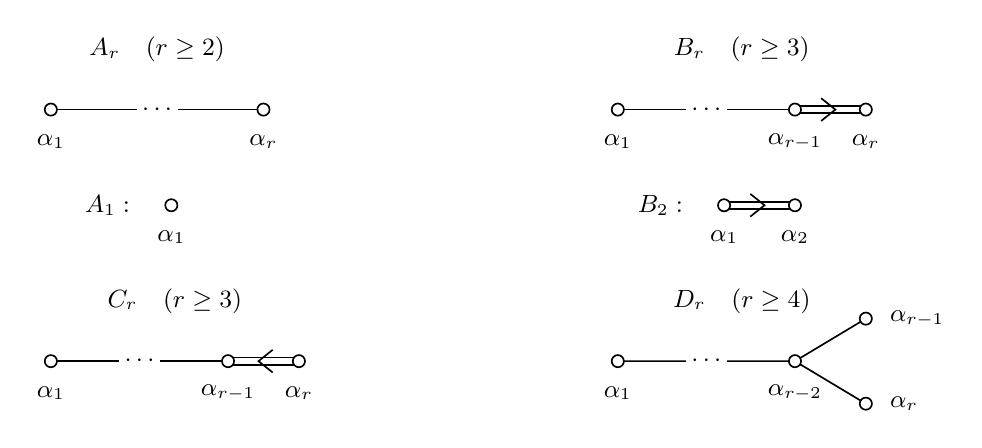
\begin{tikzpicture}[
  x=0.9cm,y=0.9cm,every node/.style={font=\small},
  every path/.style={line width=.6pt},
  root/.style={circle,draw,fill=white,inner sep=0pt,minimum size=4.4pt}]
  % A_r: the omitted single-edge chain may have no intermediate vertices.
  \node at (1.5,0.85) {\(A_r\quad(r\geq2)\)};
  \draw (0,0)--(3,0);
  \node[fill=white,inner sep=2pt] at (1.5,0) {\(\cdots\)};
  \node[root] at (0,0) {};
  \node[root] at (3,0) {};
  \node at (0,-0.45) {\(\alpha_1\)};
  \node at (3,-0.45) {\(\alpha_r\)};
  \node at (0.8,-1.35) {\(A_1:\)};
  \node[root] at (1.7,-1.35) {};
  \node at (1.7,-1.8) {\(\alpha_1\)};

  % B_r: alpha_r is short, so the double-edge arrow points right.
  \node at (9.75,0.85) {\(B_r\quad(r\geq3)\)};
  \draw (8,0)--(10.5,0);
  \node[fill=white,inner sep=2pt] at (9.25,0) {\(\cdots\)};
  \draw (10.5,0.05)--(11.5,0.05) (10.5,-0.05)--(11.5,-0.05);
  \draw (10.87,0.16)--(11.07,0)--(10.87,-0.16);
  \foreach \x in {8,10.5,11.5} \node[root] at (\x,0) {};
  \node at (8,-0.45) {\(\alpha_1\)};
  \node at (10.5,-0.45) {\(\alpha_{r-1}\)};
  \node at (11.5,-0.45) {\(\alpha_r\)};
  \node at (8.6,-1.35) {\(B_2:\)};
  \draw (9.5,-1.3)--(10.5,-1.3) (9.5,-1.4)--(10.5,-1.4);
  \draw (9.87,-1.19)--(10.07,-1.35)--(9.87,-1.51);
  \foreach \x in {9.5,10.5} \node[root] at (\x,-1.35) {};
  \node at (9.5,-1.8) {\(\alpha_1\)};
  \node at (10.5,-1.8) {\(\alpha_2\)};

  % C_r: alpha_r is long, so the double-edge arrow points left.
  \node at (1.75,-2.7) {\(C_r\quad(r\geq3)\)};
  \draw (0,-3.55)--(2.5,-3.55);
  \node[fill=white,inner sep=2pt] at (1.25,-3.55) {\(\cdots\)};
  \draw (2.5,-3.5)--(3.5,-3.5) (2.5,-3.6)--(3.5,-3.6);
  \draw (3.13,-3.39)--(2.93,-3.55)--(3.13,-3.71);
  \foreach \x in {0,2.5,3.5} \node[root] at (\x,-3.55) {};
  \node at (0,-4) {\(\alpha_1\)};
  \node at (2.5,-4) {\(\alpha_{r-1}\)};
  \node at (3.5,-4) {\(\alpha_r\)};

  % D_r: alpha_{r-2} is the fork; at r=4 the omitted chain is one edge.
  \node at (9.75,-2.7) {\(D_r\quad(r\geq4)\)};
  \draw (8,-3.55)--(10.5,-3.55)
    (10.5,-3.55)--(11.5,-2.95) (10.5,-3.55)--(11.5,-4.15);
  \node[fill=white,inner sep=2pt] at (9.25,-3.55) {\(\cdots\)};
  \foreach \x/\y in {8/-3.55,10.5/-3.55,11.5/-2.95,11.5/-4.15}
    \node[root] at (\x,\y) {};
  \node at (8,-4) {\(\alpha_1\)};
  \node at (10.5,-4) {\(\alpha_{r-2}\)};
  \node[anchor=west] at (11.7,-2.95) {\(\alpha_{r-1}\)};
  \node[anchor=west] at (11.7,-4.15) {\(\alpha_r\)};
\end{tikzpicture}
\caption[经典型 Dynkin 图]{经典型 Dynkin 图。省略号表示可含零个中间顶点的单边链段，根的编号沿链递增。
双边箭头指向短根；\(D_r\) 的分叉点为 \(\alpha_{r-2}\)。}
\label{b5:fig:classical-dynkin-diagrams}
\end{figure}

% !TeX root = ../Book5.tex
\begin{figure}[htbp]
\centering
\begin{tikzpicture}[
  x=0.9cm,y=0.9cm,every node/.style={font=\small},
  every path/.style={line width=.6pt},
  root/.style={circle,draw,fill=white,inner sep=0pt,minimum size=4.4pt}]
  % E_6, E_7, E_8 use the coordinate-model numbering; alpha_4 is the fork.
  \node at (2,2.05) {\(E_6\)};
  \draw (0,0)--(4,0) (2,0)--(2,1);
  \foreach \x/\i in {0/1,1/3,2/4,3/5,4/6} {
    \node[root] at (\x,0) {};
    \node at (\x,-0.45) {\(\alpha_\i\)};
  }
  \node[root] at (2,1) {};
  \node at (2,1.45) {\(\alpha_2\)};

  \node at (9.5,2.05) {\(E_7\)};
  \draw (7,0)--(12,0) (9,0)--(9,1);
  \foreach \x/\i in {7/1,8/3,9/4,10/5,11/6,12/7} {
    \node[root] at (\x,0) {};
    \node at (\x,-0.45) {\(\alpha_\i\)};
  }
  \node[root] at (9,1) {};
  \node at (9,1.45) {\(\alpha_2\)};

  \node at (6,-1.7) {\(E_8\)};
  \draw (3,-3.55)--(9,-3.55) (5,-3.55)--(5,-2.55);
  \foreach \x/\i in {3/1,4/3,5/4,6/5,7/6,8/7,9/8} {
    \node[root] at (\x,-3.55) {};
    \node at (\x,-4) {\(\alpha_\i\)};
  }
  \node[root] at (5,-2.55) {};
  \node at (5,-2.1) {\(\alpha_2\)};

  % F_4: alpha_1 and alpha_2 are long; alpha_3 and alpha_4 are short.
  \node at (1.5,-5.1) {\(F_4\)};
  \draw (0,-5.95)--(1,-5.95) (2,-5.95)--(3,-5.95);
  \draw (1,-5.9)--(2,-5.9) (1,-6)--(2,-6);
  \draw (1.37,-5.79)--(1.57,-5.95)--(1.37,-6.11);
  \foreach \x/\i in {0/1,1/2,2/3,3/4} {
    \node[root] at (\x,-5.95) {};
    \node at (\x,-6.4) {\(\alpha_\i\)};
  }

  % G_2: alpha_1 is short, so the triple-edge arrow points left.
  \node at (9.5,-5.1) {\(G_2\)};
  \draw (9,-5.89)--(10,-5.89) (9,-5.95)--(10,-5.95)
    (9,-6.01)--(10,-6.01);
  \draw (9.63,-5.77)--(9.43,-5.95)--(9.63,-6.13);
  \node[root] at (9,-5.95) {};
  \node[root] at (10,-5.95) {};
  \node at (9,-6.4) {\(\alpha_1\)};
  \node at (10,-6.4) {\(\alpha_2\)};
\end{tikzpicture}
\caption[例外型 Dynkin 图]{例外型 Dynkin 图。\(E_6,E_7,E_8\) 的分叉点均为 \(\alpha_4\)，
三个臂长分别为 \((1,2,2)\)、\((1,2,3)\)、\((1,2,4)\)；臂长计中心之外的顶点数。
\(F_4\) 的末两根短，\(G_2\) 的第一根短。}
\label{b5:fig:exceptional-dynkin-diagrams}
\end{figure}


分类时方便把每根归一到长度 \(\sqrt2\)。其 Gram 矩阵 \(G\) 满足
\[
G_{ii}=2,\qquad G_{ij}=-\sqrt{a_{ij}a_{ji}}\quad(i\ne j).
\]
这只是对 Gram 矩阵作正对角合同变换，仍然正定；它不把原来的长短根真的改成同一个根系。下一节通过这个正定矩阵限制图的形状，再用具体坐标验证所有剩下的图确实出现。

% !TeX root = ../../Book5.tex
% 纲要标题：### 17.3 根系分类
% 纲要位置：工作记录/计划纲要.md，第 4270 行。

\section{根系分类}
\label{b5:sec:1703}

本节先证明候选图形的穷尽性，再用坐标构造证明每种候选确实出现。两个步骤缺一不可：只画出经典图形不能排除其他图，只列出正定矩阵也没有自动给出根集合。

% 纲要要点已在下文展开。

% 纲要细目（保留原定写作范围）：
%
% * 不可约有限根系
% * 经典型与例外型
% * 低秩例子和同构
%

\subsection{不可约有限根系}
\label{b5:subsec:1703:01}

\begin{definition}\label{b5:def:irreducible-root-system}
设 \(\Phi\subseteq E\) 为非空有限约化结晶根系。若不能把它写成两个非空子集
\(\Phi_1,\Phi_2\) 的不交并，使两子集中的根两两正交，则称 \(\Phi\) 为\term{不可约根系}[irreducible root system]。
\end{definition}

Dynkin 图的连通分支与根系的正交不可约分支相对应。事实上，简单反射只在自己的图分支中改变坐标，每个根又都是简单根的反射像，故没有根跨越两个分支。于是分类只须处理连通图。

\begin{lemma}\label{b5:lem:finite-dynkin-list}
每个不可约有限约化结晶根系的 Dynkin 图，必为下列图形之一：
\[
A_r\ (r\geq1),\quad B_r\ (r\geq2),\quad C_r\ (r\geq3),\quad
D_r\ (r\geq4),\quad E_6,E_7,E_8,F_4,G_2.
\]
\end{lemma}
\begin{proof}
先证明图的穷尽性。使用上一节的正定矩阵 \(G\)，其对角元为 \(2\)，边上的负非对角元为 \(1,\sqrt2,\sqrt3\)。在非负向量上增大边权只会减小二次型，所以以下排除也适用于重边。

图不能有圈：在一个最短圈上赋值 \(1\)，其余为零，得到 \(x^{\mathsf T}Gx\leq0\)。一顶点不能有四个邻点：中心取 \(2\)，四邻点取 \(1\)，同样得到非正值。不能有两个三叉点：连接两点的路径全部取 \(2\)，两端各取两个外邻点赋值 \(1\)，其余为零；路径若有 \(l\) 个顶点，则在单边情形
\[
\frac12x^{\mathsf T}Gx=4l+4-4(l-1)-8=0.
\]
因此图为链，或只有一个三叉点的树。

消去叶点时改变的是剩余二次型。若叶点坐标为 \(t\)、其对角元为 \(d>0\)，其余坐标记为 \(x\)，配方得到
\[
dt^2+2t b^{\mathsf T}x+x^{\mathsf T}Ax
=d(t+d^{-1}b^{\mathsf T}x)^2+x^{\mathsf T}(A-bb^{\mathsf T}/d)x.
\]
叶点只与一个顶点相邻；若边权为 \(-\sqrt m\)，消去后这个邻点的对角元减少 \(m/d\)。原二次型正定，便要求剩下的 Schur 补仍正定。

若有三叉点，图不能有重边。取从三叉点到最近重边的路径，再保留三叉点另外两个方向各一个叶点，以及重边的另一端。对这个主子矩阵逐次消去叶点：两个单叶点各减去 \(1/2\)，使中心的有效对角元从 \(2\) 降为 \(1\)；沿路径的单边消元反复给出 \(2-1/1=1\)；最后重数 \(m\geq2\) 的边使终点对角元成为 \(2-m\leq0\)。这与正定矩阵的 Schur 补仍正定矛盾。

所以分叉情形全部为单边。设三个臂长为 \(p-1,q-1,r-1\)，其中
\(2\leq p\leq q\leq r\)。记 \(m_1=p,m_2=q,m_3=r\)，中心坐标为 \(t\)，
第 \(\nu\) 条臂的坐标为 \(x_{\nu,1},\ldots,x_{\nu,m_\nu-1}\)。补记
\(x_{\nu,0}=t,x_{\nu,m_\nu}=0\)，并令
\(z_{\nu,j}=x_{\nu,j}-(1-j/m_\nu)t\)，于是
\(z_{\nu,0}=z_{\nu,m_\nu}=0\)。逐臂配方得到
\[
\frac12x^{\mathsf T}Gx
=\frac12\sum_{\nu=1}^3\sum_{j=0}^{m_\nu-1}(z_{\nu,j}-z_{\nu,j+1})^2
+\frac12\left(\frac1p+\frac1q+\frac1r-1\right)t^2.
\]
正定性等价于三个倒数之和大于 \(1\)。若 \(p\geq3\)，和至多为 \(1\)，故 \(p=2\)；
若 \(q=2\)，所有 \(r\geq2\) 可行，得到 \(D_{r+2}\)；
若 \(q\geq4\)，仍不可能严格大于 \(1\)；剩下 \(q=3\)，只能
\(r=3,4,5\)，分别得到 \(E_6,E_7,E_8\)。

再处理链。链上至多有一条重边。否则取从第一条到下一条重边的最短子链，记两条重边的重数为 \(m,m'\geq2\)。正定性保证逐次消元所得的有效对角元都为正。
从首端消元后，第一条重边另一端的有效对角元为 \(2-m/2\leq1\)；沿中间单边消元时，若当前有效对角元为 \(0<d\leq1\)，下一个为 \(2-1/d\leq1\)，并仍须为正。
因此到达第二条重边前，其端点的有效对角元满足 \(0<d\leq1\)，最后一个 Schur 补对角元却为
\[
2-\frac{m'}d\leq2-m'\leq0,
\]
矛盾。三重边若还有一个相邻顶点，三阶主子式至多为
\(8-2\cdot3-2\cdot1=0\)，所以三重边只能单独构成 \(G_2\)。

若唯一重边为双边，设其两侧的单链分别有 \(p,q\) 个顶点，包含重边端点。
记有 \(p\) 个顶点的单链矩阵为 \(A_p\)，并约定 \(\det A_0=1\)。三对角行列式递推给出 \(\det A_p=p+1\)；逆矩阵的末端条目则由余子式公式得到
\[
(A_p^{-1})_{pp}=\frac{\det A_{p-1}}{\det A_p}=\frac p{p+1}.
\]
重边只连接两条单链的末端，所以对双边作 Schur 补，正定条件为
\[
1-\frac{2pq}{(p+1)(q+1)}>0,
\qquad\text{即}\qquad(p-1)(q-1)<2.
\]
交换两侧后设 \(p\leq q\)。于是或者 \(p=1\)，双边位于端部，按箭头方向得到 \(B_r,C_r\)；或者 \(p=q=2\)，得到 \(F_4\)。
没有重边的链为 \(A_r\)。这已经排除了所有其他形状；箭头方向由长度比决定，树上没有额外的相容性障碍。

这已经证明所列图形的穷尽性。
\end{proof}

上述证明与箭图中 ADE 正定型的分类有共同部分，但这里还处理了不等长根及重边。简单根 Gram 矩阵的正定性限制了 Dynkin 图可能的形状。

\subsection{经典型与例外型}
\label{b5:subsec:1703:02}

以下坐标均使用普通欧氏内积，只用于展示根系的形状。记 \(e_i\) 为标准正交基。四个经典族为
\begin{equation}\label{b5:eq:classical-root-models}
\begin{aligned}
A_r&:\ \{\,e_i-e_j\mid i\ne j,\ 1\leq i,j\leq r+1\,\}
\subseteq\{\textstyle\sum x_i=0\},\\
B_r&:\ \{\,\pm e_i,\ \pm e_i\pm e_j\mid i<j\,\},\\
C_r&:\ \{\,\pm2e_i,\ \pm e_i\pm e_j\mid i<j\,\},\\
D_r&:\ \{\,\pm e_i\pm e_j\mid i<j\,\}.
\end{aligned}
\end{equation}
两处正负号独立选取。\(A_r\) 取简单根 \(e_i-e_{i+1}\)；
\(B_r,C_r\) 前 \(r-1\) 个也如此，末根分别取 \(e_r,2e_r\)；
\(D_r\) 取 \(e_1-e_2,\ldots,e_{r-1}-e_r,e_{r-1}+e_r\)。
反射分别是坐标互换、改变一个坐标的符号，或互换两坐标并同时变号；
这些操作保持所列集合，结晶整数也由坐标立即读出。每个正根都能沿相邻差逐次展开，例如
\(e_i-e_j=\alpha_i+\cdots+\alpha_{j-1}\)；
对 \(i<j\)，和根在 \(B,C\) 型中分别展开为
\[
\begin{aligned}
B_r:\quad e_i+e_j&=\alpha_i+\cdots+\alpha_{j-1}
+2(\alpha_j+\cdots+\alpha_r),\\
C_r:\quad e_i+e_j&=\alpha_i+\cdots+\alpha_{j-1}
+2(\alpha_j+\cdots+\alpha_{r-1})+\alpha_r.
\end{aligned}
\]
差别来自末根分别为 \(e_r\) 与 \(2e_r\)。在 \(D_r\) 中，若 \(j<r\)，相应展开为
\[
e_i+e_j=\alpha_i+\cdots+\alpha_{j-1}
+2(\alpha_j+\cdots+\alpha_{r-2})+\alpha_{r-1}+\alpha_r;
\]
若 \(j=r\)，则为 \(e_i+e_r=\alpha_i+\cdots+\alpha_{r-2}+\alpha_r\)，其中空和为零。例如 \(D_4\) 中有 \(e_1+e_2=\alpha_1+2\alpha_2+\alpha_3+\alpha_4\)，两个分叉端共同补出和根。\(B_r\) 的短正根及 \(C_r\) 的长正根还分别满足 \(e_i=\alpha_i+\cdots+\alpha_r\)、\(2e_i=2(\alpha_i+\cdots+\alpha_{r-1})+\alpha_r\)。这些系数都非负。
因此所列根确为简单根，图分别是相应的链或分叉树。

\ProseParagraphBreak

例外型同样可以从有限坐标集合得到，毋须先构造例外 Lie 代数。
先取八维格
\[
L=\{\,z\in\mathbb Z^8\mid\textstyle\sum z_i\in2\mathbb Z\,\}
\ \cup\
\left(\frac12(1,\ldots,1)+
\{\,z\in\mathbb Z^8\mid\textstyle\sum z_i\in2\mathbb Z\,\}\right).
\]
它对加法封闭，所有向量的平方长度为偶整数，任意两个向量的内积为整数。
其中平方长度为 \(2\) 的向量恰为
\begin{equation}\label{b5:eq:e8-root-model}
\Phi_{E_8}=
\{\,\pm e_i\pm e_j\mid i<j\,\}
\ \cup\
\left\{\,\frac12(\pm e_1\pm\cdots\pm e_8)
\ \middle|\ \text{负号个数为偶数}\,\right\}.
\end{equation}
前一类有 \(112\) 个，后一类有 \(128\) 个。对任意这样的 \(\alpha\)，
\(s_\alpha(x)=x-(x,\alpha)\alpha\) 保持格 \(L\) 及长度，故保持这 \(240\) 个向量；
这也同时验证了反射与结晶公理。

\ProseParagraphBreak

取下列八个根：
\begin{equation}\label{b5:eq:e8-simple-roots}
\begin{aligned}
\alpha_1&=\tfrac12(e_1+e_8-e_2-e_3-e_4-e_5-e_6-e_7),&
\alpha_2&=e_1+e_2,\\
\alpha_3&=e_2-e_1,&
\alpha_4&=e_3-e_2,\\
\alpha_5&=e_4-e_3,&
\alpha_6&=e_5-e_4,\\
\alpha_7&=e_6-e_5,&
\alpha_8&=e_7-e_6.
\end{aligned}
\end{equation}
它们的图有中心 \(\alpha_4\)，三个臂长为 \(1,2,4\)。
还须验证它们确为简单根，不能只看图形。对 \(x=\sum c_i\alpha_i\in L\)，直接解坐标方程得到
\[
\begin{aligned}
c_1&=2x_8,&
c_2&=\tfrac12(x_1+x_2+\cdots+x_7+5x_8),\\
c_3&=\tfrac12(-x_1+x_2+\cdots+x_7+7x_8),&
c_4&=x_3+\cdots+x_7+5x_8,\\
c_5&=x_4+\cdots+x_7+4x_8,&
c_6&=x_5+x_6+x_7+3x_8,\\
c_7&=x_6+x_7+2x_8,&
c_8&=x_7+x_8.
\end{aligned}
\]
在 \(L\) 的两种陪集中，这些数都是整数。若一个平方长度为 \(2\) 的格向量同时有正、负系数，把它分成支集不交的非负组合 \(u-v\)。
不同简单根的内积非正，故 \((u,v)\leq0\)；两个非零格向量的平方长度至少为 \(2\)，遂有
\((u-v,u-v)\geq4\)，矛盾。
所以每个根的非零系数全为同一符号。定义
\[
\Phi^+=\left\{\,\alpha\in\Phi_{E_8}\ \middle|
\alpha=\sum_{i=1}^8c_i\alpha_i,\ c_i\geq0\,\right\}.
\]
八个 \(\alpha_i\) 是空间的一组基，故可取 \(v\) 使 \((v,\alpha_i)=1\) 对所有 \(i\) 成立。
于是 \((v,\alpha)=\sum_i c_i\)，每个根恰有一个符号属于 \(\Phi^+\)，而这正是由 \(v\) 选定的正根集合。
每个 \(\alpha_i\) 的系数向量是第 \(i\) 个单位向量，不能写成两个非零非负整数向量之和，因此不能写成两个正根之和。
由\cref{b5:thm:simple-roots}，全部简单正根构成空间的一组基；已经找到的八个 \(\alpha_i\) 因而就是这组简单根基。

\ProseParagraphBreak

在 \(\Phi_{E_8}\) 中分别取与 \(e_7+e_8\) 正交的根，以及同时与
\(e_7+e_8,e_6-e_7\) 正交的根，便得到 \(E_7,E_6\)。
与一个子空间相交所得的根集合对其中各根的反射封闭。上述坐标公式把 \(E_7\) 的条件写成 \(c_8=0\)，而 \(E_6\) 的两个条件写成 \(c_8=c_7=0\)；因此简单根分别为前七个和前六个 \(\alpha_i\)，并张成相应子空间。
对 \(E_7\)，整数根或者只用前六个坐标，或者为 \(\pm(e_7-e_8)\)，共有
\[
4\binom62+2=62
\]
个。半整数根的第七、八个符号必须相反；它们恰贡献一个负号，所以前六个符号中的负号数必须为奇数，共有 \(2\cdot2^5=64\) 种。

\ProseParagraphBreak

对 \(E_6\)，还须有 \(x_6=x_7=-x_8\)。整数根只有两个非零坐标，因此后三个坐标均为零，共有 \(4\binom52=40\) 个。
半整数根的后三个符号满足 \(\varepsilon_6=\varepsilon_7=-\varepsilon_8\)，只有两种选法；每种选法都要求前五个符号满足一个指定的负号奇偶条件，共有 \(2\cdot2^4=32\) 个。
所以 \(E_7\) 有 \(62+64=126\) 个根，\(E_6\) 有 \(40+32=72\) 个根。
这样也核验了三个例外图的存在，而非仅仅列出符号。

\ProseParagraphBreak

\(F_4\) 的根集合为
\[
\{\,\pm e_i,\ \pm e_i\pm e_j\mid i<j\,\}
\ \cup\
\left\{\,\tfrac12(\pm e_1\pm e_2\pm e_3\pm e_4)\,\right\},
\]
共有 \(48\) 个根，取简单根
\[
e_2-e_3,\quad e_3-e_4,\quad e_4,\quad
\tfrac12(e_1-e_2-e_3-e_4).
\]
符号改变与坐标置换显然保持根集合；剩下只须检验关于
\(\tfrac12(e_1+e_2+e_3+e_4)\) 的反射。
它把坐标短根变成半整数短根，把两坐标同号的长根变成另外两坐标的长根，
保持两坐标异号的长根；对半整数短根，按负号数 \(0,1,2,3,4\) 逐项代入，分别得到半整数根、坐标根、原根、坐标根、半整数根。
因此反射公理成立，配对的整数性也由这些同类计算给出。
若 \(x=\sum c_i\alpha_i\)，则
\[
c_4=2x_1,\quad c_1=x_1+x_2,\quad
c_2=2x_1+x_2+x_3,\quad c_3=3x_1+x_2+x_3+x_4.
\]
对所列三类根，按第一个非零坐标的符号检查，系数全为同号整数；
这证明四根构成简单根基，图中间为双边。

\ProseParagraphBreak

\(G_2\) 在 \(\sum x_i=0\) 的三维坐标平面中取
\[
\bigl\{\,\pm(e_i-e_j)\mid i<j\,\bigr\}
\ \cup\
\bigl\{\,\pm(2e_i-e_j-e_k)\mid\{i,j,k\}=\{1,2,3\}\,\bigr\}.
\]
简单根可取 \(\alpha_1=e_1-e_2\)、\(\alpha_2=-2e_1+e_2+e_3\)，正根为
\[
\alpha_1,\ \alpha_2,\ \alpha_1+\alpha_2,\
2\alpha_1+\alpha_2,\ 3\alpha_1+\alpha_2,\
3\alpha_1+2\alpha_2.
\]
两简单反射在坐标 \((a,b)\) 上分别作用为
\((a,b)\mapsto(-a+3b,b)\)、\((a,b)\mapsto(a,a-b)\)。
它们置换上述六个根及其负根，并把每个根变到一个简单根；
故关于任意根的反射也是这两个反射的共轭，四条根系公理随之成立。

设 \(\Phi\subseteq E\)、\(\Phi'\subseteq E'\) 为有限约化结晶根系，两个空间分别带有内积 \((\ ,\ )\)、\((\ ,\ )'\)。若线性双射 \(u:E\to E'\) 满足 \(u(\Phi)=\Phi'\)，并保持全部 Cartan 整数，即
\[
\frac{2(u\beta,u\alpha)'}{(u\alpha,u\alpha)'}
=\frac{2(\beta,\alpha)}{(\alpha,\alpha)}
\qquad(\alpha,\beta\in\Phi),
\]
则称 \(u\) 为根系同构。由\cref{b5:prop:cartan-determines-roots}，对这样的根集合双射，保持 Cartan 整数等价于在每个不可约分支上将内积乘以一个正数；不同分支可以采用不同的比例。

\begin{theorem}[根系分类]\label{b5:thm:root-classification}
不可约有限约化结晶根系的同构类型恰为
\(A_r\ (r\geq1)\)、\(B_r\ (r\geq2)\)、\(C_r\ (r\geq3)\)、
\(D_r\ (r\geq4)\)、\(E_6,E_7,E_8,F_4,G_2\)。
任意有限约化结晶根系唯一分成这些类型的正交直和，忽略分支的排列次序。
\end{theorem}
\begin{proof}
\cref{b5:lem:finite-dynkin-list}排除了全部其他图。
本小节逐一给出的坐标集合满足根系公理，并已检查简单根及 Dynkin 图，所以每种图均存在。
\cref{b5:prop:cartan-determines-roots}说明相同的带箭头图确定根集合，长度只差整体正比例。
最后，图的连通分支恰好给出根系的正交不可约分支，且图的连通分解唯一。
\end{proof}

\subsection{低秩例子和同构}
\label{b5:subsec:1703:03}

上述参数范围去掉了低秩重复。\(B_1,C_1\) 都给出 \(A_1\)；
\(B_2\) 与 \(C_2\) 通过平面旋转及整体缩放同构；
\(D_3\) 的分叉退化为 \(A_3\)，而 \(D_2=A_1\oplus A_1\) 可约。
秩至少为 \(3\) 时，\(B_r\) 与 \(C_r\) 的长短根数量相反，不能再通过整体相似互换。
它们的 Weyl 群却相同，都是全部带符号的坐标置换群。这说明 Weyl 群本身并不确定根系。

\begin{proposition}\label{b5:prop:root-components-simple-ideals}
设 \(\mathfrak g\) 为有限维复半单 Lie 代数，\(\mathfrak h\subseteq\mathfrak g\) 为 Cartan 子代数，\(\Phi\) 为相应根系。记 \(\mathfrak g_\alpha\) 为根空间，\(t_\alpha\in\mathfrak h\) 为满足 \(\kappa_{\mathfrak g}(t_\alpha,h)=\alpha(h)\) 对所有 \(h\in\mathfrak h\) 成立的元素。\(\Phi\) 的不可约分支与 \(\mathfrak g\) 的单理想一一对应；对应于分支 \(\Psi\subseteq\Phi\) 的理想为
\[
\mathfrak g(\Psi)
=\operatorname{span}_{\mathbb C}\{\,t_\alpha\mid\alpha\in\Psi\,\}
\oplus\bigoplus_{\alpha\in\Psi}\mathfrak g_\alpha.
\]
\end{proposition}
\begin{proof}
不同根系分支正交，且不存在跨分支的根和。根空间括号公式及
\([t_\alpha,\mathfrak g_\beta]=\beta(t_\alpha)\mathfrak g_\beta\)
说明不同的 \(\mathfrak g(\Psi)\) 互相交换，且各自为理想，其直和为 \(\mathfrak g\)。
另一方面，\cref{b5:thm:semisimple-ideal-decomposition}将 \(\mathfrak g\) 分成单理想。
先在各单理想中取 Cartan 子代数；它们之和自中心化且为环面，故是 \(\mathfrak g\) 的 Cartan 子代数。
不同单理想的根互相正交；一个单理想的根系若可分解，前一段的构造又会把该理想分成两个非零理想，矛盾。
最后用\cref{b5:thm:cartan-conjugacy}把这份 Cartan 子代数搬到当前 \(\mathfrak h\)，所以每个不可约分支恰对应一个单理想。
\end{proof}

正交矩阵模型可在复数域上改用双曲基，此时偶维对称型的矩阵为 \(J=\left(\begin{smallmatrix}0&I_r\\I_r&0\end{smallmatrix}\right)\)，条件是 \(X^{\mathsf T}J+JX=0\)。这样的矩阵写成
\[
X=\begin{pmatrix}A&B\\C&-A^{\mathsf T}\end{pmatrix},
\qquad B^{\mathsf T}=-B,\quad C^{\mathsf T}=-C.
\]
取 \(\mathfrak h=\{\operatorname{diag}(t_1,\ldots,t_r,-t_1,\ldots,-t_r)\}\)，并令 \(\varepsilon_i(H)=t_i\)。以 \(E_{ab}\) 记矩阵单位，代表性的根向量为
\[
\begin{aligned}
E_{ij}-E_{r+j,r+i}&:\ \varepsilon_i-\varepsilon_j\quad(i\ne j),\\
E_{i,r+j}-E_{j,r+i}&:\ \varepsilon_i+\varepsilon_j\quad(i<j),\\
E_{r+i,j}-E_{r+j,i}&:\ -\varepsilon_i-\varepsilon_j\quad(i<j).
\end{aligned}
\]
这里用 \([H,E_{ab}]=(H_{aa}-H_{bb})E_{ab}\) 即可逐项检验。\(B,C\) 的对角元为零，排除了 \(\pm2\varepsilon_i\)；零权空间恰是 \(\mathfrak h\)，故它是 Cartan 子代数，得到 \(D_r\) 的根。

\ProseParagraphBreak
奇维时把型的矩阵取成 \(\operatorname{diag}(J,1)\)，给 \(H\) 添一个末坐标 \(0\)，并以 \(o=2r+1\) 记这个坐标。除上述根向量外，还有
\[
E_{i,o}-E_{o,r+i}:\ \varepsilon_i,
\qquad E_{r+i,o}-E_{o,i}:\ -\varepsilon_i.
\]
它们满足同一个正交条件，给出 \(B_r\) 额外的短根。这种基变换说明为何标准模型 \(X^{\mathsf T}+X=0\) 中不显眼的对角 Cartan 子代数，在双曲基中可以直接写出。

\ProseParagraphBreak
经典根系由
\(\mathfrak{sl}_{r+1}\)、\(\mathfrak{so}_{2r+1}\)、\(\mathfrak{sp}_{2r}\)、
\(\mathfrak{so}_{2r}\) 实现。例外型也将由下一节的统一展示构造得到。
例如 \(G_2,F_4\) 另有与八元数代数、Albert 代数\footnote{艾伯特（Abraham Adrian Albert，1905-1972），美国数学家，研究非结合代数与中心单代数；例外型 Jordan 代数以他命名。}的导子有关的具体模型。这些模型的构造涉及额外的非结合代数理论。

% !TeX root = ../../Book5.tex
% 纲要标题：### 17.4* 从根系到 Lie 代数
% 纲要位置：工作记录/计划纲要.md，第 4276 行。

\OptionalSection{从根系到 Lie 代数}{b5:sec:1704}

有限根系的分类已经完成，本节补足由根系恢复复半单 Lie 代数的构造。对一个已经给定的半单 Lie 代数研究表示时，不以这个存在性构造为前提。

% 纲要要点已在下文展开。

% 纲要细目（保留原定写作范围）：
%
% * Serre 关系与呈示
% * 复半单 Lie 代数分类的存在和唯一性问题
% * 区分根系分类的正文证明与完整呈示构造的选读证明
%
% ---
%

\subsection{Serre 关系与呈示}
\label{b5:subsec:1704:01}

根系分类给出有限的图表，却还留下两个代数问题：每个图是否来自一个 Lie 代数；同一个图是否只能来自一个同构类型。本节同时解决二者。证明只使用已建立的根系、自由代数及根 \(\mathfrak{sl}_2\) 计算，不借用下一章的最高权分类。生成关系、自由字模型及局部幂零反射的证明方法可对照\cite[Sections 18.1--18.4, pp. 96--101]{Humphreys1972LieAlgebras}。

\begin{definition}\label{b5:def:serre-algebra}
设 \(A=(a_{ij})\in M_r(\mathbb Z)\) 是有限约化结晶根系的 Cartan 矩阵，行对应余根。取复自由 Lie 代数的生成元
\(e_i,f_i,h_i\)（\(1\leq i\leq r\)），并加上下列关系：
\begin{equation}\label{b5:eq:serre-relations}
\begin{aligned}
[h_i,h_j]&=0,&
[h_i,e_j]&=a_{ij}e_j,&
[h_i,f_j]&=-a_{ij}f_j,\\
[e_i,f_j]&=\delta_{ij}h_i,&
(\operatorname{ad}e_i)^{1-a_{ij}}e_j&=0,&
(\operatorname{ad}f_i)^{1-a_{ij}}f_j&=0\quad(i\ne j).
\end{aligned}
\end{equation}
由自由 Lie 代数模去这些关系生成的理想所得的 Lie 代数记为
\(\mathfrak g(A)\)。这组关系称为\term{Serre 关系}[Serre relations]，给出 \(\mathfrak g(A)\) 的生成元与关系展示。
\end{definition}

自由 Lie 代数可以不借助存在性定理而直接构造：对生成元的所有有限带括号字取自由向量空间，把反对称性和 Jacobi 恒等式生成的理想模掉；每个到某个 Lie 代数的生成元映射唯一延拓为同态。这一泛性质保证上述商的含义明确。

\ProseParagraphBreak

给出生成元和关系之后，还须证明所得代数非零，并证明 \(h_i\) 线性无关。下面构造一个允许任意复参数的具体作用来证明这两点。

\begin{lemma}\label{b5:lem:serre-triangular-noncollapse}
设 \(\Phi\) 为有限约化结晶根系，\(\{\alpha_1,\ldots,\alpha_r\}\) 为简单根基，\(A\in M_r(\mathbb Z)\) 为相应有限型 Cartan 矩阵。记 \(\mathfrak g(A)\) 为由复生成元 \(e_i,f_i,h_i\) 及 Serre 关系\eqref{b5:eq:serre-relations}定义的 Lie 代数。令 \(\mathfrak n^\pm\) 为
\(\mathfrak g(A)\) 中由 \(e_i\)、\(f_i\) 分别生成的子代数，令
\(\mathfrak h=\sum_i\mathbb Ch_i\)。则
\[
\mathfrak g(A)=\mathfrak n^-\oplus\mathfrak h\oplus\mathfrak n^+,
\]
且 \(h_1,\ldots,h_r\) 线性无关。按照
\(\deg e_i=\alpha_i,\deg f_i=-\alpha_i,\deg h_i=0\)，这个代数有根格分次；
非零次数只能是简单根的全非负组合或全非正组合。
\end{lemma}
\begin{proof}
先在自由结合代数 \(T=\mathbb C\langle f_1,\ldots,f_r\rangle\) 上构造算子。
给定任意参数 \(\lambda_1,\ldots,\lambda_r\)，令 \(F_i\) 为左乘 \(f_i\)；
对次数为 \(-\beta=-\sum_jn_j\alpha_j\) 的字 \(u\)，令
\[
H_i u=\left(\lambda_i-\sum_jn_ja_{ij}\right)u.
\]
再按字长递归规定
\[
E_i1=0,\qquad E_i(f_j u)=f_jE_i u+\delta_{ij}H_i u.
\]
由此直接得到
\([H_i,H_j]=0\)、\([H_i,F_j]=-a_{ij}F_j\)、
\([H_i,E_j]=a_{ij}E_j\)、\([E_i,F_j]=\delta_{ij}H_i\)。
例如第三式可在 \(1\) 上验证后，把两边作用于 \(f_k u\)，利用递归式把差化为相同关系在较短字 \(u\) 上的差。

令 \(J\) 为由
\(S_{ij}=(\operatorname{ad}f_i)^{1-a_{ij}}f_j\)（\(i\ne j\)）
生成的双边理想。它是齐次的，故被各 \(H_k\) 保持，也被左乘保持。
还须验证各 \(E_k\) 保持它。对 \(m=1-a_{ij}\)，交换子法则及上面的四组关系给出
\[
\bigl[E_i,(\operatorname{ad}F_i)^mF_j\bigr]
=m(-a_{ij}-m+1)(\operatorname{ad}F_i)^{m-1}F_j=0.
\]
当 \(k\ne i,j\) 时交换子为零；当 \(k=j\) 时，结果为
\((\operatorname{ad}F_i)^mH_j\)，也为零：
若 \(m\geq2\)，第二次括号已经消失；若 \(m=1\)，则 \(a_{ij}=a_{ji}=0\)。
因此 \(E_k(S_{ij}u)=S_{ij}E_ku\)。在左侧再逐个添 \(f_l\)，递归式说明新产生的 \(H_k\) 项仍在齐次理想 \(J\) 中。故 \(E_kJ\subseteq J\)。

这些算子于是降到非零空间 \(T/J\) 上；它非零是因为 \(J\) 由正次数齐次元生成，不含 \(1\)。
负 Serre 关系按构造成立。正 Serre 算子
\(R_{ij}=(\operatorname{ad}E_i)^{1-a_{ij}}E_j\)
与每个 \(F_k\) 交换：交换前一段的 \(E,F\) 并把 \(H\) 改成 \(-H\)，所得同一个系数恰为零。又因 \(E_i1=0\)，有 \(R_{ij}1=0\)，故与全部左乘交换后，\(R_{ij}\) 在每个字上都为零。
所以这确实是 \(\mathfrak g(A)\) 的作用。
若 \(\sum c_i h_i=0\)，作用在 \(1\) 上得到
\(\sum c_i\lambda_i=0\) 对所有复参数成立，故每个 \(c_i=0\)。

最后证明三角跨度。由 Jacobi 恒等式及
\([e_i,f_j]=\delta_{ij}h_i\)，有
\([e_i,\mathfrak n^-]\subseteq\mathfrak n^-+\mathfrak h\)：
对负字长度归纳，括号经过一个 \(f_j\) 后或者留下较短负字，或者成为 \(h_i\)，后者再与其余负字作括号仍回到 \(\mathfrak n^-\)。
同理 \([f_i,\mathfrak n^+]\subseteq\mathfrak n^++\mathfrak h\)。
继续对正字长度归纳，得到
\([\mathfrak n^+,\mathfrak n^-]\subseteq
\mathfrak n^-+\mathfrak h+\mathfrak n^+\)。
故该和是含全部生成元的子代数，等于 \(\mathfrak g(A)\)。
所有关系齐次，所以根格分次下降到商；正次数、零次数、负次数互不相交，和因此为直和。次数为 \(\alpha_i\) 的空间至多一维，由 \(e_i\) 张成；负简单次数同理。
\end{proof}

\subsection{复半单 Lie 代数的存在性与唯一性}
\label{b5:subsec:1704:02}

\begin{theorem}[Serre 展示]\label{b5:thm:serre-presentation}
设 \(\Phi\) 为秩 \(r\) 的有限约化结晶根系，\(A\in M_r(\mathbb Z)\) 为相应简单根基下的 Cartan 矩阵。记 \(\mathfrak g(A)\) 为复生成元 \(e_i,f_i,h_i\)（\(1\le i\le r\)）及 Serre 关系
\eqref{b5:eq:serre-relations}定义的 Lie 代数。则 \(\mathfrak g(A)\) 是有限维复半单 Lie 代数，
\(\mathfrak h=\bigoplus_i\mathbb Ch_i\) 是其 Cartan 子代数，其根系与 \(\Phi\) 同构，并且
\[
\dim\mathfrak g(A)=r+|\Phi|.
\]
任意具有根系 \(\Phi\) 的有限维复半单 Lie 代数，都同构于 \(\mathfrak g(A)\)。
\end{theorem}
\begin{proof}
先证有限维，不能把它当作展示的当然结果。导子
\(\operatorname{ad}e_i,\operatorname{ad}f_i\) 在每个生成元上局部幂零：
对同号生成元是 Serre 关系，对异号生成元和 \(h_j\) 则由前三组关系直接算出。
若导子在两个元素上分别由某次幂零化，二项式法则说明它也在二者的括号上由某次幂零化；因此它们在整个 \(\mathfrak g(A)\) 上局部幂零。
于是
\[
T_i=\exp(\operatorname{ad}e_i)
\exp(-\operatorname{ad}f_i)
\exp(\operatorname{ad}e_i)
\]
逐元素由有限和定义，是自同构。标准三元组计算给出
\(T_i(h_j)=h_j-a_{ji}h_i\)；所以 \(T_i\) 把次数为 \(\beta\) 的空间同构地送到次数为 \(s_i\beta\) 的空间。这里 \(A\) 可逆，根格的次数由全部 \(h_j\) 特征值唯一确定。

若正次数 \(\beta=\sum n_i\alpha_i\ne0\) 的空间非零，则
\((\beta,\beta)=\sum n_i(\beta,\alpha_i)>0\)，可选 \(i\) 使
\(\beta(h_i)=2(\beta,\alpha_i)/(\alpha_i,\alpha_i)>0\)。
若 \(\beta\) 有其他非零系数，\(s_i\beta\) 仍有这些正系数；三角分次排除了混合正负系数，故 \(s_i\beta\) 全非负，而高度严格减少。
若 \(\beta\) 只支持在 \(i\)，则对应正字只能由 \(e_i\) 自己组成；一个元素与自己作括号为零，所以只能有 \(\beta=\alpha_i\)。
迭代降高度，得每个非零次数都可由简单反射变成简单根或其负根。
因此所有次数都属于有限集合 \(W\Delta=\Phi\)，每个次数空间至多一维。
这已经证明 \(\dim\mathfrak g(A)\leq r+|\Phi|\)。

由上一引理 \(h_i\ne0\)，而 \([e_i,f_i]=h_i\)，所以 \(e_i,f_i\ne0\)。
再用 \(T_i\)，全部 \(\Phi\) 次数空间都非零，维数恰为一；
于是维数等式成立。各 \(\operatorname{ad}h_i\) 在这个有限分次上同时对角化，零权空间恰为 \(\mathfrak h\)，故 \(\mathfrak h\) 自中心化。

接着证明半单性。在 \(\mathfrak h\) 上，Killing 型为
\[
B_A(h,k)=\sum_{\alpha\in\Phi}\alpha(h)\alpha(k).
\]
对实线性生成空间 \(\sum_i\mathbb Rh_i\)，它正定，因为 Cartan 矩阵可逆、根分离点。因此 \(B_A|_{\mathfrak h}\) 非退化。
每个根次数经某个 \(T_i\) 乘积移到简单根次数，相应三元组也由自同构搬过去。对简单三元组，不变性给出
\[
2B_A(e_i,f_i)=B_A(h_i,h_i)\ne0.
\]
所以每对相反根空间的配对都非退化。不同且不相反的权空间互相正交，故整个 \(B_A\) 非退化。\cref{b5:thm:killing-semisimple}遂给出半单性；自中心化的环面 \(\mathfrak h\) 极大，正是 Cartan 子代数。

最后设 \(\mathfrak g\) 为具有根系 \(\Phi\) 的复半单 Lie 代数。
在简单根空间中选择标准三元组 \(e_i,f_i,h_i\)。
不同简单根之差不是根，给出 \([e_i,f_j]=0\)（\(i\ne j\)）；
根弦定理说明
\((\operatorname{ad}e_i)^{1-a_{ij}}e_j=0\)，负根同理。
其余关系由三元组和权直接成立。因此得到
\(\mathfrak g(A)\to\mathfrak g\) 的同态。
\cref{b5:prop:root-bracket-generation}说明像含有 \(\mathfrak h\) 及全部根空间，所以满射。
两边均有维数 \(r+|\Phi|\)，故核为零，这便证明唯一性。
\end{proof}

\subsection{根系分类与 Lie 代数呈示}
\label{b5:subsec:1704:03}

\secref{b5:sec:1703}以正定性确定可能的 Dynkin 图，并逐一构造相应根系。
本节的 Serre 展示进一步构造 Lie 括号，证明每个有限型 Cartan 矩阵都对应一个半单 Lie 代数，其维数为秩与根数之和，而且同图的复半单 Lie 代数彼此同构。

\ProseParagraphBreak

由\cref{b5:prop:root-components-simple-ideals}，连通图对应单 Lie 代数。
因此复单 Lie 代数分成四个经典族和五个例外型。例外型的维数由根数加秩得到：
\[
\begin{gathered}
\dim E_6=78,\qquad \dim E_7=133,\qquad \dim E_8=248,\\
\dim F_4=52,\qquad \dim G_2=14.
\end{gathered}
\]
这里的 \(E_6\) 等符号在语境明确时兼指根系型或相应单 Lie 代数；
写维数时指后者。分类按复 Lie 代数同构进行，不能据此把不同的实形式、不同中心的 Lie 群或正特征 Lie 代数也视为同一个分类问题。


\begin{chaptersummary}
Weyl 群由简单反射生成，最短表达的长度等于它改变符号的正根数。室的内部具有单纯传递作用，闭室则给每个轨道唯一代表；位于边界上的向量仍可有非平凡稳定子群。权格采用简单余根的对偶基，支配整权因而对应基本权的非负整数系数。

\ProseParagraphBreak

Dynkin 图保存 Cartan 矩阵，Cartan 矩阵再通过简单反射恢复全部根。分类的穷尽性来自正定 Gram 矩阵：先排除圈和复杂分叉，再对三臂树与含重边的链逐一计算。坐标模型保证留下的每一种形状都确实存在。

\ProseParagraphBreak

Serre 构造从 Dynkin 图得到 Lie 代数。允许任意参数的自由字作用证明 Cartan 生成元线性无关；局部幂零的伴随指数把可能的非零次数降到简单根；有限根集合随后给出整个代数的维数。存在性与唯一性的证明只使用此前建立的结果，无须最高权表示分类。
\end{chaptersummary}

\BookExercises

\begin{exercise}\label{b5:ex:17-s4-length}
在 \(A_3\) 中取标准正根 \(e_i-e_j\)（\(i<j\)）。
对排列 \(w=[3,1,4,2]\)，求 \(\ell(w)\)，并给出最短相邻交换表达。
\end{exercise}
\begin{solution}
逆序对为 \((1,2),(1,4),(3,4)\)，故长度为 \(3\)。
采用右侧先作用的约定，
\(w=s_2s_1s_3\)：它依次把 \(1,2,3,4\) 送到 \(3,1,4,2\)。
这个三因子表达达到逆序数下界，所以最短。
\end{solution}

\begin{exercise}\label{b5:ex:17-b2-weyl}
在 \(B_2\) 中取 \(\alpha_1=e_1-e_2,\alpha_2=e_2\)。
写出简单反射矩阵，求 \(s_1s_2\) 的阶和 \(W\) 的阶。
\end{exercise}
\begin{solution}
\[
s_1=\begin{pmatrix}0&1\\1&0\end{pmatrix},\qquad
s_2=\begin{pmatrix}1&0\\0&-1\end{pmatrix},\qquad
s_1s_2=\begin{pmatrix}0&-1\\1&0\end{pmatrix}.
\]
乘积是直角旋转，阶为 \(4\)。坐标互换及一个坐标变号生成全部带符号置换，
共有 \(2^2\cdot2!=8\) 个，故 \(W\) 为八阶二面体群。
\end{solution}

\begin{exercise}\label{b5:ex:17-classical-weyl}
由根反射的坐标公式证明：
\(W(B_r)=W(C_r)\) 是全部带符号置换群，
\(W(D_r)\) 是变号次数为偶数的带符号置换群。求它们的阶。
\end{exercise}
\begin{solution}
\(e_i-e_j\) 的反射交换两个坐标；
\(e_i\) 或 \(2e_i\) 的反射改变一个坐标的符号，故前两类生成全部带符号置换，阶为 \(2^r r!\)。
\(D_r\) 只有和根、差根；和根的反射在互换坐标的同时改变这两个符号，故总变号数为偶数。
结合普通坐标互换，可以实现任意两坐标同时变号，因此得到全部偶变号置换，阶为 \(2^{r-1}r!\)。
\end{solution}

\begin{exercise}\label{b5:ex:17-a2-weight}
对 \(A_2\) 的
\(\alpha_1=e_1-e_2,\alpha_2=e_2-e_3\)，求基本权，并证明
\(P/Q\cong\mathbb Z/3\mathbb Z\)。
\end{exercise}
\begin{solution}
解与两简单余根的配对方程及坐标和为零的条件，得
\[
\omega_1=\tfrac13(2,-1,-1),\qquad
\omega_2=\tfrac13(1,1,-2).
\]
根为
\(\alpha_1=2\omega_1-\omega_2,\alpha_2=-\omega_1+2\omega_2\)。
模根格后有 \(\omega_2=2\omega_1\)、\(3\omega_1=0\)；
而 \(\omega_1\) 的坐标不是整数，所以不在 \(Q\) 中。故商恰为三阶循环群。
\end{solution}

\begin{exercise}\label{b5:ex:17-b2-weights}
对 \(B_2\) 的上述简单根，求 \(Q,P\) 和基本权，判断 \(e_1/2\) 是否为整权。
\end{exercise}
\begin{solution}
简单余根为 \(e_1-e_2,2e_2\)，故
\(\omega_1=e_1,\omega_2=(e_1+e_2)/2\)。
有 \(Q=\mathbb Z^2\)，而
\[
P=\mathbb Z^2\cup
\left(\tfrac12(e_1+e_2)+\mathbb Z^2\right).
\]
\(e_1/2\) 与第一简单余根的配对为 \(1/2\)，所以不是整权。
只有同时出现的两个半整数坐标才属于另一陪集。
\end{solution}

\begin{exercise}\label{b5:ex:17-dominant-representative}
在 \(A_2\) 中求权 \(\lambda=-\omega_1+2\omega_2\) 的支配代表，
并列出它与这个代表之差。
\end{exercise}
\begin{solution}
\(\lambda=(0,1,-1)\)。按坐标递减排列，支配代表为
\((1,0,-1)=\omega_1+\omega_2\)，由交换前两坐标得到。
代表减原权为 \((1,-1,0)=\alpha_1\)。
所以原权虽是一个正根，却不是支配权；“正根”与“支配”采用不同判断条件。
\end{solution}

\begin{exercise}\label{b5:ex:17-boundary-stabilizer}
在 \(A_3\) 的闭基本室中，取
\(\mu=(2,2,-1,-3)\)。求它的 Weyl 稳定子群及轨道大小，并解释与 Weyl 室上单纯传递作用的区别。
\end{exercise}
\begin{solution}
只有前两个坐标相等，所以稳定子群由交换它们的 \(s_1\) 生成，阶为 \(2\)；
轨道大小为 \(4!/2=12\)。
\(\mu\) 在墙 \((\mu,\alpha_1)=0\) 上，不属于任何开室。群在室的集合上单纯传递，并不要求每个边界向量的稳定子群都平凡。
\end{solution}

\begin{exercise}\label{b5:ex:17-rho-a}
在 \(A_{r}\) 中求 \(\rho\) 的标准坐标，并验证每两个相邻坐标之差为 \(1\)。
\end{exercise}
\begin{solution}
坐标 \(e_i\) 在正根和中正出现 \(r+1-i\) 次，负出现 \(i-1\) 次，所以
\[
\rho=\frac12\sum_{i=1}^{r+1}(r+2-2i)e_i.
\]
第 \(i\) 与第 \(i+1\) 个坐标之差为 \(1\)，故与每个简单余根的配对为 \(1\)。
坐标和为零，确实属于根空间。
\end{solution}

\begin{exercise}\label{b5:ex:17-cartan-arrows}
矩阵
\(A=\left(\begin{smallmatrix}2&-1\\-3&2\end{smallmatrix}\right)\)
采用本书的行余根约定。判断根的长短、长度平方之比和 Dynkin 箭头方向。
\end{exercise}
\begin{solution}
由对称性
\((\alpha_1,\alpha_1)a_{12}=(\alpha_2,\alpha_2)a_{21}\)，得
\((\alpha_1,\alpha_1)=3(\alpha_2,\alpha_2)\)。
因此第一根长、第二根短，画三重边并将箭头指向第二根。这是 \(G_2\) 的另一编号次序。
\end{solution}

\begin{exercise}\label{b5:ex:17-cartan-index}
设 \(A\) 为秩 \(r\) 根系的 Cartan 矩阵。证明
\([P:Q]=|\det A|\)，并算出 \(A_r\) 的这个指数。
\end{exercise}
\begin{solution}
由 \(\alpha_j=\sum_i a_{ij}\omega_i\)，根格在基本权坐标中就是
\(A\mathbb Z^r\)。整数矩阵的 Smith 标准形说明其指数等于非零不变因子的乘积，即 \(|\det A|\)。
\(A_r\) 的三对角行列式 \(d_r\) 满足
\(d_r=2d_{r-1}-d_{r-2}\)、\(d_0=1,d_1=2\)，故 \(d_r=r+1\)。
\end{solution}

\begin{exercise}\label{b5:ex:17-three-arm-obstruction}
构造三臂长为 \(2,2,2\) 的单边树的一个正整数零向量，即使其 Gram 二次型为零的非零向量。若在任一臂上再加一个顶点，为什么仍不可能正定？
\end{exercise}
\begin{solution}
中心赋值 \(3\)，每条臂从中心向外赋值 \(2,1\)。
半个 Gram 二次型等于
\(9+3(4+1)-3(6+2)=0\)。
加顶点后让新坐标为零，原向量的二次型仍为零，因此扩大的矩阵仍非正定。
这也说明分类中三臂倒数和必须严格大于 \(1\)。
\end{solution}

\begin{exercise}\label{b5:ex:17-two-double-obstruction}
对三个顶点、两条边都为双边的链，写出归一 Gram 矩阵并找出非零零向量。
\end{exercise}
\begin{solution}
\[
G=\begin{pmatrix}2&-\sqrt2&0\\-\sqrt2&2&-\sqrt2\\0&-\sqrt2&2\end{pmatrix},
\qquad
G(1,\sqrt2,1)^{\mathsf T}=0.
\]
因此这种链不能是有限根系的 Dynkin 图。仅有每条边的重数不超过三，并不足以保证正定性。
\end{solution}

\begin{exercise}\label{b5:ex:17-classical-count}
数出 \(A_r,B_r,C_r,D_r\) 的根数，利用根空间一维性求相应半单 Lie 代数的维数，并与经典矩阵维数比较。
\end{exercise}
\begin{solution}
根数分别为
\(r(r+1),2r^2,2r^2,2r(r-1)\)。
加上秩后，维数为
\[
r(r+2),\quad r(2r+1),\quad r(2r+1),\quad r(2r-1).
\]
它们依次等于
\((r+1)^2-1\)、
\((2r+1)2r/2\)、
\(r(2r+1)\)、
\(2r(2r-1)/2\)，与迹零、奇正交、辛和偶正交矩阵模型一致。
\end{solution}

\begin{exercise}\label{b5:ex:17-e8-reflection}
在 \(E_8\) 坐标模型中，令
\(\alpha=\tfrac12(e_1+\cdots+e_8)\)、\(\beta=e_1+e_2\)。
计算 \(s_\alpha\beta\)，并指出它属于哪一类根。
\end{exercise}
\begin{solution}
\((\alpha,\alpha)=2\)、\((\beta,\alpha)=1\)，故
\[
s_\alpha\beta
=\tfrac12(e_1+e_2-e_3-e_4-e_5-e_6-e_7-e_8).
\]
它有六个负号，属于半整数根。反射会互换坐标模型中的两类根，不能把两类分别当作互不相交的根系分支。
\end{solution}

\begin{exercise}\label{b5:ex:17-e8-lattice}
证明 \(E_8\) 根格等于正文中的格 \(L\)，并据此证明 \(P=Q\)。
\end{exercise}
\begin{solution}
正文给出的八个简单根属于 \(L\)，而坐标求解公式证明 \(L\) 中每个向量都是它们的整数和，所以 \(Q=L\)。
整数偶和格 \(D_8\) 在 \(\mathbb Z^8\) 中指数为 \(2\)，基本体积为 \(2\)；
\(L\) 是它的指数为 \(2\) 的扩格，故体积为 \(1\)。
格 \(L\) 整，所以 \(L\subseteq L^*\)，两者体积互为倒数而都为 \(1\)，故 \(L=L^*\)。
所有根长平方为 \(2\)，余根等于根，因此 \(P=L^*=L=Q\)。
\end{solution}

\begin{exercise}\label{b5:ex:17-same-weyl-not-roots}
对 \(r\geq3\)，解释为什么相同的带符号置换 Weyl 群不能给出
\(B_r\cong C_r\)，并具体计算 \(r=3\) 时两种长度的根数。
\end{exercise}
\begin{solution}
\(B_r\) 的短根为 \(\pm e_i\)，共 \(2r\) 个，长根共 \(2r(r-1)\) 个；
\(C_r\) 刚好相反。整体相似必须保持长短次序，而 \(r\geq3\) 时这两个数不同。
当 \(r=3\)，\(B_3\) 有 \(6\) 个短根、\(12\) 个长根；
\(C_3\) 有 \(12\) 个短根、\(6\) 个长根，所以二者不同构。
\end{solution}

\begin{optionalexercise}\label{b5:ex:17-serre-a2}
在 \(A_2\) 的 Serre 展示中，令 \(z=[e_1,e_2]\)。
证明正部由 \(e_1,e_2,z\) 张成，并计算
\([f_1,z]\)、\([f_2,z]\)，由此验证 \(z\ne0\)。
\end{optionalexercise}
\begin{solution}
Serre 关系给出 \([e_1,z]=[e_2,z]=0\)，所以三维跨度对括号封闭且含正部的两个生成元，因而就是正部。
由 Jacobi 恒等式，
\[
[f_1,z]=[-h_1,e_2]=e_2,\qquad
[f_2,z]=[e_1,-h_2]=-e_1.
\]
\(e_1,e_2\) 非零，故 \(z\ne0\)。三个元素又有不同的根次数，线性无关。
\end{solution}

\begin{optionalexercise}\label{b5:ex:17-serre-parameters}
在 Serre 构造的任意参数自由字模型中，固定 \(i\)，计算
\(E_i f_i^m\)，其中 \(f_i^m\) 表示作用于 \(1\) 的字。何时 \(f_i^{m+1}\) 被 \(E_i\) 零化？
\end{optionalexercise}
\begin{solution}
递归式给出
\[
E_i f_i^m=m(\lambda_i-m+1)f_i^{m-1}.
\]
归纳时增加一位，系数相加为
\((m-1)(\lambda_i-m+2)+\lambda_i-2(m-1)
=m(\lambda_i-m+1)\)。
因此对整数 \(m\geq0\)，若 \(\lambda_i=m\)，则 \(E_i f_i^{m+1}=0\)。
这里尚未把该向量生成的子模模掉；它揭示了后续有限维最高权构造中关系的来源。
\end{solution}

\begin{optionalexercise}\label{b5:ex:17-disconnected-serre}
若 Cartan 矩阵是两个块的直和，利用 Serre 关系直接证明
\(\mathfrak g(A)\) 是两个对应 Lie 代数的直和。
\end{optionalexercise}
\begin{solution}
跨块有 \(a_{ij}=a_{ji}=0\)，故 Serre 关系成为
\([e_i,e_j]=[f_i,f_j]=0\)；
另外已有 \([e_i,f_j]=0\)、\([h_i,e_j]=[h_i,f_j]=0\)。
所以两个块生成的子代数互相交换，并共同生成整个代数。
各块的展示给出到整体的同态，也有把另一块全部送到零的反向投影。
包含与投影的复合在生成元上为恒等，证明每个块都嵌入且交为零，遂为直和。
\end{solution}

\begin{optionalexercise}\label{b5:ex:17-diagram-automorphism}
设 \(\sigma\) 为保持 Cartan 矩阵的顶点置换。证明
\(e_i\mapsto e_{\sigma(i)},f_i\mapsto f_{\sigma(i)},h_i\mapsto h_{\sigma(i)}\)
延拓为 \(\mathfrak g(A)\) 的自同构。对 \(D_4\) 指出由图得到的这类自同构群。
\end{optionalexercise}
\begin{solution}
每一条定义关系在置换后仍是同一矩阵的一条关系，所以由展示泛性质得到同态；
使用 \(\sigma^{-1}\) 得到其逆，故为自同构。
\(D_4\) 图有一个中心及三个等长的单顶点臂，三个叶点可任意置换，故得到一个 \(S_3\) 自同构群。
这里构造了图自同构在 Lie 代数上的作用；它不等于证明全部形式的三重性分类。
\end{solution}

% !TeX root = ../../Book5.tex
% 纲要标题：## 第18章　最高权与有限维不可约表示
% 纲要位置：工作记录/计划纲要.md，第 4284 行。


\chapter{最高权与有限维不可约表示}
\label{b5:ch:18}
\BookChapterNumber{b5:ch:18}

\begin{chapterabstract}
本章先证明复半单 Lie 代数的有限维表示完全可约，再构造 Verma 模及其简单商，并证明有限维简单模恰由支配整最高权参数化。
\end{chapterabstract}

\begin{learninggoals}
\begin{itemize}
\item 区分中心算子的构造、非零标量性质及完全可约性证明中各自的作用。
\item 从三角分解和 PBW 解释最高权空间一维、权偏序与有限维权空间。
\item 构造 Verma 模的唯一简单商，并明确支配整性是有限维性的充要条件。
\item 用简单根幂关系构造有限维简单模，识别自然模、外幂与对称幂的最高权。
\end{itemize}
\end{learninggoals}

在 \(\mathfrak{sl}_2\) 的最高权向量 \(v\) 上，若 \(hv=nv\) 且 \(ev=0\)，交换关系给出 \(e(f^jv)=j(n-j+1)f^{j-1}v\)。有限维不可约表示的权链因而会在某一步终止，并迫使 \(n\) 是非负整数。对一般半单 Lie 代数，每个简单根都带来一条这样的链；难点是这些链怎样同时相容。我们将先借 Casimir 元控制有限维表示的分解，再由三角分解构造最高权模，最后检验哪些最高权真能给出有限维简单模。

\ProseParagraphBreak
本章使用此前证明的 \(\mathfrak{sl}_2\) 分类与完全可约性、PBW 定理、根系及 Weyl 室结构。底域为复数，各项结果的有限维性和半单性条件随陈述给出。根内积采用 Killing 型诱导的归一化，尤其 \(\mathfrak{sl}_2\) 的 Killing Casimir 是 \(h^2+2h+4fe\) 的八分之一。

\ProseParagraphBreak
先证明 Verma 商非零且有限维，才能在下一章计算其维数与权重数。关于简单根幂关系与局部幂零性的论述，可参阅 Humphreys\cite[Section 21.4, pp. 115--116]{Humphreys1972LieAlgebras}；本章将展开权集有限性与商模非零性的证明。

% !TeX root = ../../Book5.tex
% 纲要标题：### 18.1 完全可约性
% 纲要位置：工作记录/计划纲要.md，第 4286 行。
% * Weyl 完全可约性定理
% * Casimir 方法的证明
% * 与有限群平均投影的比较

\section{完全可约性}
\label{b5:sec:1801}

有限群表示的平均投影依赖有限求和。Lie 代数没有可以直接照搬的群元素平均式，但半单性提供了另一种工具：一个由不变双线性型构造的中心算子。它能消去截面不保持作用所产生的误差，从而证明任意子模都有不变补。本节始终讨论有限维复半单 Lie 代数及其有限维复表示。

\subsection{Weyl 完全可约性定理}
\label{b5:subsec:1801:01}

若一个模是简单模的直和，就称它完全可约。对于有限维模，这等价于每个子模都有子模补空间：后一条件允许逐次取一个简单子模并分裂；前一条件则可按有限直和归纳证明任意子模都可分裂。下面证明所有短正合列分裂。

\ProseParagraphBreak
先固定需要保持一致的双线性型。设 \(\mathfrak g\) 为复半单 Lie 代数，\(B(x,y)=\operatorname{tr}_{\mathfrak g}(\operatorname{ad}x\operatorname{ad}y)\) 为其 Killing 型。对一组基 \(x_1,\ldots,x_N\)，用 \(x^1,\ldots,x^N\) 表示满足 \(B(x_i,x^j)=\delta_i^j\) 的对偶基。在包络代数中定义
\begin{equation}\label{b5:eq:killing-casimir}
C=\sum_{i=1}^N x_i x^i\in U(\mathfrak g).
\end{equation}
它称为 Killing 型对应的\term[Casimir-yuan]{Casimir 元}[Casimir element]。不同不变型给出的 Casimir 元可能相差因子；本书以后未另加说明时都使用\eqref{b5:eq:killing-casimir}。

\begin{proposition}\label{b5:prop:casimir-central}
设 \(\mathfrak g\) 为有限维复半单 Lie 代数，\(B\) 为其 Killing 型。取 \(\mathfrak g\) 的一组基 \(x_1,\ldots,x_N\) 及满足 \(B(x_i,x^j)=\delta_i^j\) 的对偶基 \(x^1,\ldots,x^N\)，令 \(C=\sum_{i=1}^N x_ix^i\in U(\mathfrak g)\)。则 \(C\) 不依赖对偶基的选择，并属于 \(U(\mathfrak g)\) 的中心。因此在任意复 \(\mathfrak g\) 模上，\(C\) 的作用与全部 \(\mathfrak g\) 作用交换。
\end{proposition}
\begin{proof}
在 \(B\) 给出的 \(\mathfrak g^*\simeq\mathfrak g\) 识别下，张量 \(\sum_i x_i\otimes x^i\) 对应 \(\operatorname{End}(\mathfrak g)\) 的恒等算子，故不依赖基。Killing 型的不变性使此识别与伴随作用相容；恒等算子在共轭作用下不变，所以
\begin{equation}\label{b5:eq:casimir-tensor-invariance}
\sum_i[x,x_i]\otimes x^i+\sum_i x_i\otimes[x,x^i]=0
\qquad(x\in\mathfrak g).
\end{equation}
对这个等式应用乘法 \(\mathfrak g\otimes\mathfrak g\to U(\mathfrak g)\)，得到 \([x,C]=0\)。由于 \(\mathfrak g\) 生成包络代数，\(C\) 与整个 \(U(\mathfrak g)\) 交换。
\end{proof}

中心性本身还不够：一个中心算子可能为零。下一步要证明，\(C\) 在每个非平凡的有限维简单模上作用为非零标量。所用正性只在根的实空间与整数权上出现，并非给整个复 Lie 代数选择正定 Killing 型。

\subsection{Casimir 方法的证明}
\label{b5:subsec:1801:02}

\begin{lemma}\label{b5:lem:casimir-positive-simple}
设 \(\mathfrak g\ne0\) 为有限维复半单 Lie 代数，\(M\) 为非零有限维简单 \(\mathfrak g\) 模。其 Killing Casimir 元作用为标量 \(c_M\)。若 \(M\) 非平凡，则 \(c_M\) 是正实数；若 \(M\) 平凡，则 \(c_M=0\)。
\end{lemma}
\begin{proof}
中心性和 Schur 引理给出标量作用。由\cref{b5:thm:semisimple-ideal-decomposition}，将 \(\mathfrak g\) 写成单理想的直和 \(\bigoplus_j\mathfrak g_j\)，并令
\[
B_M(x,y)=\operatorname{tr}_M\bigl(\rho(x)\rho(y)\bigr).
\]
这是不变对称双线性型。不同单理想之间的配对为零：若 \(x=[u,v]\in\mathfrak g_j\)、\(y\in\mathfrak g_\ell\)、\(j\ne\ell\)，则不变性给出 \(B_M(x,y)=B_M\bigl(u,[v,y]\bigr)=0\)；每个单理想由其括号生成。

在 \(\mathfrak g_j\) 上，用非退化的 Killing 型将 \(B_M\) 写成 \(B(Tx,y)\)。不变性说明 \(T\) 与伴随作用交换。单理想的伴随模不可约，因此 \(T=b_jI\)，即 \(B_M|_{\mathfrak g_j}=b_jB|_{\mathfrak g_j}\)。

若 \(\mathfrak g_j\) 在 \(M\) 上作用为零，则 \(b_j=0\)。否则其表示核为单理想的真理想，只能为零。取该因子的一个根余根 \(h_\alpha\)。由\cref{b5:thm:root-sl2}，它属于一个标准 \(\mathfrak{sl}_2\) 三元组；由\cref{b5:thm:sl2-complete-reducibility}及\cref{b5:thm:sl2-classification}，\(\rho(h_\alpha)\) 可对角化且特征值为整数。忠实性使此算子非零，所以
\[
B_M(h_\alpha,h_\alpha)
=\sum_{\text{特征值 }m}m^2>0.
\]
Killing 诱导型在根实空间正定，因而 \(B(h_\alpha,h_\alpha)>0\)。所以 \(b_j>0\)。这里把 \(M\) 限制到已经解决的三维子代数。

分别选择各单理想的 Killing 对偶基，得到
\[
c_M\dim M=\operatorname{tr}_M C
=\sum_j b_j\dim\mathfrak g_j.
\]
非平凡表示至少在一个单因子上非零，所以右侧严格为正。平凡模上所有基元素都作用为零，结论也成立。
\end{proof}

\begin{lemma}\label{b5:lem:casimir-zero-primary}
设 \(\mathfrak g\) 为有限维复半单 Lie 代数，\(M\) 为有限维复 \(\mathfrak g\) 模，\(C\in U(\mathfrak g)\) 为 Killing 型对应的 Casimir 元。则 \(M\) 有 \(\mathfrak g\) 子模直和分解
\[
M=M_0\oplus M_\times,
\]
其中 \(M_0\) 是 \(C\) 的广义零特征空间，\(\mathfrak g\) 在 \(M_0\) 上作用为零，而 \(C\) 在 \(M_\times\) 上可逆。
\end{lemma}
\begin{proof}
对与 \(\mathfrak g\) 交换的线性算子 \(C\) 作广义特征空间分解，取零特征空间为 \(M_0\)，其余广义特征空间之和为 \(M_\times\)。两者都是子模，且 \(C\) 在后者上可逆。

\(M_0\) 的每个简单合成因子上，\(C\) 同时为幂零算子和标量，所以标量为零。\cref{b5:lem:casimir-positive-simple}说明这些因子都是平凡的一维模。取适应合成列的基，则所有 \(\rho(x)|_{M_0}\) 都为严格上三角矩阵，故像 Lie 代数可解。另一方面，\cref{b5:cor:semisimple-perfect}给出 \([\mathfrak g,\mathfrak g]=\mathfrak g\)，所以其像也等于自身的导出代数。一个既可解又等于自身导出代数的 Lie 代数只能为零。于是 \(\mathfrak g\) 在 \(M_0\) 上平凡作用。
\end{proof}

\begin{lemma}[交叉映射的消去]\label{b5:lem:semisimple-crossed-map}
设 \(\mathfrak g\) 为有限维复半单 Lie 代数，\(M\) 为有限维复 \(\mathfrak g\) 模。若复线性映射 \(d:\mathfrak g\to M\) 对所有 \(x,y\in\mathfrak g\) 满足
\[
d\bigl([x,y]\bigr)=x\cdot d(y)-y\cdot d(x),
\]
则存在 \(m\in M\)，使 \(d(x)=x\cdot m\) 对全部 \(x\in\mathfrak g\) 成立。
\end{lemma}
\begin{proof}
用\cref{b5:lem:casimir-zero-primary}分解 \(M\)。投到平凡分量后，上式变成 \(d_0\bigl([x,y]\bigr)=0\)，而 \(\mathfrak g=[\mathfrak g,\mathfrak g]\)，所以 \(d_0=0\)。因而只须处理 \(C\) 可逆的分量。

在该分量中令
\[
a=\sum_i x_i\cdot d(x^i).
\]
对任意 \(x\)，使用交叉映射恒等式，得到
\begin{align*}
x\cdot a
&=\sum_i[x,x_i]\cdot d(x^i)
+\sum_i x_i\cdot\bigl(x\cdot d(x^i)\bigr)\\
&=\sum_i[x,x_i]\cdot d(x^i)
+\sum_i x_i\cdot d\bigl([x,x^i]\bigr)
+\sum_i x_i x^i\cdot d(x).
\end{align*}
前两和由\eqref{b5:eq:casimir-tensor-invariance}相消，所以 \(x\cdot a=C\,d(x)\)。令 \(m=C^{-1}a\)，由于 \(C^{-1}\) 仍与作用交换，便有 \(x\cdot m=d(x)\)。
\end{proof}

这个引理也可用一阶 Lie 代数上同调的语言表达；下面直接求解所需的线性恒等式。

\begin{theorem}[Weyl 完全可约性]\label{b5:thm:weyl-complete-reducibility}
设 \(\mathfrak g\) 为有限维复半单 Lie 代数，\(V\) 为有限维复 \(\mathfrak g\) 模。每个子模 \(U\subseteq V\) 都有一个子模 \(U'\)，使 \(V=U\oplus U'\)。因此每个这样的 \(V\) 都是有限个简单模的直和。
\end{theorem}
\begin{proof}
令 \(W=V/U\)，选一个复线性截面 \(s:W\to V\)，暂不要求它保持 Lie 代数作用。对 \(x\in\mathfrak g\) 定义
\[
d(x)=\rho_V(x)s-s\rho_W(x):W\longrightarrow U.
\]
商映射作用于该差为零，故其像确实在 \(U\)。在
\(M=\operatorname{Hom}_{\mathbb C}(W,U)\) 上取作用
\[
x\cdot T=\rho_U(x)T-T\rho_W(x).
\]
展开两边，并使用三个表示都保持括号，可得
\(d\bigl([x,y]\bigr)=x\cdot d(y)-y\cdot d(x)\)；其中含 \(s\rho_W(x)\rho_W(y)\) 的项组成 \(-s\rho_W\bigl([x,y]\bigr)\)，含 \(\rho_V(x)\rho_V(y)s\) 的项组成 \(\rho_V\bigl([x,y]\bigr)s\)，交叉项抵消。

由\cref{b5:lem:semisimple-crossed-map}，存在 \(T:W\to U\) 使 \(d(x)=x\cdot T\)。所以 \(s'=s-T\) 保持 \(\mathfrak g\) 作用，且仍是商映射的截面。取 \(U'=s'(W)\)，则 \(U'\) 是子模，并且 \(V=U\oplus U'\)。最后对维数归纳，先取非零最小子模，再分裂补空间，得到简单模直和分解。
\end{proof}

\subsection{与有限群平均投影的比较}
\label{b5:subsec:1801:03}

有限群情形从任意线性投影出发，平均后得到保持作用的投影；这里从任意线性截面出发，用 Casimir 算出修正项 \(T\)，再减去误差。两者都把“有一个线性分裂”改造成“有一个表示分裂”，但所依据的条件不同。当前证明用到了特征零、有限维性、Killing 型非退化以及半单 Lie 代数的完美性。

\ProseParagraphBreak
条件不能随意删除。一维交换 Lie 代数 \(\mathbb Cx\) 在 \(\mathbb C^2\) 上令 \(x\) 作用为一个非零平方零 Jordan 块，就有一维子模而没有不变补。即使 Lie 代数半单，无限维模也不一定完全可约；下一节之后的 Verma 模会给出实例。因此本定理没有声称包络代数本身是半单环，也没有声称其任意模都完全可约。

\ProseParagraphBreak
在标准 \(\mathfrak{sl}_2\) 基 \(e,f,h\) 中，\([h,e]=2e\)、\([h,f]=-2f\)、\([e,f]=h\)，Killing 型满足 \(B(h,h)=8\)、\(B(e,f)=4\)。所以本节的 Casimir 元为
\begin{equation}\label{b5:eq:sl2-killing-casimir}
C=\frac{h^2}{8}+\frac{ef+fe}{4}
=\frac{h^2+2h+4fe}{8}.
\end{equation}
若前面的 \(\mathfrak{sl}_2\) 计算使用 \(h^2+2h+4fe\)，其特征值应在这里除以八。这个常数将在下一章的根长与递推中继续保持。

% !TeX root = ../../Book5.tex
% 纲要标题：### 18.2 权与最高权
% 纲要位置：工作记录/计划纲要.md，第 4292 行。
% * Borel 子代数及三角分解
% * 最高权向量和最高权模
% * 权偏序

\section{权与最高权}
\label{b5:sec:1802}

完全可约性把有限维表示的研究归结为简单模。要给简单模编号，需要选定 Cartan 子代数及正根；对这一选择而言，一个简单模会有唯一的最高权。改变正根系会改变这个标签的表达，但不会改变原来的表示。

\subsection{Borel 子代数及三角分解}
\label{b5:subsec:1802:01}

固定有限维复半单 Lie 代数 \(\mathfrak g\)、Cartan 子代数 \(\mathfrak h\)、根系 \(\Phi\)、正根集 \(\Phi^+\) 及简单根 \(\alpha_1,\ldots,\alpha_\ell\)。由\cref{b5:thm:root-decomposition}，记
\[
\mathfrak n^+=\bigoplus_{\alpha\in\Phi^+}\mathfrak g_\alpha,
\qquad
\mathfrak n^-=\bigoplus_{\alpha\in\Phi^+}\mathfrak g_{-\alpha},
\qquad
\mathfrak b=\mathfrak h\oplus\mathfrak n^+.
\]
于是有向量空间的三角分解
\[
\mathfrak g=\mathfrak n^-\oplus\mathfrak h\oplus\mathfrak n^+.
\]
这里“向量空间”不可省略：三个直和项并不是三个彼此交换的理想。

\begin{definition}\label{b5:def:borel-subalgebra}
设 \(\mathfrak g\) 为有限维复 Lie 代数。它的一个可解子代数若不真包含在另一个可解子代数中，就称为\term[Borel-zidaishu]{Borel 子代数}[Borel subalgebra]。
\end{definition}

\begin{proposition}\label{b5:prop:positive-borel}
设 \(\mathfrak g\) 为有限维复半单 Lie 代数，\(\mathfrak h\) 为其 Cartan 子代数，\(\Phi^+\) 为相应根系的一组正根。令 \(\mathfrak n^+=\bigoplus_{\alpha\in\Phi^+}\mathfrak g_\alpha\)、\(\mathfrak b=\mathfrak h\oplus\mathfrak n^+\)，其中 \(\mathfrak g_\alpha\) 为根空间。则 \(\mathfrak n^+\) 幂零，\(\mathfrak b\) 是 Borel 子代数，且
\[
[\mathfrak b,\mathfrak b]=\mathfrak n^+.
\]
\end{proposition}
\begin{proof}
根空间括号满足 \([\mathfrak g_\alpha,\mathfrak g_\beta]\subseteq\mathfrak g_{\alpha+\beta}\)。连续对正根向量取括号会使简单根高度相加，而正根高度有有限上界，所以 \(\mathfrak n^+\) 幂零。\(\mathfrak h\) 交换，故 \([\mathfrak b,\mathfrak b]\subseteq\mathfrak n^+\)。每个根 \(\alpha\ne0\)，可取 \(h\in\mathfrak h\) 使 \(\alpha(h)\ne0\)，于是 \(x_\alpha=\alpha(h)^{-1}[h,x_\alpha]\)，得到反向包含。由此 \(\mathfrak b\) 可解。

若子代数 \(\mathfrak c\) 真包含 \(\mathfrak b\)，则因 \(\mathfrak h\subseteq\mathfrak c\)，它在 \(\operatorname{ad}\mathfrak h\) 下稳定。根分解的投影可由若干 \(\operatorname{ad}h\) 的多项式给出，所以 \(\mathfrak c\) 也按根空间分解。它已含 \(\mathfrak h\) 和所有正根空间，严格增加只能使它含有某个 \(\mathfrak g_{-\alpha}\)、\(\alpha>0\)。连同已在其中的 \(\mathfrak g_\alpha\)，根 \(\mathfrak{sl}_2\) 定理使它包含一个 \(\mathfrak{sl}_2\) 子代数。可解代数的子代数仍可解，而 \(\mathfrak{sl}_2=[\mathfrak{sl}_2,\mathfrak{sl}_2]\ne0\)，矛盾。因此 \(\mathfrak b\) 极大可解。
\end{proof}

\begin{definition}\label{b5:def:lie-weight-space}
设 \(V\) 为复 Lie 代数 \(\mathfrak g\) 的模，\(\mathfrak h\subseteq\mathfrak g\) 为交换子代数。对 \(\mu\in\mathfrak h^*\)，令
\[
V_\mu=\bigl\{\,v\in V\mid h\cdot v=\mu(h)v\text{ 对所有 }h\in\mathfrak h\,\bigr\}.
\]
它称为相应的\term[quan-kongjian]{权空间}[weight space]。若 \(V_\mu\ne0\)，称 \(\mu\) 为 \(V\) 的\term[quan]{权}[weight]。若 \(V=\bigoplus_\mu V_\mu\)，就说 \(V\) 具有权分解。
\end{definition}

\begin{proposition}\label{b5:prop:finite-module-weights}
设 \(\mathfrak g\) 为有限维复半单 Lie 代数，\(\mathfrak h\) 为其 Cartan 子代数。选择简单根 \(\alpha_1,\ldots,\alpha_\ell\)，记其对应余根为 \(h_1,\ldots,h_\ell\)。每个有限维复 \(\mathfrak g\) 模 \(V\) 都有相对于 \(\mathfrak h\) 的权分解，且全部权属于权格
\(P=\bigl\{\,\mu\in\mathfrak h^*\mid\mu(h_i)\in\mathbb Z\text{ 对所有 }i\,\bigr\}\)。
对相应根系中的每个根 \(\alpha\)、根向量 \(x_\alpha\in\mathfrak g_\alpha\) 及 \(\mu\in\mathfrak h^*\)，有 \(x_\alpha V_\mu\subseteq V_{\mu+\alpha}\)。
\end{proposition}
\begin{proof}
将 \(V\) 限制到每个简单根的 \(\mathfrak{sl}_2\) 子代数。由\cref{b5:thm:sl2-complete-reducibility}和\cref{b5:thm:sl2-classification}，\(h_i\) 的作用可对角化，且特征值为整数。这些算子彼此交换，并生成 \(\mathfrak h\) 的作用，因此可同时对角化，得到权分解和整性。

若 \(v\in V_\mu\)，则
\[
h(x_\alpha v)=[h,x_\alpha]v+x_\alpha hv
=\bigl(\alpha(h)+\mu(h)\bigr)x_\alpha v.
\]
所以 \(x_\alpha v\) 要么为零，要么处于 \(\mu+\alpha\) 权空间。
\end{proof}

\subsection{最高权向量和最高权模}
\label{b5:subsec:1802:02}

在 \(\mathfrak{sl}_2\) 的权链中，升算子到达链的上端便为零。一般根向量同样把 \(\mu\) 权空间送入 \(\mu+\alpha\) 权空间；选定正根以后，就可以把被所有上升方向零化的向量作为起点，再用负根方向生成表示。最高权向量与最高权模的定义分别记录这两个要求。

\begin{definition}\label{b5:def:highest-weight-module}
设 \(\mathfrak g\) 为有限维复半单 Lie 代数，\(\mathfrak h\) 为其 Cartan 子代数，\(\Phi^+\) 为相应根系的一组正根，\(\mathfrak n^+=\bigoplus_{\alpha\in\Phi^+}\mathfrak g_\alpha\)。给定复 \(\mathfrak g\) 模 \(V\)、非零向量 \(v\in V\) 及 \(\lambda\in\mathfrak h^*\)。若满足
\[
hv=\lambda(h)v\quad(h\in\mathfrak h),\qquad
\mathfrak n^+v=0,
\]
就称为权 \(\lambda\) 的最高权向量。若还满足 \(V=U(\mathfrak g)v\)，则称 \(V\) 为\term[zuigaoquan-mo]{最高权模}[highest weight module]，称 \(\lambda\) 为其最高权。此定义允许 \(V\) 无限维。
\end{definition}

由\cref{b5:prop:root-bracket-generation}，\(\mathfrak n^+\) 由简单根向量 \(e_i\) 生成。因此 \(\mathfrak n^+v=0\) 等价于 \(e_iv=0\) 对每个 \(i\) 成立；任意反复括号作用在 \(v\) 上也为零。

\begin{proposition}\label{b5:prop:finite-simple-highest}
设 \(\mathfrak g\) 为有限维复半单 Lie 代数，固定 Cartan 子代数 \(\mathfrak h\) 及相应根系的一组正根。相对于这份选择，每个非零有限维复 \(\mathfrak g\) 模都有最高权向量；每个有限维简单模都是最高权模。
\end{proposition}
\begin{proof}
由\cref{b5:prop:finite-module-weights}，权集有限。取根实空间上对全部简单根为正的线性泛函，选它在权集上达到最大值的权 \(\lambda\)，并取 \(0\ne v\in V_\lambda\)。对每个简单根，\(\lambda+\alpha_i\) 不在权集中，所以 \(e_iv=0\)。简单根向量生成 \(\mathfrak n^+\)，故 \(v\) 为最高权向量。若 \(V\) 简单，非零子模 \(U(\mathfrak g)v\) 必为整个 \(V\)。
\end{proof}

对 \(\mathfrak{sl}_r\)，取对角 Cartan 子代数和上三角正根向量。自然模 \(\mathbb C^r\) 中 \(e_1\) 被全部严格上三角矩阵零化，故为最高权向量；其他标准基向量通常不是。这里最高权取决于已经选定的正根。

\subsection{权偏序}
\label{b5:subsec:1802:03}

记
\[
Q_+=\sum_{i=1}^\ell\mathbb Z_{\ge0}\alpha_i.
\]
对 \(\lambda,\mu\in\mathfrak h^*\)，若 \(\lambda-\mu\in Q_+\)，记 \(\mu\le\lambda\)。这是\term[quan-pianxu]{权偏序}[weight order]；简单根线性无关使 \(Q_+\cap(-Q_+)=\{0\}\)，因此反对称性成立。两个权可能不可比较。

\begin{proposition}\label{b5:prop:highest-weight-support}
设 \(\mathfrak g\) 为有限维复半单 Lie 代数，\(\mathfrak h\) 为其 Cartan 子代数，\(\Phi^+\) 为相应根系的一组正根，\(\alpha_1,\ldots,\alpha_\ell\) 为简单根。令 \(\mathfrak n^-=\bigoplus_{\alpha\in\Phi^+}\mathfrak g_{-\alpha}\)、\(Q_+=\sum_{i=1}^\ell\mathbb Z_{\ge0}\alpha_i\)。设 \(V=U(\mathfrak g)v\ne0\) 为相对于此选择的最高权模，\(v\) 的权为 \(\lambda\in\mathfrak h^*\)，以 \(\operatorname{wt}(V)\) 表示其权集。则
\[
V=U(\mathfrak n^-)v,\qquad
\operatorname{wt}(V)\subseteq\lambda-Q_+,\qquad
V_\lambda=\mathbb Cv.
\]
\(V\) 有权分解，每个权空间有限维；其子模与商模也有相应的权分解。
\end{proposition}
\begin{proof}
对先负根、再 Cartan、再正根的有序基应用\cref{b5:thm:pbw}。正根部分零化 \(v\)，Cartan 部分在 \(v\) 上按标量作用，所以 \(V\) 由负根单项式作用于 \(v\) 生成。每个单项式
\[
f_{\beta_1}^{a_1}\cdots f_{\beta_N}^{a_N}v,
\qquad \beta_j\in\Phi^+,
\]
若非零，其权为 \(\lambda-\sum_j a_j\beta_j\)。只有全部 \(a_j=0\) 才可能保持最高权，因为每个正根都有正高度。故 \(V_\lambda=\mathbb Cv\)。

不同权的共同特征空间线性无关，因而上述生成给出直和分解。对固定差 \(\lambda-\mu\)，各 \(a_j\) 的和至多为该差的高度，故只有有限多个单项式，证明权空间有限维。

若子模 \(U\) 含有 \(u=u_{\mu_1}+\cdots+u_{\mu_s}\)，取 \(h\in\mathfrak h\) 使有限多个 \(\mu_j(h)\) 两两不同。对 \(h\) 使用 Lagrange 插值多项式，可从 \(u\) 提取每个 \(u_{\mu_j}\)，仍在 \(U\) 中。所以 \(U=\bigoplus_\mu(U\cap V_\mu)\)，商模随即按 \(V_\mu/(U\cap V_\mu)\) 分解。
\end{proof}

这个结论还说明，一个最高权模的最高权生成元只差非零标量。若另一个最高权生成元的权为 \(\mu\)，两个生成结论分别给出 \(\mu\le\lambda\) 和 \(\lambda\le\mu\)，故 \(\lambda=\mu\)；最高权空间一维。模中可能另有较低权的最高权向量，但它们不能生成整个模，这正是研究子模时要区分的两件事。

% !TeX root = ../../Book5.tex
% 纲要标题：### 18.3 Verma 模
% 纲要位置：工作记录/计划纲要.md，第 4298 行。
% * 诱导构造
% * 唯一简单商
% * 有限维性的支配整性条件

\section{Verma 模}
\label{b5:sec:1803}

指定最高权以后，可以只加入最高权向量必须满足的关系，暂不要求表示有限维。由一个同权最高权向量生成的表示都是所得模的商。这样便可先构造最高权模及其简单商，再研究哪些附加关系使商有限维。

\subsection{诱导构造}
\label{b5:subsec:1803:01}

\begin{definition}\label{b5:def:verma-module}
设 \(\mathfrak g\) 为有限维复半单 Lie 代数，\(\mathfrak h\) 为其 Cartan 子代数，\(\Phi^+\) 为相应根系的一组正根。令 \(\mathfrak n^+=\bigoplus_{\alpha\in\Phi^+}\mathfrak g_\alpha\)、\(\mathfrak b=\mathfrak h\oplus\mathfrak n^+\)，给定 \(\lambda\in\mathfrak h^*\)。令 \(\mathbb C_\lambda\) 为一维 \(\mathfrak b\) 模，其中每个 \(h\in\mathfrak h\) 按 \(\lambda(h)\) 作用，\(\mathfrak n^+\) 作用为零。诱导模
\[
M(\lambda)=U(\mathfrak g)\otimes_{U(\mathfrak b)}\mathbb C_\lambda
\]
称为最高权 \(\lambda\) 的Verma 模，记 \(v_\lambda=1\otimes1\)。
\end{definition}

这个一维作用保持括号，因为 \([\mathfrak b,\mathfrak b]=\mathfrak n^+\) 被送到零。等价地，\(M(\lambda)\) 是 \(U(\mathfrak g)\) 模掉由全部 \(x\in\mathfrak n^+\) 及 \(h-\lambda(h)\)、\(h\in\mathfrak h\) 生成的左理想。不能把它说成双边理想商代数：这里构造的是一个左模。

\begin{proposition}\label{b5:prop:verma-pbw-universal}
设 \(\mathfrak g\) 为有限维复半单 Lie 代数，\(\mathfrak h\) 为其 Cartan 子代数，\(\Phi^+\) 为相应根系的一组正根，\(\lambda\in\mathfrak h^*\)。令 \(\mathfrak n^\pm=\bigoplus_{\alpha\in\Phi^+}\mathfrak g_{\pm\alpha}\)，记相应 Verma 模为 \(M(\lambda)\)、其标准最高权生成元为 \(v_\lambda=1\otimes1\)。映射
\[
U(\mathfrak n^-)\longrightarrow M(\lambda),\qquad
u\longmapsto uv_\lambda
\]
是向量空间同构。特别地 \(v_\lambda\ne0\)，\(M(\lambda)_\lambda=\mathbb Cv_\lambda\)，且其权空间有限维。
对任意 \(\mathfrak g\) 模 \(V\)，若 \(v\in V\) 满足
\(hv=\lambda(h)v\)、\(\mathfrak n^+v=0\)，则存在唯一模同态
\(M(\lambda)\to V\) 将 \(v_\lambda\) 送到 \(v\)。
\end{proposition}
\begin{proof}
PBW 给出乘法同构
\[
U(\mathfrak n^-)\otimes_{\mathbb C}U(\mathfrak b)
\longrightarrow U(\mathfrak g)
\]
作为向量空间以及右 \(U(\mathfrak b)\) 模的同构。再在右边张量 \(\mathbb C_\lambda\)，得到所需同构；常数单项式对应 \(v_\lambda\)，所以它非零。各 PBW 单项式的权按\cref{b5:prop:highest-weight-support}的计算给出，得到其余权空间结论。

映射 \(u\otimes1\mapsto uv\) 良定，因为 \(v\) 满足 \(\mathbb C_\lambda\) 的全部 \(U(\mathfrak b)\) 关系；它显然保持左作用。反之，\(v_\lambda\) 生成 \(M(\lambda)\)，所以它的像决定整个同态。若 \(v\) 生成 \(V\)，这个同态满射。
\end{proof}

例如对 \(\mathfrak{sl}_2\)，写 \(\lambda(h)=z\in\mathbb C\)。则 \(M(z)\) 的基为 \(v,fv,f^2v,\ldots\)，作用为
\begin{equation}\label{b5:eq:sl2-verma-actions}
h f^jv=(z-2j)f^jv,\qquad
e f^jv=j(z-j+1)f^{j-1}v.
\end{equation}
每个权空间一维，但模本身无限维；“每个权空间有限维”与“只有有限多个权”是不同的条件。

\subsection{唯一简单商}
\label{b5:subsec:1803:02}

\begin{theorem}\label{b5:thm:verma-simple-quotient}
设 \(\mathfrak g\) 为有限维复半单 Lie 代数，\(\mathfrak h\) 为其 Cartan 子代数，固定相应根系的一组正根，\(\lambda\in\mathfrak h^*\)。相对于这份选择的 Verma 模 \(M(\lambda)\) 有唯一极大真子模 \(N(\lambda)\)，因此有唯一简单商
\[
L(\lambda)=M(\lambda)/N(\lambda).
\]
每个非零最高权为 \(\lambda\) 的模都有一个满射到 \(L(\lambda)\)。所有简单最高权模由 \(\lambda\in\mathfrak h^*\) 唯一参数化。
\end{theorem}
\begin{proof}
由\cref{b5:prop:highest-weight-support}，任意子模都按权分解。一个真子模不可能含有 \(v_\lambda\)，所以它的 \(\lambda\) 权空间为零。令 \(N(\lambda)\) 为所有真子模之和；这里的子模之和按代数意义定义，其元素均为有限多个真子模中元素之和。每个真子模的 \(\lambda\) 权分量都为零，故 \(N(\lambda)_\lambda=0\)。因此 \(N(\lambda)\ne M(\lambda)\)，却包含每个真子模，它就是唯一极大真子模。商模非零且没有非零真子模，所以简单。

若 \(V\ne0\) 为最高权 \(\lambda\) 的模，由泛性质有满射 \(M(\lambda)\to V\)。其核为真子模，故包含于 \(N(\lambda)\)，因此满射 \(M(\lambda)\to L(\lambda)\) 经 \(V\) 分解。若 \(V\) 简单，这个非零满射就是同构。不同最高权的简单模不能同构，因为一个最高权模的最高权生成元只有一个权，已在上一节证明。
\end{proof}

作为一个已经算过的例子，\cref{b5:thm:sl2-verma-submodules}给出
\[
0\longrightarrow M(-m-2)\longrightarrow M(m)\longrightarrow L_m\longrightarrow0
\qquad(m\in\mathbb Z_{\ge0}),
\]
且此列不分裂。左端最高向量映到 \(f^{m+1}v\)，它是一个较低权的最高权向量；右端则是唯一有限维简单商。这个例子把“模中有另一个最高权向量”与“另有一个最高权生成元”的差别具体表现出来。

\subsection{有限维性的支配整性条件}
\label{b5:subsec:1803:03}

\begin{definition}\label{b5:def:dominant-integral-weight}
设 \(\mathfrak g\) 为有限维复半单 Lie 代数，\(\mathfrak h\) 为其 Cartan 子代数，\(\alpha_1,\ldots,\alpha_\ell\) 为相应根系中选定的简单根，\(h_1,\ldots,h_\ell\in\mathfrak h\) 为对应余根。给定 \(\lambda\in\mathfrak h^*\)。若满足
\[
\lambda(h_i)\in\mathbb Z_{\ge0}\qquad(1\le i\le\ell),
\]
就称 \(\lambda\) 为支配整权。它们的集合记为 \(P^+\)。
\end{definition}

\begin{proposition}\label{b5:prop:finite-highest-dominant}
设 \(\mathfrak g\) 为有限维复半单 Lie 代数，固定 Cartan 子代数 \(\mathfrak h\)、正根及标准简单根三元组 \(e_i,f_i,h_i\)（\(1\le i\le\ell\)）。令 \(P^+\) 为相对于此选择的支配整权集。若 \(V\ne0\) 为有限维复 \(\mathfrak g\) 最高权模，\(v\) 为最高权 \(\lambda\) 的生成元，则 \(\lambda\in P^+\)。令 \(m_i=\lambda(h_i)\)，则对每个 \(1\le i\le\ell\)，有
\[
f_i^{m_i+1}v=0.
\]
\end{proposition}
\begin{proof}
限制到第 \(i\) 个 \(\mathfrak{sl}_2\) 子代数。有限维完全可约性把 \(V\) 分成 \(L(r)\) 的直和。\(v\) 被 \(e_i\) 零化且为 \(h_i\) 的特征向量，所以它在各直和项中的非零投影都是最高权为 \(\lambda(h_i)\) 的向量。由 \(\mathfrak{sl}_2\) 分类，这个数必须是非负整数 \(m_i\)，且这些投影都被 \(f_i^{m_i+1}\) 零化。把投影相加即得结论。
\end{proof}

到这里只证明了必要性。给定支配整权，是否存在有限维表示，不能从“这些关系看起来有限”直接推出：不同负根方向可以产生任意长的 PBW 单项式。下一节将先把简单根方向的幂关系加入 Verma 模，再证明这些关系控制了整个权集。

% !TeX root = ../../Book5.tex
% 纲要标题：### 18.4 最高权分类
% 纲要位置：工作记录/计划纲要.md，第 4304 行。
% * 支配整权分类有限维简单模
% * 存在性、唯一性与完备性
% * 经典表示及基本权的例子
% * 存在性通过 Verma 模商去简单根方向的适当幂关系构造；结合 \(\mathfrak{sl}_2\) 局部幂零性和权集控制证明有限维性，不借用下一章特征标公式倒推
% ---

\section{最高权分类}
\label{b5:sec:1804}

最高权必须支配且为整权，已由每个简单根方向的三维子代数看出。充分性需要把这些方向同时拼合起来。本节先构造一个非零商模，再用局部幂零性和 Weyl 群对称性限制其权集。

\subsection{支配整权与有限维简单模}
\label{b5:subsec:1804:01}

设 \(\lambda\in P^+\)，记 \(m_i=\lambda(h_i)\)。在 \(M(\lambda)\) 中取向量
\[
u_i=f_i^{m_i+1}v_\lambda,
\qquad
V(\lambda)=M(\lambda)\Big/\sum_{i=1}^\ell U(\mathfrak g)u_i.
\]
这一构造只规定简单负根方向的幂关系。虽然只有有限个关系，仍须证明所得商模非零且有限维。

\begin{lemma}\label{b5:lem:integrable-verma-quotient}
设 \(\mathfrak g\) 为有限维复半单 Lie 代数，固定 Cartan 子代数 \(\mathfrak h\)、正根及标准简单根三元组 \(e_i,f_i,h_i\)（\(1\le i\le\ell\)）。设 \(\lambda\in\mathfrak h^*\) 为支配整权，记 \(m_i=\lambda(h_i)\)，\(M(\lambda)\) 为相应 Verma 模，\(v_\lambda\) 为其标准最高权生成元。则商模
\[
V(\lambda)=M(\lambda)\Big/\sum_{i=1}^\ell U(\mathfrak g)f_i^{m_i+1}v_\lambda
\]
非零，且为最高权 \(\lambda\) 的模。其中每个 \(e_i,f_i\) 都局部幂零，即对每个向量都存在一个充分高的幂将它零化。
\end{lemma}
\begin{proof}
首先，每个 \(u_i\) 都被全部 \(e_j\) 零化。对 \(j=i\)，\(\mathfrak{sl}_2\) 公式给出
\[
e_i f_i^{m_i+1}v_\lambda
=(m_i+1)\bigl(m_i-(m_i+1)+1\bigr)f_i^{m_i}v_\lambda=0.
\]
对 \(j\ne i\)，简单根之差不是根，所以 \([e_j,f_i]=0\)，从而 \(e_ju_i=0\)。因此 \(u_i\) 是权 \(\lambda-(m_i+1)\alpha_i\) 的最高权向量。由 PBW，它生成的子模只有低于或等于该权的权，不含 \(\lambda\)。这些子模之和仍不含最高权线，所以 \(V(\lambda)\ne0\)。

在商模的生成元 \(\bar v_\lambda\) 上，已有 \(e_i\bar v_\lambda=0\) 和 \(f_i^{m_i+1}\bar v_\lambda=0\)。根弦定理说明 \(\operatorname{ad}e_i,\operatorname{ad}f_i\) 在 \(\mathfrak g\) 上幂零。因此\cref{b5:prop:enveloping-adjoint-nilpotence}的两个假设都满足：伴随作用在 Lie 代数上局部幂零，而且算子的一次或适当次幂零化循环生成元。该命题于是给出整个 \(V(\lambda)\) 上的局部幂零性。

具体地，对 \(x=e_i\) 或 \(f_i\) 及固定 \(u\in U(\mathfrak g)\)，若
\((\operatorname{ad}x)^a(u)=0\)、\(x^b\bar v_\lambda=0\)，所引命题给出的界
\(N\ge a+b-1\) 保证 \(x^Nu\bar v_\lambda=0\)。因此这里并未假设一个统一的幂零指数零化整个无限维候选模。
\end{proof}

\begin{lemma}\label{b5:lem:integrable-weight-symmetry}
设 \(\mathfrak g\) 为有限维复半单 Lie 代数，固定 Cartan 子代数 \(\mathfrak h\)、正根及标准简单根三元组 \(e_i,f_i,h_i\)（\(1\le i\le\ell\)），以 \(W\) 表示相应的 Weyl 群。设复 \(\mathfrak g\) 模 \(V\) 具有相对于 \(\mathfrak h\) 的权分解和有限维权空间，且每个 \(e_i,f_i\) 都局部幂零。则对每个 \(i\)，每个向量都包含在一个有限维的根子代数 \(\operatorname{span}_{\mathbb C}\{e_i,f_i,h_i\}\cong\mathfrak{sl}_2(\mathbb C)\) 的子模中；对每个 \(\mu\in\mathfrak h^*\) 与 \(w\in W\)，有
\[
\dim V_\mu=\dim V_{w\mu}.
\]
\end{lemma}
\begin{proof}
先取权向量 \(v\)。第 \(i\) 个 \(\mathfrak{sl}_2\) 的 PBW 单项式可按 \(f_i^a h_i^b e_i^c\) 排序。只有有限多个 \(e_i^cv\) 非零；每个仍是权向量，所以 \(h_i^b\) 只给标量。再对每个这样的向量使用 \(f_i\) 的局部幂零性，便知 \(U\bigl(\mathfrak{sl}_2^{(i)}\bigr)v\) 有限维。任意向量是有限个权向量之和，所以结论对它们也成立。

设 \(V_\mu\ne0\)，取 \(0\ne v\in V_\mu\)。刚构造的有限维 \(\mathfrak{sl}_2^{(i)}\) 子模包含 \(v\)，由\cref{b5:thm:sl2-complete-reducibility,b5:thm:sl2-classification}，先得到
\[
r=\mu(h_i)\in\mathbb Z.
\]
若 \(r\ge0\)，在每个含有权 \(r\) 的标准简单模 \(L_n\) 中，\(f_i^r\) 把 \(h_i\) 权为 \(r\) 的一维空间同构地送到权为 \(-r\) 的空间。因此它在任何有限维 \(\mathfrak{sl}_2^{(i)}\) 模的 \(r\) 权空间上单射。对每个 \(0\ne v\in V_\mu\) 应用这一结论，得 \(f_i^rv\ne0\)；其完整 \(\mathfrak h\) 权为 \(\mu-r\alpha_i=s_i\mu\)。故
\[
f_i^r:V_\mu\longrightarrow V_{s_i\mu}
\]
单射。若 \(r<0\)，用 \(e_i^{-r}\) 得到相同方向的单射。再从 \(s_i\mu\) 出发，利用 \((s_i\mu)(h_i)=-r\) 得到反向单射；权空间有限维，故两者维数相等。若 \(V_\mu=0\) 而 \(V_{s_i\mu}\ne0\)，从后者出发的单射将给出矛盾，所以此时两者都为零。简单反射生成 \(W\)，结论因而对所有 \(w\) 成立。
\end{proof}

Weyl 对称性使每个权都可移到支配室，有限 Weyl 群则使每个轨道有限；还须限制可能的支配代表。它们同时位于闭支配室与最高权以下的锥中。例如 \(A_2\) 取 \(\lambda=\rho=\omega_1+\omega_2\)，写 \(\mu=a\omega_1+b\omega_2\)，则
\[
\lambda-\mu=\left(1-\frac{2a+b}{3}\right)\alpha_1
+\left(1-\frac{a+2b}{3}\right)\alpha_2.
\]
支配条件与非负根坐标条件合在一起成为
\[
a,b\ge0,\qquad 2a+b\le3,\qquad a+2b\le3.
\]
图中的交已经有界。再要求 \(a,b\) 为整数及 \(\lambda-\mu\in Q\)，即 \(a+2b\equiv0\pmod3\)，支配候选只剩 \(\rho\) 与 \(0\)。下面用 \(\rho^\vee\) 的一个正线性估计，在任意类型中限制同样的交。

% !TeX root = ../Book5.tex
\begin{figure}[htbp]
\centering
\begin{tikzpicture}[x=2.2cm,y=2.2cm,every node/.style={font=\small}]
  \fill[AlgebraBlue!12] (0,0)--(1.5,0)--(1,1)--(0,1.5)--cycle;
  \draw[->] (0,0)--(2.4,0) node[right] {\(a\)};
  \draw[->] (0,0)--(0,2.4) node[above] {\(b\)};
  \draw[AlgebraBlue] (0,1.5)--(1,1)--(1.5,0);
  \draw[dashed,gray] (.45,2.1)--(1.5,0);
  \draw[dashed,gray] (0,1.5)--(2.1,.45);
  \node[anchor=west] at (1.45,.6) {\(2a+b=3\)};
  \node[anchor=west] at (.55,1.6) {\(a+2b=3\)};
  \fill (0,0) circle[radius=1.5pt] node[below left] {\(0\)};
  \fill (1,1) circle[radius=1.5pt] node[above right] {\(\rho\)};
  \draw[fill=white] (1,0) circle[radius=1.5pt] node[below] {\(\omega_1\)};
  \draw[fill=white] (0,1) circle[radius=1.5pt] node[left] {\(\omega_2\)};
  \node[below] at (1.5,0) {\(3/2\)};
  \node[left] at (0,1.5) {\(3/2\)};
\end{tikzpicture}
\caption[\(A_2\) 中支配候选的有界交]{以基本权系数 \((a,b)\) 为坐标，阴影表示支配室与 \(\rho-\sum_i\mathbb R_{\ge0}\alpha_i\) 的交。
其中四个整数点只有两个黑点满足根格陪集条件；两个空心点不满足。}
\label{b5:fig:a2-dominant-bounded-intersection}
\end{figure}


\begin{lemma}\label{b5:lem:highest-integrable-finite}
设 \(\mathfrak g\) 为有限维复半单 Lie 代数，固定 Cartan 子代数 \(\mathfrak h\) 及正根，记简单根为 \(\alpha_1,\ldots,\alpha_\ell\)、对应余根为 \(h_i\)，Weyl 群为 \(W\)，令 \(Q_+=\sum_i\mathbb Z_{\ge0}\alpha_i\)。设 \(\lambda\in\mathfrak h^*\) 为支配整权。若复 \(\mathfrak g\) 权模 \(V\) 具有有限维权空间，权集包含于 \(\lambda-Q_+\)，且其权集在 \(W\) 下稳定，则 \(V\) 有限维。特别地，相应 Verma 模 \(M(\lambda)\) 的商 \(V(\lambda)=M(\lambda)/\sum_iU(\mathfrak g)f_i^{\lambda(h_i)+1}v_\lambda\) 有限维；这里 \(f_i\) 为标准简单负根向量，\(v_\lambda\) 为标准最高权生成元。
\end{lemma}
\begin{proof}
令 \(\rho^\vee=\dfrac12\sum_{\alpha>0}h_\alpha\)。正余根在简单余根下具有非负系数，且每个简单余根都出现，所以
\[
\rho^\vee=\sum_i c_i h_i,\qquad c_i>0.
\]
此外，简单反射置换除对应简单余根外的正余根，故
\(s_i\rho^\vee=\rho^\vee-h_i\)。与反射公式
\(s_i h=h-\alpha_i(h)h_i\) 比较，得到 \(\alpha_i(\rho^\vee)=1\)。

由\cref{b5:prop:weyl-dominant-order}，每个整权的 Weyl 群轨道有唯一支配代表。因为权集包含于 \(\lambda-Q_+\subseteq P\)，全部权均为整权。设 \(\mu\) 是 \(V\) 的一个支配权。写
\(\mu=\sum_i a_i\omega_i\)，其中在当前格中 \(a_i=\mu(h_i)\in\mathbb Z_{\ge0}\)。因为 \(\lambda-\mu\in Q_+\)，有
\[
0\le\mu(\rho^\vee)=\sum_i c_i a_i\le\lambda(\rho^\vee).
\]
每个 \(c_i>0\)，所以每个非负整数 \(a_i\) 都有上界，可能的支配权只有有限多个。每个权与其中一个支配权位于同一轨道，而 \(W\) 有限，故整个权集有限。再用每个权空间有限维，得到 \(V\) 有限维。

对 \(V(\lambda)\)，PBW 给出权集包含关系及有限维权空间，\cref{b5:lem:integrable-verma-quotient}和\cref{b5:lem:integrable-weight-symmetry}给出 Weyl 稳定性。因此所有假设均满足。
\end{proof}

\subsection{存在性、唯一性与完备性}
\label{b5:subsec:1804:02}

\begin{theorem}[最高权分类]\label{b5:thm:highest-weight-classification}
设 \(\mathfrak g\) 为有限维复半单 Lie 代数，固定 Cartan 子代数 \(\mathfrak h\) 及相应根系的一组正根。令 \(P^+\subseteq\mathfrak h^*\) 为相对于此选择的支配整权集，\(L(\lambda)\) 为相应 Verma 模 \(M(\lambda)\) 的唯一简单商。映射
\[
\lambda\longmapsto L(\lambda),\qquad\lambda\in P^+,
\]
给出支配整权与有限维简单 \(\mathfrak g\) 模同构类之间的双射。等价地，Verma 模的唯一简单商 \(L(\lambda)\) 有限维，当且仅当 \(\lambda\) 支配且为整权。
\end{theorem}
\begin{proof}
若 \(\lambda\in P^+\)，前一小节构造了非零有限维最高权模 \(V(\lambda)\)。由\cref{b5:thm:verma-simple-quotient}，它满射到 \(L(\lambda)\)，所以后者非零、有限维且简单，证明存在性。

反过来，每个有限维简单模都由\cref{b5:prop:finite-simple-highest}成为最高权模，其最高权由\cref{b5:prop:finite-highest-dominant}属于 \(P^+\)；Verma 泛性质及唯一简单商定理又说明它同构于该 \(L(\lambda)\)，证明完备性。不同 \(\lambda\) 对应的简单最高权模不同构，已在唯一简单商定理中证明，故得到单射。三步分别解决存在、穷尽和唯一的问题。
\end{proof}

结合\cref{b5:thm:weyl-complete-reducibility}，任意有限维模都可写为
\(\bigoplus_{\lambda\in P^+}L(\lambda)^{\oplus n_\lambda}\)，其中只有有限多个 \(n_\lambda\ne0\)。这些重数由 Hom 空间决定，分解中的具体子空间则通常依赖选择。

\subsection{经典表示与基本权}
\label{b5:subsec:1804:03}

对 \(\mathfrak{sl}_r\)，取 \(h_i=E_{ii}-E_{i+1,i+1}\) 和正根向量 \(E_{ij}\)、\(i<j\)。基本权由 \(\omega_i(h_j)=\delta_{ij}\) 确定。自然模 \(V=\mathbb C^r\) 的最高权为 \(\omega_1\)，其对偶最高权为 \(\omega_{r-1}\)。

\begin{proposition}\label{b5:prop:type-a-fundamental-exterior}
设 \(r\ge2\) 为整数，\(V=\mathbb C^r\) 为 \(\mathfrak{sl}_r(\mathbb C)\) 的自然模，以 \(v_1,\ldots,v_r\) 为其标准基。取对角 Cartan 子代数及上三角正根，令 \(h_i=E_{ii}-E_{i+1,i+1}\)，基本权 \(\omega_i\) 由 \(\omega_i(h_j)=\delta_{ij}\)（\(1\le i,j<r\)）确定。对整数 \(1\le j<r\)，外幂 \(\bigwedge^jV\) 简单，最高权为 \(\omega_j\)。对整数 \(m\ge0\)，\(\operatorname{Sym}^mV\) 简单，最高权为 \(m\omega_1\)。
\end{proposition}
\begin{proof}
外幂的标准楔积 \(v_{i_1}\wedge\cdots\wedge v_{i_j}\)、\(i_1<\cdots<i_j\)，有互不相同的 \(\mathfrak h\) 权，每个权空间一维。向量 \(v_1\wedge\cdots\wedge v_j\) 被所有正根向量零化；对 \(h_i\) 的取值为 \(\delta_{ij}\)，所以权为 \(\omega_j\)。

若一个非零子模存在，它按权分解，故含某个标准楔积。若其指标集合不是 \(\{1,\ldots,j\}\)，选一个有空缺的较小指标和集合中较大的指标，用相应 \(E_{ab}\)、\(a<b\) 将较大指标换成空缺，得到非零楔积。反复操作使指标和下降，最终得到 \(v_1\wedge\cdots\wedge v_j\)。反向使用负根矩阵单位能从该向量产生全部标准楔积。因此任何非零子模都是整个外幂。

对称幂以次数 \(m\) 的单项式 \(v_1^{a_1}\cdots v_r^{a_r}\) 为基，\(h_i\) 在该单项式上的特征值为 \(a_i-a_{i+1}\)。若两组指数 \(a,b\) 给出相同的权，则
\[
a_i-a_{i+1}=b_i-b_{i+1}\qquad(1\le i<r),
\]
所以 \(a_i-b_i=c\) 与 \(i\) 无关。又因两者的总次数都为 \(m\)，有 \(rc=0\)，从而 \(c=0\)、\(a=b\)。因此各单项式权互异，每个权空间一维。

非零子模于是包含某个单项式。\(E_{i,i+1}\) 把一个 \(v_{i+1}\) 换成 \(v_i\)，只要 \(a_{i+1}>0\)，所得系数 \(a_{i+1}\) 在复数域中非零。反复这样提升可得到 \(v_1^m\)。反方向，对任意 \(a_1+\cdots+a_r=m\)，负根矩阵单位给出
\[
E_{21}^{a_2}\cdots E_{r1}^{a_r}v_1^m
=\frac{m!}{a_1!}\,v_1^{a_1}\cdots v_r^{a_r}.
\]
这些算子彼此交换，右边的整数系数在特征零下非零，故从 \(v_1^m\) 能生成全部单项式。因此任何非零子模都是整个对称幂，而 \(v_1^m\) 的最高权为 \(m\omega_1\)。
\end{proof}

对单 Lie 代数，伴随模简单。取高度最大的正根及其非零根向量，正根升算子都将它零化；这个向量因简单性而生成整个伴随模。\cref{b5:prop:highest-weight-support}于是说明全部根都不高于该根，而最高权生成元的权唯一，所以得到唯一的最高根。这里使用的是伴随模的简单性，不能仅凭每个 Weyl 轨道有唯一支配代表来排除不同轨道。对 \(\mathfrak{sl}_3\)，最高根为 \(\alpha_1+\alpha_2=\omega_1+\omega_2\)，故伴随模为 \(L(\omega_1+\omega_2)\)，维数八。其非零权为六个根，零权空间为二维 Cartan 子代数。这给出一个权重数大于一的例子。

\subsection{Verma 模商、局部幂零性与有限维性}
\label{b5:subsec:1804:04}

\begin{proposition}\label{b5:prop:finite-highest-presentation}
设 \(\mathfrak g\) 为有限维复半单 Lie 代数，固定 Cartan 子代数 \(\mathfrak h\)、正根及标准简单根三元组 \(e_i,f_i,h_i\)（\(1\le i\le\ell\)）。设 \(\lambda\in\mathfrak h^*\) 为支配整权，令 \(m_i=\lambda(h_i)\)。记相应 Verma 模为 \(M(\lambda)\)，标准最高权生成元为 \(v_\lambda\)，唯一简单商为 \(L(\lambda)\)。则
\[
L(\lambda)\cong
M(\lambda)\Big/\sum_i U(\mathfrak g)f_i^{m_i+1}v_\lambda.
\]
因此有限维简单最高权模由一个向量 \(v\) 及关系
\[
hv=\lambda(h)v,\qquad e_iv=0,\qquad f_i^{m_i+1}v=0
\]
给出；这里 \(h\) 遍历 \(\mathfrak h\)，\(i\) 遍历简单根。
\end{proposition}
\begin{proof}
已经证明 \(V(\lambda)\) 非零且有限维，故由 Weyl 完全可约性分解为简单模的直和。将最高权生成元 \(\bar v_\lambda\) 投到每个简单直和项；每个非零投影仍是权 \(\lambda\) 的最高权向量，所以相应简单项均为 \(L(\lambda)\)。若某项投影为零，则整个生成子模在该项的投影为零，与 \(\bar v_\lambda\) 生成全模矛盾。因此所有直和项均为 \(L(\lambda)\)。但 \(V(\lambda)_\lambda\) 一维，而每份 \(L(\lambda)\) 的最高权空间也一维，所以只能有一份，得到同构。
\end{proof}

寻找这个模的一组基时，可以先用
\(\mu(\rho^\vee)\le\lambda(\rho^\vee)\) 枚举可能的支配整权，再取它们的有限 Weyl 轨道，并保留落在 \(\lambda-Q_+\) 中的权；对每个这样的权，PBW 只留下有限多个候选单项式。它们之间仍可能有线性关系，下一章的权重数公式将计算最终维数。

\ProseParagraphBreak
生成元上的局部幂零性要推广到 \(u\bar v_\lambda\)，还须利用 \(\operatorname{ad}e_i,\operatorname{ad}f_i\) 在包络代数中的局部幂零性，以及所引命题的二项式恒等式。有限维性的证明进一步利用整个 Weyl 群的对称性；单个简单根方向的有限权链还不足以限制所有方向的组合。


\begin{chaptersummary}
Casimir 元的中心性来自 Killing 对偶张量的不变性。非平凡有限维简单模上，它的标量非零；广义零空间则是平凡模。这个区分给出了消去交叉映射的显式公式，进而把任意线性截面修正为模截面，证明 Weyl 完全可约性。

\ProseParagraphBreak
最高权向量与 PBW 把模的权压在 \(\lambda-Q_+\) 中。Verma 模保留满足这些基本关系的全部自由度，它的最高权线不可能属于真子模，因而真子模之和仍为真子模，得到唯一简单商。有限维性额外要求每个简单余根取非负整数值。

\ProseParagraphBreak
对支配整权，加入 \(f_i^{\lambda(h_i)+1}v=0\) 后，简单根算子在全模上局部幂零。有限维 \(\mathfrak{sl}_2\) 子模给出 Weyl 对称性，最高权界限制可能的支配权，最终使全部权及总维数有限。因此，每个支配整权对应唯一的有限维简单模，且所有有限维简单模都由此得到。下一章将在这个分类的基础上计算特征标。
\end{chaptersummary}

\BookExercises

\begin{exercise}\label{b5:ex:18-casimir-rescaling}
设 \(B\) 为复半单 Lie 代数上的非退化不变型，\(c\in\mathbb C^\times\)。比较 \(B\) 与 \(cB\) 给出的 Casimir 元，并解释为何只改根长而不改 Casimir 标量会破坏后面的递推。
\end{exercise}
\begin{solution}
若 \(x^i\) 为 \(x_i\) 关于 \(B\) 的对偶基，则关于 \(cB\) 的对偶基为 \(c^{-1}x^i\)。所以新 Casimir 为 \(c^{-1}C\)。对偶权空间的内积也整体乘以 \(c^{-1}\)，故 Casimir 标量与递推中的所有内积项都同倍变化。只改变一边会使同一算子的两种迹计算不相等。
\end{solution}

\begin{exercise}\label{b5:ex:18-casimir-direct-sum}
设 \(\mathfrak g=\mathfrak g_1\oplus\mathfrak g_2\)，两因子为复半单 Lie 代数。证明 Killing Casimir 为 \(C_1+C_2\)，并求它在外张量模 \(V_1\boxtimes V_2\) 上的作用，其中 \(C_i\) 在 \(V_i\) 上按 \(c_i\) 作用。
\end{exercise}
\begin{solution}
不同理想的伴随算子互相零乘，所以 Killing 型是两因子 Killing 型的正交直和。分别取对偶基，即得 \(C=C_1+C_2\)。在外张量上第一项作用为 \(c_1I\otimes I\)，第二项为 \(I\otimes c_2I\)，故总标量为 \(c_1+c_2\)。其中一个因子平凡时，其贡献为零。
\end{solution}

\begin{exercise}\label{b5:ex:18-crossed-map-sl2}
在 \(\mathfrak{sl}_2\) 自然模 \(V=\mathbb Cu\oplus\mathbb Cv\) 中，
\(hu=u,hv=-v,ev=u,fu=v\)。设交叉映射 \(d\) 满足
\(d(h)=au+bv\)。求 \(d(e),d(f)\) 及使 \(d(x)=xm\) 的 \(m\)。
\end{exercise}
\begin{solution}
由 \([h,e]=2e\)，有 \(2d(e)=h\,d(e)-e\,d(h)\)，比较两个基系数得 \(d(e)=-bu\)。由 \([h,f]=-2f\) 同样得 \(d(f)=av\)。再检查 \([e,f]=h\)，右边为 \(e(av)-f(-bu)=au+bv\)，没有额外约束。取 \(m=au-bv\)，则 \(hm=d(h),em=d(e),fm=d(f)\)，故这是所求向量。自然模无不变向量，因而 \(m\) 唯一。
\end{solution}

\begin{exercise}\label{b5:ex:18-casimir-crossed-formula}
继续上一题，使用 Killing 对偶基直接计算
\(\sum_i x_i d(x^i)\)，核对交叉映射消去公式中的逆 Casimir。
\end{exercise}
\begin{solution}
对基 \(e,f,h\)，对偶基为 \(f/4,e/4,h/8\)。于是
\[
e\,d(f)/4+f\,d(e)/4+h\,d(h)/8
=\frac38(au-bv).
\]
自然模最高权为一，Killing Casimir 标量为 \(1(1+2)/8=3/8\)。乘以其逆 \(8/3\)，恰得 \(m=au-bv\)。
\end{solution}

\begin{exercise}\label{b5:ex:18-trivial-composition-factors}
设有限维复 Lie 代数 \(\mathfrak g\) 满足 \([\mathfrak g,\mathfrak g]=\mathfrak g\)，但不假定它半单。若有限维模 \(V\) 的全部简单合成因子都是一维的，证明整个作用平凡。
\end{exercise}
\begin{solution}
任何一维表示都零化括号，而 \(\mathfrak g\) 完美，所以各合成因子均平凡。取适应合成列的基，所有作用矩阵都是严格上三角，因而像 Lie 代数可解。又
\(\rho(\mathfrak g)=\bigl[\rho(\mathfrak g),\rho(\mathfrak g)\bigr]\)，因为 \(\mathfrak g\) 完美。可解 Lie 代数的导出列最终为零，而这里每一项都等于整个像，所以像为零。这里未假定半单性，所用的是完美性和合成因子的一维性。
\end{solution}

\begin{exercise}\label{b5:ex:18-reductive-counterexample}
在 \(\mathfrak{sl}_2\oplus\mathbb Cz\) 上构造一个二维表示，它限制到 \(\mathfrak{sl}_2\) 时完全可约，却作为整个 Lie 代数的表示不完全可约。
\end{exercise}
\begin{solution}
让 \(\mathfrak{sl}_2\) 平凡作用，让中心元 \(z\) 作用为
\(\begin{pmatrix}0&1\\0&0\end{pmatrix}\)。
所有括号关系都成立。限制到 \(\mathfrak{sl}_2\) 是两个平凡模之和；对整个代数，不变直线只有该幂零算子的核，没有不变补。可见允许非零中心以后，还须控制中心作用的半单性。
\end{solution}

\begin{exercise}\label{b5:ex:18-invariants-exact}
设 \(\mathfrak g\) 为复半单 Lie 代数。证明在有限维模范畴中，不变向量函子 \(V\mapsto V^{\mathfrak g}\) 保持短正合列；并说明这并未证明包络代数的所有模都半单。
\end{exercise}
\begin{solution}
短正合列由 Weyl 定理分裂为模直和，取不变向量后仍为直和，所以得到短正合列。这里仅讨论有限维模；Verma 模通常无限维，例如正文的 \(M(m)\) 包含 \(M(-m-2)\) 且相应短正合列不分裂。因此有限维范畴中的正合性不能扩大为所有 \(U(\mathfrak g)\) 模上的半单性。
\end{solution}

\begin{exercise}\label{b5:ex:18-borel-sl3}
对 \(\mathfrak{sl}_3\) 的上三角 Borel 子代数 \(\mathfrak b\)，计算
\([\mathfrak b,\mathfrak b]\)、\([\mathfrak n^+,\mathfrak n^+]\) 及 \(\mathfrak n^+\) 的中心。
\end{exercise}
\begin{solution}
\(\mathfrak n^+\) 以 \(E_{12},E_{23},E_{13}\) 为基，
\([E_{12},E_{23}]=E_{13}\)，其余两个基括号为零。
Cartan 对每个根向量按非零根作用，所以
\([\mathfrak b,\mathfrak b]=\mathfrak n^+\)。
随后 \([\mathfrak n^+,\mathfrak n^+]=\mathbb CE_{13}\)。
若 \(aE_{12}+bE_{23}+cE_{13}\) 与前两个基向量都交换，则 \(a=b=0\)，故中心也为 \(\mathbb CE_{13}\)。
\end{solution}

\begin{exercise}\label{b5:ex:18-two-highest-vectors}
设 \(V\) 为 \(\mathfrak{sl}_2\) 的自然模。在 \(V\oplus V\) 中求被 \(e\) 零化的空间，说明“最高权向量只差标量”为什么不能用于这个模。
\end{exercise}
\begin{solution}
每份自然模中 \(\ker e=\mathbb Cu\)，所以直和中的核为
\(\mathbb C(u,0)\oplus\mathbb C(0,u)\)，二维且全部为权一。
任何非零向量 \((au,bu)\) 生成一份对角嵌入的自然模，维数二，不能生成四维直和。因此该直和不是由一个最高权向量生成的最高权模，正文唯一性结论的生成假设不满足。
\end{solution}

\begin{exercise}\label{b5:ex:18-incomparable-highest}
设 \(V=\mathbb C^3\) 为 \(\mathfrak{sl}_3\) 自然模。证明 \(V\oplus V^*\) 有两个不可比较的极大权 \(\omega_1,\omega_2\)，因而有限维模的权集不一定只有一个极大元。
\end{exercise}
\begin{solution}
两个简单直和项的最高权分别为 \(\omega_1,\omega_2\)。在简单根坐标中，
\(\omega_1-\omega_2=(\alpha_1-\alpha_2)/3\)，既不在 \(Q_+\) 也不在 \(-Q_+\)，所以不可比较。每一份中的其余权都小于相应最高权，故这两个都是直和权集的极大元。
\end{solution}

\begin{exercise}\label{b5:ex:18-symmetric-square-weights}
列出 \(\operatorname{Sym}^2\mathbb C^3\) 的全部 \(\mathfrak{sl}_3\) 权，以它们在 \((h_1,h_2)\) 上的取值表示，并求各重数。
\end{exercise}
\begin{solution}
自然基向量的权分别为 \((1,0),(-1,1),(0,-1)\)。
六个二次单项式给出
\[
(2,0),\ (0,1),\ (1,-1),\ (-2,2),\ (-1,0),\ (0,-2).
\]
它们互不相同，所以重数全部为一，最高权为 \((2,0)=2\omega_1\)。
\end{solution}

\begin{exercise}\label{b5:ex:18-dual-natural-highest}
在 \((\mathbb C^r)^*\) 中直接找出最高权向量，并计算其最高权，不借用下一章特征标。
\end{exercise}
\begin{solution}
设 \(v_1^*,\ldots,v_r^*\) 为自然模标准基 \(v_1,\ldots,v_r\) 的对偶基。对 \(i<j\)，
\(E_{ij}v_a^*=-\delta_{ia}v_j^*\)，故 \(v_r^*\) 被全部正根向量零化。
其对角权为 \(-\varepsilon_r\)，在 \(h_i\) 上取值为
\(\delta_{i,r-1}\)，所以最高权为 \(\omega_{r-1}\)。
\end{solution}

\begin{exercise}\label{b5:ex:18-verma-a2-weights}
设 \(\mathfrak g=\mathfrak{sl}_3\)。在 Verma 模 \(M(\lambda)\) 中求权
\(\lambda-a\alpha_1-b\alpha_2\) 的维数，其中 \(a,b\ge0\)。
\end{exercise}
\begin{solution}
取负根基 \(f_1,f_{12},f_2\)，对应
\(-\alpha_1,-(\alpha_1+\alpha_2),-\alpha_2\)。
PBW 基向量 \(f_1^u f_{12}^v f_2^wv_\lambda\) 有所需权，当且仅当
\(u+v=a,\ v+w=b\)。因此 \(v\) 可从零取到 \(\min(a,b)\)，每个值唯一确定 \(u,w\)，维数为 \(\min(a,b)+1\)。这项维数属于 Verma 模，简单商中的重数还可能降低。
\end{solution}

\begin{exercise}\label{b5:ex:18-nonintegral-verma}
对 \(\mathfrak{sl}_2\)，判断 \(M(-1)\)、\(M(-2)\) 是否简单，并计算各自的 Killing Casimir 标量。说明有限维非平凡简单模上 Casimir 为正的结论为何不能用于它们。
\end{exercise}
\begin{solution}
由\cref{b5:thm:sl2-verma-submodules}，两个参数都不在 \(\mathbb Z_{\ge0}\)，故这两个 Verma 模都简单；PBW 基表明它们无限维。
标量分别为 \((-1)(-1+2)/8=-1/8\) 与 \((-2)(-2+2)/8=0\)。
因此无限维非平凡简单模上既可能出现负标量，也可能出现零标量；\cref{b5:lem:casimir-positive-simple}的有限维条件不可删除。
\end{solution}

\begin{exercise}\label{b5:ex:18-verma-hom-sl2}
对 \(z,w\in\mathbb C\)，求
\(\operatorname{Hom}_{\mathfrak{sl}_2}\bigl(M(z),M(w)\bigr)\) 何时非零，并求其维数。
\end{exercise}
\begin{solution}
同态由最高权生成元的像决定；它须为 \(M(w)\) 中权 \(z\)、被 \(e\) 零化的向量。权空间一维，候选为 \(f^jv_w\)，其中 \(j\ge0\) 且 \(z=w-2j\)。
当 \(j=0\) 时得到 \(z=w\) 的恒等同态倍数；当 \(j>0\) 时，条件
\(j(w-j+1)=0\) 强迫 \(w=j-1=m\in\mathbb Z_{\ge0}\)，此时 \(z=-m-2\)。
这两类互不重合，Hom 空间均一维，其余情形为零。非零映射在 PBW 基上只把 \(f^av_z\) 送到 \(f^{a+j}v_w\)，所以都是单射。
\end{solution}

\begin{exercise}\label{b5:ex:18-highest-sum-tensor}
设 \(\lambda,\mu\in P^+\)。证明 \(L(\lambda)\otimes L(\mu)\) 中
\(L(\lambda+\mu)\) 恰出现一次。
\end{exercise}
\begin{solution}
最高权向量的张量 \(v_\lambda\otimes v_\mu\) 被全部正根向量零化，权为 \(\lambda+\mu\)。
若两个权 \(\lambda-\beta,\mu-\gamma\) 的和为 \(\lambda+\mu\)，则
\(\beta+\gamma=0\)、\(\beta,\gamma\in Q_+\)，只能都为零。
故该权空间一维。由 Weyl 完全可约性，将张量模分解为简单模的直和，并将 \(v_\lambda\otimes v_\mu\) 投影到各直和项。至少一个投影非零；每个非零投影仍是权 \(\lambda+\mu\) 的最高权向量，因此相应简单项同构于 \(L(\lambda+\mu)\)。每份这样的简单项都贡献一维 \(\lambda+\mu\) 权空间，而整个权空间只有一维，所以 \(L(\lambda+\mu)\) 的重数恰为一。
\end{solution}

\begin{exercise}\label{b5:ex:18-adjoint-slr}
对 \(r\ge3\)，计算 \(\mathfrak{sl}_r\) 伴随模的最高权、零权重数与 Killing Casimir 标量。
\end{exercise}
\begin{solution}
最高根为 \(\varepsilon_1-\varepsilon_r=\omega_1+\omega_{r-1}\)，最高权向量可取 \(E_{1r}\)。零权空间是对角迹零 Cartan 子代数，维数 \(r-1\)。
伴随模简单，故 Casimir 为标量；在伴随模中迹型就是 Killing 型，所以
\(\operatorname{tr}_{\mathfrak g}C=\dim\mathfrak g\)。因此标量为一。
\end{solution}

\begin{exercise}\label{b5:ex:18-direct-sum-simple}
设 \(\mathfrak g_1,\mathfrak g_2\) 为有限维复半单 Lie 代数，\(\lambda,\mu\) 分别为相对于所选 Cartan 子代数及正根的支配整权。证明
\(L_{\mathfrak g_1}(\lambda)\boxtimes L_{\mathfrak g_2}(\mu)\)
是 \(\mathfrak g_1\oplus\mathfrak g_2\) 的简单模，并说明全部有限维简单模都这样得到。
\end{exercise}
\begin{solution}
最高权向量的张量具有最高权 \((\lambda,\mu)\)，而两因子分别由其包络代数生成，所以这个张量生成整个外张量模。
它有限维且完全可约；任何简单直和项上的生成元投影若非零，仍是权 \((\lambda,\mu)\) 的最高权向量，若为零则该项不能被生成。因此每个简单项都同构于 \(L_{\mathfrak g_1\oplus\mathfrak g_2}(\lambda,\mu)\)。另一方面，
\[
\left(L_{\mathfrak g_1}(\lambda)\boxtimes L_{\mathfrak g_2}(\mu)\right)_{(\lambda,\mu)}
=L_{\mathfrak g_1}(\lambda)_\lambda\otimes L_{\mathfrak g_2}(\mu)_\mu
\]
是一维。每个简单直和项都贡献一维最高权空间，所以直和中只能有一项，即外张量模简单。反过来，直和根系的支配整权恰为支配整权对，最高权分类说明全部有限维简单模都在上述列表中。
\end{solution}

\begin{exercise}\label{b5:ex:18-simple-root-relation-warning}
在 \(\mathfrak{sl}_3\) 模 \(\operatorname{Sym}^2\mathbb C^3=L(2\omega_1)\) 中，将自然模的标准基记为 \(v_1,v_2,v_3\)，
取 \(v=v_1^2\)、\(f_1=E_{21}\)、\(f_2=E_{32}\)。证明 \(f_2v=0\) 却有
\(f_2f_1v\ne0\)，并解释这与最高权展示的关系。
\end{exercise}
\begin{solution}
\(f_2\) 只把 \(v_2\) 换成 \(v_3\)，所以 \(f_2v_1^2=0\)。
但 \(f_1v_1^2=2v_1v_2\)，再施 \(f_2\) 得 \(2v_1v_3\ne0\)。
最高权展示中的关系 \(f_2v=0\) 只规定生成元上的作用，不表示 \(f_2\) 零化整个模，也不允许在左理想关系中任意向右乘其他算子。
\end{solution}

\begin{exercise}\label{b5:ex:18-local-nilpotence-condition}
令二维 Lie 代数有基 \(h,e\)，满足 \([h,e]=e\)。在 \(\mathbb C[t]\) 上令
\(e\) 为乘 \(t\)，\(h=t\cdot\mathrm{d}/\mathrm{d}t\)。证明 \(1\) 是循环生成元，\(h1=0\)，但 \(h\) 不局部幂零；指出正文的推广引理缺少哪项假设。
\end{exercise}
\begin{solution}
两个算子的交换子是乘 \(t\)，所以给出表示。各 \(t^n=e^n1\)，故 \(1\) 生成整个模。虽然 \(h1=0\)，但对 \(n\ge1\)，\(h^Nt^n=n^Nt^n\ne0\)。
这里 \((\operatorname{ad}h)^N(e)=e\) 对所有 \(N\) 成立，所以 \(\operatorname{ad}h\) 在 Lie 代数上不局部幂零。仅知道生成元被某次幂零化，不足以推出全模局部幂零。
\end{solution}

\begin{exercise}\label{b5:ex:18-dominant-bound-sl3}
对 \(\mathfrak{sl}_3\) 及 \(\lambda=2\omega_1+\omega_2\)，计算
\(\lambda(\rho^\vee)\)。列出满足 \(a,b\ge0\) 及
\((a\omega_1+b\omega_2)(\rho^\vee)\le\lambda(\rho^\vee)\)
的所有整数对，并说明为什么还不能把它们全部宣布为实际权。
\end{exercise}
\begin{solution}
在 \(A_2\) 中 \(\rho^\vee=h_1+h_2\)，故 \(\lambda(\rho^\vee)=3\)。
候选为 \(a+b\le3\) 的十个非负整数对：
\[
(0,0),(1,0),(0,1),(2,0),(1,1),(0,2),(3,0),(2,1),(1,2),(0,3).
\]
这个界只用于证明有限性。还须满足 \(\lambda-\mu\in Q_+\)，并最终检查权空间不为零。例如 \(\mu=0\) 与 \(\lambda\) 不在同一个根格陪集中，因为 \(2\omega_1+\omega_2=(5\alpha_1+4\alpha_2)/3\) 不在根格，所以零不是这个模的权。
\end{solution}

\begin{exercise}\label{b5:ex:18-reflection-lift-square}
在 \(\mathfrak{sl}_2\) 自然模上计算
\(s=\exp(e)\exp(-f)\exp(e)\) 及 \(s^2\)。
说明权的反射作用不必由一个平方为恒等的向量空间算子实现。
\end{exercise}
\begin{solution}
自然模中 \(e^2=f^2=0\)，所以指数为 \(I+e,I-f,I+e\)。
矩阵相乘得到
\[
s=\begin{pmatrix}0&1\\-1&0\end{pmatrix},\qquad s^2=-I.
\]
它将 \(h\) 的两个权空间互换，因而在权上实现唯一非平凡反射，但自身阶为四。Weyl 群作用于权格的关系，不能不加核的说明便当作这些提升算子的全部关系。
\end{solution}

\begin{exercise}\label{b5:ex:18-adjoint-invariant-form}
设 \(\mathfrak g\) 为复单 Lie 代数，\(B'\) 为任意不变复双线性型，不预先假定对称。证明 \(B'\) 是 Killing 型的标量倍数。
\end{exercise}
\begin{solution}
用 Killing 非退化性定义唯一线性算子 \(T\)，使 \(B'(x,y)=B(Tx,y)\)。
两个型的不变性给出 \(T[z,x]=[z,Tx]\)，即 \(T\) 为伴随模自同态。
伴随模简单，故 Schur 引理使 \(T=cI\)。因此 \(B'=cB\)，并且它自动对称。这个论证解释了完全可约性证明中迹型为何在每个单因子上只差一个常数。
\end{solution}

\begin{exercise}\label{b5:ex:18-finite-cyclic-highest-simple}
设 \(V\ne0\) 为有限维复半单 Lie 代数的最高权模。证明 \(V\) 已经简单，并说明无限维时结论如何失败。
\end{exercise}
\begin{solution}
由完全可约性分解 \(V\)。最高权生成元在每个非零简单项的投影仍是同一最高权的最高权向量；为生成全模，各项投影都不能为零。因此全部简单项同构，但最高权空间一维，迫使只有一项。无限维时，\(M(m)\)、\(m\ge0\)，是由一个最高权向量生成的非简单模，含非零真子模 \(M(-m-2)\)。
\end{solution}

% !TeX root = ../../Book5.tex
% 纲要标题：## 第19章　Weyl 特征标公式与张量问题
% 纲要位置：工作记录/计划纲要.md，第 4313 行。
% > 本章顺读：形式特征标 → Casimir 作用与 Freudenthal 递推 → Weyl 分母和反对称性 → Weyl 特征标公式 → 维数与重数 → A 型组合解释。选择纯代数证明，不以前置紧 Lie 群积分、BGG 消解或范畴 O 为条件。

\chapter{Weyl 特征标公式与张量问题}
\label{b5:ch:19}
\BookChapterNumber{b5:ch:19}

\begin{chapterabstract}
最高权分类给出了简单模的参数，本章进一步计算它们的权重数、维数与张量分解。先由 Killing Casimir 在权空间上的迹建立 Freudenthal 递推，再独立证明 Weyl 分母恒等式。将递推写成负根锥中的形式算子等式后，反对称性、最高项和范数限制共同推出 Weyl 特征标公式。维数公式由共同最低次项比较得到，Kostant 重数公式由形式倒数展开得到，最后以 \(A\) 型 Schur 函子核对组合表示论中的结果。
\end{chapterabstract}

\begin{learninggoals}
\begin{itemize}
\item 使用权格群环记录形式特征标，并区分权重数、总维数与简单模重数。
\item 保持 Killing 型的归一化，用根方向的迹计算证明和运用 Freudenthal 递推。
\item 说明负锥形式级数乘法为何良定，逐项验证分母与微分算子恒等式。
\item 完整证明 Weyl 特征标公式，再以维数、Kostant 公式与低秩张量计算检验结果。
\end{itemize}
\end{learninggoals}

本章使用第十八章的完全可约性与最高权分类，以及根系和 Weyl 群的基本性质。所讨论的 Lie 代数均为有限维复半单 Lie 代数，根内积仍取 Killing 型诱导的内积。形式指数只表示权格加法，计算不需要紧 Lie 群积分、BGG 消解或范畴 O。

\ProseParagraphBreak
Humphreys 在\cite[Section 22.3, pp. 121--122; Section 24.3, pp. 138--139]{Humphreys1972LieAlgebras}中陈述了 Freudenthal 递推及 Weyl 特征标、维数公式。本章将递推整理为形式算子等式，再用它排除额外反对称项；证明中同时说明所用的求和范围、正定性与最高权条件。

% !TeX root = ../../Book5.tex
% 纲要标题：### 19.1 形式特征标
% 纲要位置：工作记录/计划纲要.md，第 4317 行。
% * 权空间维数
% * 群环中的形式特征标
% * Weyl 群对称性

\section{形式特征标}
\label{b5:sec:1901}

最高权已经给出了有限维简单模的完整编号，但尚未告诉我们一个模有多大，某个较低权出现多少次，两个简单模的张量积又怎样分解。这些问题可以统一写成权的生成函数。这里的指数符号只记权的加法，不先引入 Lie 群或指数函数。

\subsection{权空间维数}
\label{b5:subsec:1901:01}

本章固定有限维复半单 Lie 代数 \(\mathfrak g\)、Cartan 子代数 \(\mathfrak h\)、正根集 \(\Phi^+\)、权格 \(P\) 和 Weyl 群 \(W\)。内积 \((\, ,\,)\) 始终是 Killing 型在 \(\mathfrak h^*\) 上诱导的型，并限制到根的实空间上使用其正定性。记
\[
\rho=\frac12\sum_{\alpha\in\Phi^+}\alpha.
\]
由\cref{b5:prop:rho-coroot}，\(\rho(h_i)=1\)，所以 \(\rho\in P\)，并处于支配室的内部。我们不另外把长根统一缩放到长度平方二；若读者使用这种归一化，Casimir 特征值和递推两边必须同时作相同缩放。

\begin{definition}\label{b5:def:weight-multiplicity}
设 \(\mathfrak g\) 为有限维复半单 Lie 代数，\(\mathfrak h\) 为其 Cartan 子代数，\(P\subseteq\mathfrak h^*\) 为相应权格。设 \(V\) 为有限维复 \(\mathfrak g\) 模。对 \(\mu\in P\)，以 \(V_\mu\) 表示相对于 \(\mathfrak h\) 的权空间，记
\[
m_V(\mu)=\dim_{\mathbb C}V_\mu,
\]
称为权 \(\mu\) 的\term[quan-chongshu]{权重数}[weight multiplicity]；不是权时规定其为零。另选正根，对相应最高权 \(\lambda\) 的有限维简单模 \(L(\lambda)\)，将其权重数简记为 \(m_\lambda(\mu)\)。
\end{definition}
\symidx{\(m_V(\mu),m_\lambda(\mu)\)：模与简单最高权模的权重数}

最高权分类给出 \(m_\lambda(\lambda)=1\)，而权支集包含于 \(\lambda-Q_+\)。这只是初值与位置限制，不能据此断言其余重数也为一。例如单 Lie 代数的伴随模在零权处的重数是秩；\(\mathfrak{sl}_3\) 的伴随模就有一个二维零权空间。

\subsection{群环中的形式特征标}
\label{b5:subsec:1901:02}

\begin{definition}\label{b5:def:formal-character}
设 \(\mathfrak g\) 为有限维复半单 Lie 代数，\(\mathfrak h\) 为其 Cartan 子代数，\(P\subseteq\mathfrak h^*\) 为相应权格，\(V\) 为有限维复 \(\mathfrak g\) 模。权格群环 \(\mathbb Z[P]\) 以 \(e^\mu\)、\(\mu\in P\) 为自由交换群基，乘法由
\(e^\mu e^\nu=e^{\mu+\nu}\) 给出，其元素只有有限多个非零系数。以 \(m_V(\mu)=\dim_{\mathbb C}V_\mu\) 表示权重数，令
\[
\operatorname{ch}V=\sum_{\mu\in P}m_V(\mu)e^\mu\in\mathbb Z[P].
\]
所得群环元素称为 \(V\) 的\term[xingshi-tezhengbiao]{形式特征标}[formal character]。此处的 \(\operatorname{ch}\) 记录 Cartan 权；它与第七章的 Frobenius 特征映射作用于不同的对象，不能把两种映射直接等同。
\end{definition}
\symidx{\(\mathbb Z[P],e^\mu\)：权格群环及其形式指数基}
\symidx{\(\operatorname{ch}V\)：Lie 代数权模的形式特征标}

\begin{proposition}\label{b5:prop:formal-character-operations}
设 \(\mathfrak g\) 为有限维复半单 Lie 代数，\(\mathfrak h\) 为其 Cartan 子代数，\(P\) 为相应权格，\(V,U\) 为有限维复 \(\mathfrak g\) 模。以 \(m_V(\mu)=\dim_{\mathbb C}V_\mu\) 表示权重数，所有形式特征标均相对于 \(\mathfrak h\) 取值于 \(\mathbb Z[P]\)。则
\[
\operatorname{ch}(V\oplus U)=\operatorname{ch}V+\operatorname{ch}U,
\qquad
\operatorname{ch}(V\otimes U)=\operatorname{ch}V\,\operatorname{ch}U,
\qquad
\operatorname{ch}(V^*)=\sum_\mu m_V(\mu)e^{-\mu}.
\]
短正合列的中项特征标为两端特征标之和。两个有限维模同构，当且仅当形式特征标相同。
\end{proposition}
\begin{proof}
直和按权空间相加。张量作用满足
\(h(v\otimes u)=hv\otimes u+v\otimes hu\)，所以
\((V\otimes U)_\gamma=\bigoplus_{\mu+\nu=\gamma}V_\mu\otimes U_\nu\)，得到乘法。对偶作用为 \((hf)(v)=-f(hv)\)，所以权变号。权空间取值在短正合列上正合：可以使用同时对角化，或用在有限权集上的插值投影逐项取权。

最后，由 Weyl 完全可约性，只须说明简单模的形式特征标线性无关。若有限整数线性组合
\(\sum_\lambda a_\lambda\operatorname{ch}L(\lambda)=0\)，在 \(a_\lambda\ne0\) 的有限集合中选一个对权偏序极大的 \(\lambda\)。其他最高权的特征标不含 \(e^\lambda\)，否则 \(\lambda\le\nu\) 与极大性矛盾。该项系数就是 \(a_\lambda m_\lambda(\lambda)=a_\lambda\)，不可能为零。故简单特征标独立，分解重数由特征标唯一确定。
\end{proof}

\subsection{Weyl 群对称性}
\label{b5:subsec:1901:03}

令 \(W\) 作用于群环，规定 \(w(e^\mu)=e^{w\mu}\)。反射权空间的维数对称性由简单根方向的 \(\mathfrak{sl}_2\) 理论给出。

\begin{proposition}\label{b5:prop:formal-character-weyl-invariant}
设 \(\mathfrak g\) 为有限维复半单 Lie 代数，\(\mathfrak h\) 为其 Cartan 子代数，\(P\) 为相应权格，\(W\) 为相应 Weyl 群。设 \(V\) 为有限维复 \(\mathfrak g\) 模，以 \(m_V(\mu)=\dim_{\mathbb C}V_\mu\) 表示相对于 \(\mathfrak h\) 的权重数，令 \(W\) 在 \(\mathbb Z[P]\) 上按 \(w(e^\mu)=e^{w\mu}\) 作用。则
\[
m_V(w\mu)=m_V(\mu)\quad(\mu\in P,\ w\in W),
\qquad
\operatorname{ch}V\in\mathbb Z[P]^W.
\]
\end{proposition}
\begin{proof}
有限权集与根向量移权公式使每个 \(e_i,f_i\) 幂零：反复加上或减去同一个非零根不能永远留在有限集内。于是\cref{b5:lem:integrable-weight-symmetry}适用，给出每个简单反射保持权重数；它们生成 \(W\)，故结论成立。
\end{proof}

对 \(\mathfrak{sl}_2\)，令 \(\omega(h)=1\)，则根为 \(2\omega\)。最高权 \(m\omega\) 的特征标为
\[
e^{m\omega}+e^{(m-2)\omega}+\cdots+e^{-m\omega},
\]
在唯一的非平凡反射 \(\omega\mapsto-\omega\) 下不变。高秩时，单个简单反射仍从相应的 \(\mathfrak{sl}_2\) 链得到对称性；需要多个反射一起作用，才控制全部权。

% !TeX root = ../../Book5.tex
% 纲要标题：### 19.2 Casimir 作用与 Freudenthal 递推
% 纲要位置：工作记录/计划纲要.md，第 4323 行。
% * 由 Killing 型的对偶基构造 Casimir 元，计算其在最高权模上的标量作用；所需包络代数和完全可约性已在前章建立
% * 按根方向的 \(\mathfrak{sl}_2\) 模分解计算权空间上的迹，证明 Freudenthal 权重数递推
% * 说明最高权初值、支配序和有限支集如何控制递推；所用内积、根长与 \(\rho\) 的归一化固定不变
% * 本节建立随后 Weyl 分母、形式算子和特征标公式证明所需的代数恒等式，同时提供第19.5节权重数计算的方法

\section{Casimir 作用与 Freudenthal 递推}
\label{b5:sec:1902}

Casimir 元的中心性已经用来分裂表示。本节进一步计算它在每个权空间上的迹。最高权给出一个全模通用的标量，而各权空间又把同一个算子拆成根方向的升降作用；比较两种计算，就得到权重数的递推关系。

\subsection{Casimir 元与最高权模上的标量作用}
\label{b5:subsec:1902:01}

对 \(\alpha\in\Phi\)，令 \(t_\alpha\in\mathfrak h\) 由
\(B(t_\alpha,h)=\alpha(h)\) 决定。于是
\[
\alpha(t_\beta)=(\alpha,\beta),\qquad
h_\alpha=\frac{2t_\alpha}{(\alpha,\alpha)}.
\]
对每个正根选取 \(e_\alpha\in\mathfrak g_\alpha\)、\(f_\alpha\in\mathfrak g_{-\alpha}\)，使
\(B(e_\alpha,f_\alpha)=1\)。Killing 不变性给出
\[
[e_\alpha,f_\alpha]=t_\alpha.
\]
注意这一对 \(e_\alpha,f_\alpha\) 尚不是标准 \(\mathfrak{sl}_2\) 的升降算子；标准三元组为
\[
E_\alpha=e_\alpha,\qquad
F_\alpha=\frac{2f_\alpha}{(\alpha,\alpha)},\qquad h_\alpha.
\]
这个缩放将在迹计算中保留。

\begin{proposition}\label{b5:prop:casimir-highest-scalar}
设 \(\mathfrak g\) 为有限维复半单 Lie 代数，\(\mathfrak h\) 为其 Cartan 子代数，\(\Phi^+\) 为相应根系的一组正根，\(\rho=\dfrac12\sum_{\alpha\in\Phi^+}\alpha\)。以 \((\, ,\,)\) 表示 Killing 型在 \(\mathfrak h^*\) 上诱导的双线性型，记 \(\|\nu\|^2=(\nu,\nu)\)。设 \(\lambda\in\mathfrak h^*\)，\(V\ne0\) 为相对于这份选择的复最高权 \(\mathfrak g\) 模，最高权为 \(\lambda\)，允许无限维。其 Killing Casimir 元在 \(V\) 上作用为标量
\begin{equation}\label{b5:eq:casimir-highest-scalar}
c_\lambda=(\lambda,\lambda+2\rho)
=\|\lambda+\rho\|^2-\|\rho\|^2.
\end{equation}
这里范数平方表示由 Killing 诱导型给出的二次式；仅在根实空间上把它解释为正定范数。
\end{proposition}
\begin{proof}
取 \(\mathfrak h\) 的 Killing 对偶基 \(h_a,h^a\)，连同正、负根对偶向量，得到
\begin{align}
C
&=\sum_a h_a h^a+\sum_{\alpha>0}
(e_\alpha f_\alpha+f_\alpha e_\alpha)\notag\\
&=\sum_a h_a h^a+2\sum_{\alpha>0}f_\alpha e_\alpha+2t_\rho.
\label{b5:eq:casimir-root-expansion}
\end{align}
对最高权向量 \(v\)，全部 \(e_\alpha v=0\)，Cartan 部分作用为
\(\sum_a\lambda(h_a)\lambda(h^a)=(\lambda,\lambda)\)，而
\(2t_\rho\) 作用为 \(2(\lambda,\rho)\)。所以 \(Cv=c_\lambda v\)。
由\cref{b5:prop:casimir-central}，\(C\) 与 \(U(\mathfrak g)\) 交换，而 \(v\) 生成 \(V\)，故该标量作用在整个模上成立。
\end{proof}

\subsection{根方向分解与 Freudenthal 递推}
\label{b5:subsec:1902:02}

\begin{lemma}\label{b5:lem:root-trace-recurrence}
设 \(\mathfrak g\) 为有限维复半单 Lie 代数，\(\mathfrak h\) 为其 Cartan 子代数，选择相应根系的一组正根 \(\Phi^+\)，以 \(P\) 表示权格。设 \(V\) 为有限维复 \(\mathfrak g\) 模，\(\alpha\in\Phi^+\)，\(B\) 为 Killing 型，\((\, ,\,)\) 为其在 \(\mathfrak h^*\) 上诱导的型。选根向量 \(e_\alpha\in\mathfrak g_\alpha\)、\(f_\alpha\in\mathfrak g_{-\alpha}\)，使 \(B(e_\alpha,f_\alpha)=1\)，令 \(m_V(\nu)=\dim_{\mathbb C}V_\nu\)。则对任意 \(\mu\in P\)，有
\[
\operatorname{tr}\left(f_\alpha e_\alpha\mid V_\mu\right)
=\sum_{j\ge1}(\mu+j\alpha,\alpha)m_V(\mu+j\alpha).
\]
右侧只有有限个非零项。
\end{lemma}
\begin{proof}
令左侧为 \(T(\mu)\)。映射 \(e_\alpha:V_\mu\to V_{\mu+\alpha}\) 与
\(f_\alpha:V_{\mu+\alpha}\to V_\mu\) 是有限维空间间的线性映射，故两种复合的迹相等。使用
\(e_\alpha f_\alpha=f_\alpha e_\alpha+t_\alpha\)，得到
\[
T(\mu)=T(\mu+\alpha)+(\mu+\alpha,\alpha)m_V(\mu+\alpha).
\]
权集有限，所以沿 \(+\alpha\) 迭代到权空间为零时停止，得到所需和式。

这也可从根方向的 \(\mathfrak{sl}_2\) 分解理解。将 \(V\) 限制到
\(E_\alpha,F_\alpha,h_\alpha\) 张成的三维代数，并同时按与它交换的
\(\ker\alpha\subseteq\mathfrak h\) 分解。每条最高 \(h_\alpha\) 权为 \(r\) 的链中，
\[
F_\alpha E_\alpha(F_\alpha^qv)
=q(r-q+1)F_\alpha^qv.
\]
所以本节的 \(f_\alpha e_\alpha\) 在该位置的特征值是
\((\alpha,\alpha)q(r-q+1)/2\)。相邻位置相减，正好得到上式中的
\((\mu+\alpha,\alpha)\)。这说明递推系数来自升降算子的归一化，而不是把每条根都当成同样长度。
\end{proof}

\begin{theorem}[Freudenthal 递推]\label{b5:thm:freudenthal}
设 \(\mathfrak g\) 为有限维复半单 Lie 代数，\(\mathfrak h\) 为其 Cartan 子代数，\(\Phi^+\) 为相应根系的一组正根。令 \(P\) 为权格、\(P^+\) 为支配整权集，\(\rho=\dfrac12\sum_{\alpha\in\Phi^+}\alpha\)，\((\, ,\,)\) 为 Killing 型在 \(\mathfrak h^*\) 上诱导的型，记 \(\|\nu\|^2=(\nu,\nu)\)。设 \(\lambda\in P^+\)，\(L(\lambda)\) 为相应有限维简单最高权模，
\(m_\lambda(\mu)=\dim_{\mathbb C}L(\lambda)_\mu\)。对任意 \(\mu\in P\)，有
\begin{equation}\label{b5:eq:freudenthal}
\bigl(\|\lambda+\rho\|^2-\|\mu+\rho\|^2\bigr)m_\lambda(\mu)
=2\sum_{\alpha>0}\sum_{j\ge1}
(\mu+j\alpha,\alpha)m_\lambda(\mu+j\alpha).
\end{equation}
初值为 \(m_\lambda(\lambda)=1\)，权集外的重数为零。
\end{theorem}
\begin{proof}
在\eqref{b5:eq:casimir-root-expansion}的 \(\mu\) 权空间上取迹。左端为
\(c_\lambda m_\lambda(\mu)\)，Cartan 与 \(2t_\rho\) 两项贡献
\((\mu,\mu+2\rho)m_\lambda(\mu)\)。其余根方向的迹由
\cref{b5:lem:root-trace-recurrence}给出。移项后，标量差等于
\[
c_\lambda-(\mu,\mu+2\rho)
=\|\lambda+\rho\|^2-\|\mu+\rho\|^2,
\]
得到公式。即使 \(V_\mu=0\)，迹计算仍成立，所以该恒等式对所有 \(\mu\in P\) 有效。
\end{proof}

\subsection{递推初值、支配序与归一化}
\label{b5:subsec:1902:03}

在最高权处，\eqref{b5:eq:freudenthal}两边都为零，故它自身不能确定初值；必须另用最高权线一维。计算较低权时，也不能不检查分母便直接相除。

\begin{proposition}\label{b5:prop:freudenthal-denominator}
设 \(\mathfrak g\) 为有限维复半单 Lie 代数，\(\mathfrak h\) 为其 Cartan 子代数，\(\Phi^+\) 为相应根系的一组正根，\(P^+\) 为相应支配整权集，\(\rho=\dfrac12\sum_{\alpha\in\Phi^+}\alpha\)。以内积 \((\, ,\,)\) 表示 Killing 型诱导的根实空间上的正定型，记 \(\|\nu\|^2=(\nu,\nu)\)，按相应简单根使用权偏序。设 \(\lambda\in P^+\)，\(L(\lambda)\) 为相应有限维简单最高权模，\(\mu\ne\lambda\) 为其实际权。则
\[
\|\lambda+\rho\|^2-\|\mu+\rho\|^2>0.
\]
若只枚举支配整权，则对每个 \(\mu\in P^+\)、\(\mu<\lambda\)，同样有此严格不等式，无论 \(\mu\) 是否实际出现。
\end{proposition}
\begin{proof}
先令 \(\nu\) 为 \(\mu\) 的支配轨道代表。Weyl 对称性使 \(\nu\) 仍为权，所以
\(\nu\le\lambda\)。两者都支配，因而
\[
\|\lambda\|^2-\|\mu\|^2
=\|\lambda\|^2-\|\nu\|^2
=(\lambda-\nu,\lambda+\nu)\ge0.
\]
最后一个不等式来自 \(\lambda-\nu\in Q_+\) 与
\((\alpha_i,\lambda+\nu)\ge0\)。而 \(\lambda-\mu\in Q_+\setminus\{0\}\)，
\((\rho,\alpha_i)>0\)，故
\[
\|\lambda+\rho\|^2-\|\mu+\rho\|^2
=\|\lambda\|^2-\|\mu\|^2+2(\rho,\lambda-\mu)>0.
\]
若 \(\mu\) 本来就是支配整权且 \(\mu<\lambda\)，上述证明取 \(\nu=\mu\) 即可，不需要实际权假设。
\end{proof}

\cref{b5:alg:freudenthal-multiplicities}把递推写成有限的权重数计算。它只使用根数据和精确的有理数运算，不要求先构造 \(L(\lambda)\) 的矩阵表示。

\begin{algorithm}[htbp]
\caption{Freudenthal 权重数计算}
\label{b5:alg:freudenthal-multiplicities}
\begin{algorithmsteps}
{有限型根数据的简单根 \(\alpha_i\)、简单余根 \(h_i\)、正根集 \(\Phi^+\)、基本权 \(\omega_i\)、Weyl 群 \(W\) 及由 Killing 型诱导的精确内积，和支配整权 \(\lambda\)。}
{最高权为 \(\lambda\) 的有限维简单模 \(L(\lambda)\) 的全部非零权及其重数。}
\State 记 \(P^+=\sum_i\mathbb Z_{\ge0}\omega_i\)、\(Q_+=\sum_i\mathbb Z_{\ge0}\alpha_i\)，计算
\(\rho=\dfrac12\sum_{\alpha\in\Phi^+}\alpha\)、\(\rho^\vee=\dfrac12\sum_{\alpha\in\Phi^+}\alpha^\vee=\sum_i c_i h_i\)。
\State 枚举 \(C=P^+\cap(\lambda-Q_+)\cap\{\mu\mid\mu(\rho^\vee)\le\lambda(\rho^\vee)\}\)，再令 \(D=\bigcup_{\nu\in C}W\nu\)。
\State 置 \(m(\lambda)=1\)，将 \(C\setminus\{\lambda\}\) 按 \(\lambda-\mu\) 的简单根高度递增排列。
\For{依次处理每个 \(\mu\in C\setminus\{\lambda\}\)}
\State 置 \(s=0\)。
\For{每个 \(\alpha\in\Phi^+\)，以及有限集 \(D\) 中形如 \(\beta=\mu+j\alpha\)（\(j\ge1\)）的 \(\beta\)}
\State 求 \(\beta\) 的支配代表 \(\nu\)，令 \(s\gets s+(\beta,\alpha)m(\nu)\)。
\EndFor
\State 令 \(m(\mu)=2s/\bigl(\|\lambda+\rho\|^2-\|\mu+\rho\|^2\bigr)\)。
\EndFor
\State 对每个 \(\mu\in C\) 与 \(w\in W\)，置 \(m(w\mu)=m(\mu)\)；删去重数为零的项，返回所得表。
\end{algorithmsteps}
\end{algorithm}

\cref{b5:lem:highest-integrable-finite}的证明给出
\(c_i>0\) 和 \(\alpha_i(\rho^\vee)=1\)。若
\(\mu=\sum_i a_i\omega_i\in C\)，则
\[
0\le a_i\le\frac{\lambda(\rho^\vee)}{c_i},\qquad
\mu(\rho^\vee)=\sum_i c_i a_i.
\]
所以非负整数坐标 \(a_i\) 只有有限种可能，\(C\) 可以在这些范围内枚举；\(W\) 有限，故 \(D\) 也有限。另一方面，若
\(\lambda-\mu=\sum_i n_i\alpha_i\in Q_+\)，则
\[
\operatorname{ht}(\lambda-\mu)=\sum_i n_i
=\lambda(\rho^\vee)-\mu(\rho^\vee).
\]
这把算法的递推顺序写成一个非负整数高度。

\ProseParagraphBreak
右端所用的重数均来自高度更小的候选权。令
\(\beta=\mu+j\alpha\in D\)，其中 \(j\ge1\)。若当前轨道元素 \(\gamma\) 满足 \(\gamma(h_i)<0\)，则作简单反射，得到
\[
s_i\gamma-\gamma=-\gamma(h_i)\alpha_i\in Q_+\setminus\{0\}.
\]
每次反射都严格增大 \(\gamma(\rho^\vee)\)，而轨道有限，所以反复进行后必到达支配代表 \(\nu\)。沿途增量都在 \(Q_+\) 中，故
\[
\nu-\beta\in Q_+,\qquad
\nu-\mu=(\nu-\beta)+j\alpha\in Q_+\setminus\{0\}.
\]
由 \(\beta\in D\) 及支配代表的唯一性，\(\nu\in C\)，于是
\[
\operatorname{ht}(\lambda-\nu)
<\operatorname{ht}(\lambda-\mu).
\]
因此 \(m(\nu)\) 已在先前步骤确定。

\ProseParagraphBreak
由最高权模的权集包含关系及 Weyl 对称性，每个实际权的支配代表都在 \(C\) 中，故实际权全部属于 \(D\)，不在 \(D\) 中的项重数为零。从最高权初值开始，按上述高度归纳，\eqref{b5:eq:freudenthal}确定每个候选支配权的重数；分母由\cref{b5:prop:freudenthal-denominator}保证为正，即使候选权并未实际出现也成立。最后用 Weyl 对称性恢复各轨道上的重数，并删去零项，便得到全部非零权。

\ProseParagraphBreak
例如 \(\mathfrak{sl}_2\) 的 Killing 归一化给出 \((\omega,\omega)=1/8\)，
\(\lambda=m\omega\)、\(\rho=\omega\)。最高权 Casimir 标量为
\(m(m+2)/8\)，与\eqref{b5:eq:sl2-killing-casimir}一致。若把标准
\(\mathfrak{sl}_2\) 算子 \(h^2+2h+4fe\) 的标量直接代入本节，就会差一个八倍因子。

\subsection{Freudenthal 递推的低秩计算}
\label{b5:subsec:1902:04}

取 \(\mathfrak{sl}_3\) 的伴随模，最高权为
\(\theta=\alpha_1+\alpha_2=\rho\)。六个非零根权的重数为一。设共同根长平方为 \(a\)，则
\(c_\theta=(\theta,3\theta)=3a\)。在 \(\mu=0\) 处，Freudenthal 递推右侧只有三条正根的 \(j=1\) 项，故
\[
3a\,m_\theta(0)=2(3a),\qquad m_\theta(0)=2.
\]
在本书 Killing 归一化中 \(a=1/3\)，因而伴随 Casimir 标量为一。计算同时验证了根长、Casimir 和零权重数三个量之间的相容性。

\ProseParagraphBreak
下一节将把\eqref{b5:eq:freudenthal}的所有权空间等式合并成一个形式微分算子等式。这个等式既保留了可逐权计算的内容，也能与 Weyl 分母相乘后化为简单的二阶特征方程。它是排除特征标公式中额外项所需的代数依据。

% !TeX root = ../../Book5.tex
% 纲要标题：### 19.3 Weyl 分母、反对称性与形式算子
% 纲要位置：工作记录/计划纲要.md，第 4330 行。
% * 在权格群环中建立反对称元素的展开与 Weyl 分母恒等式，核验简单反射的符号变化及最高项
% * 将 Freudenthal 递推整理为形式指数上的代数算子恒等式；对所用群环局部化或锥支集形式级数明确乘法和求和的意义

\section{Weyl 分母、反对称性与形式算子}
\label{b5:sec:1903}

特征标在 Weyl 群下不变；乘上一个适当的反对称元素后，它会变成若干轨道交错和的线性组合。本节先独立建立这个反对称元素的乘积与求和表达，再把 Freudenthal 递推整理成算子等式。分母恒等式的证明不依赖尚待证明的特征标公式。

\subsection{反对称展开与 Weyl 分母恒等式}
\label{b5:subsec:1903:01}

记 \(\varepsilon(w)=\det(w|_E)\in\{\pm1\}\)，其中 \(E\) 是根实空间。对 \(\nu\in P\)，定义有限和
\[
A_\nu=\sum_{w\in W}\varepsilon(w)e^{w\nu}.
\]
若 \(f\in\mathbb Z[P]\) 满足 \(w(f)=\varepsilon(w)f\)，称它为
\term[Weyl-fanduicheng-yuansu]{Weyl 反对称元素}[Weyl anti-invariant element]。

\begin{lemma}\label{b5:lem:weyl-alternant-basis}
设 \(\mathfrak g\) 为有限维复半单 Lie 代数，\(\mathfrak h\) 为其 Cartan 子代数，\(\Phi\) 为相应根系，\(P\) 为权格，\(W\) 为 Weyl 群，\(E=\operatorname{span}_{\mathbb R}\Phi\)。选择正根及对应简单余根 \(h_1,\ldots,h_\ell\)，令 \(\varepsilon(w)=\det(w|_E)\)、\(A_\nu=\sum_{w\in W}\varepsilon(w)e^{w\nu}\)（\(\nu\in P\)）。每个满足 \(w(f)=\varepsilon(w)f\) 对所有 \(w\in W\) 成立的反对称元素
\(f\in\mathbb Z[P]\) 都可唯一写为
\[
f=\sum_{\nu\in P,\ \nu(h_i)>0\ \forall i} a_\nu A_\nu,
\]
其中 \(a_\nu\in\mathbb Z\)，只有有限多个 \(a_\nu\ne0\)，且 \(a_\nu\) 等于 \(f\) 中 \(e^\nu\) 的系数。
\end{lemma}
\begin{proof}
将 \(f\) 的有限支集按 Weyl 轨道分组。每个轨道有唯一支配代表。若这个代表位于某个墙上，就被一个简单反射固定；反对称性使该处系数等于自己的负数，故为零，整条轨道的系数都为零。

其余轨道的支配代表 \(\nu\) 位于室内部，其稳定子群平凡。因此轨道上 \(e^{w\nu}\) 的系数由反对称性唯一确定为 \(\varepsilon(w)a_\nu\)，恰为 \(a_\nu A_\nu\)。不同轨道互不相交，得到存在与唯一性。
\end{proof}

\begin{theorem}[Weyl 分母恒等式]\label{b5:thm:weyl-denominator}
设 \(\mathfrak g\) 为有限维复半单 Lie 代数，\(\mathfrak h\) 为其 Cartan 子代数，\(\Phi\) 为相应根系，\(\Phi^+\) 为一组正根，\(P\) 为权格，\(W\) 为 Weyl 群。令 \(E=\operatorname{span}_{\mathbb R}\Phi\)、\(\varepsilon(w)=\det(w|_E)\)、\(\rho=\dfrac12\sum_{\alpha\in\Phi^+}\alpha\)。则在 \(\mathbb Z[P]\) 中有
\begin{equation}\label{b5:eq:weyl-denominator}
D\coloneqq e^\rho\prod_{\alpha>0}(1-e^{-\alpha})
=\sum_{w\in W}\varepsilon(w)e^{w\rho}=A_\rho.
\end{equation}
特别地，\(D\) 反对称，最高项为 \(e^\rho\)，其系数为一。
\end{theorem}
\begin{proof}
简单反射 \(s_i\) 将 \(\alpha_i\) 变为 \(-\alpha_i\)，并置换其他正根；同时 \(s_i\rho=\rho-\alpha_i\)。所以
\[
s_iD=e^{\rho-\alpha_i}(1-e^{\alpha_i})
\prod_{\substack{\alpha>0\\\alpha\ne\alpha_i}}(1-e^{-\alpha})=-D.
\]
简单反射生成 \(W\)，故 \(D\) 反对称。乘积展开中全部权都在 \(\rho-Q_+\)，并且只有全部选择常数项才能得到 \(e^\rho\)，所以最高项系数为一。

用\cref{b5:lem:weyl-alternant-basis}展开 \(D\)。一个可能出现的严格支配整权 \(\nu\) 必满足 \(\nu\le\rho\)。因为 \(\nu(h_i)\) 是正整数，而 \(\rho(h_i)=1\)，所以 \(\gamma=\nu-\rho\) 是支配整权；另一方面 \(\gamma\in-Q_+\)。写
\(-\gamma=\sum_i c_i\alpha_i\)、\(c_i\ge0\)，则
\[
\|\gamma\|^2=-\sum_i c_i(\gamma,\alpha_i)\le0.
\]
正定性迫使 \(\gamma=0\)，故唯一可能的轨道代表为 \(\rho\)。最高项系数一又给出 \(D=A_\rho\)。
\end{proof}

\subsection{Freudenthal 递推的形式算子恒等式}
\label{b5:subsec:1903:02}

本段要约束 \(D\,\operatorname{ch}L(\lambda)\) 中能够出现的指数，而不另求一套权重数公式。\cref{b5:thm:freudenthal}给出逐权递推，\cref{b5:thm:weyl-denominator}给出有限群环中的分母；为了把二者合成二阶算子等式，需要先在负根锥方向展开分母的倒数。下文用形式级数环证明这些乘法逐系数有意义，\cref{b5:prop:freudenthal-operator}最后得到的 \(\Delta(Df)=\|\lambda+\rho\|^2Df\) 则是有限群环中的等式。下一节再用范数限制排除多余指数。

乘积 \(D\) 在有限群环中不是单位。为展开其倒数，使用一个明确的形式级数环：
\[
\widehat{\mathbb C[P]}_-
=\Biggl\{\,
\sum_{\mu\in P}a_\mu e^\mu\ \Biggm|\
\begin{gathered}
\operatorname{supp}(a)\subseteq\bigcup_{i=1}^s(\lambda_i-Q_+)\\
\text{对某个有限集合 }\{\lambda_i\}
\end{gathered}
\,\Biggr\}.
\]
加法逐系数进行，乘法按 \(e^\mu e^\nu=e^{\mu+\nu}\) 进行。它们都良定：固定乘积中某个指数 \(\gamma\) 后，来自两锥的指标满足
\(\beta+\delta=\lambda_i+\kappa_j-\gamma\)、\(\beta,\delta\in Q_+\)；
简单根坐标给出每个坐标的有限选择，因此每个系数只有有限项贡献。

\ProseParagraphBreak
在这个环中
\[
(1-e^{-\alpha})^{-1}=\sum_{j\ge0}e^{-j\alpha},\qquad
q_\alpha\coloneqq\frac{e^{-\alpha}}{1-e^{-\alpha}}
=\sum_{j\ge1}e^{-j\alpha}
\quad(\alpha>0).
\]
这是形式恒等式，不需要给 \(e^\alpha\) 赋数值或比较其绝对值。Weyl 群的作用只用于有限群环中的元素；它一般不会保持这里选定的负锥级数环，不能不加说明地对任意无穷展开施反射。

\begin{definition}\label{b5:def:formal-root-derivatives}
设 \(\mathfrak g\) 为有限维复半单 Lie 代数，\(\mathfrak h\) 为其 Cartan 子代数，\(\Phi\) 为相应根系，\(P\) 为权格，\(E=\operatorname{span}_{\mathbb R}\Phi\)。选择正根及简单根 \(\alpha_1,\ldots,\alpha_\ell\)，令 \(Q_+=\sum_i\mathbb Z_{\ge0}\alpha_i\)。以 \(\widehat{\mathbb C[P]}_-\) 表示支集包含在有限个 \(\lambda_i-Q_+\)（\(\lambda_i\in P\)）的并中的形式级数环，内积取 Killing 型在 \(E\) 上诱导的正定型。对 \(\eta\in E\) 及 \(\mu\in P\)，定义
\[
\partial_\eta(e^\mu)=(\eta,\mu)e^\mu.
\]
若 \(u_1,\ldots,u_\ell\) 为 \(E\) 的一组正交单位基，令
\[
\Delta=\sum_{a=1}^\ell\partial_{u_a}^2,
\qquad
\Delta(e^\mu)=\|\mu\|^2e^\mu.
\]
这些算子逐系数延拓；后一个表达式说明 \(\Delta\) 不依赖正交基的选择。
\end{definition}

\(\partial_\eta\) 满足 Leibniz 法则，因为
\((\eta,\mu+\nu)=(\eta,\mu)+(\eta,\nu)\)。每个系数只有有限项参与乘法，也保证这些法则适用于所选形式环中的无穷和。

\begin{proposition}\label{b5:prop:freudenthal-operator}
设 \(\mathfrak g\) 为有限维复半单 Lie 代数，\(\mathfrak h\) 为其 Cartan 子代数，\(\Phi^+\) 为相应根系的一组正根，\(P\) 为权格，\(P^+\) 为支配整权集，\(Q_+\) 为简单根的非负整数组合所成的锥。令 \(\rho=\dfrac12\sum_{\alpha\in\Phi^+}\alpha\)，内积 \((\, ,\,)\) 取 Killing 型诱导的型，\(\|\nu\|^2=(\nu,\nu)\)。设 \(\lambda\in P^+\)，\(f=\operatorname{ch}L(\lambda)\)，其中 \(L(\lambda)\) 为相应有限维简单最高权模，令
\[
D=e^\rho\prod_{\alpha\in\Phi^+}(1-e^{-\alpha}),\qquad
q_\alpha=\sum_{j\ge1}e^{-j\alpha},\qquad
c_\lambda=(\lambda,\lambda+2\rho).
\]
采用逐系数算子 \(\partial_\eta(e^\mu)=(\eta,\mu)e^\mu\)、\(\Delta(e^\mu)=\|\mu\|^2e^\mu\)。以 \(\widehat{\mathbb C[P]}_-\) 表示支集包含在有限个 \(\nu_i-Q_+\)（\(\nu_i\in P\)）的并中的形式级数环。在
\(\widehat{\mathbb C[P]}_-\) 中有
\begin{equation}\label{b5:eq:freudenthal-operator}
\left(\Delta+2\partial_\rho+
2\sum_{\alpha>0}q_\alpha\partial_\alpha\right)f
=c_\lambda f.
\end{equation}
并且在有限群环中有
\begin{equation}\label{b5:eq:denominator-laplacian}
\Delta(Df)=\|\lambda+\rho\|^2\cdot Df.
\end{equation}
\end{proposition}
\begin{proof}
算子 \(q_\alpha\partial_\alpha\) 作用于 \(f\) 后，\(e^\mu\) 的系数为
\[
\sum_{j\ge1}(\mu+j\alpha,\alpha)m_\lambda(\mu+j\alpha).
\]
因此\eqref{b5:eq:freudenthal-operator}的每个系数正是
\eqref{b5:eq:freudenthal}，证明第一式。

对 \(D=e^\rho\prod_{\alpha>0}(1-e^{-\alpha})\) 求形式导数，可得
\[
D^{-1}\partial_\eta D
=(\eta,\rho)+\sum_{\alpha>0}(\eta,\alpha)q_\alpha.
\]
由 Leibniz 法则，
\begin{align*}
\Delta(Df)
&=D\Delta f+2\sum_a(\partial_{u_a}D)(\partial_{u_a}f)+f\Delta D\\
&=D\left(\Delta f+2\partial_\rho f+
2\sum_{\alpha>0}q_\alpha\partial_\alpha f\right)+f\Delta D.
\end{align*}
而\cref{b5:thm:weyl-denominator}把 \(D\) 写成 \(A_\rho\)。Weyl 群保持范数，故
\(\Delta D=\|\rho\|^2\cdot D\)。代入第一式，得到
\[
\Delta(Df)=(c_\lambda+\|\rho\|^2)Df
=\|\lambda+\rho\|^2\cdot Df.
\]
虽然中间借用了形式倒数，最后两边都是有限群环元素；其等式因有限群环嵌入形式环而成立。
\end{proof}

这个二阶等式的用途十分具体：\(Df\) 中每个非零指数都必须与 \(\lambda+\rho\) 有相同范数。反对称性将允许我们只看严格支配的指数，最高权限制再排除其他可能。

% !TeX root = ../../Book5.tex
% 纲要标题：### 19.4 Weyl 特征标公式
% 纲要位置：工作记录/计划纲要.md，第 4335 行。
% * Weyl 分母
% * 准确陈述 Weyl 特征标公式，调用第19.2、19.3节已经建立的 Casimir—Freudenthal 恒等式、Weyl 分母与反对称性，在本节完成完整证明
% * 结合反对称性、最高权项与 Casimir 对应的范数限制，排除额外的支配最高项，得到 Weyl 特征标公式
% * sl_2、sl_3 的完整计算

\section{Weyl 特征标公式}
\label{b5:sec:1904}

证明 Weyl 特征标公式将用到有限维特征标的 Weyl 不变性、分母的反对称性，以及 Casimir 给出的二阶算子等式。反对称性确定可能出现的轨道和，二阶等式与最高权条件则排除较低项。

\subsection{Weyl 分母}
\label{b5:subsec:1904:01}

由\eqref{b5:eq:weyl-denominator}，\(D=A_\rho\)。乘积形式便于在负根锥中求逆，交错和形式便于利用 Weyl 群对称性。若把 \(e^\mu\) 最终代成函数 \(\exp\bigl(\mu(h)\bigr)\)，某些 \(h\) 会让分母为零；本节先在群环中证明乘法恒等式，以区别形式商和可能未定义的数值商。

\ProseParagraphBreak
例如在 \(A_1\) 中，根为 \(2\omega\)，故
\(D=e^\omega-e^{-\omega}\)。在 \(A_2\) 中，\(\rho=\alpha_1+\alpha_2\)，故
\[
D=e^{\alpha_1+\alpha_2}
(1-e^{-\alpha_1})(1-e^{-\alpha_2})
\bigl(1-e^{-(\alpha_1+\alpha_2)}\bigr).
\]
后一式展开后只有六项，因为抵消后它正是 \(A_\rho\)，而 \(W\cong S_3\) 有六个元素。

\subsection{Weyl 特征标公式的陈述与证明}
\label{b5:subsec:1904:02}

\begin{theorem}[Weyl 特征标公式]\label{b5:thm:weyl-character}
设 \(\mathfrak g\) 为有限维复半单 Lie 代数，\(\mathfrak h\) 为其 Cartan 子代数，\(\Phi\) 为相应根系，\(\Phi^+\) 为一组正根，\(P\) 为权格，\(P^+\) 为支配整权集，\(W\) 为 Weyl 群。令 \(\rho=\dfrac12\sum_{\alpha\in\Phi^+}\alpha\)、\(\varepsilon(w)=\det(w|_{\operatorname{span}_{\mathbb R}\Phi})\)，并在 \(\mathbb Z[P]\) 中定义
\[
D=e^\rho\prod_{\alpha\in\Phi^+}(1-e^{-\alpha}),\qquad
A_\nu=\sum_{w\in W}\varepsilon(w)e^{w\nu}\quad(\nu\in P).
\]
设 \(\lambda\in P^+\)，\(L(\lambda)\) 为相应有限维简单最高权模。则在权格群环中有
\begin{equation}\label{b5:eq:weyl-character}
D\,\operatorname{ch}L(\lambda)
=\sum_{w\in W}\varepsilon(w)e^{w(\lambda+\rho)}=A_{\lambda+\rho}.
\end{equation}
因此在群环的分式域中可写为
\[
\operatorname{ch}L(\lambda)
=\frac{A_{\lambda+\rho}}{A_\rho}
=\frac{\sum_{w\in W}\varepsilon(w)e^{w(\lambda+\rho)}}
{e^\rho\prod_{\alpha>0}(1-e^{-\alpha})}.
\]
右端实际属于 \(\mathbb Z[P]\)，其系数就是权重数。
\end{theorem}
\begin{proof}
令 \(f=\operatorname{ch}L(\lambda)\)。由\cref{b5:prop:formal-character-weyl-invariant}，\(f\) 在 \(W\) 下不变，而 \(D\) 反对称，所以 \(Df\) 反对称。由\cref{b5:lem:weyl-alternant-basis}，可唯一写成
\[
Df=\sum_{\nu\text{ 严格支配整权}}a_\nu A_\nu.
\]
它的支集包含于 \(\lambda+\rho-Q_+\)，故每个出现的 \(\nu\) 都满足
\(\nu\le\lambda+\rho\)。最高项 \(e^{\lambda+\rho}\) 的系数为一：\(f\) 的最高项是 \(e^\lambda\)，\(D\) 的最高项是 \(e^\rho\)，其余项都严格向下。因此 \(a_{\lambda+\rho}=1\)。

另一方面，\cref{b5:prop:freudenthal-operator}给出
\(\Delta(Df)=\|\lambda+\rho\|^2Df\)。对每个交错和，
\(\Delta A_\nu=\|\nu\|^2A_\nu\)。它们线性无关，故
\(a_\nu\ne0\) 时必须有 \(\|\nu\|^2=\|\lambda+\rho\|^2\)。

若 \(\nu<\lambda+\rho\)，令 \(\beta=\lambda+\rho-\nu\in Q_+\setminus\{0\}\)。
\(\lambda+\rho\) 和 \(\nu\) 都严格支配，所以
\[
\|\lambda+\rho\|^2-\|\nu\|^2
=(\beta,\lambda+\rho+\nu)>0.
\]
严格性来自 \(\beta\) 为简单根的非零非负组合，而
\((\alpha_i,\lambda+\rho+\nu)>0\) 对每个 \(i\) 成立。
这与范数相等矛盾。因此只剩 \(\nu=\lambda+\rho\) 一项，且系数为一，得到主等式。

权格群环同构于有限个 Laurent 变量的整系数多项式环，故为整环，而 \(D\ne0\)。因此可在其分式域中除以 \(D\)。所得商等于已经存在的有限维模特征标，故确为有限整数和。
\end{proof}

Humphreys 在\cite[Section 24.3, pp. 138--139]{Humphreys1972LieAlgebras}中给出同一特征标公式和维数公式。本节从 Freudenthal 递推、形式算子和反对称展开出发证明这些公式。

\subsection{反对称性、最高项与范数限制}
\label{b5:subsec:1904:03}

若只知道 \(Df\) 反对称且最高项为 \(e^{\lambda+\rho}\)，仍可添加较低的反对称轨道和。\eqref{b5:eq:denominator-laplacian}再给出范数限制，结合最高权支集与严格支配代表上的范数比较，才排除这些项。单凭范数相等还不够，因为一个球面可以与许多 Weyl 轨道相交。

\ProseParagraphBreak
上一章已构造有限维 \(L(\lambda)\)，本章据此计算其特征标。公式中的商等于这个表示的特征标，因此只有有限项，且系数均为非负整数。

\subsection{\texorpdfstring{\(\mathfrak{sl}_2\) 与 \(\mathfrak{sl}_3\) 的特征标计算}{sl2 与 sl3 的特征标计算}}
\label{b5:subsec:1904:04}

对 \(\mathfrak{sl}_2\)，令 \(z=e^\omega\)，\(\lambda=m\omega\)。公式变为
\[
\operatorname{ch}L(m\omega)
=\frac{z^{m+1}-z^{-(m+1)}}{z-z^{-1}}
=z^m+z^{m-2}+\cdots+z^{-m}.
\]
最后一步是有限等比恒等式，可直接乘回 \(z-z^{-1}\) 验证。它恢复了独立建立的 \(\mathfrak{sl}_2\) 分类中的全部权和重数。

\ProseParagraphBreak
对 \(\mathfrak{sl}_3\)，用 \(x_1x_2x_3=1\) 的形式变量记录对角权，正根为
\(\varepsilon_1-\varepsilon_2,\varepsilon_2-\varepsilon_3,\varepsilon_1-\varepsilon_3\)。
令 \(\lambda=a\omega_1+b\omega_2\)、\(a,b\ge0\)。在该权格中可以用指数列
\((a+b,b,0)\) 表示 \(\lambda\)，用 \((2,1,0)\) 表示 \(\rho\)，所以
\begin{equation}\label{b5:eq:sl3-weyl-determinant}
\operatorname{ch}L(a\omega_1+b\omega_2)
=\frac{
\det\begin{pmatrix}
x_1^{a+b+2}&x_1^{b+1}&1\\
x_2^{a+b+2}&x_2^{b+1}&1\\
x_3^{a+b+2}&x_3^{b+1}&1
\end{pmatrix}}
{\det\begin{pmatrix}
x_1^2&x_1&1\\x_2^2&x_2&1\\x_3^2&x_3&1
\end{pmatrix}}.
\end{equation}
分子、分母都是对变量置换的交错和，因而确实是 Weyl 公式的直接改写。

\ProseParagraphBreak
取 \((a,b)=(1,0)\)、\((0,1)\)、\((2,0)\)，分别得到
\[
x_1+x_2+x_3,\qquad
x_1^{-1}+x_2^{-1}+x_3^{-1},\qquad
\sum_{i\le j}x_ix_j.
\]
例如第一式乘以分母时，只留下指数列 \((3,1,0)\) 的交错式：乘积中的重复指数行列式为零；第三式同样由完全对称二次式的行列式恒等式验证。

\ProseParagraphBreak
取 \((a,b)=(1,1)\)，商为
\[
2+\sum_{i\ne j}\frac{x_i}{x_j}.
\]
可将它乘回 Vandermonde 分母，逐项交错化得到指数列 \((4,2,0)\) 的分子；也可用
\((x_1+x_2+x_3)(x_1^{-1}+x_2^{-1}+x_3^{-1})-1\)
展开为同一式。这六个非零权正是六个根，常数项二对应二维 Cartan 空间，与前面的伴随模计算一致。

% !TeX root = ../../Book5.tex
% 纲要标题：### 19.5 维数与重数
% 纲要位置：工作记录/计划纲要.md，第 4342 行。
% * Weyl 维数公式
% * 权重数的计算
% * 特征标乘法与张量分解
% * 由形式代换或最低次项比较导出 Weyl 维数公式；不把分子分母同时为零时的直接代入当作证明

\section{维数与重数}
\label{b5:sec:1905}

Weyl 特征标公式已经同时包含维数和全部权重数，但取出这两类信息的方法不同。求维数要处理分子分母的共同消失；求单个权重数则可在负根锥中展开倒数。张量分解最后归结为乘法和最高项的逐次消去。

\subsection{Weyl 维数公式}
\label{b5:subsec:1905:01}

\begin{theorem}[Weyl 维数公式]\label{b5:thm:weyl-dimension}
设 \(\mathfrak g\) 为有限维复半单 Lie 代数，\(\mathfrak h\) 为其 Cartan 子代数，\(\Phi^+\) 为相应根系的一组正根，\(P^+\) 为支配整权集。令 \(\rho=\dfrac12\sum_{\alpha\in\Phi^+}\alpha\)，以 \(h_\alpha\) 表示根 \(\alpha\) 的余根，\((\, ,\,)\) 表示 Killing 型在 \(\mathfrak h^*\) 上诱导的型。对 \(\lambda\in P^+\)，相应有限维简单最高权模 \(L(\lambda)\) 满足
\begin{equation}\label{b5:eq:weyl-dimension}
\dim L(\lambda)
=\prod_{\alpha>0}\frac{(\lambda+\rho,\alpha)}{(\rho,\alpha)}
=\prod_{\alpha>0}\frac{(\lambda+\rho)(h_\alpha)}{\rho(h_\alpha)}.
\end{equation}
\end{theorem}
\begin{proof}
令 \(P\) 为权格，记 \(N=|\Phi^+|\)，并令 \(E=\operatorname{span}_{\mathbb R}\Phi\)、
\(\mathfrak h_{\mathbb R}=\operatorname{span}_{\mathbb R}\{h_\alpha:\alpha\in\Phi\}\)。
根与权在 \(\mathfrak h_{\mathbb R}\) 上取实值。对 \(H\in\mathfrak h_{\mathbb R}\)，作形式代换
\(e^\mu\mapsto\exp\bigl(t\cdot\mu(H)\bigr)\in\mathbb R[\![t]\!]\)，
这给出权格群环 \(\mathbb Z[P]\) 到 \(\mathbb R[\![t]\!]\) 的环同态。对 \(\nu\in P\)，记代换后的交错和为
\(A_\nu(tH)=\sum_w\varepsilon(w)\exp\bigl(t(w\nu)(H)\bigr)\)。其系数为
\[
p_j(H,\nu)=[t^j]A_\nu(tH)
=\frac1{j!}\sum_{w\in W}\varepsilon(w)\bigl((w\nu)(H)\bigr)^j.
\]
右侧把 \(p_j\) 延拓为实空间 \(\mathfrak h_{\mathbb R}\times E\) 上的多项式，分别关于 \(H\) 和 \(\nu\) 为 \(j\) 次齐次。改变求和指标可见，它在两个变量中各自 Weyl 反对称。

关于 \(H\) 的反对称性使 \(p_j\) 在每个根反射的固定超平面 \(\alpha(H)=0\) 上为零，故每个正根线性因子 \(\alpha(H)\) 都整除它。根系约化，所以不同正根不互为非零标量倍数；相应线性多项式是互不相伴的不可约元。由多项式环的唯一分解性，
\(\prod_{\alpha>0}\alpha(H)\) 整除 \(p_j\)，因而 \(j<N\) 时 \(p_j=0\)。当 \(j=N\) 时，比较关于 \(H\) 的次数得到
\[
p_N(H,\nu)=c(\nu)\prod_{\alpha>0}\alpha(H),
\]
其中 \(c(\nu)\) 是关于 \(\nu\) 的 \(N\) 次齐次多项式。因 \(p_N\) 关于 \(\nu\) 反对称，而右侧的 \(H\) 因子与 \(\nu\) 无关，约去该因子得到
\(c(s_\alpha\nu)=-c(\nu)\)。于是 \(c(\nu)\) 在每个固定超平面 \((\nu,\alpha)=0\) 上为零，故被每个线性因子 \((\nu,\alpha)\) 整除。约化性和唯一分解性再次给出整个乘积整除；该乘积为 \(N\) 次齐次，比较次数得到
\(c(\nu)=c\prod_{\alpha>0}(\nu,\alpha)\)，其中 \(c\) 为常数。因此
\[
[t^N]A_\nu(tH)
=c\prod_{\alpha>0}\alpha(H)\prod_{\alpha>0}(\nu,\alpha),
\]
取 \(H\in\mathfrak h_{\mathbb R}\) 使所有 \(\alpha(H)\ne0\)，并令 \(\nu=\rho\)。分母恒等式给出
\[
A_\rho(tH)
=e^{t\cdot\rho(H)}\prod_{\alpha>0}\bigl(1-e^{-t\cdot\alpha(H)}\bigr)
=t^N\prod_{\alpha>0}\alpha(H)+O(t^{N+1}).
\]
因此 \(c=\prod_{\alpha>0}(\rho,\alpha)^{-1}\)。
将 Weyl 特征标公式的乘法形式
\(A_{\lambda+\rho}=A_\rho\,\operatorname{ch}L(\lambda)\)
作同一代换并比较 \(t^N\) 系数，右端的特征标只贡献常数项
\(\sum_\mu m_\lambda(\mu)=\dim L(\lambda)\)。约去非零的
\(\prod_{\alpha>0}\alpha(H)\)，得到第一式。每一项分子分母同时乘
\(2/(\alpha,\alpha)\)，得到余根形式。
\end{proof}

例如对 \(\mathfrak{sl}_3\)，正余根为 \(h_1,h_2,h_1+h_2\)。
\(\lambda=a\omega_1+b\omega_2\)、\(a,b\in\mathbb Z_{\ge0}\) 时，
\[
\dim L(a\omega_1+b\omega_2)
=\frac{(a+1)(b+1)(a+b+2)}2.
\]
所以自然模、对偶自然模、对称平方和伴随模的维数依次为三、三、六、八。取 \(a=b=m\) 时，维数为 \((m+1)^3\)。

\subsection{权重数的计算}
\label{b5:subsec:1905:02}

\begin{definition}\label{b5:def:kostant-partition}
设 \(\Phi\) 为有限维复半单 Lie 代数的根系，\(\Phi^+\) 为一组正根，\(\alpha_1,\ldots,\alpha_\ell\) 为简单根。令 \(E=\operatorname{span}_{\mathbb R}\Phi\)、\(Q=\sum_i\mathbb Z\alpha_i\)、\(Q_+=\sum_i\mathbb Z_{\ge0}\alpha_i\)。对根格 \(Q\) 中的 \(\beta\)，令
\[
\mathcal P(\beta)
=\#\left\{\,(n_\alpha)_{\alpha>0}\in\mathbb Z_{\ge0}^{|\Phi^+|}
\ \middle|\ \sum_{\alpha>0}n_\alpha\alpha=\beta\,\right\}.
\]
若 \(\beta\notin Q_+\)，规定为零；特别地 \(\mathcal P(0)=1\)。
它称为\term[Kostant-fenchai-hanshu]{Kostant 分拆函数}[Kostant partition function]。对不在根格中的向量也规定其值为零。
\end{definition}
\symidx{\(\mathcal P(\beta)\)：Kostant 分拆函数}

由于正根高度为正，固定 \(\beta\) 时所有 \(n_\alpha\) 都有界，故这个数有限。其形式生成函数为
\[
\prod_{\alpha>0}(1-e^{-\alpha})^{-1}
=\sum_{\beta\in Q_+}\mathcal P(\beta)e^{-\beta}.
\]

\begin{theorem}[Kostant 重数公式]\label{b5:thm:kostant-multiplicity}
设 \(\mathfrak g\) 为有限维复半单 Lie 代数，\(\mathfrak h\) 为其 Cartan 子代数，\(\Phi\) 为相应根系，\(\Phi^+\) 为一组正根，\(P\) 为权格，\(P^+\) 为支配整权集，\(W\) 为 Weyl 群。令 \(\rho=\dfrac12\sum_{\alpha\in\Phi^+}\alpha\)、\(\varepsilon(w)=\det(w|_{\operatorname{span}_{\mathbb R}\Phi})\)，以 \(\mathcal P\) 表示 \(\Phi^+\) 的 Kostant 分拆函数。设 \(\lambda\in P^+\)，\(L(\lambda)\) 为相应有限维简单最高权模，\(\mu\in P\)，\(m_\lambda(\mu)=\dim_{\mathbb C}L(\lambda)_\mu\)。则
\begin{equation}\label{b5:eq:kostant-multiplicity}
m_\lambda(\mu)
=\sum_{w\in W}\varepsilon(w)
\mathcal P\bigl(w(\lambda+\rho)-(\mu+\rho)\bigr).
\end{equation}
\end{theorem}
\begin{proof}
在负锥形式环中，将 Weyl 特征标公式的分母倒数展开：
\[
\operatorname{ch}L(\lambda)
=\sum_{w\in W}\varepsilon(w)e^{w(\lambda+\rho)-\rho}
\sum_{\beta\in Q_+}\mathcal P(\beta)e^{-\beta}.
\]
固定 \(e^\mu\) 的系数，所需 \(\beta\) 恰为
\(w(\lambda+\rho)-(\mu+\rho)\)，于是得到公式。Weyl 群有限，且每个系数的形式乘法有限，因而没有交换发散级数的问题。
\end{proof}

在 \(A_2\) 中，正根为 \(\alpha_1,\alpha_2,\alpha_1+\alpha_2\)。所以
\[
\mathcal P(a\alpha_1+b\alpha_2)
=\begin{cases}
\min(a,b)+1,&a,b\in\mathbb Z_{\ge0},\\
0,&\text{其他情形}.
\end{cases}
\]
因为组合中第三条根可选 \(0,\ldots,\min(a,b)\) 次，选定后前两条根的次数即确定。取 \(m\in\mathbb Z_{\ge0}\)，对
\(\lambda=m(\alpha_1+\alpha_2)=m\rho\)、\(\mu=0\)，Kostant 和中只有单位元项非零：其他轨道权
\(w\bigl((m+1)\rho\bigr)-\rho\) 至少有一个简单根系数为负。因此
\[
m_{m\rho}(0)=\mathcal P(m\alpha_1+m\alpha_2)=m+1.
\]
当 \(m=2\) 时，二十七维简单模有三维零权空间。

\ProseParagraphBreak
Freudenthal 递推适合按较高权逐层计算，Kostant 公式则直接把一个重数写成有限个分拆数的交错和。后者的中间项可能很大，并且发生抵消，不意味着它在所有秩中都更省计算。两者均由本章已经证明的等式得到，可用来互相核验。

\ProseParagraphBreak
例如取 \(\mathfrak{sl}_3\) 的最高权 \(\lambda=2\omega_1+\omega_2\)。若支配权 \(\mu=a\omega_1+b\omega_2\) 满足 \(\mu\le\lambda\)，则
\[
\lambda-\mu
=\frac{5-2a-b}{3}\alpha_1+\frac{4-a-2b}{3}\alpha_2.
\]
令 \(a,b\ge0\)，并要求这两个系数为非负整数，得到全部候选
\(\lambda,2\omega_2,\omega_1\)，相对于 \(\lambda\) 的高度依次为零、一、二。
Killing 型的归一化给出
\((\omega_1,\omega_1)=(\omega_2,\omega_2)=1/9\)、
\((\omega_1,\omega_2)=1/18\)。初值 \(m_\lambda(\lambda)=1\)。在 \(\mu=2\omega_2\) 处，递推和中只有 \(\mu+\alpha_1=\lambda\) 有非零重数，其余向上候选都不在 \(\bigcup_{w\in W}w\{\lambda,2\omega_2,\omega_1\}\) 中。于是
\[
\left(\frac{19}{9}-\frac{13}{9}\right)m_\lambda(2\omega_2)
=2\cdot\frac13,
\qquad m_\lambda(2\omega_2)=1.
\]
在 \(\mu=\omega_1\) 处，三个正根各贡献一个非零项：
\(\mu+\alpha_1=3\omega_1-\omega_2=s_2\lambda\)、
\(\mu+\alpha_2=2\omega_2\)、
\(\mu+\alpha_1+\alpha_2=\lambda\)。第一项虽然不支配，却因 Weyl 不变性有重数一；不能在递推中将它删去。三项内积依次为 \(1/2,1/3,1/2\)，故
\[
\left(\frac{19}{9}-\frac79\right)m_\lambda(\omega_1)
=2\left(\frac12+\frac13+\frac12\right),
\qquad m_\lambda(\omega_1)=2.
\]
\(j\ge2\) 的向上权都不在上述 Weyl 轨道并集中，因此没有遗漏的项。三个轨道的大小依次为六、三、三，求和得
\(\dim L(2\omega_1+\omega_2)=6+3+3\cdot2=15\)，与维数公式一致。

\subsection{特征标乘法与张量分解}
\label{b5:subsec:1905:03}

设 \(\lambda,\mu\in P^+\)。先把
\[
F=\operatorname{ch}L(\lambda)\operatorname{ch}L(\mu)
\]
展开为有限权和。由完全可约性，它是若干简单特征标的非负整数和。
选其支集中对权偏序极大的权 \(\nu\)，该权必为某个简单直和项的最高权，因而支配。令 \(a\) 为 \(e^\nu\) 的系数；减去 \(a\,\operatorname{ch}L(\nu)\)，就删掉相应的全部简单直和项。继续这个过程，每次都使表示的总维数下降，有限步后停止。若同时有多个不可比较的极大权，可按任意次序处理。

\begin{example}\label{b5:exm:sl3-natural-dual-tensor}
设 \(V=\mathbb C^3\) 为 \(\mathfrak{sl}_3\) 自然模。由已算出的特征标，
\[
\operatorname{ch}(V\otimes V^*)
=(x_1+x_2+x_3)(x_1^{-1}+x_2^{-1}+x_3^{-1})
=3+\sum_{i\ne j}\frac{x_i}{x_j}.
\]
减去最高权 \(\omega_1+\omega_2\) 的伴随特征标
\(2+\sum_{i\ne j}x_i/x_j\)，剩下一个常数一。因此
\[
V\otimes V^*\cong L(\omega_1+\omega_2)\oplus L(0).
\]
这与 \(\operatorname{End}(V)=\mathfrak{sl}_3\oplus\mathbb CI\) 一致。
类似地，
\[
V\otimes V\cong L(2\omega_1)\oplus L(\omega_2),
\]
因为 \((x_1+x_2+x_3)^2\) 分成
\(\sum_{i\le j}x_ix_j\) 与 \(\sum_{i<j}x_ix_j\)，它们分别是对称平方和外平方的特征标。
\end{example}

\subsection{形式代换与最低次项比较}
\label{b5:subsec:1905:04}

维数公式中，不能直接令所有 \(e^\mu=1\) 后把 Weyl 商的分子与分母相除：两者都会变为零。正确做法是保留一个形式参数 \(t\)，找到共同的首个非零次数，再比较系数。这个次数是正根数 \(N\)，原因是反对称多项式必须含有每一条反射超平面的线性因子。

\ProseParagraphBreak
在 \(A_1\) 中，这个过程只有一次消失。取 \(\omega(H)=1\)，则
\[
A_{(m+1)\omega}(tH)=2(m+1)t+O(t^3),\qquad
A_\omega(tH)=2t+O(t^3),
\]
比值的常数项为 \(m+1\)。在 \(A_2\) 中，三条正根使分子分母都从 \(t^3\) 开始，最低次项的系数之比就是
\((a+1)(b+1)(a+b+2)/2\)。这里的 \(O(t^r)\) 只表示形式幂级数中次数至少为 \(r\) 的项，不调用解析极限。

\ProseParagraphBreak
维数、权重数和张量重数分别回答“总共有多少个向量方向”“某个 Cartan 权出现几次”“某个简单模出现几份”。三个数应分开记录；本章通过特征标把它们联系起来，却没有把它们混作一种重数。

% !TeX root = ../../Book5.tex
% 纲要标题：### 19.6 与组合表示论的联系
% 纲要位置：工作记录/计划纲要.md，第 4349 行。
% * A 型与 Schur 函数
% * 对称幂、外幂及一般 Schur 函子
% * 第7章与最高权理论的互相解释
% * 综合本章已证公式核对 \(\mathfrak{sl}_2\)、\(\mathfrak{sl}_3\) 与 A 型 Schur 函数；第20章 BGG 方法保留为另一结构解释，本章不依赖这一方法
% ---
% # 第四编　高级表示论与代数对称

\section{与组合表示论的联系}
\label{b5:sec:1906}

第七章已经从对称群与张量幂构造 Schur 函子；本章则从 Cartan 子代数和根构造最高权表示。到 \(A\) 型，两种构造给出同一批表示。本节在一般 Weyl 公式已经证明之后建立这个识别，用来解释分拆和最高权之间的关系。

\subsection{A 型与 Schur 函数}
\label{b5:subsec:1906:01}

设 \(\mathfrak g=\mathfrak{sl}_r\)，取自然模 \(V=\mathbb C^r\)。
在对角 Cartan 子代数上，记 \(\varepsilon_i\) 为第 \(i\) 个对角坐标，并有
\(\sum_i\varepsilon_i=0\)。正根为 \(\varepsilon_i-\varepsilon_j\)、\(i<j\)，Weyl 群为 \(S_r\)，通过置换坐标作用。

\ProseParagraphBreak
这里记录权的整数指数列与和为零的实坐标之间有一个明确的对应：
\[
P\cong\mathbb Z^r/\mathbb Z(1,\ldots,1),\qquad
[(n_1,\ldots,n_r)]\longmapsto
\left(n_i-\frac{\sum_j n_j}{r}\right)_{i=1}^r.
\]
右侧落在 \(\sum_i t_i=0\) 的超平面；给所有指数加同一整数不改变它。它的简单余根取值为 \(n_i-n_{i+1}\)，所以像恰为权格。形式单项式 \(x_1^{n_1}\cdots x_r^{n_r}\) 中，这种共同平移只乘上 \((x_1\cdots x_r)^c=1\)。例如在 \(A_2\) 中，分拆 \((a+b,b,0)\) 对应的和为零坐标为
\[
\left(\frac{2a+b}{3},\frac{-a+b}{3},\frac{-a-2b}{3}\right),
\]
其两个相邻差为 \(a,b\)，因而正代表 \(a\omega_1+b\omega_2\)。

\begin{proposition}\label{b5:prop:type-a-schur-character}
设 \(r\ge2\) 为整数，\(\mathfrak g=\mathfrak{sl}_r(\mathbb C)\)，取对角 Cartan 子代数及上三角正根，相应基本权记为 \(\omega_1,\ldots,\omega_{r-1}\)。设 \(\nu=(\nu_1\ge\cdots\ge\nu_r\ge0)\) 为分拆，令
\[
\lambda_\nu=\sum_{i=1}^{r-1}(\nu_i-\nu_{i+1})\omega_i.
\]
记 \(L(\lambda_\nu)\) 为相应有限维简单最高权模，\(s_\nu\) 为 Schur 多项式。用形式变量 \(x_1,\ldots,x_r\) 记录对角权，并规定 \(x_1\cdots x_r=1\)，则
\[
\operatorname{ch}L(\lambda_\nu)
=\frac{\det(x_i^{\nu_j+r-j})_{i,j=1}^r}
{\det(x_i^{r-j})_{i,j=1}^r}
=s_\nu(x_1,\ldots,x_r).
\]
\end{proposition}
\begin{proof}
指数列 \(\nu\) 在 \(\mathfrak{sl}_r\) 权格中的简单余根取值为
\(\nu_i-\nu_{i+1}\)，所以代表 \(\lambda_\nu\)。
列 \((r-1,r-2,\ldots,0)\) 的相邻差都是一，故代表 \(\rho\)；
其与通常和为零的 \(\rho\) 坐标只差共同常数，在 \(\sum_i\varepsilon_i=0\) 后为同一权。
Weyl 群交错求和正是变量置换的行列式，所以 Weyl 特征标公式给出前一个商。
后一个等号就是\cref{b5:def:schur-function}的交错式定义。
\end{proof}

每个支配整权 \(\sum_i a_i\omega_i\) 都可由唯一一个满足 \(\nu_r=0\) 的分拆表示：
\[
\nu_i=a_i+a_{i+1}+\cdots+a_{r-1},\qquad \nu_r=0.
\]
若允许末行非零，则两个补零到 \(r\) 项的分拆 \(\nu,\eta\) 给出同一最高权，当且仅当各行长度之差 \(\nu_i-\eta_i\) 为同一整数 \(c\)；此时 \(|\nu|-|\eta|=rc\)。因此，在不同总次数之间，添加若干个高为 \(r\) 的整列可以保持最高权不变。这正对应一般线性群表示中的行列式扭曲，在 \(\mathfrak{sl}_r\) 上则变成平凡扭曲。

\subsection{对称幂、外幂与 Schur 函子}
\label{b5:subsec:1906:02}

\begin{theorem}\label{b5:thm:schur-highest-identification}
设 \(r\ge2\) 为整数，\(V=\mathbb C^r\) 为 \(\mathfrak{sl}_r(\mathbb C)\) 的自然模，取对角 Cartan 子代数及上三角正根，相应基本权记为 \(\omega_1,\ldots,\omega_{r-1}\)。设 \(\nu=(\nu_1\ge\cdots\ge\nu_r\ge0)\) 为至多 \(r\) 行的分拆，不足 \(r\) 行时补零，令 \(\lambda_\nu=\sum_{i=1}^{r-1}(\nu_i-\nu_{i+1})\omega_i\)。Schur 函子值
\(\mathbb S_\nu(V)\) 按张量作用成为复 \(\mathfrak{sl}_r\) 模时，与相应有限维简单最高权模 \(L(\lambda_\nu)\) 满足
\[
\mathbb S_\nu(V)\cong L(\lambda_\nu).
\]
特别地，对整数 \(m\ge0\) 及 \(1\le j<r\)，有
\[
\operatorname{Sym}^mV\cong L(m\omega_1),\qquad
\bigwedge^jV\cong L(\omega_j)\quad(1\le j<r),\qquad
\bigwedge^rV\cong L(0).
\]
\end{theorem}
\begin{proof}
在 \(V^{\otimes n}\) 上，\(x\in\mathfrak{sl}_r\) 按
\[
x(v_1\otimes\cdots\otimes v_n)
=\sum_{a=1}^n v_1\otimes\cdots\otimes xv_a\otimes\cdots\otimes v_n
\]
作用；它与因子置换交换，所以在
\(\mathbb S_\nu(V)=\operatorname{Hom}_{S_n}(S^\nu,V^{\otimes n})\)
上也有自然作用。对角 Cartan 权由各张量指标的出现次数记录；
第七章的\cref{b5:prop:schur-functor-character}因此给出其形式特征标
\(s_\nu(x)\)，再加上 \(x_1\cdots x_r=1\) 的关系。

由\cref{b5:prop:type-a-schur-character}，这个特征标等于
\(\operatorname{ch}L(\lambda_\nu)\)。两个模有限维，故 Weyl 完全可约性和
\cref{b5:prop:formal-character-operations}说明它们同构。
单行与单列 Schur 函子分别为对称幂与外幂，代入相邻行长差得到后面的具体识别。
\end{proof}

混合行列的分拆也可直接看到最高权向量。取 \(V=\mathbb C^3\) 的标准基 \(v_1,v_2,v_3\)，考虑外乘映射
\[
\bigwedge^2V\otimes V\longrightarrow\bigwedge^3V,
\qquad (u\wedge v)\otimes w\longmapsto u\wedge v\wedge w.
\]
它的核有维数 \(9-1=8\)，且包含
\(\xi=(v_1\wedge v_2)\otimes v_1\)。正简单根向量 \(E_{12},E_{23}\) 都杀死 \(\xi\)：前者在外幂因子上产生 \(v_1\wedge v_1=0\)，在末因子上也为零；后者在所有因子上均为零。\(\xi\) 的权为 \(2\varepsilon_1+\varepsilon_2=\omega_1+\omega_2\)。固定体积形式 \(\operatorname{vol}(v_1,v_2,v_3)=1\)，映射
\[
(u\wedge v)\otimes w\longmapsto
\bigl(z\longmapsto\operatorname{vol}(u,v,z)w\bigr)
\]
把 \(\bigwedge^2V\otimes V\) 与 \(\operatorname{End}(V)\) 识别；它与 \(\mathfrak{sl}_3\) 的作用相容，因为该作用保持体积形式。外乘在这份识别下正是迹，故核为伴随模 \(\mathfrak{sl}_3\)，而 \(\xi\) 对应 \(E_{13}\)。伴随模的简单性和上面的 Schur 识别说明，这就是分拆 \((2,1,0)\) 的 Schur 模；行与列的混合操作确实产生了该最高权。

\subsection{对称函数与最高权理论}
\label{b5:subsec:1906:03}

对 \(\mathfrak{sl}_r\) 的两个 Schur 模，先在对称函数环中求乘积
\[
s_\lambda s_\mu=\sum_\nu c_{\lambda\mu}^{\nu}s_\nu.
\]
删去超过 \(r\) 行的分拆，因为相应 Schur 函子值为零；再按相邻行长差将每个剩余 \(\nu\) 换成最高权，
就得到对应 Lie 代数模的张量分解。这个乘积中的所有 \(\nu\) 都满足 \(|\nu|=|\lambda|+|\mu|\)，所以若两个分拆只差共同整数平移 \(c\)，便有 \(rc=0\)，从而 \(c=0\)。因此不同分拆给出不同最高权，各项重数仍为相应的 Littlewood--Richardson 系数。
对称幂与外幂的乘法则分别由已经证明的横条、竖条 Pieri 规则直接计算。

\begin{example}\label{b5:exm:sl3-adjoint-square}
对 \(r=3\)，分拆 \((2,1,0)\) 对应 \(\omega_1+\omega_2\)，即八维伴随模。
由\eqref{b5:eq:lr-square-21}，保留至多三行的项并换成最高权，得到
\[
\begin{aligned}
L(\omega_1+\omega_2)^{\otimes2}
\cong{}&
L(2\omega_1+2\omega_2)\oplus L(3\omega_1)\oplus L(3\omega_2)\\
&\oplus L(\omega_1+\omega_2)^{\oplus2}\oplus L(0).
\end{aligned}
\]
具体对应的分拆依次为 \((4,2,0)\)、\((4,1,1)\)、\((3,3,0)\)、
\((3,2,1)\)、\((2,2,2)\)。维数公式给出
\(27+10+10+2\cdot8+1=64\)，与 \(8^2\) 一致。这里重数二来自
Littlewood--Richardson 系数；零权重数则属于每个简单模内部，是另一项数据。
\end{example}

\subsection{低秩计算与 BGG 方法的联系}
\label{b5:subsec:1906:04}

对 \(\mathfrak{sl}_2\)，分拆 \((m,0)\) 的 Schur 多项式在
\(x_1=z,x_2=z^{-1}\) 时为
\(z^m+z^{m-2}+\cdots+z^{-m}\)，与本章秩一情形的 Weyl 计算一致。
对 \(\mathfrak{sl}_3\)，分拆 \((a+b,b,0)\) 正给出
\eqref{b5:eq:sl3-weyl-determinant}；三个变量的 Schur 维数乘积化简为
\((a+1)(b+1)(a+b+2)/2\)。这些等式说明分拆、最高权和张量构造是同一对象的不同描述。

\ProseParagraphBreak
后面的 BGG 方法研究 Verma 模之间的映射和消解，能够把特征标中的交错和解释为某些正合复形的 Euler 和。这里的交错符号来自 Weyl 反对称性，额外项的消失来自 Casimir 的范数限制。


\begin{chaptersummary}
形式特征标把有限维模分解变成权格群环中的加法与乘法。Weyl 对称性来自根方向的 \(\mathfrak{sl}_2\) 模；Casimir 标量与同一算子的权空间迹比较，给出 Freudenthal 递推及最高权初值以外的重数计算。

\ProseParagraphBreak
Weyl 分母先由简单反射与最高项独立确定。乘上分母以后，Freudenthal 恒等式成为一个二阶特征方程，限制每个指数的范数。反对称展开把问题归到严格支配的代表，最高权偏序随即排除全部较低项，得到 Weyl 特征标公式。三个条件共同起作用，任何一个单独都不足以完成证明。

\ProseParagraphBreak
维数公式比较形式代换后的首个非零次数；Kostant 公式则展开分母倒数并读出系数。计算张量积时，先相乘，再按极大权逐次减去简单特征标。在 \(A\) 型，交错和化成行列式，恢复 Schur 函数；这解释了第七章的分拆参数与本章最高权参数之间的对应。
\end{chaptersummary}

\BookExercises

\begin{exercise}\label{b5:ex:19-nonsemisimple-character}
设 \(\mathfrak b\) 有基 \(h,e\)，满足 \([h,e]=2e\)。构造两个二维 \(\mathfrak b\) 模，它们的 \(h\) 权均为 \(1,-1\)，却不同构。说明形式特征标判断同构时为什么用到了半单 Lie 代数条件。
\end{exercise}
\begin{solution}
在两者上都令 \(h=\operatorname{diag}(1,-1)\)。第一个令
\(e=\begin{pmatrix}0&1\\0&0\end{pmatrix}\)，第二个令 \(e=0\)。
两者都满足括号关系且权相同，但 \(e\) 的秩分别为一与零，所以不同构。第一模还有不分裂的子模列，第二模为两个一维模之和。形式特征标只记录 Cartan 权，不记录这种扩张；正文借完全可约性才能用它恢复同构类。
\end{solution}

\begin{exercise}\label{b5:ex:19-dual-highest}
设 \(\mathfrak g\) 为复半单 Lie 代数，\(w_0\) 为把正根变成负根的最长元。证明
\(L(\lambda)^*\cong L(-w_0\lambda)\)。
\end{exercise}
\begin{solution}
对偶模简单：其真子模的零化子会在原模中给出真子模。原模权在 \(\lambda-Q_+\) 中，且在 \(W\) 下稳定。对任意权 \(\mu\)，由 \(w_0\mu\le\lambda\) 得
\(\mu\ge w_0\lambda\)，因为 \(w_0Q_+=-Q_+\) 且 \(w_0^2=1\)。
权 \(w_0\lambda\) 确实出现且重数一，所以对偶模的最高权为
\(-w_0\lambda\)。最高权分类给出同构。
\end{solution}

\begin{exercise}\label{b5:ex:19-extremal-multiplicity}
证明 \(L(\lambda)\) 中每个 \(w\lambda\)、\(w\in W\)，的重数均为一。
并说明 Weyl 对称性不能因此推出所有权重数都为一。
\end{exercise}
\begin{solution}
最高权重数为一，Weyl 不变性使同一轨道上的重数均为一。
但其他权可能不在最高权轨道中。例如 \(\mathfrak{sl}_3\) 伴随模的最高权轨道为六个根，零权不在该轨道中，且零权重数为二。
\end{solution}

\begin{exercise}\label{b5:ex:19-casimir-tensor-cross-term}
设 \(C=\sum_i x_ix^i\) 为 Killing Casimir。求其在 \(V\otimes W\) 上的算子，并用 \(\mathfrak{sl}_2\) 两个自然模的张量积说明它不等于 \(C_V\otimes I+I\otimes C_W\)。
\end{exercise}
\begin{solution}
张量作用中 \(x\) 为 \(\rho_V(x)\otimes I+I\otimes\rho_W(x)\)。
展开二次式，得
\[
C_{V\otimes W}=C_V\otimes I+I\otimes C_W
+2\sum_i\rho_V(x_i)\otimes\rho_W(x^i),
\]
两个交叉和相同，因为 Killing 对偶张量对称。对两个自然模，前两项总和为 \(3I/4\)。
但张量积为 \(L(2)\oplus L(0)\)，实际 Casimir 标量分别为一与零。
因此交叉项不可删除；它在两个分量上的标量分别为 \(1/4\) 与 \(-3/4\)。
\end{solution}

\begin{exercise}\label{b5:ex:19-root-trace-sl2}
在 \(\mathfrak{sl}_2\) 的 \(L(4)\) 中，求零权空间上
\(f_\alpha e_\alpha\) 的迹，其中 \(e_\alpha=e\)，\(B(e_\alpha,f_\alpha)=1\)。
再由 Casimir 核对结果。
\end{exercise}
\begin{solution}
标准基满足 \(B(e,f)=4\)，故 \(f_\alpha=f/4\)。
零权向量为 \(f^2v\)，而 \(fef^2v=2(4-2+1)f^2v=6f^2v\)，
所以所求迹为 \(6/4=3/2\)。
Killing Casimir 标量为 \(4(4+2)/8=3\)；零权时 Cartan 与 \(2t_\rho\) 都作用为零，故 \(C=2f_\alpha e_\alpha\) 在该空间上给出 \(2\cdot3/2=3\)，相符。
\end{solution}

\begin{exercise}\label{b5:ex:19-freudenthal-sl2}
对 \(\mathfrak{sl}_2\)，令 \(\lambda=m\omega\)、\(\alpha=2\omega\)。
假定高于 \(\mu=(m-2q)\omega\) 的链上重数都为一，直接代入 Freudenthal 递推证明该权重数也为一，其中 \(1\le q\le m\)。
\end{exercise}
\begin{solution}
Killing 型给出 \((\omega,\omega)=1/8\)。递推左端的系数为
\[
\frac{(m+1)^2-(m-2q+1)^2}{8}
=\frac{q(m-q+1)}2.
\]
右端只有 \(j=1,\ldots,q\) 的项，且
\[
2\sum_{j=1}^q(\mu+j\alpha,\alpha)
=\frac12\sum_{j=1}^q(m-2q+2j)
=\frac{q(m-q+1)}2.
\]
该数在所给范围内非零，故重数为一。
\end{solution}

\begin{exercise}\label{b5:ex:19-zero-denominator-outside}
对 \(\mathfrak{sl}_2\) 平凡模 \(\lambda=0\)，取 \(\mu=-2\omega\)。
说明 Freudenthal 分母为零，却不产生任何未确定的实际权重数。
\end{exercise}
\begin{solution}
此时 \(\rho=\omega\)，\(\mu+\rho=-\omega\)，所以两个范数相等。
然而平凡模只含零权，\(\mu\) 根本不是实际权。递推右侧可能遇到
\(\mu+\alpha=0\)，但其内积系数 \((0,\alpha)=0\)，其余项也为零，
所以式子只是 \(0=0\)。这说明不能对任意格点一律除以分母；正文的正性结论附有实际权或支配候选权条件。
\end{solution}

\begin{exercise}\label{b5:ex:19-sl3-casimir-values}
在 \(\mathfrak{sl}_3\) 的 Killing 归一化下，求自然模及其对称平方的 Casimir 标量。
可用 \(B(X,Y)=6\operatorname{tr}(XY)\)。
\end{exercise}
\begin{solution}
根长平方为 \(1/3\)，故
\((\omega_1,\omega_1)=1/9\)、\((\omega_1,\omega_2)=1/18\)，
从而 \((\omega_1,\rho)=1/6\)。
所以
\[
c_{\omega_1}=\frac19+\frac13=\frac49,\qquad
c_{2\omega_1}=\frac49+\frac23=\frac{10}{9}.
\]
自然模还可用迹核对：其迹型是 Killing 型的 \(1/6\)，
故 \(\operatorname{tr}_V C=8/6\)，除以维数三仍为 \(4/9\)。
\end{solution}

\begin{exercise}\label{b5:ex:19-a2-denominator}
把 \(A_2\) 的 Weyl 分母乘积展开成六项，并检验 \(s_1\) 使它变号。
\end{exercise}
\begin{solution}
直接展开并抵消得
\[
D=e^{\alpha_1+\alpha_2}-e^{\alpha_1}-e^{\alpha_2}
+e^{-\alpha_1}+e^{-\alpha_2}-e^{-(\alpha_1+\alpha_2)}.
\]
反射满足 \(s_1\alpha_1=-\alpha_1\)、\(s_1\alpha_2=\alpha_1+\alpha_2\)。
逐项代入，六项被配成符号相反的三对，所以 \(s_1D=-D\)。
\end{solution}

\begin{exercise}\label{b5:ex:19-singular-alternant}
设整权 \(\nu\) 满足 \(\nu(h_i)=0\)。证明 \(A_\nu=0\)。
对 \(A_2\) 的 \(\nu=\omega_1\) 举例说明。
\end{exercise}
\begin{solution}
\(s_i\nu=\nu\)。将求和中的 \(w\) 与 \(ws_i\) 配对，
两者指数相同而符号相反，故相消。
在 \(A_2\) 中 \(\omega_1(h_2)=0\)，所以 \(A_{\omega_1}=0\)，
尽管 \(\omega_1\) 本身是非零支配权。交错和需要严格支配的轨道代表。
\end{solution}

\begin{exercise}\label{b5:ex:19-anti-invariant-module}
用已经证明的 Weyl 公式证明：权格群环中的全部反对称元素，恰为
\(D\,\mathbb Z[P]^W\)。
\end{exercise}
\begin{solution}
\(D\) 反对称，故右侧都反对称。
反过来，反对称元素唯一展开成有限和 \(\sum_\nu a_\nu A_\nu\)，
其中 \(\nu\) 严格支配整。每个 \(\nu=\lambda+\rho\)，\(\lambda\in P^+\)，
所以 \(A_\nu=D\,\operatorname{ch}L(\lambda)\)。
于是该元素等于 \(D\) 乘一个有限整数线性组合的 Weyl 不变特征标。
\end{solution}

\begin{exercise}\label{b5:ex:19-cone-series-product}
在 \(A_1\) 的负锥形式环中计算
\((1-e^{-\alpha})^{-2}\)，并解释每个系数为何有限。
\end{exercise}
\begin{solution}
把两个几何级数相乘，\(e^{-n\alpha}\) 的系数等于
\(a+b=n\)、\(a,b\ge0\) 的解数，即 \(n+1\)。所以
\[
(1-e^{-\alpha})^{-2}=\sum_{n\ge0}(n+1)e^{-n\alpha}.
\]
固定 \(n\) 后只有 \(n+1\) 项参与，没有解析求和问题。
\end{solution}

\begin{exercise}\label{b5:ex:19-reflection-completion}
说明简单反射不能逐项把
\(\sum_{j\ge0}e^{-j\alpha}\) 变成同一个负锥形式环中的级数。
再求有理式 \((1-e^\alpha)^{-1}\) 在这个负锥环中的合法展开。
\end{exercise}
\begin{solution}
反射后得到 \(\sum_{j\ge0}e^{j\alpha}\)，其支集向正方向无界，
不能包含在有限多个负锥平移中。
但代数恒等式
\[
(1-e^\alpha)^{-1}
=-\frac{e^{-\alpha}}{1-e^{-\alpha}}
=-\sum_{j\ge1}e^{-j\alpha}
\]
给出负锥中的合法展开。它与前一个正向展开对应不同的形式展开方向，不能在同一形式环中直接比较系数。
\end{solution}

\begin{exercise}\label{b5:ex:19-laplacian-shift}
对 \(\nu\in P\) 及负锥形式级数 \(f\)，证明
\[
\Delta(e^\nu f)
=e^\nu\bigl(\Delta f+2\partial_\nu f+\|\nu\|^2f\bigr).
\]
\end{exercise}
\begin{solution}
对单项式 \(f=e^\mu\)，左边为
\(\|\mu+\nu\|^2e^{\mu+\nu}\)，右边为
\(\bigl(\|\mu\|^2+2(\nu,\mu)+\|\nu\|^2\bigr)e^{\mu+\nu}\)，相等。
逐系数延拓便得一般情况；乘一个固定单项式只平移支集，所以仍在同一形式环中。
\end{solution}

\begin{exercise}\label{b5:ex:19-extra-alternants}
在 \(A_1\) 中取 \(m\ge1\)。构造一个最高项为 \(e^{(m+1)\omega}\) 的反对称元素，它不等于 \(A_{(m+1)\omega}\)，并用 Laplace 等式检测多余项。
\end{exercise}
\begin{solution}
取 \(F=A_{(m+1)\omega}+A_\omega\)。
两个加数都反对称，且第二项严格较低，所以最高项不变。
但它们分别是 \(\Delta\) 的特征向量，特征值为
\((m+1)^2/8\) 与 \(1/8\)，二者不同。
所以 \(F\) 不满足
\(\Delta F=\bigl((m+1)^2/8\bigr)F\)，多余项被 Casimir 对应的方程排除。
\end{solution}

\begin{exercise}\label{b5:ex:19-negative-formal-quotient}
在 \(A_1\) 中计算 \(\lambda=-2\omega\) 的形式商
\(A_{\lambda+\rho}/A_\rho\)。说明为什么 Weyl 公式必须附有支配整权条件。
\end{exercise}
\begin{solution}
\(\lambda+\rho=-\omega\)，而 \(A_{-\omega}=-A_\omega\)，故商为 \(-1\)。
它不是实际有限维表示的特征标，因为零权系数为负。
最高权 \(-2\omega\) 的简单模是无限维的；不能把为有限维支配最高权证明的公式用于它。
\end{solution}

\begin{exercise}\label{b5:ex:19-c2-dimension}
对 \(C_2\)，取正根
\(\varepsilon_1-\varepsilon_2,\varepsilon_1+\varepsilon_2,2\varepsilon_1,2\varepsilon_2\)，
基本权 \(\omega_1=\varepsilon_1,\omega_2=\varepsilon_1+\varepsilon_2\)。
求 \(L(a\omega_1+b\omega_2)\) 的维数，并算出两个基本模的维数。
\end{exercise}
\begin{solution}
\(\rho=2\varepsilon_1+\varepsilon_2\)，
\(\lambda+\rho=(a+b+2)\varepsilon_1+(b+1)\varepsilon_2\)。
四条正根给出的比值依次为
\(a+1,(a+2b+3)/3,(a+b+2)/2,b+1\)。
因此
\[
\dim L(a\omega_1+b\omega_2)
=\frac{(a+1)(b+1)(a+b+2)(a+2b+3)}6.
\]
基本权 \(\omega_1,\omega_2\) 的维数分别为四与五。
式中使用了两种根长，但每个分子分母同根的比值使整体归一化相消。
\end{solution}

\begin{exercise}\label{b5:ex:19-a3-middle-weight}
用 Weyl 维数公式计算 \(\mathfrak{sl}_4\) 的 \(L(2\omega_2)\) 的维数，再与分拆 \((2,2)\) 的 Schur 模比较。
\end{exercise}
\begin{solution}
分拆取 \((2,2,0,0)\)。六条正根的维数因子
\((\nu_i-\nu_j+j-i)/(j-i)\)、\(i<j\)，依次为
\(1,2,5/3,3,2,1\)，乘积为二十。
第七章的 \(\mathbb S_{(2,2)}(\mathbb C^d)\) 维数
\(d^2(d^2-1)/12\) 在 \(d=4\) 时也为二十；
这里的比较是两种已证公式的核验。
\end{solution}

\begin{exercise}\label{b5:ex:19-kostant-cancellation}
用 Kostant 重数公式计算
\(\mathfrak{sl}_3\) 的 \(L(3\omega_1)\) 中零权的重数，明确列出发生抵消的非零项。
\end{exercise}
\begin{solution}
\(\lambda=3\omega_1=2\alpha_1+\alpha_2\)，
\(\lambda+\rho=3\alpha_1+2\alpha_2\)。
单位元给出的差为 \(2\alpha_1+\alpha_2\)，分拆数二。
反射 \(s_2\) 把 \((3,2)\) 的简单根坐标变为 \((3,1)\)，
减去 \(\rho=(1,1)\) 后为 \((2,0)\)，分拆数一，符号为负。
其余四个 Weyl 元给出的差至少有一个负坐标，所以贡献为零。
因此零权重数为 \(2-1=1\)，对应对称立方中的单项式 \(e_1e_2e_3\)。
\end{solution}

\begin{exercise}\label{b5:ex:19-kostant-root-line}
在 \(A_2\) 中，设 \(\lambda=m\rho\)、\(m\ge1\)。
用 Kostant 公式求正根方向上 \(j\alpha\) 的重数，再用 Freudenthal 在零权处核验 \(m_\lambda(0)\)。
\end{exercise}
\begin{solution}
Weyl 群对根传递，所以可取 \(\alpha=\rho=\alpha_1+\alpha_2\)。
当 \(1\le j\le m\) 时，Kostant 和只有单位元项，
其差为 \((m-j)\rho\)，所以 \(m_\lambda(j\alpha)=m-j+1\)；
\(j>m\) 时为零。其他 Weyl 元把 \((m+1)\rho\) 送到另一个同长度根的倍数，
减去 \((j+1)\rho\) 后都有负简单根坐标，故没有贡献。

设共同根长平方为 \(a\)。零权处 Casimir 系数为 \(m(m+2)a\)，
而递推右端为
\[
2\cdot3a\sum_{j=1}^m j(m-j+1)
=a\,m(m+1)(m+2).
\]
所以 \(m_\lambda(0)=m+1\)，与直接分拆数计算一致。
\end{solution}

\begin{exercise}\label{b5:ex:19-sl2-tensor}
用形式特征标分解 \(\mathfrak{sl}_2\) 的 \(L(2\omega)\otimes L(3\omega)\)，并核对维数。
\end{exercise}
\begin{solution}
两个特征标分别为 \(z^2+1+z^{-2}\) 与
\(z^3+z+z^{-1}+z^{-3}\)。
乘积最高权为五，减去 \(L(5\omega)\) 的六项特征标；
剩余最高权为三，再减去 \(L(3\omega)\)；
最后剩 \(z+z^{-1}\)。因此分解为
\[
L(5\omega)\oplus L(3\omega)\oplus L(\omega).
\]
维数 \(6+4+2=12=3\cdot4\)。
\end{solution}

\begin{exercise}\label{b5:ex:19-symmetric-square-dual}
设 \(V=\mathbb C^3\) 为 \(\mathfrak{sl}_3\) 自然模。
分解 \(\operatorname{Sym}^2V\otimes V^*\)。
\end{exercise}
\begin{solution}
在 \(\mathfrak{sl}_3\) 上 \(V^*\cong\bigwedge^2V\)，
所以使用对称函数乘积 \(s_{(2)}e_2=s_{(3,1)}+s_{(2,1,1)}\)。
两分拆的相邻行长差分别为 \((2,1)\)、\((1,0)\)，故
\[
\operatorname{Sym}^2V\otimes V^*
\cong L(2\omega_1+\omega_2)\oplus L(\omega_1).
\]
维数公式给出 \(15+3=18\)，与 \(6\cdot3\) 一致。
\end{solution}

\begin{exercise}\label{b5:ex:19-determinant-shift}
比较 \(\mathbb S_{(5,3,1)}(\mathbb C^3)\) 与
\(\mathbb S_{(4,2,0)}(\mathbb C^3)\)。
它们作为 \(\mathfrak{sl}_3\) 模是否同构？作为 \(\operatorname{GL}_3\) 表示呢？
\end{exercise}
\begin{solution}
两分拆各行同时相差一，所以相邻差都是 \((2,2)\)；
限制到 \(\mathfrak{sl}_3\) 后均为 \(L(2\omega_1+2\omega_2)\)，维数二十七。
一般线性群一侧，两者相差一个行列式扭曲；
标量 \(cI\) 分别作用为 \(c^9\) 与 \(c^6\)，所以它们不同构。
\end{solution}

\begin{exercise}\label{b5:ex:19-adjoint-exterior-square}
设 \(\mathfrak g=\mathfrak{sl}_3\)。证明
\[
\bigwedge^2\mathfrak g
\cong L(3\omega_1)\oplus L(3\omega_2)\oplus L(\omega_1+\omega_2).
\]
提示：检查 \(E_{13}\wedge E_{12}\)、\(E_{13}\wedge E_{23}\)，并使用 Lie 括号映射。
\end{exercise}
\begin{solution}
两个楔积分别有权
\(2\varepsilon_1-\varepsilon_2-\varepsilon_3=3\omega_1\) 和
\(\varepsilon_1+\varepsilon_2-2\varepsilon_3=3\omega_2\)。
对简单正根向量取括号，第一项的可能非零像只能产生
\(E_{13}\wedge E_{13}=0\)，第二项同理，所以它们都是最高权向量。
有限维完全可约性及最高权线的生成论证，使其各生成对应的简单模。

Lie 括号 \(\bigwedge^2\mathfrak g\to\mathfrak g\) 为模满射，
因为 \([\mathfrak g,\mathfrak g]=\mathfrak g\)；因此还有一份伴随模作为直和项。
上述三个互不同构简单项维数为十、十、八，和为
\(28=\binom82\)，已穷尽整个外平方。
\end{solution}

\begin{exercise}\label{b5:ex:19-adjoint-symmetric-square}
由本章伴随模张量平方及上一题的外平方分解，求
\(\operatorname{Sym}^2\mathfrak{sl}_3\) 的分解，并指出平凡分量的意义。
\end{exercise}
\begin{solution}
特征零下张量平方分成对称平方与外平方。
从伴随张量平方中减去外平方的
\(L(3\omega_1),L(3\omega_2)\) 及一份伴随模，剩
\[
\operatorname{Sym}^2\mathfrak{sl}_3
\cong L(2\omega_1+2\omega_2)\oplus L(\omega_1+\omega_2)\oplus L(0).
\]
维数为 \(27+8+1=36=\binom92\)。
平凡分量对应 Killing 型的对偶不变对称张量；它只有一份，与单 Lie 代数上不变双线性型只有一个标量自由度一致。
\end{solution}

